\documentclass[twoside]{book}

% Packages required by doxygen
\usepackage{calc}
\usepackage{doxygen}
\usepackage{graphicx}
\usepackage[utf8]{inputenc}
\usepackage{makeidx}
\usepackage{multicol}
\usepackage{multirow}
\usepackage{textcomp}
\usepackage[table]{xcolor}

% Font selection
\usepackage[T1]{fontenc}
\usepackage{mathptmx}
\usepackage[scaled=.90]{helvet}
\usepackage{courier}
\usepackage{amssymb}
\usepackage{sectsty}
\renewcommand{\familydefault}{\sfdefault}
\allsectionsfont{%
  \fontseries{bc}\selectfont%
  \color{darkgray}%
}
\renewcommand{\DoxyLabelFont}{%
  \fontseries{bc}\selectfont%
  \color{darkgray}%
}

% Page & text layout
\usepackage{geometry}
\geometry{%
  a4paper,%
  top=2.5cm,%
  bottom=2.5cm,%
  left=2.5cm,%
  right=2.5cm%
}
\tolerance=750
\hfuzz=15pt
\hbadness=750
\setlength{\emergencystretch}{15pt}
\setlength{\parindent}{0cm}
\setlength{\parskip}{0.2cm}
\makeatletter
\renewcommand{\paragraph}{%
  \@startsection{paragraph}{4}{0ex}{-1.0ex}{1.0ex}{%
    \normalfont\normalsize\bfseries\SS@parafont%
  }%
}
\renewcommand{\subparagraph}{%
  \@startsection{subparagraph}{5}{0ex}{-1.0ex}{1.0ex}{%
    \normalfont\normalsize\bfseries\SS@subparafont%
  }%
}
\makeatother

% Headers & footers
\usepackage{fancyhdr}
\pagestyle{fancyplain}
\fancyhead[LE]{\fancyplain{}{\bfseries\thepage}}
\fancyhead[CE]{\fancyplain{}{}}
\fancyhead[RE]{\fancyplain{}{\bfseries\leftmark}}
\fancyhead[LO]{\fancyplain{}{\bfseries\rightmark}}
\fancyhead[CO]{\fancyplain{}{}}
\fancyhead[RO]{\fancyplain{}{\bfseries\thepage}}
\fancyfoot[LE]{\fancyplain{}{}}
\fancyfoot[CE]{\fancyplain{}{}}
\fancyfoot[RE]{\fancyplain{}{\bfseries\scriptsize Generated on Tue Aug 11 2015 15\-:44\-:51 for My Project by Doxygen }}
\fancyfoot[LO]{\fancyplain{}{\bfseries\scriptsize Generated on Tue Aug 11 2015 15\-:44\-:51 for My Project by Doxygen }}
\fancyfoot[CO]{\fancyplain{}{}}
\fancyfoot[RO]{\fancyplain{}{}}
\renewcommand{\footrulewidth}{0.4pt}
\renewcommand{\chaptermark}[1]{%
  \markboth{#1}{}%
}
\renewcommand{\sectionmark}[1]{%
  \markright{\thesection\ #1}%
}

% Indices & bibliography
\usepackage{natbib}
\usepackage[titles]{tocloft}
\setcounter{tocdepth}{3}
\setcounter{secnumdepth}{5}
\makeindex

% Hyperlinks (required, but should be loaded last)
\usepackage{ifpdf}
\ifpdf
  \usepackage[pdftex,pagebackref=true]{hyperref}
\else
  \usepackage[ps2pdf,pagebackref=true]{hyperref}
\fi
\hypersetup{%
  colorlinks=true,%
  linkcolor=blue,%
  citecolor=blue,%
  unicode%
}

% Custom commands
\newcommand{\clearemptydoublepage}{%
  \newpage{\pagestyle{empty}\cleardoublepage}%
}


%===== C O N T E N T S =====

\begin{document}

% Titlepage & ToC
\hypersetup{pageanchor=false}
\pagenumbering{roman}
\begin{titlepage}
\vspace*{7cm}
\begin{center}%
{\Large My Project }\\
\vspace*{1cm}
{\large Generated by Doxygen 1.8.6}\\
\vspace*{0.5cm}
{\small Tue Aug 11 2015 15:44:51}\\
\end{center}
\end{titlepage}
\clearemptydoublepage
\tableofcontents
\clearemptydoublepage
\pagenumbering{arabic}
\hypersetup{pageanchor=true}

%--- Begin generated contents ---
\chapter{Deprecated List}
\label{deprecated}
\hypertarget{deprecated}{}

\begin{DoxyRefList}
\item[\label{deprecated__deprecated000001}%
\hypertarget{deprecated__deprecated000001}{}%
Member \hyperlink{classorg_1_1contikios_1_1cooja_1_1Cooja_a53d5d25ef3b9a5c76b660f042dd461e4}{org.contikios.cooja.Cooja.get\-Started\-Plugin} (String classname)]
\end{DoxyRefList}
\chapter{Hierarchical Index}
\section{Class Hierarchy}
This inheritance list is sorted roughly, but not completely, alphabetically\-:\begin{DoxyCompactList}
\item \contentsline{section}{org.\-contikios.\-cooja.\-Abstraction\-Level\-Description}{\pageref{interfaceorg_1_1contikios_1_1cooja_1_1AbstractionLevelDescription}}{}
\item \contentsline{section}{org.\-contikios.\-cooja.\-Class\-Description}{\pageref{interfaceorg_1_1contikios_1_1cooja_1_1ClassDescription}}{}
\item \contentsline{section}{org.\-contikios.\-cooja.\-C\-O\-O\-J\-A\-Project}{\pageref{classorg_1_1contikios_1_1cooja_1_1COOJAProject}}{}
\item \contentsline{section}{org.\-contikios.\-cooja.\-Core\-Comm}{\pageref{classorg_1_1contikios_1_1cooja_1_1CoreComm}}{}
\item \contentsline{section}{org.\-contikios.\-cooja.\-Event\-Queue}{\pageref{classorg_1_1contikios_1_1cooja_1_1EventQueue}}{}
\item Exception\begin{DoxyCompactList}
\item \contentsline{section}{org.\-contikios.\-cooja.\-Cooja.\-Class\-Loader\-Creation\-Exception}{\pageref{classorg_1_1contikios_1_1cooja_1_1Cooja_1_1ClassLoaderCreationException}}{}
\item \contentsline{section}{org.\-contikios.\-cooja.\-Cooja.\-Parse\-Projects\-Exception}{\pageref{classorg_1_1contikios_1_1cooja_1_1Cooja_1_1ParseProjectsException}}{}
\item \contentsline{section}{org.\-contikios.\-cooja.\-Cooja.\-Plugin\-Construction\-Exception}{\pageref{classorg_1_1contikios_1_1cooja_1_1Cooja_1_1PluginConstructionException}}{}
\item \contentsline{section}{org.\-contikios.\-cooja.\-Cooja.\-Simulation\-Creation\-Exception}{\pageref{classorg_1_1contikios_1_1cooja_1_1Cooja_1_1SimulationCreationException}}{}
\end{DoxyCompactList}
\item \contentsline{section}{Graphic\-Object}{\pageref{classGraphicObject}}{}
\item \contentsline{section}{org.\-contikios.\-cooja.\-Has\-Quick\-Help}{\pageref{interfaceorg_1_1contikios_1_1cooja_1_1HasQuickHelp}}{}
\item \contentsline{section}{org.\-contikios.\-cooja.\-Mote}{\pageref{interfaceorg_1_1contikios_1_1cooja_1_1Mote}}{}
\begin{DoxyCompactList}
\item \contentsline{section}{org.\-contikios.\-cooja.\-Watchpoint\-Mote}{\pageref{interfaceorg_1_1contikios_1_1cooja_1_1WatchpointMote}}{}
\end{DoxyCompactList}
\item \contentsline{section}{org.\-contikios.\-cooja.\-Sim\-Event\-Central.\-Mote\-Count\-Listener}{\pageref{interfaceorg_1_1contikios_1_1cooja_1_1SimEventCentral_1_1MoteCountListener}}{}
\begin{DoxyCompactList}
\item \contentsline{section}{org.\-contikios.\-cooja.\-Sim\-Event\-Central.\-Log\-Output\-Listener}{\pageref{interfaceorg_1_1contikios_1_1cooja_1_1SimEventCentral_1_1LogOutputListener}}{}
\end{DoxyCompactList}
\item \contentsline{section}{org.\-contikios.\-cooja.\-Mote\-Interface\-Handler}{\pageref{classorg_1_1contikios_1_1cooja_1_1MoteInterfaceHandler}}{}
\item \contentsline{section}{org.\-contikios.\-cooja.\-Mote\-Plugin}{\pageref{interfaceorg_1_1contikios_1_1cooja_1_1MotePlugin}}{}
\item \contentsline{section}{org.\-contikios.\-cooja.\-Mote\-Type}{\pageref{interfaceorg_1_1contikios_1_1cooja_1_1MoteType}}{}
\item \contentsline{section}{org.\-contikios.\-cooja.\-Plugin}{\pageref{interfaceorg_1_1contikios_1_1cooja_1_1Plugin}}{}
\begin{DoxyCompactList}
\item \contentsline{section}{org.\-contikios.\-cooja.\-Vis\-Plugin}{\pageref{classorg_1_1contikios_1_1cooja_1_1VisPlugin}}{}
\end{DoxyCompactList}
\item \contentsline{section}{org.\-contikios.\-cooja.\-Plugin\-Type}{\pageref{interfaceorg_1_1contikios_1_1cooja_1_1PluginType}}{}
\item \contentsline{section}{org.\-contikios.\-cooja.\-Positioner}{\pageref{classorg_1_1contikios_1_1cooja_1_1Positioner}}{}
\item \contentsline{section}{org.\-contikios.\-cooja.\-Project\-Config}{\pageref{classorg_1_1contikios_1_1cooja_1_1ProjectConfig}}{}
\item \contentsline{section}{org.\-contikios.\-cooja.\-Radio\-Connection}{\pageref{classorg_1_1contikios_1_1cooja_1_1RadioConnection}}{}
\item \contentsline{section}{org.\-contikios.\-cooja.\-Radio\-Medium}{\pageref{classorg_1_1contikios_1_1cooja_1_1RadioMedium}}{}
\item \contentsline{section}{org.\-contikios.\-cooja.\-Radio\-Packet}{\pageref{interfaceorg_1_1contikios_1_1cooja_1_1RadioPacket}}{}
\begin{DoxyCompactList}
\item \contentsline{section}{org.\-contikios.\-cooja.\-Converted\-Radio\-Packet}{\pageref{classorg_1_1contikios_1_1cooja_1_1ConvertedRadioPacket}}{}
\item \contentsline{section}{org.\-contikios.\-cooja.\-C\-O\-O\-J\-A\-Radio\-Packet}{\pageref{classorg_1_1contikios_1_1cooja_1_1COOJARadioPacket}}{}
\end{DoxyCompactList}
\item Runnable\begin{DoxyCompactList}
\item \contentsline{section}{org.\-contikios.\-cooja.\-Simulation}{\pageref{classorg_1_1contikios_1_1cooja_1_1Simulation}}{}
\end{DoxyCompactList}
\item Runtime\-Exception\begin{DoxyCompactList}
\item \contentsline{section}{org.\-contikios.\-cooja.\-Contiki\-Error}{\pageref{classorg_1_1contikios_1_1cooja_1_1ContikiError}}{}
\end{DoxyCompactList}
\item \contentsline{section}{org.\-contikios.\-cooja.\-Sim\-Event\-Central}{\pageref{classorg_1_1contikios_1_1cooja_1_1SimEventCentral}}{}
\item \contentsline{section}{org.\-contikios.\-cooja.\-Supported\-Arguments}{\pageref{interfaceorg_1_1contikios_1_1cooja_1_1SupportedArguments}}{}
\item \contentsline{section}{org.\-contikios.\-cooja.\-Time\-Event}{\pageref{classorg_1_1contikios_1_1cooja_1_1TimeEvent}}{}
\begin{DoxyCompactList}
\item \contentsline{section}{org.\-contikios.\-cooja.\-Mote\-Time\-Event}{\pageref{classorg_1_1contikios_1_1cooja_1_1MoteTimeEvent}}{}
\end{DoxyCompactList}
\item \contentsline{section}{org.\-contikios.\-cooja.\-Watchpoint}{\pageref{interfaceorg_1_1contikios_1_1cooja_1_1Watchpoint}}{}
\item \contentsline{section}{org.\-contikios.\-cooja.\-Watchpoint\-Mote.\-Watchpoint\-Listener}{\pageref{interfaceorg_1_1contikios_1_1cooja_1_1WatchpointMote_1_1WatchpointListener}}{}
\item J\-Applet\begin{DoxyCompactList}
\item \contentsline{section}{org.\-contikios.\-cooja.\-Cooja\-Applet}{\pageref{classorg_1_1contikios_1_1cooja_1_1CoojaApplet}}{}
\end{DoxyCompactList}
\item J\-Internal\-Frame\begin{DoxyCompactList}
\item \contentsline{section}{org.\-contikios.\-cooja.\-Vis\-Plugin}{\pageref{classorg_1_1contikios_1_1cooja_1_1VisPlugin}}{}
\end{DoxyCompactList}
\item Observable\begin{DoxyCompactList}
\item \contentsline{section}{org.\-contikios.\-cooja.\-Cooja}{\pageref{classorg_1_1contikios_1_1cooja_1_1Cooja}}{}
\item \contentsline{section}{org.\-contikios.\-cooja.\-Mote\-Interface}{\pageref{classorg_1_1contikios_1_1cooja_1_1MoteInterface}}{}
\item \contentsline{section}{org.\-contikios.\-cooja.\-Simulation}{\pageref{classorg_1_1contikios_1_1cooja_1_1Simulation}}{}
\end{DoxyCompactList}
\end{DoxyCompactList}

\chapter{Class Index}
\section{Class List}
Here are the classes, structs, unions and interfaces with brief descriptions\-:\begin{DoxyCompactList}
\item\contentsline{section}{\hyperlink{interfaceorg_1_1contikios_1_1cooja_1_1AbstractionLevelDescription}{org.\-contikios.\-cooja.\-Abstraction\-Level\-Description} }{\pageref{interfaceorg_1_1contikios_1_1cooja_1_1AbstractionLevelDescription}}{}
\item\contentsline{section}{\hyperlink{interfaceorg_1_1contikios_1_1cooja_1_1ClassDescription}{org.\-contikios.\-cooja.\-Class\-Description} }{\pageref{interfaceorg_1_1contikios_1_1cooja_1_1ClassDescription}}{}
\item\contentsline{section}{\hyperlink{classorg_1_1contikios_1_1cooja_1_1Cooja_1_1ClassLoaderCreationException}{org.\-contikios.\-cooja.\-Cooja.\-Class\-Loader\-Creation\-Exception} }{\pageref{classorg_1_1contikios_1_1cooja_1_1Cooja_1_1ClassLoaderCreationException}}{}
\item\contentsline{section}{\hyperlink{classorg_1_1contikios_1_1cooja_1_1ContikiError}{org.\-contikios.\-cooja.\-Contiki\-Error} }{\pageref{classorg_1_1contikios_1_1cooja_1_1ContikiError}}{}
\item\contentsline{section}{\hyperlink{classorg_1_1contikios_1_1cooja_1_1ConvertedRadioPacket}{org.\-contikios.\-cooja.\-Converted\-Radio\-Packet} }{\pageref{classorg_1_1contikios_1_1cooja_1_1ConvertedRadioPacket}}{}
\item\contentsline{section}{\hyperlink{classorg_1_1contikios_1_1cooja_1_1Cooja}{org.\-contikios.\-cooja.\-Cooja} }{\pageref{classorg_1_1contikios_1_1cooja_1_1Cooja}}{}
\item\contentsline{section}{\hyperlink{classorg_1_1contikios_1_1cooja_1_1CoojaApplet}{org.\-contikios.\-cooja.\-Cooja\-Applet} }{\pageref{classorg_1_1contikios_1_1cooja_1_1CoojaApplet}}{}
\item\contentsline{section}{\hyperlink{classorg_1_1contikios_1_1cooja_1_1COOJAProject}{org.\-contikios.\-cooja.\-C\-O\-O\-J\-A\-Project} }{\pageref{classorg_1_1contikios_1_1cooja_1_1COOJAProject}}{}
\item\contentsline{section}{\hyperlink{classorg_1_1contikios_1_1cooja_1_1COOJARadioPacket}{org.\-contikios.\-cooja.\-C\-O\-O\-J\-A\-Radio\-Packet} }{\pageref{classorg_1_1contikios_1_1cooja_1_1COOJARadioPacket}}{}
\item\contentsline{section}{\hyperlink{classorg_1_1contikios_1_1cooja_1_1CoreComm}{org.\-contikios.\-cooja.\-Core\-Comm} }{\pageref{classorg_1_1contikios_1_1cooja_1_1CoreComm}}{}
\item\contentsline{section}{\hyperlink{classorg_1_1contikios_1_1cooja_1_1EventQueue}{org.\-contikios.\-cooja.\-Event\-Queue} }{\pageref{classorg_1_1contikios_1_1cooja_1_1EventQueue}}{}
\item\contentsline{section}{\hyperlink{classGraphicObject}{Graphic\-Object} }{\pageref{classGraphicObject}}{}
\item\contentsline{section}{\hyperlink{interfaceorg_1_1contikios_1_1cooja_1_1HasQuickHelp}{org.\-contikios.\-cooja.\-Has\-Quick\-Help} }{\pageref{interfaceorg_1_1contikios_1_1cooja_1_1HasQuickHelp}}{}
\item\contentsline{section}{\hyperlink{interfaceorg_1_1contikios_1_1cooja_1_1SimEventCentral_1_1LogOutputListener}{org.\-contikios.\-cooja.\-Sim\-Event\-Central.\-Log\-Output\-Listener} }{\pageref{interfaceorg_1_1contikios_1_1cooja_1_1SimEventCentral_1_1LogOutputListener}}{}
\item\contentsline{section}{\hyperlink{interfaceorg_1_1contikios_1_1cooja_1_1Mote}{org.\-contikios.\-cooja.\-Mote} }{\pageref{interfaceorg_1_1contikios_1_1cooja_1_1Mote}}{}
\item\contentsline{section}{\hyperlink{interfaceorg_1_1contikios_1_1cooja_1_1SimEventCentral_1_1MoteCountListener}{org.\-contikios.\-cooja.\-Sim\-Event\-Central.\-Mote\-Count\-Listener} }{\pageref{interfaceorg_1_1contikios_1_1cooja_1_1SimEventCentral_1_1MoteCountListener}}{}
\item\contentsline{section}{\hyperlink{classorg_1_1contikios_1_1cooja_1_1MoteInterface}{org.\-contikios.\-cooja.\-Mote\-Interface} }{\pageref{classorg_1_1contikios_1_1cooja_1_1MoteInterface}}{}
\item\contentsline{section}{\hyperlink{classorg_1_1contikios_1_1cooja_1_1MoteInterfaceHandler}{org.\-contikios.\-cooja.\-Mote\-Interface\-Handler} }{\pageref{classorg_1_1contikios_1_1cooja_1_1MoteInterfaceHandler}}{}
\item\contentsline{section}{\hyperlink{interfaceorg_1_1contikios_1_1cooja_1_1MotePlugin}{org.\-contikios.\-cooja.\-Mote\-Plugin} }{\pageref{interfaceorg_1_1contikios_1_1cooja_1_1MotePlugin}}{}
\item\contentsline{section}{\hyperlink{classorg_1_1contikios_1_1cooja_1_1MoteTimeEvent}{org.\-contikios.\-cooja.\-Mote\-Time\-Event} }{\pageref{classorg_1_1contikios_1_1cooja_1_1MoteTimeEvent}}{}
\item\contentsline{section}{\hyperlink{interfaceorg_1_1contikios_1_1cooja_1_1MoteType}{org.\-contikios.\-cooja.\-Mote\-Type} }{\pageref{interfaceorg_1_1contikios_1_1cooja_1_1MoteType}}{}
\item\contentsline{section}{\hyperlink{classorg_1_1contikios_1_1cooja_1_1Cooja_1_1ParseProjectsException}{org.\-contikios.\-cooja.\-Cooja.\-Parse\-Projects\-Exception} }{\pageref{classorg_1_1contikios_1_1cooja_1_1Cooja_1_1ParseProjectsException}}{}
\item\contentsline{section}{\hyperlink{interfaceorg_1_1contikios_1_1cooja_1_1Plugin}{org.\-contikios.\-cooja.\-Plugin} }{\pageref{interfaceorg_1_1contikios_1_1cooja_1_1Plugin}}{}
\item\contentsline{section}{\hyperlink{classorg_1_1contikios_1_1cooja_1_1Cooja_1_1PluginConstructionException}{org.\-contikios.\-cooja.\-Cooja.\-Plugin\-Construction\-Exception} }{\pageref{classorg_1_1contikios_1_1cooja_1_1Cooja_1_1PluginConstructionException}}{}
\item\contentsline{section}{\hyperlink{interfaceorg_1_1contikios_1_1cooja_1_1PluginType}{org.\-contikios.\-cooja.\-Plugin\-Type} }{\pageref{interfaceorg_1_1contikios_1_1cooja_1_1PluginType}}{}
\item\contentsline{section}{\hyperlink{classorg_1_1contikios_1_1cooja_1_1Positioner}{org.\-contikios.\-cooja.\-Positioner} }{\pageref{classorg_1_1contikios_1_1cooja_1_1Positioner}}{}
\item\contentsline{section}{\hyperlink{classorg_1_1contikios_1_1cooja_1_1ProjectConfig}{org.\-contikios.\-cooja.\-Project\-Config} }{\pageref{classorg_1_1contikios_1_1cooja_1_1ProjectConfig}}{}
\item\contentsline{section}{\hyperlink{classorg_1_1contikios_1_1cooja_1_1RadioConnection}{org.\-contikios.\-cooja.\-Radio\-Connection} }{\pageref{classorg_1_1contikios_1_1cooja_1_1RadioConnection}}{}
\item\contentsline{section}{\hyperlink{classorg_1_1contikios_1_1cooja_1_1RadioMedium}{org.\-contikios.\-cooja.\-Radio\-Medium} }{\pageref{classorg_1_1contikios_1_1cooja_1_1RadioMedium}}{}
\item\contentsline{section}{\hyperlink{interfaceorg_1_1contikios_1_1cooja_1_1RadioPacket}{org.\-contikios.\-cooja.\-Radio\-Packet} }{\pageref{interfaceorg_1_1contikios_1_1cooja_1_1RadioPacket}}{}
\item\contentsline{section}{\hyperlink{classorg_1_1contikios_1_1cooja_1_1SimEventCentral}{org.\-contikios.\-cooja.\-Sim\-Event\-Central} }{\pageref{classorg_1_1contikios_1_1cooja_1_1SimEventCentral}}{}
\item\contentsline{section}{\hyperlink{classorg_1_1contikios_1_1cooja_1_1Simulation}{org.\-contikios.\-cooja.\-Simulation} }{\pageref{classorg_1_1contikios_1_1cooja_1_1Simulation}}{}
\item\contentsline{section}{\hyperlink{classorg_1_1contikios_1_1cooja_1_1Cooja_1_1SimulationCreationException}{org.\-contikios.\-cooja.\-Cooja.\-Simulation\-Creation\-Exception} }{\pageref{classorg_1_1contikios_1_1cooja_1_1Cooja_1_1SimulationCreationException}}{}
\item\contentsline{section}{\hyperlink{interfaceorg_1_1contikios_1_1cooja_1_1SupportedArguments}{org.\-contikios.\-cooja.\-Supported\-Arguments} }{\pageref{interfaceorg_1_1contikios_1_1cooja_1_1SupportedArguments}}{}
\item\contentsline{section}{\hyperlink{classorg_1_1contikios_1_1cooja_1_1TimeEvent}{org.\-contikios.\-cooja.\-Time\-Event} }{\pageref{classorg_1_1contikios_1_1cooja_1_1TimeEvent}}{}
\item\contentsline{section}{\hyperlink{classorg_1_1contikios_1_1cooja_1_1VisPlugin}{org.\-contikios.\-cooja.\-Vis\-Plugin} }{\pageref{classorg_1_1contikios_1_1cooja_1_1VisPlugin}}{}
\item\contentsline{section}{\hyperlink{interfaceorg_1_1contikios_1_1cooja_1_1Watchpoint}{org.\-contikios.\-cooja.\-Watchpoint} }{\pageref{interfaceorg_1_1contikios_1_1cooja_1_1Watchpoint}}{}
\item\contentsline{section}{\hyperlink{interfaceorg_1_1contikios_1_1cooja_1_1WatchpointMote_1_1WatchpointListener}{org.\-contikios.\-cooja.\-Watchpoint\-Mote.\-Watchpoint\-Listener} }{\pageref{interfaceorg_1_1contikios_1_1cooja_1_1WatchpointMote_1_1WatchpointListener}}{}
\item\contentsline{section}{\hyperlink{interfaceorg_1_1contikios_1_1cooja_1_1WatchpointMote}{org.\-contikios.\-cooja.\-Watchpoint\-Mote} }{\pageref{interfaceorg_1_1contikios_1_1cooja_1_1WatchpointMote}}{}
\end{DoxyCompactList}

\chapter{Class Documentation}
\hypertarget{interfaceorg_1_1contikios_1_1cooja_1_1AbstractionLevelDescription}{\section{org.\-contikios.\-cooja.\-Abstraction\-Level\-Description Interface Reference}
\label{interfaceorg_1_1contikios_1_1cooja_1_1AbstractionLevelDescription}\index{org.\-contikios.\-cooja.\-Abstraction\-Level\-Description@{org.\-contikios.\-cooja.\-Abstraction\-Level\-Description}}
}
\subsection*{Public Member Functions}
\begin{DoxyCompactItemize}
\item 
\hypertarget{interfaceorg_1_1contikios_1_1cooja_1_1AbstractionLevelDescription_acb933ba9d4bca4b664d9db598cd0d269}{String {\bfseries value} ()}\label{interfaceorg_1_1contikios_1_1cooja_1_1AbstractionLevelDescription_acb933ba9d4bca4b664d9db598cd0d269}

\end{DoxyCompactItemize}


\subsection{Detailed Description}
Annotation type to describe an abstraction level.

\begin{DoxyAuthor}{Author}
Fredrik Osterlind 
\end{DoxyAuthor}


The documentation for this interface was generated from the following file\-:\begin{DoxyCompactItemize}
\item 
Abstraction\-Level\-Description.\-java\end{DoxyCompactItemize}

\hypertarget{interfaceorg_1_1contikios_1_1cooja_1_1ClassDescription}{\section{org.\-contikios.\-cooja.\-Class\-Description Interface Reference}
\label{interfaceorg_1_1contikios_1_1cooja_1_1ClassDescription}\index{org.\-contikios.\-cooja.\-Class\-Description@{org.\-contikios.\-cooja.\-Class\-Description}}
}
\subsection*{Public Member Functions}
\begin{DoxyCompactItemize}
\item 
\hypertarget{interfaceorg_1_1contikios_1_1cooja_1_1ClassDescription_af1a93ff07a8d6a1a7414613c4ec389d9}{String {\bfseries value} ()}\label{interfaceorg_1_1contikios_1_1cooja_1_1ClassDescription_af1a93ff07a8d6a1a7414613c4ec389d9}

\end{DoxyCompactItemize}


\subsection{Detailed Description}
Annotation type to describe a class. Description may be shown in menues etc.

\begin{DoxyAuthor}{Author}
Fredrik Osterlind 
\end{DoxyAuthor}


The documentation for this interface was generated from the following file\-:\begin{DoxyCompactItemize}
\item 
Class\-Description.\-java\end{DoxyCompactItemize}

\hypertarget{classorg_1_1contikios_1_1cooja_1_1Cooja_1_1ClassLoaderCreationException}{\section{org.\-contikios.\-cooja.\-Cooja.\-Class\-Loader\-Creation\-Exception Class Reference}
\label{classorg_1_1contikios_1_1cooja_1_1Cooja_1_1ClassLoaderCreationException}\index{org.\-contikios.\-cooja.\-Cooja.\-Class\-Loader\-Creation\-Exception@{org.\-contikios.\-cooja.\-Cooja.\-Class\-Loader\-Creation\-Exception}}
}
Inheritance diagram for org.\-contikios.\-cooja.\-Cooja.\-Class\-Loader\-Creation\-Exception\-:\begin{figure}[H]
\begin{center}
\leavevmode
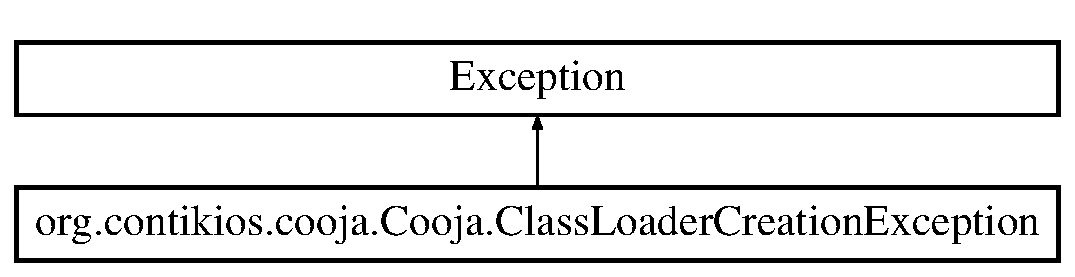
\includegraphics[height=2.000000cm]{classorg_1_1contikios_1_1cooja_1_1Cooja_1_1ClassLoaderCreationException}
\end{center}
\end{figure}
\subsection*{Public Member Functions}
\begin{DoxyCompactItemize}
\item 
\hypertarget{classorg_1_1contikios_1_1cooja_1_1Cooja_1_1ClassLoaderCreationException_a63b8dd151fb6c1f0bc3477fc28167d5a}{{\bfseries Class\-Loader\-Creation\-Exception} (String message)}\label{classorg_1_1contikios_1_1cooja_1_1Cooja_1_1ClassLoaderCreationException_a63b8dd151fb6c1f0bc3477fc28167d5a}

\end{DoxyCompactItemize}


The documentation for this class was generated from the following file\-:\begin{DoxyCompactItemize}
\item 
Cooja.\-java\end{DoxyCompactItemize}

\hypertarget{classorg_1_1contikios_1_1cooja_1_1ContikiError}{\section{org.\-contikios.\-cooja.\-Contiki\-Error Class Reference}
\label{classorg_1_1contikios_1_1cooja_1_1ContikiError}\index{org.\-contikios.\-cooja.\-Contiki\-Error@{org.\-contikios.\-cooja.\-Contiki\-Error}}
}
Inheritance diagram for org.\-contikios.\-cooja.\-Contiki\-Error\-:\begin{figure}[H]
\begin{center}
\leavevmode
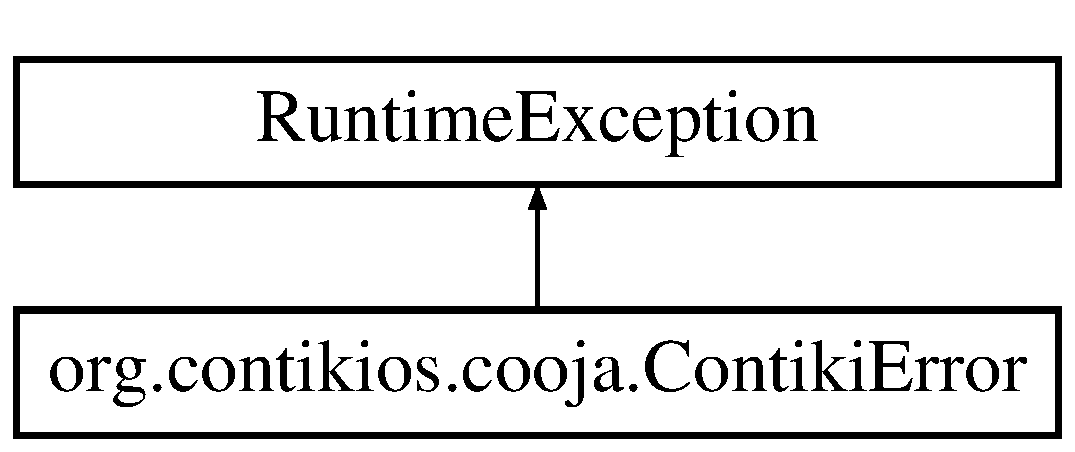
\includegraphics[height=2.000000cm]{classorg_1_1contikios_1_1cooja_1_1ContikiError}
\end{center}
\end{figure}
\subsection*{Public Member Functions}
\begin{DoxyCompactItemize}
\item 
\hypertarget{classorg_1_1contikios_1_1cooja_1_1ContikiError_a78e53f9f4b5afab00689b5a756e11c1a}{{\bfseries Contiki\-Error} (String message)}\label{classorg_1_1contikios_1_1cooja_1_1ContikiError_a78e53f9f4b5afab00689b5a756e11c1a}

\item 
\hypertarget{classorg_1_1contikios_1_1cooja_1_1ContikiError_af1b1ca40c9d6f6fdee7033dab73596d5}{String {\bfseries get\-Contiki\-Error} ()}\label{classorg_1_1contikios_1_1cooja_1_1ContikiError_af1b1ca40c9d6f6fdee7033dab73596d5}

\end{DoxyCompactItemize}


The documentation for this class was generated from the following file\-:\begin{DoxyCompactItemize}
\item 
Contiki\-Error.\-java\end{DoxyCompactItemize}

\hypertarget{classorg_1_1contikios_1_1cooja_1_1ConvertedRadioPacket}{\section{org.\-contikios.\-cooja.\-Converted\-Radio\-Packet Class Reference}
\label{classorg_1_1contikios_1_1cooja_1_1ConvertedRadioPacket}\index{org.\-contikios.\-cooja.\-Converted\-Radio\-Packet@{org.\-contikios.\-cooja.\-Converted\-Radio\-Packet}}
}
Inheritance diagram for org.\-contikios.\-cooja.\-Converted\-Radio\-Packet\-:\begin{figure}[H]
\begin{center}
\leavevmode
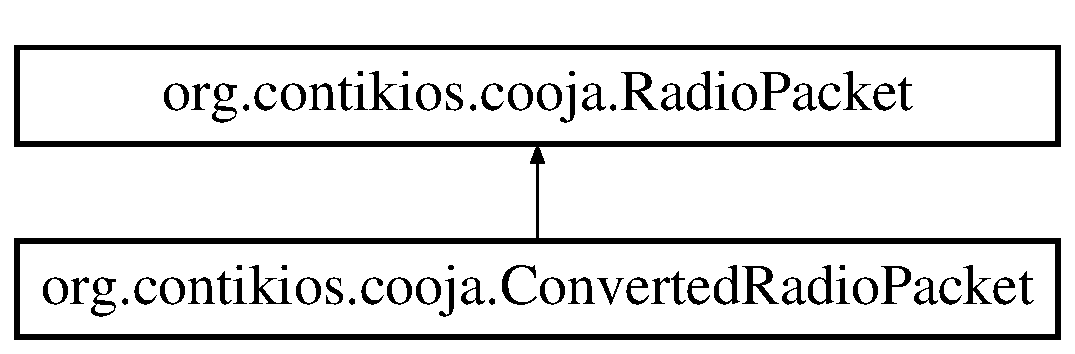
\includegraphics[height=2.000000cm]{classorg_1_1contikios_1_1cooja_1_1ConvertedRadioPacket}
\end{center}
\end{figure}
\subsection*{Public Member Functions}
\begin{DoxyCompactItemize}
\item 
\hypertarget{classorg_1_1contikios_1_1cooja_1_1ConvertedRadioPacket_a0a0b33a24aa62e24155260d2ebadbcf3}{{\bfseries Converted\-Radio\-Packet} (byte\mbox{[}$\,$\mbox{]} converted\-Data, byte\mbox{[}$\,$\mbox{]} original\-Data)}\label{classorg_1_1contikios_1_1cooja_1_1ConvertedRadioPacket_a0a0b33a24aa62e24155260d2ebadbcf3}

\item 
byte\mbox{[}$\,$\mbox{]} \hyperlink{classorg_1_1contikios_1_1cooja_1_1ConvertedRadioPacket_a2038c34dfd7e55daad454f8c34ddb33e}{get\-Packet\-Data} ()
\item 
\hypertarget{classorg_1_1contikios_1_1cooja_1_1ConvertedRadioPacket_a55d4161b57b17dec82908e7a7adc3f60}{byte\mbox{[}$\,$\mbox{]} {\bfseries get\-Original\-Packet\-Data} ()}\label{classorg_1_1contikios_1_1cooja_1_1ConvertedRadioPacket_a55d4161b57b17dec82908e7a7adc3f60}

\end{DoxyCompactItemize}


\subsection{Member Function Documentation}
\hypertarget{classorg_1_1contikios_1_1cooja_1_1ConvertedRadioPacket_a2038c34dfd7e55daad454f8c34ddb33e}{\index{org\-::contikios\-::cooja\-::\-Converted\-Radio\-Packet@{org\-::contikios\-::cooja\-::\-Converted\-Radio\-Packet}!get\-Packet\-Data@{get\-Packet\-Data}}
\index{get\-Packet\-Data@{get\-Packet\-Data}!org::contikios::cooja::ConvertedRadioPacket@{org\-::contikios\-::cooja\-::\-Converted\-Radio\-Packet}}
\subsubsection[{get\-Packet\-Data}]{\setlength{\rightskip}{0pt plus 5cm}byte \mbox{[}$\,$\mbox{]} org.\-contikios.\-cooja.\-Converted\-Radio\-Packet.\-get\-Packet\-Data (
\begin{DoxyParamCaption}
{}
\end{DoxyParamCaption}
)\hspace{0.3cm}{\ttfamily [inline]}}}\label{classorg_1_1contikios_1_1cooja_1_1ConvertedRadioPacket_a2038c34dfd7e55daad454f8c34ddb33e}
\begin{DoxyReturn}{Returns}
Packet data 
\end{DoxyReturn}


Implements \hyperlink{interfaceorg_1_1contikios_1_1cooja_1_1RadioPacket_aaff36d4c272ded32671f47ff68253415}{org.\-contikios.\-cooja.\-Radio\-Packet}.



The documentation for this class was generated from the following file\-:\begin{DoxyCompactItemize}
\item 
Converted\-Radio\-Packet.\-java\end{DoxyCompactItemize}

\hypertarget{classorg_1_1contikios_1_1cooja_1_1Cooja}{\section{org.\-contikios.\-cooja.\-Cooja Class Reference}
\label{classorg_1_1contikios_1_1cooja_1_1Cooja}\index{org.\-contikios.\-cooja.\-Cooja@{org.\-contikios.\-cooja.\-Cooja}}
}
Inheritance diagram for org.\-contikios.\-cooja.\-Cooja\-:\begin{figure}[H]
\begin{center}
\leavevmode
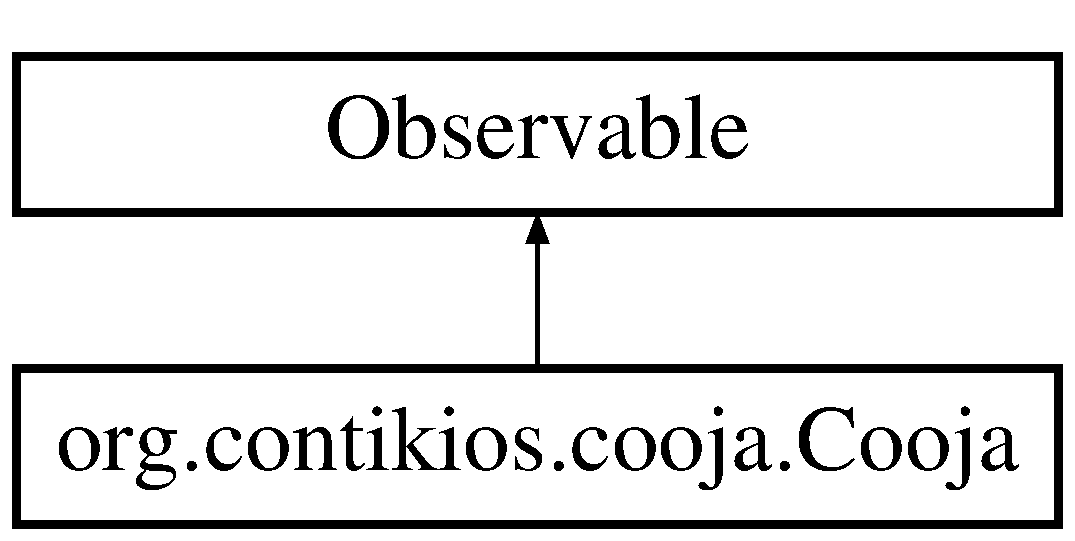
\includegraphics[height=2.000000cm]{classorg_1_1contikios_1_1cooja_1_1Cooja}
\end{center}
\end{figure}
\subsection*{Classes}
\begin{DoxyCompactItemize}
\item 
class \hyperlink{classorg_1_1contikios_1_1cooja_1_1Cooja_1_1ClassLoaderCreationException}{Class\-Loader\-Creation\-Exception}
\item 
class {\bfseries G\-U\-I\-Action}
\item 
class {\bfseries Mote\-Relation}
\item 
class \hyperlink{classorg_1_1contikios_1_1cooja_1_1Cooja_1_1ParseProjectsException}{Parse\-Projects\-Exception}
\item 
class \hyperlink{classorg_1_1contikios_1_1cooja_1_1Cooja_1_1PluginConstructionException}{Plugin\-Construction\-Exception}
\item 
class {\bfseries Runnable\-In\-E\-D\-T$<$ T $>$}
\item 
class \hyperlink{classorg_1_1contikios_1_1cooja_1_1Cooja_1_1SimulationCreationException}{Simulation\-Creation\-Exception}
\item 
class {\bfseries Start\-Plugin\-G\-U\-I\-Action}
\end{DoxyCompactItemize}
\subsection*{Public Member Functions}
\begin{DoxyCompactItemize}
\item 
\hyperlink{classorg_1_1contikios_1_1cooja_1_1Cooja_a2c7f9c93a2e946643755a6ab895299b5}{Cooja} (J\-Desktop\-Pane desktop)
\item 
void \hyperlink{classorg_1_1contikios_1_1cooja_1_1Cooja_afb7b606f3e30dfb4157190d8609f5c94}{add\-Mote\-Highlight\-Observer} (Observer new\-Observer)
\item 
void \hyperlink{classorg_1_1contikios_1_1cooja_1_1Cooja_aff35b66b1cfdf1868519864afefb69f1}{delete\-Mote\-Highlight\-Observer} (Observer observer)
\item 
void \hyperlink{classorg_1_1contikios_1_1cooja_1_1Cooja_ac6e4572107fbc8d51ff997ecfa2ba0d8}{set\-Visualized\-In\-Frame} (boolean visualized)
\item 
\hypertarget{classorg_1_1contikios_1_1cooja_1_1Cooja_a5119356c7801fd5f4dd95ca2cc6cfe88}{File {\bfseries get\-Last\-Opened\-File} ()}\label{classorg_1_1contikios_1_1cooja_1_1Cooja_a5119356c7801fd5f4dd95ca2cc6cfe88}

\item 
\hypertarget{classorg_1_1contikios_1_1cooja_1_1Cooja_a6627d55537ae3adc448d3880fc56afa7}{File\mbox{[}$\,$\mbox{]} {\bfseries get\-File\-History} ()}\label{classorg_1_1contikios_1_1cooja_1_1Cooja_a6627d55537ae3adc448d3880fc56afa7}

\item 
\hypertarget{classorg_1_1contikios_1_1cooja_1_1Cooja_a419fb67e62459ca3d629e6d20a2a9933}{void {\bfseries add\-To\-File\-History} (File file)}\label{classorg_1_1contikios_1_1cooja_1_1Cooja_a419fb67e62459ca3d629e6d20a2a9933}

\item 
J\-Desktop\-Pane \hyperlink{classorg_1_1contikios_1_1cooja_1_1Cooja_a02373668fc0ed84dc82dce4e031797c6}{get\-Desktop\-Pane} ()
\item 
void \hyperlink{classorg_1_1contikios_1_1cooja_1_1Cooja_acfbfd65613092e0b6fa743225cd577dc}{register\-Mote\-Type} (Class$<$?extends \hyperlink{interfaceorg_1_1contikios_1_1cooja_1_1MoteType}{Mote\-Type} $>$ mote\-Type\-Class)
\item 
void \hyperlink{classorg_1_1contikios_1_1cooja_1_1Cooja_ac350cadcee44d4660a3dc48e173207d3}{unregister\-Mote\-Types} ()
\item 
Vector$<$ Class$<$?extends \hyperlink{interfaceorg_1_1contikios_1_1cooja_1_1MoteType}{Mote\-Type} $>$ $>$ \hyperlink{classorg_1_1contikios_1_1cooja_1_1Cooja_a1e1841a06fec0ed49c524ac00710e897}{get\-Registered\-Mote\-Types} ()
\item 
boolean \hyperlink{classorg_1_1contikios_1_1cooja_1_1Cooja_aea29601f32712fcd5ddecd9711d55042}{register\-Positioner} (Class$<$?extends \hyperlink{classorg_1_1contikios_1_1cooja_1_1Positioner}{Positioner} $>$ positioner\-Class)
\item 
void \hyperlink{classorg_1_1contikios_1_1cooja_1_1Cooja_a73e4e8644e64b139128d40dce23896ca}{unregister\-Positioners} ()
\item 
Vector$<$ Class$<$?extends \\*
\hyperlink{classorg_1_1contikios_1_1cooja_1_1Positioner}{Positioner} $>$ $>$ \hyperlink{classorg_1_1contikios_1_1cooja_1_1Cooja_a502832bf7d93eae626274b641e4455f2}{get\-Registered\-Positioners} ()
\item 
boolean \hyperlink{classorg_1_1contikios_1_1cooja_1_1Cooja_a02d732370374ce1fc92fc731fb65d0b9}{register\-Radio\-Medium} (Class$<$?extends \hyperlink{classorg_1_1contikios_1_1cooja_1_1RadioMedium}{Radio\-Medium} $>$ radio\-Medium\-Class)
\item 
void \hyperlink{classorg_1_1contikios_1_1cooja_1_1Cooja_a9ae78c7e59efbf14f593d91d81430158}{unregister\-Radio\-Mediums} ()
\item 
Vector$<$ Class$<$?extends \\*
\hyperlink{classorg_1_1contikios_1_1cooja_1_1RadioMedium}{Radio\-Medium} $>$ $>$ \hyperlink{classorg_1_1contikios_1_1cooja_1_1Cooja_a4075ce3766cb2bbc40d2a3ddadd0189d}{get\-Registered\-Radio\-Mediums} ()
\item 
void \hyperlink{classorg_1_1contikios_1_1cooja_1_1Cooja_ae37f9adabef8d3f5186d2c71550dee7b}{reparse\-Project\-Config} ()  throws Parse\-Projects\-Exception 
\item 
\hyperlink{classorg_1_1contikios_1_1cooja_1_1ProjectConfig}{Project\-Config} \hyperlink{classorg_1_1contikios_1_1cooja_1_1Cooja_a57c3f5341a49924e2419b26ff374267f}{get\-Project\-Config} ()
\item 
\hyperlink{classorg_1_1contikios_1_1cooja_1_1COOJAProject}{C\-O\-O\-J\-A\-Project}\mbox{[}$\,$\mbox{]} \hyperlink{classorg_1_1contikios_1_1cooja_1_1Cooja_adda2fcf2fe42975c975859b062899434}{get\-Projects} ()
\item 
void \hyperlink{classorg_1_1contikios_1_1cooja_1_1Cooja_a16349cbb2017db876f1d5ef2bb6384c1}{show\-Plugin} (final \hyperlink{interfaceorg_1_1contikios_1_1cooja_1_1Plugin}{Plugin} plugin)
\item 
void \hyperlink{classorg_1_1contikios_1_1cooja_1_1Cooja_a366158a73ae30ab8b8a41b015c926022}{close\-Mote\-Plugins} (\hyperlink{interfaceorg_1_1contikios_1_1cooja_1_1Mote}{Mote} mote)
\item 
void \hyperlink{classorg_1_1contikios_1_1cooja_1_1Cooja_aa515697c688d47a06712703420558433}{remove\-Plugin} (final \hyperlink{interfaceorg_1_1contikios_1_1cooja_1_1Plugin}{Plugin} plugin, final boolean ask\-User)
\item 
\hypertarget{classorg_1_1contikios_1_1cooja_1_1Cooja_a1dfc83f2625490136b04d80bd7bec63c}{\hyperlink{interfaceorg_1_1contikios_1_1cooja_1_1Plugin}{Plugin} {\bfseries try\-Start\-Plugin} (final Class$<$?extends \hyperlink{interfaceorg_1_1contikios_1_1cooja_1_1Plugin}{Plugin} $>$ plugin\-Class, final \hyperlink{classorg_1_1contikios_1_1cooja_1_1Cooja}{Cooja} arg\-G\-U\-I, final \hyperlink{classorg_1_1contikios_1_1cooja_1_1Simulation}{Simulation} arg\-Simulation, final \hyperlink{interfaceorg_1_1contikios_1_1cooja_1_1Mote}{Mote} arg\-Mote)}\label{classorg_1_1contikios_1_1cooja_1_1Cooja_a1dfc83f2625490136b04d80bd7bec63c}

\item 
\hypertarget{classorg_1_1contikios_1_1cooja_1_1Cooja_a67e9f8928871005c0a13a0fddd337046}{\hyperlink{interfaceorg_1_1contikios_1_1cooja_1_1Plugin}{Plugin} {\bfseries start\-Plugin} (final Class$<$?extends \hyperlink{interfaceorg_1_1contikios_1_1cooja_1_1Plugin}{Plugin} $>$ plugin\-Class, final \hyperlink{classorg_1_1contikios_1_1cooja_1_1Cooja}{Cooja} arg\-G\-U\-I, final \hyperlink{classorg_1_1contikios_1_1cooja_1_1Simulation}{Simulation} arg\-Simulation, final \hyperlink{interfaceorg_1_1contikios_1_1cooja_1_1Mote}{Mote} arg\-Mote)  throws Plugin\-Construction\-Exception   }\label{classorg_1_1contikios_1_1cooja_1_1Cooja_a67e9f8928871005c0a13a0fddd337046}

\item 
void \hyperlink{classorg_1_1contikios_1_1cooja_1_1Cooja_ad46d017c3396ceb458b3fbe90056917a}{unregister\-Plugin} (Class$<$?extends \hyperlink{interfaceorg_1_1contikios_1_1cooja_1_1Plugin}{Plugin} $>$ plugin\-Class)
\item 
boolean \hyperlink{classorg_1_1contikios_1_1cooja_1_1Cooja_a1450321d34b37b5ea2f1e46806335482}{register\-Plugin} (final Class$<$?extends \hyperlink{interfaceorg_1_1contikios_1_1cooja_1_1Plugin}{Plugin} $>$ plugin\-Class)
\item 
void \hyperlink{classorg_1_1contikios_1_1cooja_1_1Cooja_acd8c2879d7778d06749d958cffb2fc06}{unregister\-Plugins} ()
\item 
\hyperlink{interfaceorg_1_1contikios_1_1cooja_1_1Plugin}{Plugin} \hyperlink{classorg_1_1contikios_1_1cooja_1_1Cooja_a3a490e5abdbecd18d31cf6272de00672}{get\-Plugin} (String classname)
\item 
\hyperlink{interfaceorg_1_1contikios_1_1cooja_1_1Plugin}{Plugin} \hyperlink{classorg_1_1contikios_1_1cooja_1_1Cooja_a53d5d25ef3b9a5c76b660f042dd461e4}{get\-Started\-Plugin} (String classname)
\item 
\hypertarget{classorg_1_1contikios_1_1cooja_1_1Cooja_a4ae72ec54e7ab614610aacb40f90ef16}{\hyperlink{interfaceorg_1_1contikios_1_1cooja_1_1Plugin}{Plugin}\mbox{[}$\,$\mbox{]} {\bfseries get\-Started\-Plugins} ()}\label{classorg_1_1contikios_1_1cooja_1_1Cooja_a4ae72ec54e7ab614610aacb40f90ef16}

\item 
\hypertarget{classorg_1_1contikios_1_1cooja_1_1Cooja_a57b652ba5793fd467ce214001a38a11c}{J\-Menu {\bfseries create\-Mote\-Plugins\-Submenu} (Class$<$?extends \hyperlink{interfaceorg_1_1contikios_1_1cooja_1_1Plugin}{Plugin} $>$ plugin\-Class)}\label{classorg_1_1contikios_1_1cooja_1_1Cooja_a57b652ba5793fd467ce214001a38a11c}

\item 
J\-Menu \hyperlink{classorg_1_1contikios_1_1cooja_1_1Cooja_a05c932e736bae89b68e5fc74fd6c6648}{create\-Mote\-Plugins\-Submenu} (\hyperlink{interfaceorg_1_1contikios_1_1cooja_1_1Mote}{Mote} mote)
\item 
\hyperlink{classorg_1_1contikios_1_1cooja_1_1Simulation}{Simulation} \hyperlink{classorg_1_1contikios_1_1cooja_1_1Cooja_a4b517e74a8b8405fd18d673079bf90bd}{get\-Simulation} ()
\item 
\hypertarget{classorg_1_1contikios_1_1cooja_1_1Cooja_a19e91b3fad20659743fcee6f8ccf5e2e}{void {\bfseries set\-Simulation} (\hyperlink{classorg_1_1contikios_1_1cooja_1_1Simulation}{Simulation} sim, boolean start\-Plugins)}\label{classorg_1_1contikios_1_1cooja_1_1Cooja_a19e91b3fad20659743fcee6f8ccf5e2e}

\item 
void \hyperlink{classorg_1_1contikios_1_1cooja_1_1Cooja_ad4852cfd6527e8e6abeb411f80032670}{do\-Create\-Mote\-Type} (Class$<$?extends \hyperlink{interfaceorg_1_1contikios_1_1cooja_1_1MoteType}{Mote\-Type} $>$ mote\-Type\-Class)
\item 
void \hyperlink{classorg_1_1contikios_1_1cooja_1_1Cooja_a1b9fc81beb44e643bed511a3bee541dd}{do\-Create\-Mote\-Type} (Class$<$?extends \hyperlink{interfaceorg_1_1contikios_1_1cooja_1_1MoteType}{Mote\-Type} $>$ mote\-Type\-Class, boolean add\-Motes)
\item 
boolean \hyperlink{classorg_1_1contikios_1_1cooja_1_1Cooja_a0b4e1f7e5a943baf9db5da0ccdca0493}{do\-Remove\-Simulation} (boolean ask\-For\-Confirmation)
\item 
void \hyperlink{classorg_1_1contikios_1_1cooja_1_1Cooja_a767dee33228ee6f1ef657b7afd832962}{do\-Load\-Config} (boolean ask\-For\-Confirmation, final boolean quick, File config\-File, Long manual\-Random\-Seed)
\item 
void \hyperlink{classorg_1_1contikios_1_1cooja_1_1Cooja_a61dd083fd9c8bfa0e06c4195fd6210e3}{reload\-Current\-Simulation} (final boolean auto\-Start, final long random\-Seed)
\item 
void \hyperlink{classorg_1_1contikios_1_1cooja_1_1Cooja_a93a8d5a584d9c69e10a07186bdc3f8de}{reload\-Current\-Simulation} (boolean auto\-Start)
\item 
File \hyperlink{classorg_1_1contikios_1_1cooja_1_1Cooja_aa870229cbaa13c431c6af992c27c67af}{do\-Save\-Config} (boolean ask\-For\-Confirmation)
\item 
void \hyperlink{classorg_1_1contikios_1_1cooja_1_1Cooja_a38fbde11ae2a5aad1731b2a3b9d908e5}{do\-Add\-Motes} (\hyperlink{interfaceorg_1_1contikios_1_1cooja_1_1MoteType}{Mote\-Type} mote\-Type)
\item 
void \hyperlink{classorg_1_1contikios_1_1cooja_1_1Cooja_ac4a6eb024ed2dc395408b4c68b38b8d8}{do\-Create\-Simulation} (boolean ask\-For\-Confirmation)
\item 
void \hyperlink{classorg_1_1contikios_1_1cooja_1_1Cooja_a67da2cf4e939c9243c6f75dee9a639d1}{do\-Quit} (boolean ask\-For\-Confirmation)
\item 
\hypertarget{classorg_1_1contikios_1_1cooja_1_1Cooja_a3de49ceeb26740628702f2536e38d5f0}{void {\bfseries do\-Quit} (boolean ask\-For\-Confirmation, int exit\-Code)}\label{classorg_1_1contikios_1_1cooja_1_1Cooja_a3de49ceeb26740628702f2536e38d5f0}

\item 
\hyperlink{classorg_1_1contikios_1_1cooja_1_1Simulation}{Simulation} \hyperlink{classorg_1_1contikios_1_1cooja_1_1Cooja_ac87c4fac26f6b5eb1d543857ca18d215}{load\-Simulation\-Config} (File file, boolean quick, Long manual\-Random\-Seed)  throws Unsatisfied\-Link\-Error, Simulation\-Creation\-Exception 
\item 
\hypertarget{classorg_1_1contikios_1_1cooja_1_1Cooja_a70cede41ba92811c2336a9952a7ec1c6}{\hyperlink{classorg_1_1contikios_1_1cooja_1_1Simulation}{Simulation} {\bfseries load\-Simulation\-Config} (Element root, boolean quick, Long manual\-Random\-Seed)  throws Simulation\-Creation\-Exception }\label{classorg_1_1contikios_1_1cooja_1_1Cooja_a70cede41ba92811c2336a9952a7ec1c6}

\item 
void \hyperlink{classorg_1_1contikios_1_1cooja_1_1Cooja_a480207a242c810a72524f25acc5333e4}{save\-Simulation\-Config} (File file)
\item 
\hypertarget{classorg_1_1contikios_1_1cooja_1_1Cooja_ac2479bd3e4a3d97f258a46bfb6c2d1f5}{Element {\bfseries extract\-Simulation\-Config} ()}\label{classorg_1_1contikios_1_1cooja_1_1Cooja_ac2479bd3e4a3d97f258a46bfb6c2d1f5}

\item 
Collection$<$ Element $>$ \hyperlink{classorg_1_1contikios_1_1cooja_1_1Cooja_a3700736fe7a56c54607848faade960b7}{get\-Plugins\-Config\-X\-M\-L} ()
\item 
\hypertarget{classorg_1_1contikios_1_1cooja_1_1Cooja_ab884045b7099fca29fa6f15a7a18c534}{boolean {\bfseries verify\-Projects} (Collection$<$ Element $>$ config\-X\-M\-L, boolean vis\-Available)}\label{classorg_1_1contikios_1_1cooja_1_1Cooja_ab884045b7099fca29fa6f15a7a18c534}

\item 
boolean \hyperlink{classorg_1_1contikios_1_1cooja_1_1Cooja_a533cf5b29d99909c3d5006410c50fcb3}{set\-Plugins\-Config\-X\-M\-L} (Collection$<$ Element $>$ config\-X\-M\-L, \hyperlink{classorg_1_1contikios_1_1cooja_1_1Simulation}{Simulation} simulation, boolean vis\-Available)
\item 
void \hyperlink{classorg_1_1contikios_1_1cooja_1_1Cooja_a33b977afa99c51bca0d2e804dfdd7ae1}{signal\-Mote\-Highlight} (\hyperlink{interfaceorg_1_1contikios_1_1cooja_1_1Mote}{Mote} m)
\item 
void \hyperlink{classorg_1_1contikios_1_1cooja_1_1Cooja_a39222d48cee0ec990dc9da2299c86273}{add\-Mote\-Relation} (\hyperlink{interfaceorg_1_1contikios_1_1cooja_1_1Mote}{Mote} source, \hyperlink{interfaceorg_1_1contikios_1_1cooja_1_1Mote}{Mote} dest)
\item 
void \hyperlink{classorg_1_1contikios_1_1cooja_1_1Cooja_afe30c2420481ee2c072d80346400c26e}{add\-Mote\-Relation} (\hyperlink{interfaceorg_1_1contikios_1_1cooja_1_1Mote}{Mote} source, \hyperlink{interfaceorg_1_1contikios_1_1cooja_1_1Mote}{Mote} dest, Color color)
\item 
void \hyperlink{classorg_1_1contikios_1_1cooja_1_1Cooja_adada775b6f36d1ee04b6ed97a8dc47ae}{remove\-Mote\-Relation} (\hyperlink{interfaceorg_1_1contikios_1_1cooja_1_1Mote}{Mote} source, \hyperlink{interfaceorg_1_1contikios_1_1cooja_1_1Mote}{Mote} dest)
\item 
Mote\-Relation\mbox{[}$\,$\mbox{]} \hyperlink{classorg_1_1contikios_1_1cooja_1_1Cooja_a7e42921b36012ba1f1056dbe5f1ffd04}{get\-Mote\-Relations} ()
\item 
void \hyperlink{classorg_1_1contikios_1_1cooja_1_1Cooja_a05178a0132e5acb0fbaf4f977094f46a}{add\-Mote\-Relations\-Observer} (Observer new\-Observer)
\item 
void \hyperlink{classorg_1_1contikios_1_1cooja_1_1Cooja_a57c8d4bee332f78c569f300b4ae937af}{delete\-Mote\-Relations\-Observer} (Observer observer)
\item 
File \hyperlink{classorg_1_1contikios_1_1cooja_1_1Cooja_aa6686d07c6bb986aed0920b49f954668}{create\-Portable\-Path} (File file)
\item 
\hypertarget{classorg_1_1contikios_1_1cooja_1_1Cooja_aacc90a0ccf8ecb1ff4f1318dd67f5d19}{File {\bfseries create\-Portable\-Path} (File file, boolean allow\-Config\-Relative\-Paths)}\label{classorg_1_1contikios_1_1cooja_1_1Cooja_aacc90a0ccf8ecb1ff4f1318dd67f5d19}

\item 
File \hyperlink{classorg_1_1contikios_1_1cooja_1_1Cooja_ae9e9345b095540569f17ec21edbd75f7}{restore\-Portable\-Path} (File file)
\item 
void \hyperlink{classorg_1_1contikios_1_1cooja_1_1Cooja_a835145d317bdb9fbbef855296df4d65e}{load\-Quick\-Help} (final Object obj)
\end{DoxyCompactItemize}
\subsection*{Static Public Member Functions}
\begin{DoxyCompactItemize}
\item 
static boolean \hyperlink{classorg_1_1contikios_1_1cooja_1_1Cooja_aa127774e211a01a333338c4434e9cd77}{is\-Visualized} ()
\item 
\hypertarget{classorg_1_1contikios_1_1cooja_1_1Cooja_a1a5a40f84add4ec6c49d090adfd8993e}{static Container {\bfseries get\-Top\-Parent\-Container} ()}\label{classorg_1_1contikios_1_1cooja_1_1Cooja_a1a5a40f84add4ec6c49d090adfd8993e}

\item 
\hypertarget{classorg_1_1contikios_1_1cooja_1_1Cooja_a88c28eb289131a1226a95970e11b7010}{static boolean {\bfseries is\-Visualized\-In\-Frame} ()}\label{classorg_1_1contikios_1_1cooja_1_1Cooja_a88c28eb289131a1226a95970e11b7010}

\item 
\hypertarget{classorg_1_1contikios_1_1cooja_1_1Cooja_ae92242683bcd34c7493c90900bac4e5a}{static U\-R\-L {\bfseries get\-Applet\-Code\-Base} ()}\label{classorg_1_1contikios_1_1cooja_1_1Cooja_ae92242683bcd34c7493c90900bac4e5a}

\item 
\hypertarget{classorg_1_1contikios_1_1cooja_1_1Cooja_a28b8e4ba3ccf4ae3b9ff0d92d09e23ea}{static boolean {\bfseries is\-Visualized\-In\-Applet} ()}\label{classorg_1_1contikios_1_1cooja_1_1Cooja_a28b8e4ba3ccf4ae3b9ff0d92d09e23ea}

\item 
\hypertarget{classorg_1_1contikios_1_1cooja_1_1Cooja_af32c56e136b759c60ac321b86fbee495}{static void {\bfseries set\-Look\-And\-Feel} ()}\label{classorg_1_1contikios_1_1cooja_1_1Cooja_af32c56e136b759c60ac321b86fbee495}

\item 
\hypertarget{classorg_1_1contikios_1_1cooja_1_1Cooja_a32e7dc5b4d7c2471746cf516bcbe7164}{static \hyperlink{classorg_1_1contikios_1_1cooja_1_1Simulation}{Simulation} {\bfseries quick\-Start\-Simulation\-Config} (File config, boolean vis, Long manual\-Random\-Seed)}\label{classorg_1_1contikios_1_1cooja_1_1Cooja_a32e7dc5b4d7c2471746cf516bcbe7164}

\item 
static int \hyperlink{classorg_1_1contikios_1_1cooja_1_1Cooja_add03d6c09080fa4591c9e4ed355eac71}{get\-External\-Tools\-Settings\-Count} ()
\item 
static String \hyperlink{classorg_1_1contikios_1_1cooja_1_1Cooja_ac2c460c7da1753ce5942e82f716f9ed5}{get\-External\-Tools\-Setting\-Name} (int index)
\item 
static String \hyperlink{classorg_1_1contikios_1_1cooja_1_1Cooja_a4a891672ef77e46ce486abb472bf1393}{get\-External\-Tools\-Setting} (String name)
\item 
static String \hyperlink{classorg_1_1contikios_1_1cooja_1_1Cooja_ad9b5e51fbc583c20fa32b1dcce124916}{get\-External\-Tools\-Setting} (String name, String default\-Value)
\item 
static String \hyperlink{classorg_1_1contikios_1_1cooja_1_1Cooja_a4e47d8ac0682f1e76dd27b7f0410570b}{get\-External\-Tools\-Default\-Setting} (String name, String default\-Value)
\item 
static void \hyperlink{classorg_1_1contikios_1_1cooja_1_1Cooja_a05369f1ac93204a267408c75a4db3e74}{set\-External\-Tools\-Setting} (String name, String new\-Val)
\item 
static void \hyperlink{classorg_1_1contikios_1_1cooja_1_1Cooja_a3c6349c155d43188f16016e48e71186d}{load\-External\-Tools\-Default\-Settings} ()
\item 
static void \hyperlink{classorg_1_1contikios_1_1cooja_1_1Cooja_a542b92835383b2a2da3a51e32fcae6e4}{load\-External\-Tools\-User\-Settings} ()
\item 
static void \hyperlink{classorg_1_1contikios_1_1cooja_1_1Cooja_ac3c796538b224b5e3277c98ecf013599}{save\-External\-Tools\-User\-Settings} ()
\item 
\hypertarget{classorg_1_1contikios_1_1cooja_1_1Cooja_a162ab2becc2d790de1d11d205c902149}{static File {\bfseries find\-Jar\-File} (File project\-Dir, String jarfile)}\label{classorg_1_1contikios_1_1cooja_1_1Cooja_a162ab2becc2d790de1d11d205c902149}

\item 
static String \hyperlink{classorg_1_1contikios_1_1cooja_1_1Cooja_af726e520e494a2f604d41193d2226a37}{get\-Description\-Of} (Object object)
\item 
static String \hyperlink{classorg_1_1contikios_1_1cooja_1_1Cooja_a7dbfbb75e29648bb5c0a9e2fa031fb2c}{get\-Description\-Of} (Class$<$?extends Object $>$ clazz)
\item 
static String \hyperlink{classorg_1_1contikios_1_1cooja_1_1Cooja_a87e6969953efa60ca8b6022b8f5fa303}{get\-Abstraction\-Level\-Description\-Of} (Class$<$?extends \hyperlink{interfaceorg_1_1contikios_1_1cooja_1_1MoteType}{Mote\-Type} $>$ clazz)
\item 
static void \hyperlink{classorg_1_1contikios_1_1cooja_1_1Cooja_a92add8a8932d7f4aab5940fe4ea2e387}{main} (String\mbox{[}$\,$\mbox{]} args)
\item 
static boolean \hyperlink{classorg_1_1contikios_1_1cooja_1_1Cooja_a1310bb137c102cc8daab0c313d4d4cee}{show\-Error\-Dialog} (final Component parent\-Component, final String title, final Throwable exception, final boolean retry\-Available)
\item 
\hypertarget{classorg_1_1contikios_1_1cooja_1_1Cooja_a1cfbf6bff9ea12170df5844c76b91a46}{static File {\bfseries restore\-Config\-Relative\-Path} (File config\-File, File portable)}\label{classorg_1_1contikios_1_1cooja_1_1Cooja_a1cfbf6bff9ea12170df5844c76b91a46}

\item 
\hypertarget{classorg_1_1contikios_1_1cooja_1_1Cooja_ae9960e57b2fc41870b90bf0ce141b770}{static void {\bfseries set\-Progress\-Message} (String msg)}\label{classorg_1_1contikios_1_1cooja_1_1Cooja_ae9960e57b2fc41870b90bf0ce141b770}

\item 
\hypertarget{classorg_1_1contikios_1_1cooja_1_1Cooja_acfb0128bba79cd55e99f76225e5d904b}{static void {\bfseries set\-Progress\-Message} (String msg, int type)}\label{classorg_1_1contikios_1_1cooja_1_1Cooja_acfb0128bba79cd55e99f76225e5d904b}

\end{DoxyCompactItemize}
\subsection*{Public Attributes}
\begin{DoxyCompactItemize}
\item 
\hypertarget{classorg_1_1contikios_1_1cooja_1_1Cooja_ae89632f463a9dab28324f33f407b4c28}{Class\-Loader {\bfseries project\-Dir\-Class\-Loader}}\label{classorg_1_1contikios_1_1cooja_1_1Cooja_ae89632f463a9dab28324f33f407b4c28}

\item 
\hypertarget{classorg_1_1contikios_1_1cooja_1_1Cooja_ae65cb892ceb2b39864c0359fba8267af}{File {\bfseries current\-Config\-File} = null}\label{classorg_1_1contikios_1_1cooja_1_1Cooja_ae65cb892ceb2b39864c0359fba8267af}

\end{DoxyCompactItemize}
\subsection*{Static Public Attributes}
\begin{DoxyCompactItemize}
\item 
static final String \hyperlink{classorg_1_1contikios_1_1cooja_1_1Cooja_ac8b53710bce8753270fcd8826ea539f9}{E\-X\-T\-E\-R\-N\-A\-L\-\_\-\-T\-O\-O\-L\-S\-\_\-\-S\-E\-T\-T\-I\-N\-G\-S\-\_\-\-F\-I\-L\-E\-N\-A\-M\-E} = \char`\"{}/external\-\_\-tools.\-config\char`\"{}
\item 
static final String \hyperlink{classorg_1_1contikios_1_1cooja_1_1Cooja_ac0b18524e403561cba19ab3276959e52}{E\-X\-T\-E\-R\-N\-A\-L\-\_\-\-T\-O\-O\-L\-S\-\_\-\-W\-I\-N32\-\_\-\-S\-E\-T\-T\-I\-N\-G\-S\-\_\-\-F\-I\-L\-E\-N\-A\-M\-E} = \char`\"{}/external\-\_\-tools\-\_\-win32.\-config\char`\"{}
\item 
static final String \hyperlink{classorg_1_1contikios_1_1cooja_1_1Cooja_a72a3d8502271a9fa5834c6ba5181d4a4}{E\-X\-T\-E\-R\-N\-A\-L\-\_\-\-T\-O\-O\-L\-S\-\_\-\-M\-A\-C\-O\-S\-X\-\_\-\-S\-E\-T\-T\-I\-N\-G\-S\-\_\-\-F\-I\-L\-E\-N\-A\-M\-E} = \char`\"{}/external\-\_\-tools\-\_\-macosx.\-config\char`\"{}
\item 
static final String \hyperlink{classorg_1_1contikios_1_1cooja_1_1Cooja_af201e3cdd7ce3ced1eb35725d30e1878}{E\-X\-T\-E\-R\-N\-A\-L\-\_\-\-T\-O\-O\-L\-S\-\_\-\-F\-R\-E\-E\-B\-S\-D\-\_\-\-S\-E\-T\-T\-I\-N\-G\-S\-\_\-\-F\-I\-L\-E\-N\-A\-M\-E} = \char`\"{}/external\-\_\-tools\-\_\-freebsd.\-config\char`\"{}
\item 
static final String \hyperlink{classorg_1_1contikios_1_1cooja_1_1Cooja_aed94a271d3a2f2fedf0f285aa065ed2c}{E\-X\-T\-E\-R\-N\-A\-L\-\_\-\-T\-O\-O\-L\-S\-\_\-\-L\-I\-N\-U\-X\-\_\-\-S\-E\-T\-T\-I\-N\-G\-S\-\_\-\-F\-I\-L\-E\-N\-A\-M\-E} = \char`\"{}/external\-\_\-tools\-\_\-linux.\-config\char`\"{}
\item 
static final String \hyperlink{classorg_1_1contikios_1_1cooja_1_1Cooja_a94c686a8440aea855f590d3cce89ad41}{E\-X\-T\-E\-R\-N\-A\-L\-\_\-\-T\-O\-O\-L\-S\-\_\-\-L\-I\-N\-U\-X\-\_\-64\-\_\-\-S\-E\-T\-T\-I\-N\-G\-S\-\_\-\-F\-I\-L\-E\-N\-A\-M\-E} = \char`\"{}/external\-\_\-tools\-\_\-linux\-\_\-64.\-config\char`\"{}
\item 
static final String \hyperlink{classorg_1_1contikios_1_1cooja_1_1Cooja_a3bdb7946630922d2dbbd00093113065d}{E\-X\-T\-E\-R\-N\-A\-L\-\_\-\-T\-O\-O\-L\-S\-\_\-\-U\-S\-E\-R\-\_\-\-S\-E\-T\-T\-I\-N\-G\-S\-\_\-\-F\-I\-L\-E\-N\-A\-M\-E} = \char`\"{}.cooja.\-user.\-properties\char`\"{}
\item 
\hypertarget{classorg_1_1contikios_1_1cooja_1_1Cooja_aaba23c0b94b4019d523762425fe83b76}{static File {\bfseries external\-Tools\-User\-Settings\-File}}\label{classorg_1_1contikios_1_1cooja_1_1Cooja_aaba23c0b94b4019d523762425fe83b76}

\item 
static final String \hyperlink{classorg_1_1contikios_1_1cooja_1_1Cooja_a427daf961354f0d5ba97e164895a4092}{L\-O\-G\-\_\-\-C\-O\-N\-F\-I\-G\-\_\-\-F\-I\-L\-E} = \char`\"{}log4j\-\_\-config.\-xml\char`\"{}
\item 
static String \hyperlink{classorg_1_1contikios_1_1cooja_1_1Cooja_aca1341e1789a5cb45b370458d20776a2}{P\-R\-O\-J\-E\-C\-T\-\_\-\-D\-E\-F\-A\-U\-L\-T\-\_\-\-C\-O\-N\-F\-I\-G\-\_\-\-F\-I\-L\-E\-N\-A\-M\-E} = null
\item 
static final String \hyperlink{classorg_1_1contikios_1_1cooja_1_1Cooja_a4cf31aa608d594c6f3318f3a001637c0}{P\-R\-O\-J\-E\-C\-T\-\_\-\-C\-O\-N\-F\-I\-G\-\_\-\-F\-I\-L\-E\-N\-A\-M\-E} = \char`\"{}cooja.\-config\char`\"{}
\item 
static final File\-Filter \hyperlink{classorg_1_1contikios_1_1cooja_1_1Cooja_a378fe78babb39ed68123203dc7ba01f4}{S\-A\-V\-E\-D\-\_\-\-S\-I\-M\-U\-L\-A\-T\-I\-O\-N\-S\-\_\-\-F\-I\-L\-E\-S}
\item 
\hypertarget{classorg_1_1contikios_1_1cooja_1_1Cooja_a2f018b27739bd5c70efceee3fb19dfea}{static Properties {\bfseries default\-External\-Tools\-Settings}}\label{classorg_1_1contikios_1_1cooja_1_1Cooja_a2f018b27739bd5c70efceee3fb19dfea}

\item 
\hypertarget{classorg_1_1contikios_1_1cooja_1_1Cooja_ae3bed99889fdc5d5c65c38f15c6f39fb}{static Properties {\bfseries current\-External\-Tools\-Settings}}\label{classorg_1_1contikios_1_1cooja_1_1Cooja_ae3bed99889fdc5d5c65c38f15c6f39fb}

\end{DoxyCompactItemize}
\subsection*{Protected Attributes}
\begin{DoxyCompactItemize}
\item 
\hypertarget{classorg_1_1contikios_1_1cooja_1_1Cooja_a951f03ffbc57eaf7c8ef13f3191905b9}{G\-U\-I\-Event\-Handler {\bfseries gui\-Event\-Handler} = new G\-U\-I\-Event\-Handler()}\label{classorg_1_1contikios_1_1cooja_1_1Cooja_a951f03ffbc57eaf7c8ef13f3191905b9}

\end{DoxyCompactItemize}


\subsection{Detailed Description}
Main file of C\-O\-O\-J\-A Simulator. Typically contains a visualizer for the simulator, but can also be started without visualizer.

This class loads external Java classes (in extension directories), and handles the C\-O\-O\-J\-A plugins as well as the configuration system. If provides a number of help methods for the rest of the C\-O\-O\-J\-A system, and is the starting point for loading and saving simulation configs.

\begin{DoxyAuthor}{Author}
Fredrik Osterlind 
\end{DoxyAuthor}


\subsection{Constructor \& Destructor Documentation}
\hypertarget{classorg_1_1contikios_1_1cooja_1_1Cooja_a2c7f9c93a2e946643755a6ab895299b5}{\index{org\-::contikios\-::cooja\-::\-Cooja@{org\-::contikios\-::cooja\-::\-Cooja}!Cooja@{Cooja}}
\index{Cooja@{Cooja}!org::contikios::cooja::Cooja@{org\-::contikios\-::cooja\-::\-Cooja}}
\subsubsection[{Cooja}]{\setlength{\rightskip}{0pt plus 5cm}org.\-contikios.\-cooja.\-Cooja.\-Cooja (
\begin{DoxyParamCaption}
\item[{J\-Desktop\-Pane}]{desktop}
\end{DoxyParamCaption}
)\hspace{0.3cm}{\ttfamily [inline]}}}\label{classorg_1_1contikios_1_1cooja_1_1Cooja_a2c7f9c93a2e946643755a6ab895299b5}
Creates a new C\-O\-O\-J\-A Simulator G\-U\-I.


\begin{DoxyParams}{Parameters}
{\em desktop} & Desktop pane \\
\hline
\end{DoxyParams}


\subsection{Member Function Documentation}
\hypertarget{classorg_1_1contikios_1_1cooja_1_1Cooja_afb7b606f3e30dfb4157190d8609f5c94}{\index{org\-::contikios\-::cooja\-::\-Cooja@{org\-::contikios\-::cooja\-::\-Cooja}!add\-Mote\-Highlight\-Observer@{add\-Mote\-Highlight\-Observer}}
\index{add\-Mote\-Highlight\-Observer@{add\-Mote\-Highlight\-Observer}!org::contikios::cooja::Cooja@{org\-::contikios\-::cooja\-::\-Cooja}}
\subsubsection[{add\-Mote\-Highlight\-Observer}]{\setlength{\rightskip}{0pt plus 5cm}void org.\-contikios.\-cooja.\-Cooja.\-add\-Mote\-Highlight\-Observer (
\begin{DoxyParamCaption}
\item[{Observer}]{new\-Observer}
\end{DoxyParamCaption}
)\hspace{0.3cm}{\ttfamily [inline]}}}\label{classorg_1_1contikios_1_1cooja_1_1Cooja_afb7b606f3e30dfb4157190d8609f5c94}
Add mote highlight observer.

\begin{DoxySeeAlso}{See Also}
\hyperlink{classorg_1_1contikios_1_1cooja_1_1Cooja_aff35b66b1cfdf1868519864afefb69f1}{delete\-Mote\-Highlight\-Observer(\-Observer)} 
\end{DoxySeeAlso}

\begin{DoxyParams}{Parameters}
{\em new\-Observer} & New observer \\
\hline
\end{DoxyParams}
\hypertarget{classorg_1_1contikios_1_1cooja_1_1Cooja_a39222d48cee0ec990dc9da2299c86273}{\index{org\-::contikios\-::cooja\-::\-Cooja@{org\-::contikios\-::cooja\-::\-Cooja}!add\-Mote\-Relation@{add\-Mote\-Relation}}
\index{add\-Mote\-Relation@{add\-Mote\-Relation}!org::contikios::cooja::Cooja@{org\-::contikios\-::cooja\-::\-Cooja}}
\subsubsection[{add\-Mote\-Relation}]{\setlength{\rightskip}{0pt plus 5cm}void org.\-contikios.\-cooja.\-Cooja.\-add\-Mote\-Relation (
\begin{DoxyParamCaption}
\item[{{\bf Mote}}]{source, }
\item[{{\bf Mote}}]{dest}
\end{DoxyParamCaption}
)\hspace{0.3cm}{\ttfamily [inline]}}}\label{classorg_1_1contikios_1_1cooja_1_1Cooja_a39222d48cee0ec990dc9da2299c86273}
Adds directed relation between given motes.


\begin{DoxyParams}{Parameters}
{\em source} & Source mote \\
\hline
{\em dest} & Destination mote \\
\hline
\end{DoxyParams}
\hypertarget{classorg_1_1contikios_1_1cooja_1_1Cooja_afe30c2420481ee2c072d80346400c26e}{\index{org\-::contikios\-::cooja\-::\-Cooja@{org\-::contikios\-::cooja\-::\-Cooja}!add\-Mote\-Relation@{add\-Mote\-Relation}}
\index{add\-Mote\-Relation@{add\-Mote\-Relation}!org::contikios::cooja::Cooja@{org\-::contikios\-::cooja\-::\-Cooja}}
\subsubsection[{add\-Mote\-Relation}]{\setlength{\rightskip}{0pt plus 5cm}void org.\-contikios.\-cooja.\-Cooja.\-add\-Mote\-Relation (
\begin{DoxyParamCaption}
\item[{{\bf Mote}}]{source, }
\item[{{\bf Mote}}]{dest, }
\item[{Color}]{color}
\end{DoxyParamCaption}
)\hspace{0.3cm}{\ttfamily [inline]}}}\label{classorg_1_1contikios_1_1cooja_1_1Cooja_afe30c2420481ee2c072d80346400c26e}
Adds directed relation between given motes.


\begin{DoxyParams}{Parameters}
{\em source} & Source mote \\
\hline
{\em dest} & Destination mote \\
\hline
{\em color} & The color to use when visualizing the mote relation \\
\hline
\end{DoxyParams}
\hypertarget{classorg_1_1contikios_1_1cooja_1_1Cooja_a05178a0132e5acb0fbaf4f977094f46a}{\index{org\-::contikios\-::cooja\-::\-Cooja@{org\-::contikios\-::cooja\-::\-Cooja}!add\-Mote\-Relations\-Observer@{add\-Mote\-Relations\-Observer}}
\index{add\-Mote\-Relations\-Observer@{add\-Mote\-Relations\-Observer}!org::contikios::cooja::Cooja@{org\-::contikios\-::cooja\-::\-Cooja}}
\subsubsection[{add\-Mote\-Relations\-Observer}]{\setlength{\rightskip}{0pt plus 5cm}void org.\-contikios.\-cooja.\-Cooja.\-add\-Mote\-Relations\-Observer (
\begin{DoxyParamCaption}
\item[{Observer}]{new\-Observer}
\end{DoxyParamCaption}
)\hspace{0.3cm}{\ttfamily [inline]}}}\label{classorg_1_1contikios_1_1cooja_1_1Cooja_a05178a0132e5acb0fbaf4f977094f46a}
Adds mote relation observer. Typically used by visualizer plugins.


\begin{DoxyParams}{Parameters}
{\em new\-Observer} & Observer \\
\hline
\end{DoxyParams}
\hypertarget{classorg_1_1contikios_1_1cooja_1_1Cooja_a366158a73ae30ab8b8a41b015c926022}{\index{org\-::contikios\-::cooja\-::\-Cooja@{org\-::contikios\-::cooja\-::\-Cooja}!close\-Mote\-Plugins@{close\-Mote\-Plugins}}
\index{close\-Mote\-Plugins@{close\-Mote\-Plugins}!org::contikios::cooja::Cooja@{org\-::contikios\-::cooja\-::\-Cooja}}
\subsubsection[{close\-Mote\-Plugins}]{\setlength{\rightskip}{0pt plus 5cm}void org.\-contikios.\-cooja.\-Cooja.\-close\-Mote\-Plugins (
\begin{DoxyParamCaption}
\item[{{\bf Mote}}]{mote}
\end{DoxyParamCaption}
)\hspace{0.3cm}{\ttfamily [inline]}}}\label{classorg_1_1contikios_1_1cooja_1_1Cooja_a366158a73ae30ab8b8a41b015c926022}
Close all mote plugins for given mote.


\begin{DoxyParams}{Parameters}
{\em mote} & \hyperlink{interfaceorg_1_1contikios_1_1cooja_1_1Mote}{Mote} \\
\hline
\end{DoxyParams}
\hypertarget{classorg_1_1contikios_1_1cooja_1_1Cooja_a05c932e736bae89b68e5fc74fd6c6648}{\index{org\-::contikios\-::cooja\-::\-Cooja@{org\-::contikios\-::cooja\-::\-Cooja}!create\-Mote\-Plugins\-Submenu@{create\-Mote\-Plugins\-Submenu}}
\index{create\-Mote\-Plugins\-Submenu@{create\-Mote\-Plugins\-Submenu}!org::contikios::cooja::Cooja@{org\-::contikios\-::cooja\-::\-Cooja}}
\subsubsection[{create\-Mote\-Plugins\-Submenu}]{\setlength{\rightskip}{0pt plus 5cm}J\-Menu org.\-contikios.\-cooja.\-Cooja.\-create\-Mote\-Plugins\-Submenu (
\begin{DoxyParamCaption}
\item[{{\bf Mote}}]{mote}
\end{DoxyParamCaption}
)\hspace{0.3cm}{\ttfamily [inline]}}}\label{classorg_1_1contikios_1_1cooja_1_1Cooja_a05c932e736bae89b68e5fc74fd6c6648}
Return a mote plugins submenu for given mote.


\begin{DoxyParams}{Parameters}
{\em mote} & \hyperlink{interfaceorg_1_1contikios_1_1cooja_1_1Mote}{Mote} \\
\hline
\end{DoxyParams}
\begin{DoxyReturn}{Returns}
\hyperlink{interfaceorg_1_1contikios_1_1cooja_1_1Mote}{Mote} plugins menu 
\end{DoxyReturn}
\hypertarget{classorg_1_1contikios_1_1cooja_1_1Cooja_aa6686d07c6bb986aed0920b49f954668}{\index{org\-::contikios\-::cooja\-::\-Cooja@{org\-::contikios\-::cooja\-::\-Cooja}!create\-Portable\-Path@{create\-Portable\-Path}}
\index{create\-Portable\-Path@{create\-Portable\-Path}!org::contikios::cooja::Cooja@{org\-::contikios\-::cooja\-::\-Cooja}}
\subsubsection[{create\-Portable\-Path}]{\setlength{\rightskip}{0pt plus 5cm}File org.\-contikios.\-cooja.\-Cooja.\-create\-Portable\-Path (
\begin{DoxyParamCaption}
\item[{File}]{file}
\end{DoxyParamCaption}
)\hspace{0.3cm}{\ttfamily [inline]}}}\label{classorg_1_1contikios_1_1cooja_1_1Cooja_aa6686d07c6bb986aed0920b49f954668}
Tries to convert given file to be \char`\"{}portable\char`\"{}. The portable path is either relative to Contiki, or to the configuration (.csc) file.

If this method fails, it returns the original file.


\begin{DoxyParams}{Parameters}
{\em file} & Original file \\
\hline
\end{DoxyParams}
\begin{DoxyReturn}{Returns}
Portable file, or original file is conversion failed 
\end{DoxyReturn}
\hypertarget{classorg_1_1contikios_1_1cooja_1_1Cooja_aff35b66b1cfdf1868519864afefb69f1}{\index{org\-::contikios\-::cooja\-::\-Cooja@{org\-::contikios\-::cooja\-::\-Cooja}!delete\-Mote\-Highlight\-Observer@{delete\-Mote\-Highlight\-Observer}}
\index{delete\-Mote\-Highlight\-Observer@{delete\-Mote\-Highlight\-Observer}!org::contikios::cooja::Cooja@{org\-::contikios\-::cooja\-::\-Cooja}}
\subsubsection[{delete\-Mote\-Highlight\-Observer}]{\setlength{\rightskip}{0pt plus 5cm}void org.\-contikios.\-cooja.\-Cooja.\-delete\-Mote\-Highlight\-Observer (
\begin{DoxyParamCaption}
\item[{Observer}]{observer}
\end{DoxyParamCaption}
)\hspace{0.3cm}{\ttfamily [inline]}}}\label{classorg_1_1contikios_1_1cooja_1_1Cooja_aff35b66b1cfdf1868519864afefb69f1}
Delete mote highlight observer.

\begin{DoxySeeAlso}{See Also}
\hyperlink{classorg_1_1contikios_1_1cooja_1_1Cooja_afb7b606f3e30dfb4157190d8609f5c94}{add\-Mote\-Highlight\-Observer(\-Observer)} 
\end{DoxySeeAlso}

\begin{DoxyParams}{Parameters}
{\em observer} & Observer to delete \\
\hline
\end{DoxyParams}
\hypertarget{classorg_1_1contikios_1_1cooja_1_1Cooja_a57c8d4bee332f78c569f300b4ae937af}{\index{org\-::contikios\-::cooja\-::\-Cooja@{org\-::contikios\-::cooja\-::\-Cooja}!delete\-Mote\-Relations\-Observer@{delete\-Mote\-Relations\-Observer}}
\index{delete\-Mote\-Relations\-Observer@{delete\-Mote\-Relations\-Observer}!org::contikios::cooja::Cooja@{org\-::contikios\-::cooja\-::\-Cooja}}
\subsubsection[{delete\-Mote\-Relations\-Observer}]{\setlength{\rightskip}{0pt plus 5cm}void org.\-contikios.\-cooja.\-Cooja.\-delete\-Mote\-Relations\-Observer (
\begin{DoxyParamCaption}
\item[{Observer}]{observer}
\end{DoxyParamCaption}
)\hspace{0.3cm}{\ttfamily [inline]}}}\label{classorg_1_1contikios_1_1cooja_1_1Cooja_a57c8d4bee332f78c569f300b4ae937af}
Removes mote relation observer. Typically used by visualizer plugins.


\begin{DoxyParams}{Parameters}
{\em observer} & Observer \\
\hline
\end{DoxyParams}
\hypertarget{classorg_1_1contikios_1_1cooja_1_1Cooja_a38fbde11ae2a5aad1731b2a3b9d908e5}{\index{org\-::contikios\-::cooja\-::\-Cooja@{org\-::contikios\-::cooja\-::\-Cooja}!do\-Add\-Motes@{do\-Add\-Motes}}
\index{do\-Add\-Motes@{do\-Add\-Motes}!org::contikios::cooja::Cooja@{org\-::contikios\-::cooja\-::\-Cooja}}
\subsubsection[{do\-Add\-Motes}]{\setlength{\rightskip}{0pt plus 5cm}void org.\-contikios.\-cooja.\-Cooja.\-do\-Add\-Motes (
\begin{DoxyParamCaption}
\item[{{\bf Mote\-Type}}]{mote\-Type}
\end{DoxyParamCaption}
)\hspace{0.3cm}{\ttfamily [inline]}}}\label{classorg_1_1contikios_1_1cooja_1_1Cooja_a38fbde11ae2a5aad1731b2a3b9d908e5}
Add new mote to current simulation \hypertarget{classorg_1_1contikios_1_1cooja_1_1Cooja_ad4852cfd6527e8e6abeb411f80032670}{\index{org\-::contikios\-::cooja\-::\-Cooja@{org\-::contikios\-::cooja\-::\-Cooja}!do\-Create\-Mote\-Type@{do\-Create\-Mote\-Type}}
\index{do\-Create\-Mote\-Type@{do\-Create\-Mote\-Type}!org::contikios::cooja::Cooja@{org\-::contikios\-::cooja\-::\-Cooja}}
\subsubsection[{do\-Create\-Mote\-Type}]{\setlength{\rightskip}{0pt plus 5cm}void org.\-contikios.\-cooja.\-Cooja.\-do\-Create\-Mote\-Type (
\begin{DoxyParamCaption}
\item[{Class$<$?extends {\bf Mote\-Type} $>$}]{mote\-Type\-Class}
\end{DoxyParamCaption}
)\hspace{0.3cm}{\ttfamily [inline]}}}\label{classorg_1_1contikios_1_1cooja_1_1Cooja_ad4852cfd6527e8e6abeb411f80032670}
Creates a new mote type of the given mote type class. This may include displaying a dialog for user configurations.

If mote type is created successfully, the add motes dialog will appear.


\begin{DoxyParams}{Parameters}
{\em mote\-Type\-Class} & \hyperlink{interfaceorg_1_1contikios_1_1cooja_1_1Mote}{Mote} type class \\
\hline
\end{DoxyParams}
\hypertarget{classorg_1_1contikios_1_1cooja_1_1Cooja_a1b9fc81beb44e643bed511a3bee541dd}{\index{org\-::contikios\-::cooja\-::\-Cooja@{org\-::contikios\-::cooja\-::\-Cooja}!do\-Create\-Mote\-Type@{do\-Create\-Mote\-Type}}
\index{do\-Create\-Mote\-Type@{do\-Create\-Mote\-Type}!org::contikios::cooja::Cooja@{org\-::contikios\-::cooja\-::\-Cooja}}
\subsubsection[{do\-Create\-Mote\-Type}]{\setlength{\rightskip}{0pt plus 5cm}void org.\-contikios.\-cooja.\-Cooja.\-do\-Create\-Mote\-Type (
\begin{DoxyParamCaption}
\item[{Class$<$?extends {\bf Mote\-Type} $>$}]{mote\-Type\-Class, }
\item[{boolean}]{add\-Motes}
\end{DoxyParamCaption}
)\hspace{0.3cm}{\ttfamily [inline]}}}\label{classorg_1_1contikios_1_1cooja_1_1Cooja_a1b9fc81beb44e643bed511a3bee541dd}
Creates a new mote type of the given mote type class. This may include displaying a dialog for user configurations.


\begin{DoxyParams}{Parameters}
{\em mote\-Type\-Class} & \hyperlink{interfaceorg_1_1contikios_1_1cooja_1_1Mote}{Mote} type class \\
\hline
{\em add\-Motes} & Show add motes dialog after successfully adding mote type \\
\hline
\end{DoxyParams}
\hypertarget{classorg_1_1contikios_1_1cooja_1_1Cooja_ac4a6eb024ed2dc395408b4c68b38b8d8}{\index{org\-::contikios\-::cooja\-::\-Cooja@{org\-::contikios\-::cooja\-::\-Cooja}!do\-Create\-Simulation@{do\-Create\-Simulation}}
\index{do\-Create\-Simulation@{do\-Create\-Simulation}!org::contikios::cooja::Cooja@{org\-::contikios\-::cooja\-::\-Cooja}}
\subsubsection[{do\-Create\-Simulation}]{\setlength{\rightskip}{0pt plus 5cm}void org.\-contikios.\-cooja.\-Cooja.\-do\-Create\-Simulation (
\begin{DoxyParamCaption}
\item[{boolean}]{ask\-For\-Confirmation}
\end{DoxyParamCaption}
)\hspace{0.3cm}{\ttfamily [inline]}}}\label{classorg_1_1contikios_1_1cooja_1_1Cooja_ac4a6eb024ed2dc395408b4c68b38b8d8}
Create a new simulation


\begin{DoxyParams}{Parameters}
{\em ask\-For\-Confirmation} & Should we ask for confirmation if a simulation is already active? \\
\hline
\end{DoxyParams}
\hypertarget{classorg_1_1contikios_1_1cooja_1_1Cooja_a767dee33228ee6f1ef657b7afd832962}{\index{org\-::contikios\-::cooja\-::\-Cooja@{org\-::contikios\-::cooja\-::\-Cooja}!do\-Load\-Config@{do\-Load\-Config}}
\index{do\-Load\-Config@{do\-Load\-Config}!org::contikios::cooja::Cooja@{org\-::contikios\-::cooja\-::\-Cooja}}
\subsubsection[{do\-Load\-Config}]{\setlength{\rightskip}{0pt plus 5cm}void org.\-contikios.\-cooja.\-Cooja.\-do\-Load\-Config (
\begin{DoxyParamCaption}
\item[{boolean}]{ask\-For\-Confirmation, }
\item[{final boolean}]{quick, }
\item[{File}]{config\-File, }
\item[{Long}]{manual\-Random\-Seed}
\end{DoxyParamCaption}
)\hspace{0.3cm}{\ttfamily [inline]}}}\label{classorg_1_1contikios_1_1cooja_1_1Cooja_a767dee33228ee6f1ef657b7afd832962}
Load a simulation configuration file from disk


\begin{DoxyParams}{Parameters}
{\em ask\-For\-Confirmation} & Ask for confirmation before removing any current simulation \\
\hline
{\em quick} & Quick-\/load simulation \\
\hline
{\em config\-File} & Configuration file to load, if null a dialog will appear \\
\hline
\end{DoxyParams}
\hypertarget{classorg_1_1contikios_1_1cooja_1_1Cooja_a67da2cf4e939c9243c6f75dee9a639d1}{\index{org\-::contikios\-::cooja\-::\-Cooja@{org\-::contikios\-::cooja\-::\-Cooja}!do\-Quit@{do\-Quit}}
\index{do\-Quit@{do\-Quit}!org::contikios::cooja::Cooja@{org\-::contikios\-::cooja\-::\-Cooja}}
\subsubsection[{do\-Quit}]{\setlength{\rightskip}{0pt plus 5cm}void org.\-contikios.\-cooja.\-Cooja.\-do\-Quit (
\begin{DoxyParamCaption}
\item[{boolean}]{ask\-For\-Confirmation}
\end{DoxyParamCaption}
)\hspace{0.3cm}{\ttfamily [inline]}}}\label{classorg_1_1contikios_1_1cooja_1_1Cooja_a67da2cf4e939c9243c6f75dee9a639d1}
Quit program


\begin{DoxyParams}{Parameters}
{\em ask\-For\-Confirmation} & Should we ask for confirmation before quitting? \\
\hline
\end{DoxyParams}
\hypertarget{classorg_1_1contikios_1_1cooja_1_1Cooja_a0b4e1f7e5a943baf9db5da0ccdca0493}{\index{org\-::contikios\-::cooja\-::\-Cooja@{org\-::contikios\-::cooja\-::\-Cooja}!do\-Remove\-Simulation@{do\-Remove\-Simulation}}
\index{do\-Remove\-Simulation@{do\-Remove\-Simulation}!org::contikios::cooja::Cooja@{org\-::contikios\-::cooja\-::\-Cooja}}
\subsubsection[{do\-Remove\-Simulation}]{\setlength{\rightskip}{0pt plus 5cm}boolean org.\-contikios.\-cooja.\-Cooja.\-do\-Remove\-Simulation (
\begin{DoxyParamCaption}
\item[{boolean}]{ask\-For\-Confirmation}
\end{DoxyParamCaption}
)\hspace{0.3cm}{\ttfamily [inline]}}}\label{classorg_1_1contikios_1_1cooja_1_1Cooja_a0b4e1f7e5a943baf9db5da0ccdca0493}
Remove current simulation


\begin{DoxyParams}{Parameters}
{\em ask\-For\-Confirmation} & Should we ask for confirmation if a simulation is already active? \\
\hline
\end{DoxyParams}
\begin{DoxyReturn}{Returns}
True if no simulation exists when method returns 
\end{DoxyReturn}
\hypertarget{classorg_1_1contikios_1_1cooja_1_1Cooja_aa870229cbaa13c431c6af992c27c67af}{\index{org\-::contikios\-::cooja\-::\-Cooja@{org\-::contikios\-::cooja\-::\-Cooja}!do\-Save\-Config@{do\-Save\-Config}}
\index{do\-Save\-Config@{do\-Save\-Config}!org::contikios::cooja::Cooja@{org\-::contikios\-::cooja\-::\-Cooja}}
\subsubsection[{do\-Save\-Config}]{\setlength{\rightskip}{0pt plus 5cm}File org.\-contikios.\-cooja.\-Cooja.\-do\-Save\-Config (
\begin{DoxyParamCaption}
\item[{boolean}]{ask\-For\-Confirmation}
\end{DoxyParamCaption}
)\hspace{0.3cm}{\ttfamily [inline]}}}\label{classorg_1_1contikios_1_1cooja_1_1Cooja_aa870229cbaa13c431c6af992c27c67af}
Save current simulation configuration to disk


\begin{DoxyParams}{Parameters}
{\em ask\-For\-Confirmation} & Ask for confirmation before overwriting file \\
\hline
\end{DoxyParams}
\hypertarget{classorg_1_1contikios_1_1cooja_1_1Cooja_a87e6969953efa60ca8b6022b8f5fa303}{\index{org\-::contikios\-::cooja\-::\-Cooja@{org\-::contikios\-::cooja\-::\-Cooja}!get\-Abstraction\-Level\-Description\-Of@{get\-Abstraction\-Level\-Description\-Of}}
\index{get\-Abstraction\-Level\-Description\-Of@{get\-Abstraction\-Level\-Description\-Of}!org::contikios::cooja::Cooja@{org\-::contikios\-::cooja\-::\-Cooja}}
\subsubsection[{get\-Abstraction\-Level\-Description\-Of}]{\setlength{\rightskip}{0pt plus 5cm}static String org.\-contikios.\-cooja.\-Cooja.\-get\-Abstraction\-Level\-Description\-Of (
\begin{DoxyParamCaption}
\item[{Class$<$?extends {\bf Mote\-Type} $>$}]{clazz}
\end{DoxyParamCaption}
)\hspace{0.3cm}{\ttfamily [inline]}, {\ttfamily [static]}}}\label{classorg_1_1contikios_1_1cooja_1_1Cooja_a87e6969953efa60ca8b6022b8f5fa303}
Help method that returns the abstraction level description for given mote type class.


\begin{DoxyParams}{Parameters}
{\em clazz} & Class \\
\hline
\end{DoxyParams}
\begin{DoxyReturn}{Returns}
Description 
\end{DoxyReturn}
\hypertarget{classorg_1_1contikios_1_1cooja_1_1Cooja_af726e520e494a2f604d41193d2226a37}{\index{org\-::contikios\-::cooja\-::\-Cooja@{org\-::contikios\-::cooja\-::\-Cooja}!get\-Description\-Of@{get\-Description\-Of}}
\index{get\-Description\-Of@{get\-Description\-Of}!org::contikios::cooja::Cooja@{org\-::contikios\-::cooja\-::\-Cooja}}
\subsubsection[{get\-Description\-Of}]{\setlength{\rightskip}{0pt plus 5cm}static String org.\-contikios.\-cooja.\-Cooja.\-get\-Description\-Of (
\begin{DoxyParamCaption}
\item[{Object}]{object}
\end{DoxyParamCaption}
)\hspace{0.3cm}{\ttfamily [inline]}, {\ttfamily [static]}}}\label{classorg_1_1contikios_1_1cooja_1_1Cooja_af726e520e494a2f604d41193d2226a37}
Help method that returns the description for given object. This method reads from the object's class annotations if existing. Otherwise it returns the simple class name of object's class.


\begin{DoxyParams}{Parameters}
{\em object} & Object \\
\hline
\end{DoxyParams}
\begin{DoxyReturn}{Returns}
Description 
\end{DoxyReturn}
\hypertarget{classorg_1_1contikios_1_1cooja_1_1Cooja_a7dbfbb75e29648bb5c0a9e2fa031fb2c}{\index{org\-::contikios\-::cooja\-::\-Cooja@{org\-::contikios\-::cooja\-::\-Cooja}!get\-Description\-Of@{get\-Description\-Of}}
\index{get\-Description\-Of@{get\-Description\-Of}!org::contikios::cooja::Cooja@{org\-::contikios\-::cooja\-::\-Cooja}}
\subsubsection[{get\-Description\-Of}]{\setlength{\rightskip}{0pt plus 5cm}static String org.\-contikios.\-cooja.\-Cooja.\-get\-Description\-Of (
\begin{DoxyParamCaption}
\item[{Class$<$?extends Object $>$}]{clazz}
\end{DoxyParamCaption}
)\hspace{0.3cm}{\ttfamily [inline]}, {\ttfamily [static]}}}\label{classorg_1_1contikios_1_1cooja_1_1Cooja_a7dbfbb75e29648bb5c0a9e2fa031fb2c}
Help method that returns the description for given class. This method reads from class annotations if existing. Otherwise it returns the simple class name.


\begin{DoxyParams}{Parameters}
{\em clazz} & Class \\
\hline
\end{DoxyParams}
\begin{DoxyReturn}{Returns}
Description 
\end{DoxyReturn}
\hypertarget{classorg_1_1contikios_1_1cooja_1_1Cooja_a02373668fc0ed84dc82dce4e031797c6}{\index{org\-::contikios\-::cooja\-::\-Cooja@{org\-::contikios\-::cooja\-::\-Cooja}!get\-Desktop\-Pane@{get\-Desktop\-Pane}}
\index{get\-Desktop\-Pane@{get\-Desktop\-Pane}!org::contikios::cooja::Cooja@{org\-::contikios\-::cooja\-::\-Cooja}}
\subsubsection[{get\-Desktop\-Pane}]{\setlength{\rightskip}{0pt plus 5cm}J\-Desktop\-Pane org.\-contikios.\-cooja.\-Cooja.\-get\-Desktop\-Pane (
\begin{DoxyParamCaption}
{}
\end{DoxyParamCaption}
)\hspace{0.3cm}{\ttfamily [inline]}}}\label{classorg_1_1contikios_1_1cooja_1_1Cooja_a02373668fc0ed84dc82dce4e031797c6}
\begin{DoxyReturn}{Returns}
Current desktop pane (simulator visualizer) 
\end{DoxyReturn}
\hypertarget{classorg_1_1contikios_1_1cooja_1_1Cooja_a4e47d8ac0682f1e76dd27b7f0410570b}{\index{org\-::contikios\-::cooja\-::\-Cooja@{org\-::contikios\-::cooja\-::\-Cooja}!get\-External\-Tools\-Default\-Setting@{get\-External\-Tools\-Default\-Setting}}
\index{get\-External\-Tools\-Default\-Setting@{get\-External\-Tools\-Default\-Setting}!org::contikios::cooja::Cooja@{org\-::contikios\-::cooja\-::\-Cooja}}
\subsubsection[{get\-External\-Tools\-Default\-Setting}]{\setlength{\rightskip}{0pt plus 5cm}static String org.\-contikios.\-cooja.\-Cooja.\-get\-External\-Tools\-Default\-Setting (
\begin{DoxyParamCaption}
\item[{String}]{name, }
\item[{String}]{default\-Value}
\end{DoxyParamCaption}
)\hspace{0.3cm}{\ttfamily [inline]}, {\ttfamily [static]}}}\label{classorg_1_1contikios_1_1cooja_1_1Cooja_a4e47d8ac0682f1e76dd27b7f0410570b}

\begin{DoxyParams}{Parameters}
{\em name} & Name of setting \\
\hline
{\em default\-Value} & Default value \\
\hline
\end{DoxyParams}
\begin{DoxyReturn}{Returns}
Value 
\end{DoxyReturn}
\hypertarget{classorg_1_1contikios_1_1cooja_1_1Cooja_a4a891672ef77e46ce486abb472bf1393}{\index{org\-::contikios\-::cooja\-::\-Cooja@{org\-::contikios\-::cooja\-::\-Cooja}!get\-External\-Tools\-Setting@{get\-External\-Tools\-Setting}}
\index{get\-External\-Tools\-Setting@{get\-External\-Tools\-Setting}!org::contikios::cooja::Cooja@{org\-::contikios\-::cooja\-::\-Cooja}}
\subsubsection[{get\-External\-Tools\-Setting}]{\setlength{\rightskip}{0pt plus 5cm}static String org.\-contikios.\-cooja.\-Cooja.\-get\-External\-Tools\-Setting (
\begin{DoxyParamCaption}
\item[{String}]{name}
\end{DoxyParamCaption}
)\hspace{0.3cm}{\ttfamily [inline]}, {\ttfamily [static]}}}\label{classorg_1_1contikios_1_1cooja_1_1Cooja_a4a891672ef77e46ce486abb472bf1393}

\begin{DoxyParams}{Parameters}
{\em name} & Name of setting \\
\hline
\end{DoxyParams}
\begin{DoxyReturn}{Returns}
Value 
\end{DoxyReturn}
\hypertarget{classorg_1_1contikios_1_1cooja_1_1Cooja_ad9b5e51fbc583c20fa32b1dcce124916}{\index{org\-::contikios\-::cooja\-::\-Cooja@{org\-::contikios\-::cooja\-::\-Cooja}!get\-External\-Tools\-Setting@{get\-External\-Tools\-Setting}}
\index{get\-External\-Tools\-Setting@{get\-External\-Tools\-Setting}!org::contikios::cooja::Cooja@{org\-::contikios\-::cooja\-::\-Cooja}}
\subsubsection[{get\-External\-Tools\-Setting}]{\setlength{\rightskip}{0pt plus 5cm}static String org.\-contikios.\-cooja.\-Cooja.\-get\-External\-Tools\-Setting (
\begin{DoxyParamCaption}
\item[{String}]{name, }
\item[{String}]{default\-Value}
\end{DoxyParamCaption}
)\hspace{0.3cm}{\ttfamily [inline]}, {\ttfamily [static]}}}\label{classorg_1_1contikios_1_1cooja_1_1Cooja_ad9b5e51fbc583c20fa32b1dcce124916}

\begin{DoxyParams}{Parameters}
{\em name} & Name of setting \\
\hline
{\em default\-Value} & Default value \\
\hline
\end{DoxyParams}
\begin{DoxyReturn}{Returns}
Value 
\end{DoxyReturn}
\hypertarget{classorg_1_1contikios_1_1cooja_1_1Cooja_ac2c460c7da1753ce5942e82f716f9ed5}{\index{org\-::contikios\-::cooja\-::\-Cooja@{org\-::contikios\-::cooja\-::\-Cooja}!get\-External\-Tools\-Setting\-Name@{get\-External\-Tools\-Setting\-Name}}
\index{get\-External\-Tools\-Setting\-Name@{get\-External\-Tools\-Setting\-Name}!org::contikios::cooja::Cooja@{org\-::contikios\-::cooja\-::\-Cooja}}
\subsubsection[{get\-External\-Tools\-Setting\-Name}]{\setlength{\rightskip}{0pt plus 5cm}static String org.\-contikios.\-cooja.\-Cooja.\-get\-External\-Tools\-Setting\-Name (
\begin{DoxyParamCaption}
\item[{int}]{index}
\end{DoxyParamCaption}
)\hspace{0.3cm}{\ttfamily [inline]}, {\ttfamily [static]}}}\label{classorg_1_1contikios_1_1cooja_1_1Cooja_ac2c460c7da1753ce5942e82f716f9ed5}
Get name of external tools setting at given index.


\begin{DoxyParams}{Parameters}
{\em index} & Setting index \\
\hline
\end{DoxyParams}
\begin{DoxyReturn}{Returns}
Name 
\end{DoxyReturn}
\hypertarget{classorg_1_1contikios_1_1cooja_1_1Cooja_add03d6c09080fa4591c9e4ed355eac71}{\index{org\-::contikios\-::cooja\-::\-Cooja@{org\-::contikios\-::cooja\-::\-Cooja}!get\-External\-Tools\-Settings\-Count@{get\-External\-Tools\-Settings\-Count}}
\index{get\-External\-Tools\-Settings\-Count@{get\-External\-Tools\-Settings\-Count}!org::contikios::cooja::Cooja@{org\-::contikios\-::cooja\-::\-Cooja}}
\subsubsection[{get\-External\-Tools\-Settings\-Count}]{\setlength{\rightskip}{0pt plus 5cm}static int org.\-contikios.\-cooja.\-Cooja.\-get\-External\-Tools\-Settings\-Count (
\begin{DoxyParamCaption}
{}
\end{DoxyParamCaption}
)\hspace{0.3cm}{\ttfamily [inline]}, {\ttfamily [static]}}}\label{classorg_1_1contikios_1_1cooja_1_1Cooja_add03d6c09080fa4591c9e4ed355eac71}
\begin{DoxyReturn}{Returns}
Number of external tools settings 
\end{DoxyReturn}
\hypertarget{classorg_1_1contikios_1_1cooja_1_1Cooja_a7e42921b36012ba1f1056dbe5f1ffd04}{\index{org\-::contikios\-::cooja\-::\-Cooja@{org\-::contikios\-::cooja\-::\-Cooja}!get\-Mote\-Relations@{get\-Mote\-Relations}}
\index{get\-Mote\-Relations@{get\-Mote\-Relations}!org::contikios::cooja::Cooja@{org\-::contikios\-::cooja\-::\-Cooja}}
\subsubsection[{get\-Mote\-Relations}]{\setlength{\rightskip}{0pt plus 5cm}Mote\-Relation \mbox{[}$\,$\mbox{]} org.\-contikios.\-cooja.\-Cooja.\-get\-Mote\-Relations (
\begin{DoxyParamCaption}
{}
\end{DoxyParamCaption}
)\hspace{0.3cm}{\ttfamily [inline]}}}\label{classorg_1_1contikios_1_1cooja_1_1Cooja_a7e42921b36012ba1f1056dbe5f1ffd04}
\begin{DoxyReturn}{Returns}
All current mote relations.
\end{DoxyReturn}
\begin{DoxySeeAlso}{See Also}
\hyperlink{classorg_1_1contikios_1_1cooja_1_1Cooja_a05178a0132e5acb0fbaf4f977094f46a}{add\-Mote\-Relations\-Observer(\-Observer)} 
\end{DoxySeeAlso}
\hypertarget{classorg_1_1contikios_1_1cooja_1_1Cooja_a3a490e5abdbecd18d31cf6272de00672}{\index{org\-::contikios\-::cooja\-::\-Cooja@{org\-::contikios\-::cooja\-::\-Cooja}!get\-Plugin@{get\-Plugin}}
\index{get\-Plugin@{get\-Plugin}!org::contikios::cooja::Cooja@{org\-::contikios\-::cooja\-::\-Cooja}}
\subsubsection[{get\-Plugin}]{\setlength{\rightskip}{0pt plus 5cm}{\bf Plugin} org.\-contikios.\-cooja.\-Cooja.\-get\-Plugin (
\begin{DoxyParamCaption}
\item[{String}]{classname}
\end{DoxyParamCaption}
)\hspace{0.3cm}{\ttfamily [inline]}}}\label{classorg_1_1contikios_1_1cooja_1_1Cooja_a3a490e5abdbecd18d31cf6272de00672}
Returns started plugin that ends with given class name, if any.


\begin{DoxyParams}{Parameters}
{\em classname} & Class name \\
\hline
\end{DoxyParams}
\begin{DoxyReturn}{Returns}
\hyperlink{interfaceorg_1_1contikios_1_1cooja_1_1Plugin}{Plugin} instance 
\end{DoxyReturn}
\hypertarget{classorg_1_1contikios_1_1cooja_1_1Cooja_a3700736fe7a56c54607848faade960b7}{\index{org\-::contikios\-::cooja\-::\-Cooja@{org\-::contikios\-::cooja\-::\-Cooja}!get\-Plugins\-Config\-X\-M\-L@{get\-Plugins\-Config\-X\-M\-L}}
\index{get\-Plugins\-Config\-X\-M\-L@{get\-Plugins\-Config\-X\-M\-L}!org::contikios::cooja::Cooja@{org\-::contikios\-::cooja\-::\-Cooja}}
\subsubsection[{get\-Plugins\-Config\-X\-M\-L}]{\setlength{\rightskip}{0pt plus 5cm}Collection$<$Element$>$ org.\-contikios.\-cooja.\-Cooja.\-get\-Plugins\-Config\-X\-M\-L (
\begin{DoxyParamCaption}
{}
\end{DoxyParamCaption}
)\hspace{0.3cm}{\ttfamily [inline]}}}\label{classorg_1_1contikios_1_1cooja_1_1Cooja_a3700736fe7a56c54607848faade960b7}
Returns started plugins config.

\begin{DoxyReturn}{Returns}
Config or null 
\end{DoxyReturn}
\hypertarget{classorg_1_1contikios_1_1cooja_1_1Cooja_a57c3f5341a49924e2419b26ff374267f}{\index{org\-::contikios\-::cooja\-::\-Cooja@{org\-::contikios\-::cooja\-::\-Cooja}!get\-Project\-Config@{get\-Project\-Config}}
\index{get\-Project\-Config@{get\-Project\-Config}!org::contikios::cooja::Cooja@{org\-::contikios\-::cooja\-::\-Cooja}}
\subsubsection[{get\-Project\-Config}]{\setlength{\rightskip}{0pt plus 5cm}{\bf Project\-Config} org.\-contikios.\-cooja.\-Cooja.\-get\-Project\-Config (
\begin{DoxyParamCaption}
{}
\end{DoxyParamCaption}
)\hspace{0.3cm}{\ttfamily [inline]}}}\label{classorg_1_1contikios_1_1cooja_1_1Cooja_a57c3f5341a49924e2419b26ff374267f}
Returns the current extension configuration common to the entire simulator.

\begin{DoxyReturn}{Returns}
Current extension configuration 
\end{DoxyReturn}
\hypertarget{classorg_1_1contikios_1_1cooja_1_1Cooja_adda2fcf2fe42975c975859b062899434}{\index{org\-::contikios\-::cooja\-::\-Cooja@{org\-::contikios\-::cooja\-::\-Cooja}!get\-Projects@{get\-Projects}}
\index{get\-Projects@{get\-Projects}!org::contikios::cooja::Cooja@{org\-::contikios\-::cooja\-::\-Cooja}}
\subsubsection[{get\-Projects}]{\setlength{\rightskip}{0pt plus 5cm}{\bf C\-O\-O\-J\-A\-Project} \mbox{[}$\,$\mbox{]} org.\-contikios.\-cooja.\-Cooja.\-get\-Projects (
\begin{DoxyParamCaption}
{}
\end{DoxyParamCaption}
)\hspace{0.3cm}{\ttfamily [inline]}}}\label{classorg_1_1contikios_1_1cooja_1_1Cooja_adda2fcf2fe42975c975859b062899434}
Returns the current extension directories common to the entire simulator.

\begin{DoxyReturn}{Returns}
Current extension directories. 
\end{DoxyReturn}
\hypertarget{classorg_1_1contikios_1_1cooja_1_1Cooja_a1e1841a06fec0ed49c524ac00710e897}{\index{org\-::contikios\-::cooja\-::\-Cooja@{org\-::contikios\-::cooja\-::\-Cooja}!get\-Registered\-Mote\-Types@{get\-Registered\-Mote\-Types}}
\index{get\-Registered\-Mote\-Types@{get\-Registered\-Mote\-Types}!org::contikios::cooja::Cooja@{org\-::contikios\-::cooja\-::\-Cooja}}
\subsubsection[{get\-Registered\-Mote\-Types}]{\setlength{\rightskip}{0pt plus 5cm}Vector$<$Class$<$? extends {\bf Mote\-Type}$>$ $>$ org.\-contikios.\-cooja.\-Cooja.\-get\-Registered\-Mote\-Types (
\begin{DoxyParamCaption}
{}
\end{DoxyParamCaption}
)\hspace{0.3cm}{\ttfamily [inline]}}}\label{classorg_1_1contikios_1_1cooja_1_1Cooja_a1e1841a06fec0ed49c524ac00710e897}
\begin{DoxyReturn}{Returns}
All registered mote type classes 
\end{DoxyReturn}
\hypertarget{classorg_1_1contikios_1_1cooja_1_1Cooja_a502832bf7d93eae626274b641e4455f2}{\index{org\-::contikios\-::cooja\-::\-Cooja@{org\-::contikios\-::cooja\-::\-Cooja}!get\-Registered\-Positioners@{get\-Registered\-Positioners}}
\index{get\-Registered\-Positioners@{get\-Registered\-Positioners}!org::contikios::cooja::Cooja@{org\-::contikios\-::cooja\-::\-Cooja}}
\subsubsection[{get\-Registered\-Positioners}]{\setlength{\rightskip}{0pt plus 5cm}Vector$<$Class$<$? extends {\bf Positioner}$>$ $>$ org.\-contikios.\-cooja.\-Cooja.\-get\-Registered\-Positioners (
\begin{DoxyParamCaption}
{}
\end{DoxyParamCaption}
)\hspace{0.3cm}{\ttfamily [inline]}}}\label{classorg_1_1contikios_1_1cooja_1_1Cooja_a502832bf7d93eae626274b641e4455f2}
\begin{DoxyReturn}{Returns}
All registered positioner classes 
\end{DoxyReturn}
\hypertarget{classorg_1_1contikios_1_1cooja_1_1Cooja_a4075ce3766cb2bbc40d2a3ddadd0189d}{\index{org\-::contikios\-::cooja\-::\-Cooja@{org\-::contikios\-::cooja\-::\-Cooja}!get\-Registered\-Radio\-Mediums@{get\-Registered\-Radio\-Mediums}}
\index{get\-Registered\-Radio\-Mediums@{get\-Registered\-Radio\-Mediums}!org::contikios::cooja::Cooja@{org\-::contikios\-::cooja\-::\-Cooja}}
\subsubsection[{get\-Registered\-Radio\-Mediums}]{\setlength{\rightskip}{0pt plus 5cm}Vector$<$Class$<$? extends {\bf Radio\-Medium}$>$ $>$ org.\-contikios.\-cooja.\-Cooja.\-get\-Registered\-Radio\-Mediums (
\begin{DoxyParamCaption}
{}
\end{DoxyParamCaption}
)\hspace{0.3cm}{\ttfamily [inline]}}}\label{classorg_1_1contikios_1_1cooja_1_1Cooja_a4075ce3766cb2bbc40d2a3ddadd0189d}
\begin{DoxyReturn}{Returns}
All registered radio medium classes 
\end{DoxyReturn}
\hypertarget{classorg_1_1contikios_1_1cooja_1_1Cooja_a4b517e74a8b8405fd18d673079bf90bd}{\index{org\-::contikios\-::cooja\-::\-Cooja@{org\-::contikios\-::cooja\-::\-Cooja}!get\-Simulation@{get\-Simulation}}
\index{get\-Simulation@{get\-Simulation}!org::contikios::cooja::Cooja@{org\-::contikios\-::cooja\-::\-Cooja}}
\subsubsection[{get\-Simulation}]{\setlength{\rightskip}{0pt plus 5cm}{\bf Simulation} org.\-contikios.\-cooja.\-Cooja.\-get\-Simulation (
\begin{DoxyParamCaption}
{}
\end{DoxyParamCaption}
)\hspace{0.3cm}{\ttfamily [inline]}}}\label{classorg_1_1contikios_1_1cooja_1_1Cooja_a4b517e74a8b8405fd18d673079bf90bd}
\begin{DoxyReturn}{Returns}
Current simulation 
\end{DoxyReturn}
\hypertarget{classorg_1_1contikios_1_1cooja_1_1Cooja_a53d5d25ef3b9a5c76b660f042dd461e4}{\index{org\-::contikios\-::cooja\-::\-Cooja@{org\-::contikios\-::cooja\-::\-Cooja}!get\-Started\-Plugin@{get\-Started\-Plugin}}
\index{get\-Started\-Plugin@{get\-Started\-Plugin}!org::contikios::cooja::Cooja@{org\-::contikios\-::cooja\-::\-Cooja}}
\subsubsection[{get\-Started\-Plugin}]{\setlength{\rightskip}{0pt plus 5cm}{\bf Plugin} org.\-contikios.\-cooja.\-Cooja.\-get\-Started\-Plugin (
\begin{DoxyParamCaption}
\item[{String}]{classname}
\end{DoxyParamCaption}
)\hspace{0.3cm}{\ttfamily [inline]}}}\label{classorg_1_1contikios_1_1cooja_1_1Cooja_a53d5d25ef3b9a5c76b660f042dd461e4}
Returns started plugin with given class name, if any.


\begin{DoxyParams}{Parameters}
{\em classname} & Class name \\
\hline
\end{DoxyParams}
\begin{DoxyReturn}{Returns}
\hyperlink{interfaceorg_1_1contikios_1_1cooja_1_1Plugin}{Plugin} instance 
\end{DoxyReturn}
\begin{DoxyRefDesc}{Deprecated}
\item[\hyperlink{deprecated__deprecated000001}{Deprecated}]\end{DoxyRefDesc}
\hypertarget{classorg_1_1contikios_1_1cooja_1_1Cooja_aa127774e211a01a333338c4434e9cd77}{\index{org\-::contikios\-::cooja\-::\-Cooja@{org\-::contikios\-::cooja\-::\-Cooja}!is\-Visualized@{is\-Visualized}}
\index{is\-Visualized@{is\-Visualized}!org::contikios::cooja::Cooja@{org\-::contikios\-::cooja\-::\-Cooja}}
\subsubsection[{is\-Visualized}]{\setlength{\rightskip}{0pt plus 5cm}static boolean org.\-contikios.\-cooja.\-Cooja.\-is\-Visualized (
\begin{DoxyParamCaption}
{}
\end{DoxyParamCaption}
)\hspace{0.3cm}{\ttfamily [inline]}, {\ttfamily [static]}}}\label{classorg_1_1contikios_1_1cooja_1_1Cooja_aa127774e211a01a333338c4434e9cd77}
\begin{DoxyReturn}{Returns}
True if simulator is visualized 
\end{DoxyReturn}
\hypertarget{classorg_1_1contikios_1_1cooja_1_1Cooja_a3c6349c155d43188f16016e48e71186d}{\index{org\-::contikios\-::cooja\-::\-Cooja@{org\-::contikios\-::cooja\-::\-Cooja}!load\-External\-Tools\-Default\-Settings@{load\-External\-Tools\-Default\-Settings}}
\index{load\-External\-Tools\-Default\-Settings@{load\-External\-Tools\-Default\-Settings}!org::contikios::cooja::Cooja@{org\-::contikios\-::cooja\-::\-Cooja}}
\subsubsection[{load\-External\-Tools\-Default\-Settings}]{\setlength{\rightskip}{0pt plus 5cm}static void org.\-contikios.\-cooja.\-Cooja.\-load\-External\-Tools\-Default\-Settings (
\begin{DoxyParamCaption}
{}
\end{DoxyParamCaption}
)\hspace{0.3cm}{\ttfamily [inline]}, {\ttfamily [static]}}}\label{classorg_1_1contikios_1_1cooja_1_1Cooja_a3c6349c155d43188f16016e48e71186d}
Load external tools settings from default file. \hypertarget{classorg_1_1contikios_1_1cooja_1_1Cooja_a542b92835383b2a2da3a51e32fcae6e4}{\index{org\-::contikios\-::cooja\-::\-Cooja@{org\-::contikios\-::cooja\-::\-Cooja}!load\-External\-Tools\-User\-Settings@{load\-External\-Tools\-User\-Settings}}
\index{load\-External\-Tools\-User\-Settings@{load\-External\-Tools\-User\-Settings}!org::contikios::cooja::Cooja@{org\-::contikios\-::cooja\-::\-Cooja}}
\subsubsection[{load\-External\-Tools\-User\-Settings}]{\setlength{\rightskip}{0pt plus 5cm}static void org.\-contikios.\-cooja.\-Cooja.\-load\-External\-Tools\-User\-Settings (
\begin{DoxyParamCaption}
{}
\end{DoxyParamCaption}
)\hspace{0.3cm}{\ttfamily [inline]}, {\ttfamily [static]}}}\label{classorg_1_1contikios_1_1cooja_1_1Cooja_a542b92835383b2a2da3a51e32fcae6e4}
Load user values from external properties file \hypertarget{classorg_1_1contikios_1_1cooja_1_1Cooja_a835145d317bdb9fbbef855296df4d65e}{\index{org\-::contikios\-::cooja\-::\-Cooja@{org\-::contikios\-::cooja\-::\-Cooja}!load\-Quick\-Help@{load\-Quick\-Help}}
\index{load\-Quick\-Help@{load\-Quick\-Help}!org::contikios::cooja::Cooja@{org\-::contikios\-::cooja\-::\-Cooja}}
\subsubsection[{load\-Quick\-Help}]{\setlength{\rightskip}{0pt plus 5cm}void org.\-contikios.\-cooja.\-Cooja.\-load\-Quick\-Help (
\begin{DoxyParamCaption}
\item[{final Object}]{obj}
\end{DoxyParamCaption}
)\hspace{0.3cm}{\ttfamily [inline]}}}\label{classorg_1_1contikios_1_1cooja_1_1Cooja_a835145d317bdb9fbbef855296df4d65e}
Load quick help for given object or identifier. Note that this method does not show the quick help pane.


\begin{DoxyParams}{Parameters}
{\em obj} & If string\-: help identifier. Else, the class name of the argument is used as help identifier. \\
\hline
\end{DoxyParams}
\hypertarget{classorg_1_1contikios_1_1cooja_1_1Cooja_ac87c4fac26f6b5eb1d543857ca18d215}{\index{org\-::contikios\-::cooja\-::\-Cooja@{org\-::contikios\-::cooja\-::\-Cooja}!load\-Simulation\-Config@{load\-Simulation\-Config}}
\index{load\-Simulation\-Config@{load\-Simulation\-Config}!org::contikios::cooja::Cooja@{org\-::contikios\-::cooja\-::\-Cooja}}
\subsubsection[{load\-Simulation\-Config}]{\setlength{\rightskip}{0pt plus 5cm}{\bf Simulation} org.\-contikios.\-cooja.\-Cooja.\-load\-Simulation\-Config (
\begin{DoxyParamCaption}
\item[{File}]{file, }
\item[{boolean}]{quick, }
\item[{Long}]{manual\-Random\-Seed}
\end{DoxyParamCaption}
) throws Unsatisfied\-Link\-Error, {\bf Simulation\-Creation\-Exception}\hspace{0.3cm}{\ttfamily [inline]}}}\label{classorg_1_1contikios_1_1cooja_1_1Cooja_ac87c4fac26f6b5eb1d543857ca18d215}
Loads a simulation configuration from given file.

When loading Contiki mote types, the libraries must be recompiled. User may change mote type settings at this point.

\begin{DoxySeeAlso}{See Also}
\hyperlink{classorg_1_1contikios_1_1cooja_1_1Cooja_a480207a242c810a72524f25acc5333e4}{save\-Simulation\-Config(\-File)} 
\end{DoxySeeAlso}

\begin{DoxyParams}{Parameters}
{\em file} & File to read \\
\hline
\end{DoxyParams}
\begin{DoxyReturn}{Returns}
New simulation or null if recompiling failed or aborted 
\end{DoxyReturn}

\begin{DoxyExceptions}{Exceptions}
{\em Unsatisfied\-Link\-Error} & If associated libraries could not be loaded \\
\hline
\end{DoxyExceptions}
\hypertarget{classorg_1_1contikios_1_1cooja_1_1Cooja_a92add8a8932d7f4aab5940fe4ea2e387}{\index{org\-::contikios\-::cooja\-::\-Cooja@{org\-::contikios\-::cooja\-::\-Cooja}!main@{main}}
\index{main@{main}!org::contikios::cooja::Cooja@{org\-::contikios\-::cooja\-::\-Cooja}}
\subsubsection[{main}]{\setlength{\rightskip}{0pt plus 5cm}static void org.\-contikios.\-cooja.\-Cooja.\-main (
\begin{DoxyParamCaption}
\item[{String\mbox{[}$\,$\mbox{]}}]{args}
\end{DoxyParamCaption}
)\hspace{0.3cm}{\ttfamily [inline]}, {\ttfamily [static]}}}\label{classorg_1_1contikios_1_1cooja_1_1Cooja_a92add8a8932d7f4aab5940fe4ea2e387}
Load configurations and create a G\-U\-I.


\begin{DoxyParams}{Parameters}
{\em args} & null \\
\hline
\end{DoxyParams}
\hypertarget{classorg_1_1contikios_1_1cooja_1_1Cooja_acfbfd65613092e0b6fa743225cd577dc}{\index{org\-::contikios\-::cooja\-::\-Cooja@{org\-::contikios\-::cooja\-::\-Cooja}!register\-Mote\-Type@{register\-Mote\-Type}}
\index{register\-Mote\-Type@{register\-Mote\-Type}!org::contikios::cooja::Cooja@{org\-::contikios\-::cooja\-::\-Cooja}}
\subsubsection[{register\-Mote\-Type}]{\setlength{\rightskip}{0pt plus 5cm}void org.\-contikios.\-cooja.\-Cooja.\-register\-Mote\-Type (
\begin{DoxyParamCaption}
\item[{Class$<$?extends {\bf Mote\-Type} $>$}]{mote\-Type\-Class}
\end{DoxyParamCaption}
)\hspace{0.3cm}{\ttfamily [inline]}}}\label{classorg_1_1contikios_1_1cooja_1_1Cooja_acfbfd65613092e0b6fa743225cd577dc}
Register new mote type class.


\begin{DoxyParams}{Parameters}
{\em mote\-Type\-Class} & Class to register \\
\hline
\end{DoxyParams}
\hypertarget{classorg_1_1contikios_1_1cooja_1_1Cooja_a1450321d34b37b5ea2f1e46806335482}{\index{org\-::contikios\-::cooja\-::\-Cooja@{org\-::contikios\-::cooja\-::\-Cooja}!register\-Plugin@{register\-Plugin}}
\index{register\-Plugin@{register\-Plugin}!org::contikios::cooja::Cooja@{org\-::contikios\-::cooja\-::\-Cooja}}
\subsubsection[{register\-Plugin}]{\setlength{\rightskip}{0pt plus 5cm}boolean org.\-contikios.\-cooja.\-Cooja.\-register\-Plugin (
\begin{DoxyParamCaption}
\item[{final Class$<$?extends {\bf Plugin} $>$}]{plugin\-Class}
\end{DoxyParamCaption}
)\hspace{0.3cm}{\ttfamily [inline]}}}\label{classorg_1_1contikios_1_1cooja_1_1Cooja_a1450321d34b37b5ea2f1e46806335482}
Register a plugin to be included in the G\-U\-I.


\begin{DoxyParams}{Parameters}
{\em plugin\-Class} & New plugin to register \\
\hline
\end{DoxyParams}
\begin{DoxyReturn}{Returns}
True if this plugin was registered ok, false otherwise 
\end{DoxyReturn}
\hypertarget{classorg_1_1contikios_1_1cooja_1_1Cooja_aea29601f32712fcd5ddecd9711d55042}{\index{org\-::contikios\-::cooja\-::\-Cooja@{org\-::contikios\-::cooja\-::\-Cooja}!register\-Positioner@{register\-Positioner}}
\index{register\-Positioner@{register\-Positioner}!org::contikios::cooja::Cooja@{org\-::contikios\-::cooja\-::\-Cooja}}
\subsubsection[{register\-Positioner}]{\setlength{\rightskip}{0pt plus 5cm}boolean org.\-contikios.\-cooja.\-Cooja.\-register\-Positioner (
\begin{DoxyParamCaption}
\item[{Class$<$?extends {\bf Positioner} $>$}]{positioner\-Class}
\end{DoxyParamCaption}
)\hspace{0.3cm}{\ttfamily [inline]}}}\label{classorg_1_1contikios_1_1cooja_1_1Cooja_aea29601f32712fcd5ddecd9711d55042}
Register new positioner class.


\begin{DoxyParams}{Parameters}
{\em positioner\-Class} & Class to register \\
\hline
\end{DoxyParams}
\begin{DoxyReturn}{Returns}
True if class was registered 
\end{DoxyReturn}
\hypertarget{classorg_1_1contikios_1_1cooja_1_1Cooja_a02d732370374ce1fc92fc731fb65d0b9}{\index{org\-::contikios\-::cooja\-::\-Cooja@{org\-::contikios\-::cooja\-::\-Cooja}!register\-Radio\-Medium@{register\-Radio\-Medium}}
\index{register\-Radio\-Medium@{register\-Radio\-Medium}!org::contikios::cooja::Cooja@{org\-::contikios\-::cooja\-::\-Cooja}}
\subsubsection[{register\-Radio\-Medium}]{\setlength{\rightskip}{0pt plus 5cm}boolean org.\-contikios.\-cooja.\-Cooja.\-register\-Radio\-Medium (
\begin{DoxyParamCaption}
\item[{Class$<$?extends {\bf Radio\-Medium} $>$}]{radio\-Medium\-Class}
\end{DoxyParamCaption}
)\hspace{0.3cm}{\ttfamily [inline]}}}\label{classorg_1_1contikios_1_1cooja_1_1Cooja_a02d732370374ce1fc92fc731fb65d0b9}
Register new radio medium class.


\begin{DoxyParams}{Parameters}
{\em radio\-Medium\-Class} & Class to register \\
\hline
\end{DoxyParams}
\begin{DoxyReturn}{Returns}
True if class was registered 
\end{DoxyReturn}
\hypertarget{classorg_1_1contikios_1_1cooja_1_1Cooja_a61dd083fd9c8bfa0e06c4195fd6210e3}{\index{org\-::contikios\-::cooja\-::\-Cooja@{org\-::contikios\-::cooja\-::\-Cooja}!reload\-Current\-Simulation@{reload\-Current\-Simulation}}
\index{reload\-Current\-Simulation@{reload\-Current\-Simulation}!org::contikios::cooja::Cooja@{org\-::contikios\-::cooja\-::\-Cooja}}
\subsubsection[{reload\-Current\-Simulation}]{\setlength{\rightskip}{0pt plus 5cm}void org.\-contikios.\-cooja.\-Cooja.\-reload\-Current\-Simulation (
\begin{DoxyParamCaption}
\item[{final boolean}]{auto\-Start, }
\item[{final long}]{random\-Seed}
\end{DoxyParamCaption}
)\hspace{0.3cm}{\ttfamily [inline]}}}\label{classorg_1_1contikios_1_1cooja_1_1Cooja_a61dd083fd9c8bfa0e06c4195fd6210e3}
Reload currently configured simulation. Reloading a simulation may include recompiling Contiki.


\begin{DoxyParams}{Parameters}
{\em auto\-Start} & Start executing simulation when loaded \\
\hline
{\em random\-Seed} & \hyperlink{classorg_1_1contikios_1_1cooja_1_1Simulation}{Simulation}'s next random seed \\
\hline
\end{DoxyParams}
\hypertarget{classorg_1_1contikios_1_1cooja_1_1Cooja_a93a8d5a584d9c69e10a07186bdc3f8de}{\index{org\-::contikios\-::cooja\-::\-Cooja@{org\-::contikios\-::cooja\-::\-Cooja}!reload\-Current\-Simulation@{reload\-Current\-Simulation}}
\index{reload\-Current\-Simulation@{reload\-Current\-Simulation}!org::contikios::cooja::Cooja@{org\-::contikios\-::cooja\-::\-Cooja}}
\subsubsection[{reload\-Current\-Simulation}]{\setlength{\rightskip}{0pt plus 5cm}void org.\-contikios.\-cooja.\-Cooja.\-reload\-Current\-Simulation (
\begin{DoxyParamCaption}
\item[{boolean}]{auto\-Start}
\end{DoxyParamCaption}
)\hspace{0.3cm}{\ttfamily [inline]}}}\label{classorg_1_1contikios_1_1cooja_1_1Cooja_a93a8d5a584d9c69e10a07186bdc3f8de}
Reload currently configured simulation. Reloading a simulation may include recompiling Contiki. The same random seed is used.

\begin{DoxySeeAlso}{See Also}
\#reload\-Current\-Simulation(boolean, long) 
\end{DoxySeeAlso}

\begin{DoxyParams}{Parameters}
{\em auto\-Start} & Start executing simulation when loaded \\
\hline
\end{DoxyParams}
\hypertarget{classorg_1_1contikios_1_1cooja_1_1Cooja_adada775b6f36d1ee04b6ed97a8dc47ae}{\index{org\-::contikios\-::cooja\-::\-Cooja@{org\-::contikios\-::cooja\-::\-Cooja}!remove\-Mote\-Relation@{remove\-Mote\-Relation}}
\index{remove\-Mote\-Relation@{remove\-Mote\-Relation}!org::contikios::cooja::Cooja@{org\-::contikios\-::cooja\-::\-Cooja}}
\subsubsection[{remove\-Mote\-Relation}]{\setlength{\rightskip}{0pt plus 5cm}void org.\-contikios.\-cooja.\-Cooja.\-remove\-Mote\-Relation (
\begin{DoxyParamCaption}
\item[{{\bf Mote}}]{source, }
\item[{{\bf Mote}}]{dest}
\end{DoxyParamCaption}
)\hspace{0.3cm}{\ttfamily [inline]}}}\label{classorg_1_1contikios_1_1cooja_1_1Cooja_adada775b6f36d1ee04b6ed97a8dc47ae}
Removes the relations between given motes.


\begin{DoxyParams}{Parameters}
{\em source} & Source mote \\
\hline
{\em dest} & Destination mote \\
\hline
\end{DoxyParams}
\hypertarget{classorg_1_1contikios_1_1cooja_1_1Cooja_aa515697c688d47a06712703420558433}{\index{org\-::contikios\-::cooja\-::\-Cooja@{org\-::contikios\-::cooja\-::\-Cooja}!remove\-Plugin@{remove\-Plugin}}
\index{remove\-Plugin@{remove\-Plugin}!org::contikios::cooja::Cooja@{org\-::contikios\-::cooja\-::\-Cooja}}
\subsubsection[{remove\-Plugin}]{\setlength{\rightskip}{0pt plus 5cm}void org.\-contikios.\-cooja.\-Cooja.\-remove\-Plugin (
\begin{DoxyParamCaption}
\item[{final {\bf Plugin}}]{plugin, }
\item[{final boolean}]{ask\-User}
\end{DoxyParamCaption}
)\hspace{0.3cm}{\ttfamily [inline]}}}\label{classorg_1_1contikios_1_1cooja_1_1Cooja_aa515697c688d47a06712703420558433}
Remove a plugin from working area.


\begin{DoxyParams}{Parameters}
{\em plugin} & \hyperlink{interfaceorg_1_1contikios_1_1cooja_1_1Plugin}{Plugin} to remove \\
\hline
{\em ask\-User} & If plugin is the last one, ask user if we should remove current simulation also? \\
\hline
\end{DoxyParams}
\hypertarget{classorg_1_1contikios_1_1cooja_1_1Cooja_ae37f9adabef8d3f5186d2c71550dee7b}{\index{org\-::contikios\-::cooja\-::\-Cooja@{org\-::contikios\-::cooja\-::\-Cooja}!reparse\-Project\-Config@{reparse\-Project\-Config}}
\index{reparse\-Project\-Config@{reparse\-Project\-Config}!org::contikios::cooja::Cooja@{org\-::contikios\-::cooja\-::\-Cooja}}
\subsubsection[{reparse\-Project\-Config}]{\setlength{\rightskip}{0pt plus 5cm}void org.\-contikios.\-cooja.\-Cooja.\-reparse\-Project\-Config (
\begin{DoxyParamCaption}
{}
\end{DoxyParamCaption}
) throws {\bf Parse\-Projects\-Exception}\hspace{0.3cm}{\ttfamily [inline]}}}\label{classorg_1_1contikios_1_1cooja_1_1Cooja_ae37f9adabef8d3f5186d2c71550dee7b}
Builds new extension configuration using current extension directories settings. Reregisters mote types, plugins, positioners and radio mediums. This method may still return true even if all classes could not be registered, but always returns false if all extension directory configuration files were not parsed correctly. \hypertarget{classorg_1_1contikios_1_1cooja_1_1Cooja_ae9e9345b095540569f17ec21edbd75f7}{\index{org\-::contikios\-::cooja\-::\-Cooja@{org\-::contikios\-::cooja\-::\-Cooja}!restore\-Portable\-Path@{restore\-Portable\-Path}}
\index{restore\-Portable\-Path@{restore\-Portable\-Path}!org::contikios::cooja::Cooja@{org\-::contikios\-::cooja\-::\-Cooja}}
\subsubsection[{restore\-Portable\-Path}]{\setlength{\rightskip}{0pt plus 5cm}File org.\-contikios.\-cooja.\-Cooja.\-restore\-Portable\-Path (
\begin{DoxyParamCaption}
\item[{File}]{file}
\end{DoxyParamCaption}
)\hspace{0.3cm}{\ttfamily [inline]}}}\label{classorg_1_1contikios_1_1cooja_1_1Cooja_ae9e9345b095540569f17ec21edbd75f7}
Tries to restore a previously \char`\"{}portable\char`\"{} file to be \char`\"{}absolute\char`\"{}. If the given file already exists, no conversion is performed.

\begin{DoxySeeAlso}{See Also}
\hyperlink{classorg_1_1contikios_1_1cooja_1_1Cooja_aa6686d07c6bb986aed0920b49f954668}{create\-Portable\-Path(\-File)} 
\end{DoxySeeAlso}

\begin{DoxyParams}{Parameters}
{\em file} & Portable file \\
\hline
\end{DoxyParams}
\begin{DoxyReturn}{Returns}
Absolute file 
\end{DoxyReturn}
\hypertarget{classorg_1_1contikios_1_1cooja_1_1Cooja_ac3c796538b224b5e3277c98ecf013599}{\index{org\-::contikios\-::cooja\-::\-Cooja@{org\-::contikios\-::cooja\-::\-Cooja}!save\-External\-Tools\-User\-Settings@{save\-External\-Tools\-User\-Settings}}
\index{save\-External\-Tools\-User\-Settings@{save\-External\-Tools\-User\-Settings}!org::contikios::cooja::Cooja@{org\-::contikios\-::cooja\-::\-Cooja}}
\subsubsection[{save\-External\-Tools\-User\-Settings}]{\setlength{\rightskip}{0pt plus 5cm}static void org.\-contikios.\-cooja.\-Cooja.\-save\-External\-Tools\-User\-Settings (
\begin{DoxyParamCaption}
{}
\end{DoxyParamCaption}
)\hspace{0.3cm}{\ttfamily [inline]}, {\ttfamily [static]}}}\label{classorg_1_1contikios_1_1cooja_1_1Cooja_ac3c796538b224b5e3277c98ecf013599}
Save external tools user settings to file. \hypertarget{classorg_1_1contikios_1_1cooja_1_1Cooja_a480207a242c810a72524f25acc5333e4}{\index{org\-::contikios\-::cooja\-::\-Cooja@{org\-::contikios\-::cooja\-::\-Cooja}!save\-Simulation\-Config@{save\-Simulation\-Config}}
\index{save\-Simulation\-Config@{save\-Simulation\-Config}!org::contikios::cooja::Cooja@{org\-::contikios\-::cooja\-::\-Cooja}}
\subsubsection[{save\-Simulation\-Config}]{\setlength{\rightskip}{0pt plus 5cm}void org.\-contikios.\-cooja.\-Cooja.\-save\-Simulation\-Config (
\begin{DoxyParamCaption}
\item[{File}]{file}
\end{DoxyParamCaption}
)\hspace{0.3cm}{\ttfamily [inline]}}}\label{classorg_1_1contikios_1_1cooja_1_1Cooja_a480207a242c810a72524f25acc5333e4}
Saves current simulation configuration to given file and notifies observers.

\begin{DoxySeeAlso}{See Also}
\#load\-Simulation\-Config(\-File, boolean) 
\end{DoxySeeAlso}

\begin{DoxyParams}{Parameters}
{\em file} & File to write \\
\hline
\end{DoxyParams}
\hypertarget{classorg_1_1contikios_1_1cooja_1_1Cooja_a05369f1ac93204a267408c75a4db3e74}{\index{org\-::contikios\-::cooja\-::\-Cooja@{org\-::contikios\-::cooja\-::\-Cooja}!set\-External\-Tools\-Setting@{set\-External\-Tools\-Setting}}
\index{set\-External\-Tools\-Setting@{set\-External\-Tools\-Setting}!org::contikios::cooja::Cooja@{org\-::contikios\-::cooja\-::\-Cooja}}
\subsubsection[{set\-External\-Tools\-Setting}]{\setlength{\rightskip}{0pt plus 5cm}static void org.\-contikios.\-cooja.\-Cooja.\-set\-External\-Tools\-Setting (
\begin{DoxyParamCaption}
\item[{String}]{name, }
\item[{String}]{new\-Val}
\end{DoxyParamCaption}
)\hspace{0.3cm}{\ttfamily [inline]}, {\ttfamily [static]}}}\label{classorg_1_1contikios_1_1cooja_1_1Cooja_a05369f1ac93204a267408c75a4db3e74}

\begin{DoxyParams}{Parameters}
{\em name} & Name of setting \\
\hline
{\em new\-Val} & New value \\
\hline
\end{DoxyParams}
\hypertarget{classorg_1_1contikios_1_1cooja_1_1Cooja_a533cf5b29d99909c3d5006410c50fcb3}{\index{org\-::contikios\-::cooja\-::\-Cooja@{org\-::contikios\-::cooja\-::\-Cooja}!set\-Plugins\-Config\-X\-M\-L@{set\-Plugins\-Config\-X\-M\-L}}
\index{set\-Plugins\-Config\-X\-M\-L@{set\-Plugins\-Config\-X\-M\-L}!org::contikios::cooja::Cooja@{org\-::contikios\-::cooja\-::\-Cooja}}
\subsubsection[{set\-Plugins\-Config\-X\-M\-L}]{\setlength{\rightskip}{0pt plus 5cm}boolean org.\-contikios.\-cooja.\-Cooja.\-set\-Plugins\-Config\-X\-M\-L (
\begin{DoxyParamCaption}
\item[{Collection$<$ Element $>$}]{config\-X\-M\-L, }
\item[{{\bf Simulation}}]{simulation, }
\item[{boolean}]{vis\-Available}
\end{DoxyParamCaption}
)\hspace{0.3cm}{\ttfamily [inline]}}}\label{classorg_1_1contikios_1_1cooja_1_1Cooja_a533cf5b29d99909c3d5006410c50fcb3}
Starts plugins with arguments in given config.


\begin{DoxyParams}{Parameters}
{\em config\-X\-M\-L} & Config X\-M\-L elements \\
\hline
{\em simulation} & \hyperlink{classorg_1_1contikios_1_1cooja_1_1Simulation}{Simulation} on which to start plugins \\
\hline
\end{DoxyParams}
\begin{DoxyReturn}{Returns}
True if all plugins started, false otherwise 
\end{DoxyReturn}
\hypertarget{classorg_1_1contikios_1_1cooja_1_1Cooja_ac6e4572107fbc8d51ff997ecfa2ba0d8}{\index{org\-::contikios\-::cooja\-::\-Cooja@{org\-::contikios\-::cooja\-::\-Cooja}!set\-Visualized\-In\-Frame@{set\-Visualized\-In\-Frame}}
\index{set\-Visualized\-In\-Frame@{set\-Visualized\-In\-Frame}!org::contikios::cooja::Cooja@{org\-::contikios\-::cooja\-::\-Cooja}}
\subsubsection[{set\-Visualized\-In\-Frame}]{\setlength{\rightskip}{0pt plus 5cm}void org.\-contikios.\-cooja.\-Cooja.\-set\-Visualized\-In\-Frame (
\begin{DoxyParamCaption}
\item[{boolean}]{visualized}
\end{DoxyParamCaption}
)\hspace{0.3cm}{\ttfamily [inline]}}}\label{classorg_1_1contikios_1_1cooja_1_1Cooja_ac6e4572107fbc8d51ff997ecfa2ba0d8}
Tries to create/remove simulator visualizer.


\begin{DoxyParams}{Parameters}
{\em visualized} & Visualized \\
\hline
\end{DoxyParams}
\hypertarget{classorg_1_1contikios_1_1cooja_1_1Cooja_a1310bb137c102cc8daab0c313d4d4cee}{\index{org\-::contikios\-::cooja\-::\-Cooja@{org\-::contikios\-::cooja\-::\-Cooja}!show\-Error\-Dialog@{show\-Error\-Dialog}}
\index{show\-Error\-Dialog@{show\-Error\-Dialog}!org::contikios::cooja::Cooja@{org\-::contikios\-::cooja\-::\-Cooja}}
\subsubsection[{show\-Error\-Dialog}]{\setlength{\rightskip}{0pt plus 5cm}static boolean org.\-contikios.\-cooja.\-Cooja.\-show\-Error\-Dialog (
\begin{DoxyParamCaption}
\item[{final Component}]{parent\-Component, }
\item[{final String}]{title, }
\item[{final Throwable}]{exception, }
\item[{final boolean}]{retry\-Available}
\end{DoxyParamCaption}
)\hspace{0.3cm}{\ttfamily [inline]}, {\ttfamily [static]}}}\label{classorg_1_1contikios_1_1cooja_1_1Cooja_a1310bb137c102cc8daab0c313d4d4cee}
A simple error dialog with compilation output and stack trace.


\begin{DoxyParams}{Parameters}
{\em parent\-Component} & Parent component \\
\hline
{\em title} & Title of error window \\
\hline
{\em exception} & Exception causing window to be shown \\
\hline
{\em retry\-Available} & If true, a retry option is presented \\
\hline
\end{DoxyParams}
\begin{DoxyReturn}{Returns}
Retry failed operation 
\end{DoxyReturn}
\hypertarget{classorg_1_1contikios_1_1cooja_1_1Cooja_a16349cbb2017db876f1d5ef2bb6384c1}{\index{org\-::contikios\-::cooja\-::\-Cooja@{org\-::contikios\-::cooja\-::\-Cooja}!show\-Plugin@{show\-Plugin}}
\index{show\-Plugin@{show\-Plugin}!org::contikios::cooja::Cooja@{org\-::contikios\-::cooja\-::\-Cooja}}
\subsubsection[{show\-Plugin}]{\setlength{\rightskip}{0pt plus 5cm}void org.\-contikios.\-cooja.\-Cooja.\-show\-Plugin (
\begin{DoxyParamCaption}
\item[{final {\bf Plugin}}]{plugin}
\end{DoxyParamCaption}
)\hspace{0.3cm}{\ttfamily [inline]}}}\label{classorg_1_1contikios_1_1cooja_1_1Cooja_a16349cbb2017db876f1d5ef2bb6384c1}
Show a started plugin in working area.


\begin{DoxyParams}{Parameters}
{\em plugin} & \hyperlink{interfaceorg_1_1contikios_1_1cooja_1_1Plugin}{Plugin} \\
\hline
\end{DoxyParams}
\hypertarget{classorg_1_1contikios_1_1cooja_1_1Cooja_a33b977afa99c51bca0d2e804dfdd7ae1}{\index{org\-::contikios\-::cooja\-::\-Cooja@{org\-::contikios\-::cooja\-::\-Cooja}!signal\-Mote\-Highlight@{signal\-Mote\-Highlight}}
\index{signal\-Mote\-Highlight@{signal\-Mote\-Highlight}!org::contikios::cooja::Cooja@{org\-::contikios\-::cooja\-::\-Cooja}}
\subsubsection[{signal\-Mote\-Highlight}]{\setlength{\rightskip}{0pt plus 5cm}void org.\-contikios.\-cooja.\-Cooja.\-signal\-Mote\-Highlight (
\begin{DoxyParamCaption}
\item[{{\bf Mote}}]{m}
\end{DoxyParamCaption}
)\hspace{0.3cm}{\ttfamily [inline]}}}\label{classorg_1_1contikios_1_1cooja_1_1Cooja_a33b977afa99c51bca0d2e804dfdd7ae1}
This method can be used by various different modules in the simulator to indicate for example that a mote has been selected. All mote highlight listeners will be notified. An example application of mote highlightinh is a simulator visualizer that highlights the mote.

\begin{DoxySeeAlso}{See Also}
\hyperlink{classorg_1_1contikios_1_1cooja_1_1Cooja_afb7b606f3e30dfb4157190d8609f5c94}{add\-Mote\-Highlight\-Observer(\-Observer)} 
\end{DoxySeeAlso}

\begin{DoxyParams}{Parameters}
{\em m} & \hyperlink{interfaceorg_1_1contikios_1_1cooja_1_1Mote}{Mote} to highlight \\
\hline
\end{DoxyParams}
\hypertarget{classorg_1_1contikios_1_1cooja_1_1Cooja_ac350cadcee44d4660a3dc48e173207d3}{\index{org\-::contikios\-::cooja\-::\-Cooja@{org\-::contikios\-::cooja\-::\-Cooja}!unregister\-Mote\-Types@{unregister\-Mote\-Types}}
\index{unregister\-Mote\-Types@{unregister\-Mote\-Types}!org::contikios::cooja::Cooja@{org\-::contikios\-::cooja\-::\-Cooja}}
\subsubsection[{unregister\-Mote\-Types}]{\setlength{\rightskip}{0pt plus 5cm}void org.\-contikios.\-cooja.\-Cooja.\-unregister\-Mote\-Types (
\begin{DoxyParamCaption}
{}
\end{DoxyParamCaption}
)\hspace{0.3cm}{\ttfamily [inline]}}}\label{classorg_1_1contikios_1_1cooja_1_1Cooja_ac350cadcee44d4660a3dc48e173207d3}
Unregister all mote type classes. \hypertarget{classorg_1_1contikios_1_1cooja_1_1Cooja_ad46d017c3396ceb458b3fbe90056917a}{\index{org\-::contikios\-::cooja\-::\-Cooja@{org\-::contikios\-::cooja\-::\-Cooja}!unregister\-Plugin@{unregister\-Plugin}}
\index{unregister\-Plugin@{unregister\-Plugin}!org::contikios::cooja::Cooja@{org\-::contikios\-::cooja\-::\-Cooja}}
\subsubsection[{unregister\-Plugin}]{\setlength{\rightskip}{0pt plus 5cm}void org.\-contikios.\-cooja.\-Cooja.\-unregister\-Plugin (
\begin{DoxyParamCaption}
\item[{Class$<$?extends {\bf Plugin} $>$}]{plugin\-Class}
\end{DoxyParamCaption}
)\hspace{0.3cm}{\ttfamily [inline]}}}\label{classorg_1_1contikios_1_1cooja_1_1Cooja_ad46d017c3396ceb458b3fbe90056917a}
Unregister a plugin class. Removes any plugin menu items links as well.


\begin{DoxyParams}{Parameters}
{\em plugin\-Class} & \hyperlink{interfaceorg_1_1contikios_1_1cooja_1_1Plugin}{Plugin} class \\
\hline
\end{DoxyParams}
\hypertarget{classorg_1_1contikios_1_1cooja_1_1Cooja_acd8c2879d7778d06749d958cffb2fc06}{\index{org\-::contikios\-::cooja\-::\-Cooja@{org\-::contikios\-::cooja\-::\-Cooja}!unregister\-Plugins@{unregister\-Plugins}}
\index{unregister\-Plugins@{unregister\-Plugins}!org::contikios::cooja::Cooja@{org\-::contikios\-::cooja\-::\-Cooja}}
\subsubsection[{unregister\-Plugins}]{\setlength{\rightskip}{0pt plus 5cm}void org.\-contikios.\-cooja.\-Cooja.\-unregister\-Plugins (
\begin{DoxyParamCaption}
{}
\end{DoxyParamCaption}
)\hspace{0.3cm}{\ttfamily [inline]}}}\label{classorg_1_1contikios_1_1cooja_1_1Cooja_acd8c2879d7778d06749d958cffb2fc06}
Unregister all plugin classes \hypertarget{classorg_1_1contikios_1_1cooja_1_1Cooja_a73e4e8644e64b139128d40dce23896ca}{\index{org\-::contikios\-::cooja\-::\-Cooja@{org\-::contikios\-::cooja\-::\-Cooja}!unregister\-Positioners@{unregister\-Positioners}}
\index{unregister\-Positioners@{unregister\-Positioners}!org::contikios::cooja::Cooja@{org\-::contikios\-::cooja\-::\-Cooja}}
\subsubsection[{unregister\-Positioners}]{\setlength{\rightskip}{0pt plus 5cm}void org.\-contikios.\-cooja.\-Cooja.\-unregister\-Positioners (
\begin{DoxyParamCaption}
{}
\end{DoxyParamCaption}
)\hspace{0.3cm}{\ttfamily [inline]}}}\label{classorg_1_1contikios_1_1cooja_1_1Cooja_a73e4e8644e64b139128d40dce23896ca}
Unregister all positioner classes. \hypertarget{classorg_1_1contikios_1_1cooja_1_1Cooja_a9ae78c7e59efbf14f593d91d81430158}{\index{org\-::contikios\-::cooja\-::\-Cooja@{org\-::contikios\-::cooja\-::\-Cooja}!unregister\-Radio\-Mediums@{unregister\-Radio\-Mediums}}
\index{unregister\-Radio\-Mediums@{unregister\-Radio\-Mediums}!org::contikios::cooja::Cooja@{org\-::contikios\-::cooja\-::\-Cooja}}
\subsubsection[{unregister\-Radio\-Mediums}]{\setlength{\rightskip}{0pt plus 5cm}void org.\-contikios.\-cooja.\-Cooja.\-unregister\-Radio\-Mediums (
\begin{DoxyParamCaption}
{}
\end{DoxyParamCaption}
)\hspace{0.3cm}{\ttfamily [inline]}}}\label{classorg_1_1contikios_1_1cooja_1_1Cooja_a9ae78c7e59efbf14f593d91d81430158}
Unregister all radio medium classes. 

\subsection{Member Data Documentation}
\hypertarget{classorg_1_1contikios_1_1cooja_1_1Cooja_af201e3cdd7ce3ced1eb35725d30e1878}{\index{org\-::contikios\-::cooja\-::\-Cooja@{org\-::contikios\-::cooja\-::\-Cooja}!E\-X\-T\-E\-R\-N\-A\-L\-\_\-\-T\-O\-O\-L\-S\-\_\-\-F\-R\-E\-E\-B\-S\-D\-\_\-\-S\-E\-T\-T\-I\-N\-G\-S\-\_\-\-F\-I\-L\-E\-N\-A\-M\-E@{E\-X\-T\-E\-R\-N\-A\-L\-\_\-\-T\-O\-O\-L\-S\-\_\-\-F\-R\-E\-E\-B\-S\-D\-\_\-\-S\-E\-T\-T\-I\-N\-G\-S\-\_\-\-F\-I\-L\-E\-N\-A\-M\-E}}
\index{E\-X\-T\-E\-R\-N\-A\-L\-\_\-\-T\-O\-O\-L\-S\-\_\-\-F\-R\-E\-E\-B\-S\-D\-\_\-\-S\-E\-T\-T\-I\-N\-G\-S\-\_\-\-F\-I\-L\-E\-N\-A\-M\-E@{E\-X\-T\-E\-R\-N\-A\-L\-\_\-\-T\-O\-O\-L\-S\-\_\-\-F\-R\-E\-E\-B\-S\-D\-\_\-\-S\-E\-T\-T\-I\-N\-G\-S\-\_\-\-F\-I\-L\-E\-N\-A\-M\-E}!org::contikios::cooja::Cooja@{org\-::contikios\-::cooja\-::\-Cooja}}
\subsubsection[{E\-X\-T\-E\-R\-N\-A\-L\-\_\-\-T\-O\-O\-L\-S\-\_\-\-F\-R\-E\-E\-B\-S\-D\-\_\-\-S\-E\-T\-T\-I\-N\-G\-S\-\_\-\-F\-I\-L\-E\-N\-A\-M\-E}]{\setlength{\rightskip}{0pt plus 5cm}final String org.\-contikios.\-cooja.\-Cooja.\-E\-X\-T\-E\-R\-N\-A\-L\-\_\-\-T\-O\-O\-L\-S\-\_\-\-F\-R\-E\-E\-B\-S\-D\-\_\-\-S\-E\-T\-T\-I\-N\-G\-S\-\_\-\-F\-I\-L\-E\-N\-A\-M\-E = \char`\"{}/external\-\_\-tools\-\_\-freebsd.\-config\char`\"{}\hspace{0.3cm}{\ttfamily [static]}}}\label{classorg_1_1contikios_1_1cooja_1_1Cooja_af201e3cdd7ce3ced1eb35725d30e1878}
External tools default Free\-B\-S\-D settings filename. \hypertarget{classorg_1_1contikios_1_1cooja_1_1Cooja_a94c686a8440aea855f590d3cce89ad41}{\index{org\-::contikios\-::cooja\-::\-Cooja@{org\-::contikios\-::cooja\-::\-Cooja}!E\-X\-T\-E\-R\-N\-A\-L\-\_\-\-T\-O\-O\-L\-S\-\_\-\-L\-I\-N\-U\-X\-\_\-64\-\_\-\-S\-E\-T\-T\-I\-N\-G\-S\-\_\-\-F\-I\-L\-E\-N\-A\-M\-E@{E\-X\-T\-E\-R\-N\-A\-L\-\_\-\-T\-O\-O\-L\-S\-\_\-\-L\-I\-N\-U\-X\-\_\-64\-\_\-\-S\-E\-T\-T\-I\-N\-G\-S\-\_\-\-F\-I\-L\-E\-N\-A\-M\-E}}
\index{E\-X\-T\-E\-R\-N\-A\-L\-\_\-\-T\-O\-O\-L\-S\-\_\-\-L\-I\-N\-U\-X\-\_\-64\-\_\-\-S\-E\-T\-T\-I\-N\-G\-S\-\_\-\-F\-I\-L\-E\-N\-A\-M\-E@{E\-X\-T\-E\-R\-N\-A\-L\-\_\-\-T\-O\-O\-L\-S\-\_\-\-L\-I\-N\-U\-X\-\_\-64\-\_\-\-S\-E\-T\-T\-I\-N\-G\-S\-\_\-\-F\-I\-L\-E\-N\-A\-M\-E}!org::contikios::cooja::Cooja@{org\-::contikios\-::cooja\-::\-Cooja}}
\subsubsection[{E\-X\-T\-E\-R\-N\-A\-L\-\_\-\-T\-O\-O\-L\-S\-\_\-\-L\-I\-N\-U\-X\-\_\-64\-\_\-\-S\-E\-T\-T\-I\-N\-G\-S\-\_\-\-F\-I\-L\-E\-N\-A\-M\-E}]{\setlength{\rightskip}{0pt plus 5cm}final String org.\-contikios.\-cooja.\-Cooja.\-E\-X\-T\-E\-R\-N\-A\-L\-\_\-\-T\-O\-O\-L\-S\-\_\-\-L\-I\-N\-U\-X\-\_\-64\-\_\-\-S\-E\-T\-T\-I\-N\-G\-S\-\_\-\-F\-I\-L\-E\-N\-A\-M\-E = \char`\"{}/external\-\_\-tools\-\_\-linux\-\_\-64.\-config\char`\"{}\hspace{0.3cm}{\ttfamily [static]}}}\label{classorg_1_1contikios_1_1cooja_1_1Cooja_a94c686a8440aea855f590d3cce89ad41}
External tools default Linux/\-Unix settings filename for 64 bit architectures. Tested on Intel 64-\/bit Gentoo Linux. \hypertarget{classorg_1_1contikios_1_1cooja_1_1Cooja_aed94a271d3a2f2fedf0f285aa065ed2c}{\index{org\-::contikios\-::cooja\-::\-Cooja@{org\-::contikios\-::cooja\-::\-Cooja}!E\-X\-T\-E\-R\-N\-A\-L\-\_\-\-T\-O\-O\-L\-S\-\_\-\-L\-I\-N\-U\-X\-\_\-\-S\-E\-T\-T\-I\-N\-G\-S\-\_\-\-F\-I\-L\-E\-N\-A\-M\-E@{E\-X\-T\-E\-R\-N\-A\-L\-\_\-\-T\-O\-O\-L\-S\-\_\-\-L\-I\-N\-U\-X\-\_\-\-S\-E\-T\-T\-I\-N\-G\-S\-\_\-\-F\-I\-L\-E\-N\-A\-M\-E}}
\index{E\-X\-T\-E\-R\-N\-A\-L\-\_\-\-T\-O\-O\-L\-S\-\_\-\-L\-I\-N\-U\-X\-\_\-\-S\-E\-T\-T\-I\-N\-G\-S\-\_\-\-F\-I\-L\-E\-N\-A\-M\-E@{E\-X\-T\-E\-R\-N\-A\-L\-\_\-\-T\-O\-O\-L\-S\-\_\-\-L\-I\-N\-U\-X\-\_\-\-S\-E\-T\-T\-I\-N\-G\-S\-\_\-\-F\-I\-L\-E\-N\-A\-M\-E}!org::contikios::cooja::Cooja@{org\-::contikios\-::cooja\-::\-Cooja}}
\subsubsection[{E\-X\-T\-E\-R\-N\-A\-L\-\_\-\-T\-O\-O\-L\-S\-\_\-\-L\-I\-N\-U\-X\-\_\-\-S\-E\-T\-T\-I\-N\-G\-S\-\_\-\-F\-I\-L\-E\-N\-A\-M\-E}]{\setlength{\rightskip}{0pt plus 5cm}final String org.\-contikios.\-cooja.\-Cooja.\-E\-X\-T\-E\-R\-N\-A\-L\-\_\-\-T\-O\-O\-L\-S\-\_\-\-L\-I\-N\-U\-X\-\_\-\-S\-E\-T\-T\-I\-N\-G\-S\-\_\-\-F\-I\-L\-E\-N\-A\-M\-E = \char`\"{}/external\-\_\-tools\-\_\-linux.\-config\char`\"{}\hspace{0.3cm}{\ttfamily [static]}}}\label{classorg_1_1contikios_1_1cooja_1_1Cooja_aed94a271d3a2f2fedf0f285aa065ed2c}
External tools default Linux/\-Unix settings filename. \hypertarget{classorg_1_1contikios_1_1cooja_1_1Cooja_a72a3d8502271a9fa5834c6ba5181d4a4}{\index{org\-::contikios\-::cooja\-::\-Cooja@{org\-::contikios\-::cooja\-::\-Cooja}!E\-X\-T\-E\-R\-N\-A\-L\-\_\-\-T\-O\-O\-L\-S\-\_\-\-M\-A\-C\-O\-S\-X\-\_\-\-S\-E\-T\-T\-I\-N\-G\-S\-\_\-\-F\-I\-L\-E\-N\-A\-M\-E@{E\-X\-T\-E\-R\-N\-A\-L\-\_\-\-T\-O\-O\-L\-S\-\_\-\-M\-A\-C\-O\-S\-X\-\_\-\-S\-E\-T\-T\-I\-N\-G\-S\-\_\-\-F\-I\-L\-E\-N\-A\-M\-E}}
\index{E\-X\-T\-E\-R\-N\-A\-L\-\_\-\-T\-O\-O\-L\-S\-\_\-\-M\-A\-C\-O\-S\-X\-\_\-\-S\-E\-T\-T\-I\-N\-G\-S\-\_\-\-F\-I\-L\-E\-N\-A\-M\-E@{E\-X\-T\-E\-R\-N\-A\-L\-\_\-\-T\-O\-O\-L\-S\-\_\-\-M\-A\-C\-O\-S\-X\-\_\-\-S\-E\-T\-T\-I\-N\-G\-S\-\_\-\-F\-I\-L\-E\-N\-A\-M\-E}!org::contikios::cooja::Cooja@{org\-::contikios\-::cooja\-::\-Cooja}}
\subsubsection[{E\-X\-T\-E\-R\-N\-A\-L\-\_\-\-T\-O\-O\-L\-S\-\_\-\-M\-A\-C\-O\-S\-X\-\_\-\-S\-E\-T\-T\-I\-N\-G\-S\-\_\-\-F\-I\-L\-E\-N\-A\-M\-E}]{\setlength{\rightskip}{0pt plus 5cm}final String org.\-contikios.\-cooja.\-Cooja.\-E\-X\-T\-E\-R\-N\-A\-L\-\_\-\-T\-O\-O\-L\-S\-\_\-\-M\-A\-C\-O\-S\-X\-\_\-\-S\-E\-T\-T\-I\-N\-G\-S\-\_\-\-F\-I\-L\-E\-N\-A\-M\-E = \char`\"{}/external\-\_\-tools\-\_\-macosx.\-config\char`\"{}\hspace{0.3cm}{\ttfamily [static]}}}\label{classorg_1_1contikios_1_1cooja_1_1Cooja_a72a3d8502271a9fa5834c6ba5181d4a4}
External tools default Mac O\-S X settings filename. \hypertarget{classorg_1_1contikios_1_1cooja_1_1Cooja_ac8b53710bce8753270fcd8826ea539f9}{\index{org\-::contikios\-::cooja\-::\-Cooja@{org\-::contikios\-::cooja\-::\-Cooja}!E\-X\-T\-E\-R\-N\-A\-L\-\_\-\-T\-O\-O\-L\-S\-\_\-\-S\-E\-T\-T\-I\-N\-G\-S\-\_\-\-F\-I\-L\-E\-N\-A\-M\-E@{E\-X\-T\-E\-R\-N\-A\-L\-\_\-\-T\-O\-O\-L\-S\-\_\-\-S\-E\-T\-T\-I\-N\-G\-S\-\_\-\-F\-I\-L\-E\-N\-A\-M\-E}}
\index{E\-X\-T\-E\-R\-N\-A\-L\-\_\-\-T\-O\-O\-L\-S\-\_\-\-S\-E\-T\-T\-I\-N\-G\-S\-\_\-\-F\-I\-L\-E\-N\-A\-M\-E@{E\-X\-T\-E\-R\-N\-A\-L\-\_\-\-T\-O\-O\-L\-S\-\_\-\-S\-E\-T\-T\-I\-N\-G\-S\-\_\-\-F\-I\-L\-E\-N\-A\-M\-E}!org::contikios::cooja::Cooja@{org\-::contikios\-::cooja\-::\-Cooja}}
\subsubsection[{E\-X\-T\-E\-R\-N\-A\-L\-\_\-\-T\-O\-O\-L\-S\-\_\-\-S\-E\-T\-T\-I\-N\-G\-S\-\_\-\-F\-I\-L\-E\-N\-A\-M\-E}]{\setlength{\rightskip}{0pt plus 5cm}final String org.\-contikios.\-cooja.\-Cooja.\-E\-X\-T\-E\-R\-N\-A\-L\-\_\-\-T\-O\-O\-L\-S\-\_\-\-S\-E\-T\-T\-I\-N\-G\-S\-\_\-\-F\-I\-L\-E\-N\-A\-M\-E = \char`\"{}/external\-\_\-tools.\-config\char`\"{}\hspace{0.3cm}{\ttfamily [static]}}}\label{classorg_1_1contikios_1_1cooja_1_1Cooja_ac8b53710bce8753270fcd8826ea539f9}
External tools configuration. \hypertarget{classorg_1_1contikios_1_1cooja_1_1Cooja_a3bdb7946630922d2dbbd00093113065d}{\index{org\-::contikios\-::cooja\-::\-Cooja@{org\-::contikios\-::cooja\-::\-Cooja}!E\-X\-T\-E\-R\-N\-A\-L\-\_\-\-T\-O\-O\-L\-S\-\_\-\-U\-S\-E\-R\-\_\-\-S\-E\-T\-T\-I\-N\-G\-S\-\_\-\-F\-I\-L\-E\-N\-A\-M\-E@{E\-X\-T\-E\-R\-N\-A\-L\-\_\-\-T\-O\-O\-L\-S\-\_\-\-U\-S\-E\-R\-\_\-\-S\-E\-T\-T\-I\-N\-G\-S\-\_\-\-F\-I\-L\-E\-N\-A\-M\-E}}
\index{E\-X\-T\-E\-R\-N\-A\-L\-\_\-\-T\-O\-O\-L\-S\-\_\-\-U\-S\-E\-R\-\_\-\-S\-E\-T\-T\-I\-N\-G\-S\-\_\-\-F\-I\-L\-E\-N\-A\-M\-E@{E\-X\-T\-E\-R\-N\-A\-L\-\_\-\-T\-O\-O\-L\-S\-\_\-\-U\-S\-E\-R\-\_\-\-S\-E\-T\-T\-I\-N\-G\-S\-\_\-\-F\-I\-L\-E\-N\-A\-M\-E}!org::contikios::cooja::Cooja@{org\-::contikios\-::cooja\-::\-Cooja}}
\subsubsection[{E\-X\-T\-E\-R\-N\-A\-L\-\_\-\-T\-O\-O\-L\-S\-\_\-\-U\-S\-E\-R\-\_\-\-S\-E\-T\-T\-I\-N\-G\-S\-\_\-\-F\-I\-L\-E\-N\-A\-M\-E}]{\setlength{\rightskip}{0pt plus 5cm}final String org.\-contikios.\-cooja.\-Cooja.\-E\-X\-T\-E\-R\-N\-A\-L\-\_\-\-T\-O\-O\-L\-S\-\_\-\-U\-S\-E\-R\-\_\-\-S\-E\-T\-T\-I\-N\-G\-S\-\_\-\-F\-I\-L\-E\-N\-A\-M\-E = \char`\"{}.cooja.\-user.\-properties\char`\"{}\hspace{0.3cm}{\ttfamily [static]}}}\label{classorg_1_1contikios_1_1cooja_1_1Cooja_a3bdb7946630922d2dbbd00093113065d}
External tools user settings filename. \hypertarget{classorg_1_1contikios_1_1cooja_1_1Cooja_ac0b18524e403561cba19ab3276959e52}{\index{org\-::contikios\-::cooja\-::\-Cooja@{org\-::contikios\-::cooja\-::\-Cooja}!E\-X\-T\-E\-R\-N\-A\-L\-\_\-\-T\-O\-O\-L\-S\-\_\-\-W\-I\-N32\-\_\-\-S\-E\-T\-T\-I\-N\-G\-S\-\_\-\-F\-I\-L\-E\-N\-A\-M\-E@{E\-X\-T\-E\-R\-N\-A\-L\-\_\-\-T\-O\-O\-L\-S\-\_\-\-W\-I\-N32\-\_\-\-S\-E\-T\-T\-I\-N\-G\-S\-\_\-\-F\-I\-L\-E\-N\-A\-M\-E}}
\index{E\-X\-T\-E\-R\-N\-A\-L\-\_\-\-T\-O\-O\-L\-S\-\_\-\-W\-I\-N32\-\_\-\-S\-E\-T\-T\-I\-N\-G\-S\-\_\-\-F\-I\-L\-E\-N\-A\-M\-E@{E\-X\-T\-E\-R\-N\-A\-L\-\_\-\-T\-O\-O\-L\-S\-\_\-\-W\-I\-N32\-\_\-\-S\-E\-T\-T\-I\-N\-G\-S\-\_\-\-F\-I\-L\-E\-N\-A\-M\-E}!org::contikios::cooja::Cooja@{org\-::contikios\-::cooja\-::\-Cooja}}
\subsubsection[{E\-X\-T\-E\-R\-N\-A\-L\-\_\-\-T\-O\-O\-L\-S\-\_\-\-W\-I\-N32\-\_\-\-S\-E\-T\-T\-I\-N\-G\-S\-\_\-\-F\-I\-L\-E\-N\-A\-M\-E}]{\setlength{\rightskip}{0pt plus 5cm}final String org.\-contikios.\-cooja.\-Cooja.\-E\-X\-T\-E\-R\-N\-A\-L\-\_\-\-T\-O\-O\-L\-S\-\_\-\-W\-I\-N32\-\_\-\-S\-E\-T\-T\-I\-N\-G\-S\-\_\-\-F\-I\-L\-E\-N\-A\-M\-E = \char`\"{}/external\-\_\-tools\-\_\-win32.\-config\char`\"{}\hspace{0.3cm}{\ttfamily [static]}}}\label{classorg_1_1contikios_1_1cooja_1_1Cooja_ac0b18524e403561cba19ab3276959e52}
External tools default Win32 settings filename. \hypertarget{classorg_1_1contikios_1_1cooja_1_1Cooja_a427daf961354f0d5ba97e164895a4092}{\index{org\-::contikios\-::cooja\-::\-Cooja@{org\-::contikios\-::cooja\-::\-Cooja}!L\-O\-G\-\_\-\-C\-O\-N\-F\-I\-G\-\_\-\-F\-I\-L\-E@{L\-O\-G\-\_\-\-C\-O\-N\-F\-I\-G\-\_\-\-F\-I\-L\-E}}
\index{L\-O\-G\-\_\-\-C\-O\-N\-F\-I\-G\-\_\-\-F\-I\-L\-E@{L\-O\-G\-\_\-\-C\-O\-N\-F\-I\-G\-\_\-\-F\-I\-L\-E}!org::contikios::cooja::Cooja@{org\-::contikios\-::cooja\-::\-Cooja}}
\subsubsection[{L\-O\-G\-\_\-\-C\-O\-N\-F\-I\-G\-\_\-\-F\-I\-L\-E}]{\setlength{\rightskip}{0pt plus 5cm}final String org.\-contikios.\-cooja.\-Cooja.\-L\-O\-G\-\_\-\-C\-O\-N\-F\-I\-G\-\_\-\-F\-I\-L\-E = \char`\"{}log4j\-\_\-config.\-xml\char`\"{}\hspace{0.3cm}{\ttfamily [static]}}}\label{classorg_1_1contikios_1_1cooja_1_1Cooja_a427daf961354f0d5ba97e164895a4092}
Logger settings filename. \hypertarget{classorg_1_1contikios_1_1cooja_1_1Cooja_a4cf31aa608d594c6f3318f3a001637c0}{\index{org\-::contikios\-::cooja\-::\-Cooja@{org\-::contikios\-::cooja\-::\-Cooja}!P\-R\-O\-J\-E\-C\-T\-\_\-\-C\-O\-N\-F\-I\-G\-\_\-\-F\-I\-L\-E\-N\-A\-M\-E@{P\-R\-O\-J\-E\-C\-T\-\_\-\-C\-O\-N\-F\-I\-G\-\_\-\-F\-I\-L\-E\-N\-A\-M\-E}}
\index{P\-R\-O\-J\-E\-C\-T\-\_\-\-C\-O\-N\-F\-I\-G\-\_\-\-F\-I\-L\-E\-N\-A\-M\-E@{P\-R\-O\-J\-E\-C\-T\-\_\-\-C\-O\-N\-F\-I\-G\-\_\-\-F\-I\-L\-E\-N\-A\-M\-E}!org::contikios::cooja::Cooja@{org\-::contikios\-::cooja\-::\-Cooja}}
\subsubsection[{P\-R\-O\-J\-E\-C\-T\-\_\-\-C\-O\-N\-F\-I\-G\-\_\-\-F\-I\-L\-E\-N\-A\-M\-E}]{\setlength{\rightskip}{0pt plus 5cm}final String org.\-contikios.\-cooja.\-Cooja.\-P\-R\-O\-J\-E\-C\-T\-\_\-\-C\-O\-N\-F\-I\-G\-\_\-\-F\-I\-L\-E\-N\-A\-M\-E = \char`\"{}cooja.\-config\char`\"{}\hspace{0.3cm}{\ttfamily [static]}}}\label{classorg_1_1contikios_1_1cooja_1_1Cooja_a4cf31aa608d594c6f3318f3a001637c0}
User extension configuration filename. \hypertarget{classorg_1_1contikios_1_1cooja_1_1Cooja_aca1341e1789a5cb45b370458d20776a2}{\index{org\-::contikios\-::cooja\-::\-Cooja@{org\-::contikios\-::cooja\-::\-Cooja}!P\-R\-O\-J\-E\-C\-T\-\_\-\-D\-E\-F\-A\-U\-L\-T\-\_\-\-C\-O\-N\-F\-I\-G\-\_\-\-F\-I\-L\-E\-N\-A\-M\-E@{P\-R\-O\-J\-E\-C\-T\-\_\-\-D\-E\-F\-A\-U\-L\-T\-\_\-\-C\-O\-N\-F\-I\-G\-\_\-\-F\-I\-L\-E\-N\-A\-M\-E}}
\index{P\-R\-O\-J\-E\-C\-T\-\_\-\-D\-E\-F\-A\-U\-L\-T\-\_\-\-C\-O\-N\-F\-I\-G\-\_\-\-F\-I\-L\-E\-N\-A\-M\-E@{P\-R\-O\-J\-E\-C\-T\-\_\-\-D\-E\-F\-A\-U\-L\-T\-\_\-\-C\-O\-N\-F\-I\-G\-\_\-\-F\-I\-L\-E\-N\-A\-M\-E}!org::contikios::cooja::Cooja@{org\-::contikios\-::cooja\-::\-Cooja}}
\subsubsection[{P\-R\-O\-J\-E\-C\-T\-\_\-\-D\-E\-F\-A\-U\-L\-T\-\_\-\-C\-O\-N\-F\-I\-G\-\_\-\-F\-I\-L\-E\-N\-A\-M\-E}]{\setlength{\rightskip}{0pt plus 5cm}String org.\-contikios.\-cooja.\-Cooja.\-P\-R\-O\-J\-E\-C\-T\-\_\-\-D\-E\-F\-A\-U\-L\-T\-\_\-\-C\-O\-N\-F\-I\-G\-\_\-\-F\-I\-L\-E\-N\-A\-M\-E = null\hspace{0.3cm}{\ttfamily [static]}}}\label{classorg_1_1contikios_1_1cooja_1_1Cooja_aca1341e1789a5cb45b370458d20776a2}
Default extension configuration filename. \hypertarget{classorg_1_1contikios_1_1cooja_1_1Cooja_a378fe78babb39ed68123203dc7ba01f4}{\index{org\-::contikios\-::cooja\-::\-Cooja@{org\-::contikios\-::cooja\-::\-Cooja}!S\-A\-V\-E\-D\-\_\-\-S\-I\-M\-U\-L\-A\-T\-I\-O\-N\-S\-\_\-\-F\-I\-L\-E\-S@{S\-A\-V\-E\-D\-\_\-\-S\-I\-M\-U\-L\-A\-T\-I\-O\-N\-S\-\_\-\-F\-I\-L\-E\-S}}
\index{S\-A\-V\-E\-D\-\_\-\-S\-I\-M\-U\-L\-A\-T\-I\-O\-N\-S\-\_\-\-F\-I\-L\-E\-S@{S\-A\-V\-E\-D\-\_\-\-S\-I\-M\-U\-L\-A\-T\-I\-O\-N\-S\-\_\-\-F\-I\-L\-E\-S}!org::contikios::cooja::Cooja@{org\-::contikios\-::cooja\-::\-Cooja}}
\subsubsection[{S\-A\-V\-E\-D\-\_\-\-S\-I\-M\-U\-L\-A\-T\-I\-O\-N\-S\-\_\-\-F\-I\-L\-E\-S}]{\setlength{\rightskip}{0pt plus 5cm}final File\-Filter org.\-contikios.\-cooja.\-Cooja.\-S\-A\-V\-E\-D\-\_\-\-S\-I\-M\-U\-L\-A\-T\-I\-O\-N\-S\-\_\-\-F\-I\-L\-E\-S\hspace{0.3cm}{\ttfamily [static]}}}\label{classorg_1_1contikios_1_1cooja_1_1Cooja_a378fe78babb39ed68123203dc7ba01f4}
{\bfseries Initial value\-:}
\begin{DoxyCode}
= \textcolor{keyword}{new} FileFilter() \{
    \textcolor{keyword}{public} \textcolor{keywordtype}{boolean} accept(File file) \{
      \textcolor{keywordflow}{if} (file.isDirectory()) \{
        \textcolor{keywordflow}{return} \textcolor{keyword}{true};
      \}

      \textcolor{keywordflow}{if} (file.getName().endsWith(\textcolor{stringliteral}{".csc"})) \{
        \textcolor{keywordflow}{return} \textcolor{keyword}{true};
      \}
      \textcolor{keywordflow}{if} (file.getName().endsWith(\textcolor{stringliteral}{".csc.gz"})) \{
        \textcolor{keywordflow}{return} \textcolor{keyword}{true};
      \}

      \textcolor{keywordflow}{return} \textcolor{keyword}{false};
    \}
    \textcolor{keyword}{public} String getDescription() \{
      \textcolor{keywordflow}{return} \textcolor{stringliteral}{"Cooja simulation (.csc, .csc.gz)"};
    \}
    \textcolor{keyword}{public} String toString() \{
      \textcolor{keywordflow}{return} \textcolor{stringliteral}{".csc"};
    \}
  \}
\end{DoxyCode}
File filter only showing saved simulations files ($\ast$.csc). 

The documentation for this class was generated from the following file\-:\begin{DoxyCompactItemize}
\item 
Cooja.\-java\end{DoxyCompactItemize}

\hypertarget{classorg_1_1contikios_1_1cooja_1_1CoojaApplet}{\section{org.\-contikios.\-cooja.\-Cooja\-Applet Class Reference}
\label{classorg_1_1contikios_1_1cooja_1_1CoojaApplet}\index{org.\-contikios.\-cooja.\-Cooja\-Applet@{org.\-contikios.\-cooja.\-Cooja\-Applet}}
}
Inheritance diagram for org.\-contikios.\-cooja.\-Cooja\-Applet\-:\begin{figure}[H]
\begin{center}
\leavevmode
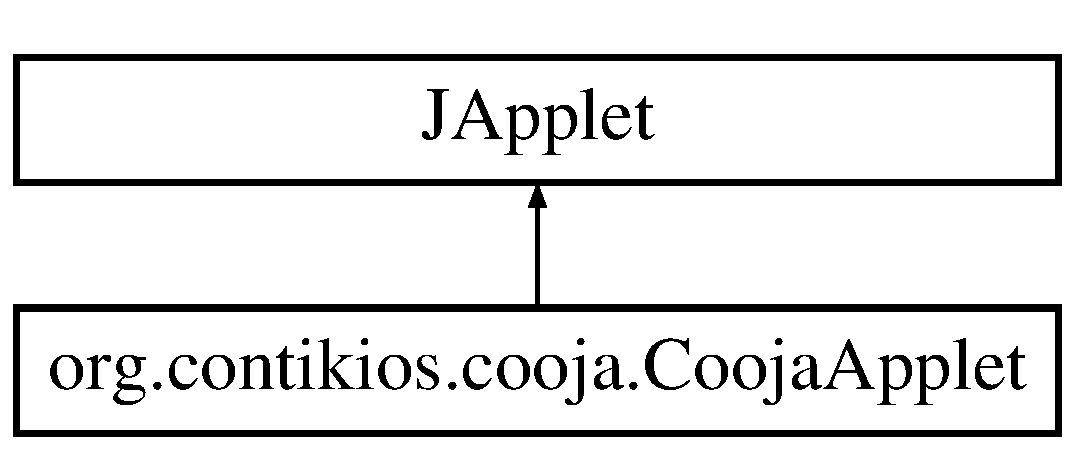
\includegraphics[height=2.000000cm]{classorg_1_1contikios_1_1cooja_1_1CoojaApplet}
\end{center}
\end{figure}
\subsection*{Public Member Functions}
\begin{DoxyCompactItemize}
\item 
\hypertarget{classorg_1_1contikios_1_1cooja_1_1CoojaApplet_abf6b23faf79a44175d19cfa2a30ec422}{void {\bfseries init} ()}\label{classorg_1_1contikios_1_1cooja_1_1CoojaApplet_abf6b23faf79a44175d19cfa2a30ec422}

\item 
\hypertarget{classorg_1_1contikios_1_1cooja_1_1CoojaApplet_a3ca680ed3ba46904685203e7427c26fb}{void {\bfseries start} ()}\label{classorg_1_1contikios_1_1cooja_1_1CoojaApplet_a3ca680ed3ba46904685203e7427c26fb}

\item 
\hypertarget{classorg_1_1contikios_1_1cooja_1_1CoojaApplet_a0b8fc2c632090032f84d3aa4470448e1}{void {\bfseries stop} ()}\label{classorg_1_1contikios_1_1cooja_1_1CoojaApplet_a0b8fc2c632090032f84d3aa4470448e1}

\end{DoxyCompactItemize}
\subsection*{Static Public Attributes}
\begin{DoxyCompactItemize}
\item 
\hypertarget{classorg_1_1contikios_1_1cooja_1_1CoojaApplet_ab6c49af9fc5cea3979fe1ad5c255e7cf}{static \hyperlink{classorg_1_1contikios_1_1cooja_1_1CoojaApplet}{Cooja\-Applet} {\bfseries applet} = null}\label{classorg_1_1contikios_1_1cooja_1_1CoojaApplet_ab6c49af9fc5cea3979fe1ad5c255e7cf}

\end{DoxyCompactItemize}


The documentation for this class was generated from the following file\-:\begin{DoxyCompactItemize}
\item 
Cooja\-Applet.\-java\end{DoxyCompactItemize}

\hypertarget{classorg_1_1contikios_1_1cooja_1_1COOJAProject}{\section{org.\-contikios.\-cooja.\-C\-O\-O\-J\-A\-Project Class Reference}
\label{classorg_1_1contikios_1_1cooja_1_1COOJAProject}\index{org.\-contikios.\-cooja.\-C\-O\-O\-J\-A\-Project@{org.\-contikios.\-cooja.\-C\-O\-O\-J\-A\-Project}}
}
\subsection*{Public Member Functions}
\begin{DoxyCompactItemize}
\item 
\hypertarget{classorg_1_1contikios_1_1cooja_1_1COOJAProject_a23651f1dcb5b825c3f2f436828f54ae5}{{\bfseries C\-O\-O\-J\-A\-Project} (File dir)}\label{classorg_1_1contikios_1_1cooja_1_1COOJAProject_a23651f1dcb5b825c3f2f436828f54ae5}

\item 
\hypertarget{classorg_1_1contikios_1_1cooja_1_1COOJAProject_aad2d9d98dd664355f95f8c9e05f67cd2}{boolean {\bfseries directory\-Exists} ()}\label{classorg_1_1contikios_1_1cooja_1_1COOJAProject_aad2d9d98dd664355f95f8c9e05f67cd2}

\item 
\hypertarget{classorg_1_1contikios_1_1cooja_1_1COOJAProject_a053cbd50039f5b3b0d3de9753d7af244}{boolean {\bfseries config\-Exists} ()}\label{classorg_1_1contikios_1_1cooja_1_1COOJAProject_a053cbd50039f5b3b0d3de9753d7af244}

\item 
\hypertarget{classorg_1_1contikios_1_1cooja_1_1COOJAProject_aabe4b5d71efd4e97c236ea3dbba929ca}{boolean {\bfseries config\-Read} ()}\label{classorg_1_1contikios_1_1cooja_1_1COOJAProject_aabe4b5d71efd4e97c236ea3dbba929ca}

\item 
\hypertarget{classorg_1_1contikios_1_1cooja_1_1COOJAProject_acd9fdb14ac54da07cd18881fa337229a}{boolean {\bfseries has\-Error} ()}\label{classorg_1_1contikios_1_1cooja_1_1COOJAProject_acd9fdb14ac54da07cd18881fa337229a}

\item 
String \hyperlink{classorg_1_1contikios_1_1cooja_1_1COOJAProject_ade6d2947ce76f481e4458cbbb39b878a}{get\-Description} ()
\item 
\hypertarget{classorg_1_1contikios_1_1cooja_1_1COOJAProject_ab21893daa8635a07bc4cba0a4c89d7a1}{String\mbox{[}$\,$\mbox{]} {\bfseries get\-Config\-Plugins} ()}\label{classorg_1_1contikios_1_1cooja_1_1COOJAProject_ab21893daa8635a07bc4cba0a4c89d7a1}

\item 
\hypertarget{classorg_1_1contikios_1_1cooja_1_1COOJAProject_a94302bfa54c5c311ee8c6df2b28f17a2}{String\mbox{[}$\,$\mbox{]} {\bfseries get\-Config\-J\-A\-Rs} ()}\label{classorg_1_1contikios_1_1cooja_1_1COOJAProject_a94302bfa54c5c311ee8c6df2b28f17a2}

\item 
\hypertarget{classorg_1_1contikios_1_1cooja_1_1COOJAProject_aa8527b7be4d2b7480f3da0a647083188}{String\mbox{[}$\,$\mbox{]} {\bfseries get\-Config\-Mote\-Types} ()}\label{classorg_1_1contikios_1_1cooja_1_1COOJAProject_aa8527b7be4d2b7480f3da0a647083188}

\item 
\hypertarget{classorg_1_1contikios_1_1cooja_1_1COOJAProject_a6ba392a4710d172b48f57dad9754e19f}{String\mbox{[}$\,$\mbox{]} {\bfseries get\-Config\-Radio\-Mediums} ()}\label{classorg_1_1contikios_1_1cooja_1_1COOJAProject_a6ba392a4710d172b48f57dad9754e19f}

\item 
\hypertarget{classorg_1_1contikios_1_1cooja_1_1COOJAProject_a9956332e0a483415862f53c0945bb1e6}{String\mbox{[}$\,$\mbox{]} {\bfseries get\-Config\-Mote\-Interfaces} ()}\label{classorg_1_1contikios_1_1cooja_1_1COOJAProject_a9956332e0a483415862f53c0945bb1e6}

\item 
\hypertarget{classorg_1_1contikios_1_1cooja_1_1COOJAProject_a130fcaa4a1bb60b5c235ce3b4411bbc6}{String\mbox{[}$\,$\mbox{]} {\bfseries get\-Config\-C\-Sources} ()}\label{classorg_1_1contikios_1_1cooja_1_1COOJAProject_a130fcaa4a1bb60b5c235ce3b4411bbc6}

\item 
\hypertarget{classorg_1_1contikios_1_1cooja_1_1COOJAProject_ab0b22d3d3b81afd44d1970186a94ea4e}{String {\bfseries to\-String} ()}\label{classorg_1_1contikios_1_1cooja_1_1COOJAProject_ab0b22d3d3b81afd44d1970186a94ea4e}

\end{DoxyCompactItemize}
\subsection*{Static Public Member Functions}
\begin{DoxyCompactItemize}
\item 
\hypertarget{classorg_1_1contikios_1_1cooja_1_1COOJAProject_aea515f7bdb1982b665a5bc338319e240}{static File\mbox{[}$\,$\mbox{]} {\bfseries sarch\-Projects} (File folder)}\label{classorg_1_1contikios_1_1cooja_1_1COOJAProject_aea515f7bdb1982b665a5bc338319e240}

\item 
\hypertarget{classorg_1_1contikios_1_1cooja_1_1COOJAProject_aa8c58b6d1dd0cb7d1b554b102168e8f0}{static File\mbox{[}$\,$\mbox{]} {\bfseries sarch\-Projects} (File folder, int depth)}\label{classorg_1_1contikios_1_1cooja_1_1COOJAProject_aa8c58b6d1dd0cb7d1b554b102168e8f0}

\end{DoxyCompactItemize}
\subsection*{Public Attributes}
\begin{DoxyCompactItemize}
\item 
\hypertarget{classorg_1_1contikios_1_1cooja_1_1COOJAProject_aa5520c83a85dcbd01f926b368e3626d8}{File {\bfseries dir} = null}\label{classorg_1_1contikios_1_1cooja_1_1COOJAProject_aa5520c83a85dcbd01f926b368e3626d8}

\item 
\hypertarget{classorg_1_1contikios_1_1cooja_1_1COOJAProject_a57e23ac14b9a810e554f749bea0b000c}{File {\bfseries config\-File} = null}\label{classorg_1_1contikios_1_1cooja_1_1COOJAProject_a57e23ac14b9a810e554f749bea0b000c}

\item 
\hypertarget{classorg_1_1contikios_1_1cooja_1_1COOJAProject_a2917471602adb953f8e92de2c8572312}{\hyperlink{classorg_1_1contikios_1_1cooja_1_1ProjectConfig}{Project\-Config} {\bfseries config} = null}\label{classorg_1_1contikios_1_1cooja_1_1COOJAProject_a2917471602adb953f8e92de2c8572312}

\end{DoxyCompactItemize}


\subsection{Detailed Description}
C\-O\-O\-J\-A Project.

\begin{DoxyAuthor}{Author}
Fredrik Osterlind 

Moritz Strübe 
\end{DoxyAuthor}


\subsection{Member Function Documentation}
\hypertarget{classorg_1_1contikios_1_1cooja_1_1COOJAProject_ade6d2947ce76f481e4458cbbb39b878a}{\index{org\-::contikios\-::cooja\-::\-C\-O\-O\-J\-A\-Project@{org\-::contikios\-::cooja\-::\-C\-O\-O\-J\-A\-Project}!get\-Description@{get\-Description}}
\index{get\-Description@{get\-Description}!org::contikios::cooja::COOJAProject@{org\-::contikios\-::cooja\-::\-C\-O\-O\-J\-A\-Project}}
\subsubsection[{get\-Description}]{\setlength{\rightskip}{0pt plus 5cm}String org.\-contikios.\-cooja.\-C\-O\-O\-J\-A\-Project.\-get\-Description (
\begin{DoxyParamCaption}
{}
\end{DoxyParamCaption}
)\hspace{0.3cm}{\ttfamily [inline]}}}\label{classorg_1_1contikios_1_1cooja_1_1COOJAProject_ade6d2947ce76f481e4458cbbb39b878a}
\begin{DoxyReturn}{Returns}
Description or null 
\end{DoxyReturn}


The documentation for this class was generated from the following file\-:\begin{DoxyCompactItemize}
\item 
C\-O\-O\-J\-A\-Project.\-java\end{DoxyCompactItemize}

\hypertarget{classorg_1_1contikios_1_1cooja_1_1COOJARadioPacket}{\section{org.\-contikios.\-cooja.\-C\-O\-O\-J\-A\-Radio\-Packet Class Reference}
\label{classorg_1_1contikios_1_1cooja_1_1COOJARadioPacket}\index{org.\-contikios.\-cooja.\-C\-O\-O\-J\-A\-Radio\-Packet@{org.\-contikios.\-cooja.\-C\-O\-O\-J\-A\-Radio\-Packet}}
}
Inheritance diagram for org.\-contikios.\-cooja.\-C\-O\-O\-J\-A\-Radio\-Packet\-:\begin{figure}[H]
\begin{center}
\leavevmode
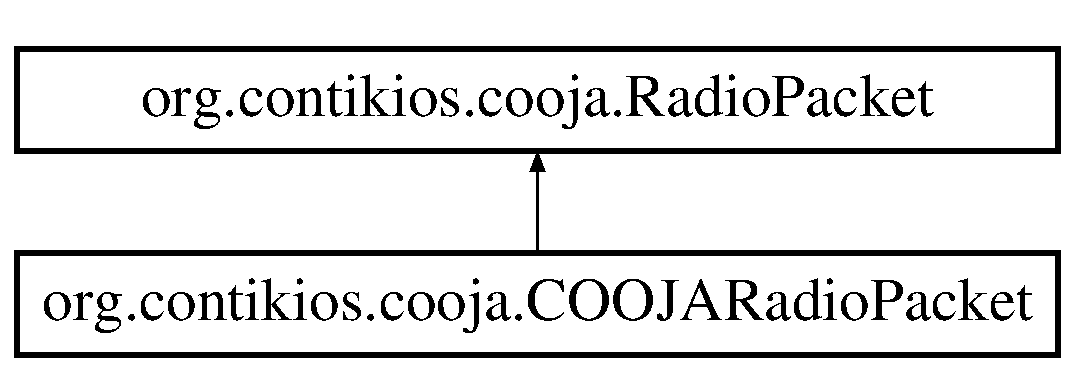
\includegraphics[height=2.000000cm]{classorg_1_1contikios_1_1cooja_1_1COOJARadioPacket}
\end{center}
\end{figure}
\subsection*{Public Member Functions}
\begin{DoxyCompactItemize}
\item 
\hypertarget{classorg_1_1contikios_1_1cooja_1_1COOJARadioPacket_ac6dd4fed045f653fbe99c9ece7f17ff3}{{\bfseries C\-O\-O\-J\-A\-Radio\-Packet} (byte\mbox{[}$\,$\mbox{]} data)}\label{classorg_1_1contikios_1_1cooja_1_1COOJARadioPacket_ac6dd4fed045f653fbe99c9ece7f17ff3}

\item 
byte\mbox{[}$\,$\mbox{]} \hyperlink{classorg_1_1contikios_1_1cooja_1_1COOJARadioPacket_a9322f1664dc941ebe8880a6530e526ff}{get\-Packet\-Data} ()
\end{DoxyCompactItemize}


\subsection{Member Function Documentation}
\hypertarget{classorg_1_1contikios_1_1cooja_1_1COOJARadioPacket_a9322f1664dc941ebe8880a6530e526ff}{\index{org\-::contikios\-::cooja\-::\-C\-O\-O\-J\-A\-Radio\-Packet@{org\-::contikios\-::cooja\-::\-C\-O\-O\-J\-A\-Radio\-Packet}!get\-Packet\-Data@{get\-Packet\-Data}}
\index{get\-Packet\-Data@{get\-Packet\-Data}!org::contikios::cooja::COOJARadioPacket@{org\-::contikios\-::cooja\-::\-C\-O\-O\-J\-A\-Radio\-Packet}}
\subsubsection[{get\-Packet\-Data}]{\setlength{\rightskip}{0pt plus 5cm}byte \mbox{[}$\,$\mbox{]} org.\-contikios.\-cooja.\-C\-O\-O\-J\-A\-Radio\-Packet.\-get\-Packet\-Data (
\begin{DoxyParamCaption}
{}
\end{DoxyParamCaption}
)\hspace{0.3cm}{\ttfamily [inline]}}}\label{classorg_1_1contikios_1_1cooja_1_1COOJARadioPacket_a9322f1664dc941ebe8880a6530e526ff}
\begin{DoxyReturn}{Returns}
Packet data 
\end{DoxyReturn}


Implements \hyperlink{interfaceorg_1_1contikios_1_1cooja_1_1RadioPacket_aaff36d4c272ded32671f47ff68253415}{org.\-contikios.\-cooja.\-Radio\-Packet}.



The documentation for this class was generated from the following file\-:\begin{DoxyCompactItemize}
\item 
C\-O\-O\-J\-A\-Radio\-Packet.\-java\end{DoxyCompactItemize}

\hypertarget{classorg_1_1contikios_1_1cooja_1_1CoreComm}{\section{org.\-contikios.\-cooja.\-Core\-Comm Class Reference}
\label{classorg_1_1contikios_1_1cooja_1_1CoreComm}\index{org.\-contikios.\-cooja.\-Core\-Comm@{org.\-contikios.\-cooja.\-Core\-Comm}}
}
\subsection*{Public Member Functions}
\begin{DoxyCompactItemize}
\item 
abstract void \hyperlink{classorg_1_1contikios_1_1cooja_1_1CoreComm_a6e6496eaaca78e77d975cfb08ebdf27f}{tick} ()
\item 
abstract void \hyperlink{classorg_1_1contikios_1_1cooja_1_1CoreComm_a684a56dd50d0c66e4111e385e09970bb}{set\-Reference\-Address} (int addr)
\item 
abstract void \hyperlink{classorg_1_1contikios_1_1cooja_1_1CoreComm_ace5ee251afbf614f27a7abe3da248d05}{get\-Memory} (int rel\-Addr, int length, byte\mbox{[}$\,$\mbox{]} mem)
\item 
abstract void \hyperlink{classorg_1_1contikios_1_1cooja_1_1CoreComm_a81682a84197a91fe8b54fe80ded9c322}{set\-Memory} (int rel\-Addr, int length, byte\mbox{[}$\,$\mbox{]} mem)
\end{DoxyCompactItemize}
\subsection*{Static Public Member Functions}
\begin{DoxyCompactItemize}
\item 
static boolean \hyperlink{classorg_1_1contikios_1_1cooja_1_1CoreComm_a213d377ca212f4d2954218b8dfc2aead}{has\-Library\-Been\-Loaded} ()
\item 
static boolean \hyperlink{classorg_1_1contikios_1_1cooja_1_1CoreComm_a45c2faad923d4f33614f6ed4e82a4a36}{has\-Library\-File\-Been\-Loaded} (File library\-File)
\item 
static String \hyperlink{classorg_1_1contikios_1_1cooja_1_1CoreComm_a2e2fa7e2f9ffa0c4827f940791680447}{get\-Available\-Class\-Name} ()
\item 
static void \hyperlink{classorg_1_1contikios_1_1cooja_1_1CoreComm_a9bf122532833fd5c093649e06950f62d}{generate\-Lib\-Source\-File} (String class\-Name)  throws Mote\-Type\-Creation\-Exception 
\item 
static void \hyperlink{classorg_1_1contikios_1_1cooja_1_1CoreComm_af6d4093df45a4bf1d22e82b4ae0a8f76}{compile\-Source\-File} (String class\-Name)  throws Mote\-Type\-Creation\-Exception 
\item 
static Class$<$?$>$ \hyperlink{classorg_1_1contikios_1_1cooja_1_1CoreComm_ab9c811edc26e54ef6cb8dfbaa54a01f1}{load\-Class\-File} (String class\-Name)  throws Mote\-Type\-Creation\-Exception 
\item 
static \hyperlink{classorg_1_1contikios_1_1cooja_1_1CoreComm}{Core\-Comm} \hyperlink{classorg_1_1contikios_1_1cooja_1_1CoreComm_a14cb8778960244ee77a6c94eb940270e}{create\-Core\-Comm} (String class\-Name, File lib\-File)  throws Mote\-Type\-Creation\-Exception 
\end{DoxyCompactItemize}
\subsection*{Protected Member Functions}
\begin{DoxyCompactItemize}
\item 
abstract void \hyperlink{classorg_1_1contikios_1_1cooja_1_1CoreComm_a50bd0205ea051af5404a2ffd44155899}{init} ()
\end{DoxyCompactItemize}


\subsection{Detailed Description}
The purpose of corecomm's is communicating with a compiled Contiki system using Java Native Interface (J\-N\-I). Each implemented class (named Lib\mbox{[}number\mbox{]}), loads a shared library which belongs to one mote type. The reason for this somewhat strange design is that once loaded, a native library cannot be unloaded in Java (in the current versions available). Therefore if we wish to load several libraries, the names and associated native functions must have unique names. And those names are defined via the calling class in J\-N\-I. For example, the corresponding function for a native tick method in class Lib1 will be named Java\-\_\-org\-\_\-contikios\-\_\-cooja\-\_\-corecomm\-\_\-\-Lib1\-\_\-tick. When creating a new mote type, the main Contiki source file is generated with function names compatible with the next available corecomm class. This also implies that even if a mote type is deleted, a new one cannot be created using the same corecomm class without restarting the J\-V\-M and thus the entire simulation.

Each implemented \hyperlink{classorg_1_1contikios_1_1cooja_1_1CoreComm}{Core\-Comm} class needs read access to the following core variables\-: 
\begin{DoxyItemize}
\item reference\-Var 
\end{DoxyItemize}and the following native functions\-: 
\begin{DoxyItemize}
\item \hyperlink{classorg_1_1contikios_1_1cooja_1_1CoreComm_a6e6496eaaca78e77d975cfb08ebdf27f}{tick()} 
\item \hyperlink{classorg_1_1contikios_1_1cooja_1_1CoreComm_a50bd0205ea051af5404a2ffd44155899}{init()} 
\item get\-Reference\-Abs\-Addr() 
\item \hyperlink{classorg_1_1contikios_1_1cooja_1_1CoreComm_ace5ee251afbf614f27a7abe3da248d05}{get\-Memory(int start, int length, byte\mbox{[}$\,$\mbox{]} mem)} 
\item \hyperlink{classorg_1_1contikios_1_1cooja_1_1CoreComm_a81682a84197a91fe8b54fe80ded9c322}{set\-Memory(int start, int length, byte\mbox{[}$\,$\mbox{]} mem)}

\begin{DoxyAuthor}{Author}
Fredrik Osterlind 
\end{DoxyAuthor}

\end{DoxyItemize}

\subsection{Member Function Documentation}
\hypertarget{classorg_1_1contikios_1_1cooja_1_1CoreComm_af6d4093df45a4bf1d22e82b4ae0a8f76}{\index{org\-::contikios\-::cooja\-::\-Core\-Comm@{org\-::contikios\-::cooja\-::\-Core\-Comm}!compile\-Source\-File@{compile\-Source\-File}}
\index{compile\-Source\-File@{compile\-Source\-File}!org::contikios::cooja::CoreComm@{org\-::contikios\-::cooja\-::\-Core\-Comm}}
\subsubsection[{compile\-Source\-File}]{\setlength{\rightskip}{0pt plus 5cm}static void org.\-contikios.\-cooja.\-Core\-Comm.\-compile\-Source\-File (
\begin{DoxyParamCaption}
\item[{String}]{class\-Name}
\end{DoxyParamCaption}
) throws Mote\-Type\-Creation\-Exception\hspace{0.3cm}{\ttfamily [inline]}, {\ttfamily [static]}}}\label{classorg_1_1contikios_1_1cooja_1_1CoreComm_af6d4093df45a4bf1d22e82b4ae0a8f76}
Compiles Java class.


\begin{DoxyParams}{Parameters}
{\em class\-Name} & Java class name (without extension) \\
\hline
\end{DoxyParams}

\begin{DoxyExceptions}{Exceptions}
{\em Mote\-Type\-Creation\-Exception} & If Java class compilation error occurs \\
\hline
\end{DoxyExceptions}
\hypertarget{classorg_1_1contikios_1_1cooja_1_1CoreComm_a14cb8778960244ee77a6c94eb940270e}{\index{org\-::contikios\-::cooja\-::\-Core\-Comm@{org\-::contikios\-::cooja\-::\-Core\-Comm}!create\-Core\-Comm@{create\-Core\-Comm}}
\index{create\-Core\-Comm@{create\-Core\-Comm}!org::contikios::cooja::CoreComm@{org\-::contikios\-::cooja\-::\-Core\-Comm}}
\subsubsection[{create\-Core\-Comm}]{\setlength{\rightskip}{0pt plus 5cm}static {\bf Core\-Comm} org.\-contikios.\-cooja.\-Core\-Comm.\-create\-Core\-Comm (
\begin{DoxyParamCaption}
\item[{String}]{class\-Name, }
\item[{File}]{lib\-File}
\end{DoxyParamCaption}
) throws Mote\-Type\-Creation\-Exception\hspace{0.3cm}{\ttfamily [inline]}, {\ttfamily [static]}}}\label{classorg_1_1contikios_1_1cooja_1_1CoreComm_a14cb8778960244ee77a6c94eb940270e}
Create and return an instance of the core communicator identified by class\-Name. This core communicator will load the native library lib\-File.


\begin{DoxyParams}{Parameters}
{\em class\-Name} & Class name of core communicator \\
\hline
{\em lib\-File} & Native library file \\
\hline
\end{DoxyParams}
\begin{DoxyReturn}{Returns}
Core Communicator 
\end{DoxyReturn}
\hypertarget{classorg_1_1contikios_1_1cooja_1_1CoreComm_a9bf122532833fd5c093649e06950f62d}{\index{org\-::contikios\-::cooja\-::\-Core\-Comm@{org\-::contikios\-::cooja\-::\-Core\-Comm}!generate\-Lib\-Source\-File@{generate\-Lib\-Source\-File}}
\index{generate\-Lib\-Source\-File@{generate\-Lib\-Source\-File}!org::contikios::cooja::CoreComm@{org\-::contikios\-::cooja\-::\-Core\-Comm}}
\subsubsection[{generate\-Lib\-Source\-File}]{\setlength{\rightskip}{0pt plus 5cm}static void org.\-contikios.\-cooja.\-Core\-Comm.\-generate\-Lib\-Source\-File (
\begin{DoxyParamCaption}
\item[{String}]{class\-Name}
\end{DoxyParamCaption}
) throws Mote\-Type\-Creation\-Exception\hspace{0.3cm}{\ttfamily [inline]}, {\ttfamily [static]}}}\label{classorg_1_1contikios_1_1cooja_1_1CoreComm_a9bf122532833fd5c093649e06950f62d}
Generates new source file by reading default source template and replacing the class name field.


\begin{DoxyParams}{Parameters}
{\em class\-Name} & Java class name (without extension) \\
\hline
\end{DoxyParams}

\begin{DoxyExceptions}{Exceptions}
{\em Mote\-Type\-Creation\-Exception} & If error occurs \\
\hline
\end{DoxyExceptions}
\hypertarget{classorg_1_1contikios_1_1cooja_1_1CoreComm_a2e2fa7e2f9ffa0c4827f940791680447}{\index{org\-::contikios\-::cooja\-::\-Core\-Comm@{org\-::contikios\-::cooja\-::\-Core\-Comm}!get\-Available\-Class\-Name@{get\-Available\-Class\-Name}}
\index{get\-Available\-Class\-Name@{get\-Available\-Class\-Name}!org::contikios::cooja::CoreComm@{org\-::contikios\-::cooja\-::\-Core\-Comm}}
\subsubsection[{get\-Available\-Class\-Name}]{\setlength{\rightskip}{0pt plus 5cm}static String org.\-contikios.\-cooja.\-Core\-Comm.\-get\-Available\-Class\-Name (
\begin{DoxyParamCaption}
{}
\end{DoxyParamCaption}
)\hspace{0.3cm}{\ttfamily [inline]}, {\ttfamily [static]}}}\label{classorg_1_1contikios_1_1cooja_1_1CoreComm_a2e2fa7e2f9ffa0c4827f940791680447}
Get the class name of next free core communicator class. If null is returned, no classes are available.

\begin{DoxyReturn}{Returns}
Class name 
\end{DoxyReturn}
\hypertarget{classorg_1_1contikios_1_1cooja_1_1CoreComm_ace5ee251afbf614f27a7abe3da248d05}{\index{org\-::contikios\-::cooja\-::\-Core\-Comm@{org\-::contikios\-::cooja\-::\-Core\-Comm}!get\-Memory@{get\-Memory}}
\index{get\-Memory@{get\-Memory}!org::contikios::cooja::CoreComm@{org\-::contikios\-::cooja\-::\-Core\-Comm}}
\subsubsection[{get\-Memory}]{\setlength{\rightskip}{0pt plus 5cm}abstract void org.\-contikios.\-cooja.\-Core\-Comm.\-get\-Memory (
\begin{DoxyParamCaption}
\item[{int}]{rel\-Addr, }
\item[{int}]{length, }
\item[{byte\mbox{[}$\,$\mbox{]}}]{mem}
\end{DoxyParamCaption}
)\hspace{0.3cm}{\ttfamily [abstract]}}}\label{classorg_1_1contikios_1_1cooja_1_1CoreComm_ace5ee251afbf614f27a7abe3da248d05}
Fills an byte array with memory segment identified by start and length.


\begin{DoxyParams}{Parameters}
{\em rel\-Addr} & Relative memory start address \\
\hline
{\em length} & Length of segment \\
\hline
{\em mem} & Array to fill with memory segment \\
\hline
\end{DoxyParams}
\hypertarget{classorg_1_1contikios_1_1cooja_1_1CoreComm_a213d377ca212f4d2954218b8dfc2aead}{\index{org\-::contikios\-::cooja\-::\-Core\-Comm@{org\-::contikios\-::cooja\-::\-Core\-Comm}!has\-Library\-Been\-Loaded@{has\-Library\-Been\-Loaded}}
\index{has\-Library\-Been\-Loaded@{has\-Library\-Been\-Loaded}!org::contikios::cooja::CoreComm@{org\-::contikios\-::cooja\-::\-Core\-Comm}}
\subsubsection[{has\-Library\-Been\-Loaded}]{\setlength{\rightskip}{0pt plus 5cm}static boolean org.\-contikios.\-cooja.\-Core\-Comm.\-has\-Library\-Been\-Loaded (
\begin{DoxyParamCaption}
{}
\end{DoxyParamCaption}
)\hspace{0.3cm}{\ttfamily [inline]}, {\ttfamily [static]}}}\label{classorg_1_1contikios_1_1cooja_1_1CoreComm_a213d377ca212f4d2954218b8dfc2aead}
Has any library been loaded? Since libraries can't be unloaded the entire simulator may have to be restarted.

\begin{DoxyReturn}{Returns}
True if any library has been loaded this session 
\end{DoxyReturn}
\hypertarget{classorg_1_1contikios_1_1cooja_1_1CoreComm_a45c2faad923d4f33614f6ed4e82a4a36}{\index{org\-::contikios\-::cooja\-::\-Core\-Comm@{org\-::contikios\-::cooja\-::\-Core\-Comm}!has\-Library\-File\-Been\-Loaded@{has\-Library\-File\-Been\-Loaded}}
\index{has\-Library\-File\-Been\-Loaded@{has\-Library\-File\-Been\-Loaded}!org::contikios::cooja::CoreComm@{org\-::contikios\-::cooja\-::\-Core\-Comm}}
\subsubsection[{has\-Library\-File\-Been\-Loaded}]{\setlength{\rightskip}{0pt plus 5cm}static boolean org.\-contikios.\-cooja.\-Core\-Comm.\-has\-Library\-File\-Been\-Loaded (
\begin{DoxyParamCaption}
\item[{File}]{library\-File}
\end{DoxyParamCaption}
)\hspace{0.3cm}{\ttfamily [inline]}, {\ttfamily [static]}}}\label{classorg_1_1contikios_1_1cooja_1_1CoreComm_a45c2faad923d4f33614f6ed4e82a4a36}
Has given library file already been loaded during this session? A loaded library can be removed, but not unloaded during one session. And a new library file, named the same as an earlier loaded and removed file, can't be loaded either.


\begin{DoxyParams}{Parameters}
{\em library\-File} & Library file \\
\hline
\end{DoxyParams}
\begin{DoxyReturn}{Returns}
True if a library has already been loaded from the given file's filename 
\end{DoxyReturn}
\hypertarget{classorg_1_1contikios_1_1cooja_1_1CoreComm_a50bd0205ea051af5404a2ffd44155899}{\index{org\-::contikios\-::cooja\-::\-Core\-Comm@{org\-::contikios\-::cooja\-::\-Core\-Comm}!init@{init}}
\index{init@{init}!org::contikios::cooja::CoreComm@{org\-::contikios\-::cooja\-::\-Core\-Comm}}
\subsubsection[{init}]{\setlength{\rightskip}{0pt plus 5cm}abstract void org.\-contikios.\-cooja.\-Core\-Comm.\-init (
\begin{DoxyParamCaption}
{}
\end{DoxyParamCaption}
)\hspace{0.3cm}{\ttfamily [abstract]}, {\ttfamily [protected]}}}\label{classorg_1_1contikios_1_1cooja_1_1CoreComm_a50bd0205ea051af5404a2ffd44155899}
Initializes a mote by running a startup script in the core. (Should only be run once, at the same time as the library is loaded) \hypertarget{classorg_1_1contikios_1_1cooja_1_1CoreComm_ab9c811edc26e54ef6cb8dfbaa54a01f1}{\index{org\-::contikios\-::cooja\-::\-Core\-Comm@{org\-::contikios\-::cooja\-::\-Core\-Comm}!load\-Class\-File@{load\-Class\-File}}
\index{load\-Class\-File@{load\-Class\-File}!org::contikios::cooja::CoreComm@{org\-::contikios\-::cooja\-::\-Core\-Comm}}
\subsubsection[{load\-Class\-File}]{\setlength{\rightskip}{0pt plus 5cm}static Class$<$?$>$ org.\-contikios.\-cooja.\-Core\-Comm.\-load\-Class\-File (
\begin{DoxyParamCaption}
\item[{String}]{class\-Name}
\end{DoxyParamCaption}
) throws Mote\-Type\-Creation\-Exception\hspace{0.3cm}{\ttfamily [inline]}, {\ttfamily [static]}}}\label{classorg_1_1contikios_1_1cooja_1_1CoreComm_ab9c811edc26e54ef6cb8dfbaa54a01f1}
Loads given Java class file from disk.


\begin{DoxyParams}{Parameters}
{\em class\-Name} & Java class name \\
\hline
\end{DoxyParams}
\begin{DoxyReturn}{Returns}
Loaded class 
\end{DoxyReturn}

\begin{DoxyExceptions}{Exceptions}
{\em Mote\-Type\-Creation\-Exception} & If error occurs \\
\hline
\end{DoxyExceptions}
\hypertarget{classorg_1_1contikios_1_1cooja_1_1CoreComm_a81682a84197a91fe8b54fe80ded9c322}{\index{org\-::contikios\-::cooja\-::\-Core\-Comm@{org\-::contikios\-::cooja\-::\-Core\-Comm}!set\-Memory@{set\-Memory}}
\index{set\-Memory@{set\-Memory}!org::contikios::cooja::CoreComm@{org\-::contikios\-::cooja\-::\-Core\-Comm}}
\subsubsection[{set\-Memory}]{\setlength{\rightskip}{0pt plus 5cm}abstract void org.\-contikios.\-cooja.\-Core\-Comm.\-set\-Memory (
\begin{DoxyParamCaption}
\item[{int}]{rel\-Addr, }
\item[{int}]{length, }
\item[{byte\mbox{[}$\,$\mbox{]}}]{mem}
\end{DoxyParamCaption}
)\hspace{0.3cm}{\ttfamily [abstract]}}}\label{classorg_1_1contikios_1_1cooja_1_1CoreComm_a81682a84197a91fe8b54fe80ded9c322}
Overwrites a memory segment identified by start and length.


\begin{DoxyParams}{Parameters}
{\em rel\-Addr} & Relative memory start address \\
\hline
{\em length} & Length of segment \\
\hline
{\em mem} & New memory segment data \\
\hline
\end{DoxyParams}
\hypertarget{classorg_1_1contikios_1_1cooja_1_1CoreComm_a684a56dd50d0c66e4111e385e09970bb}{\index{org\-::contikios\-::cooja\-::\-Core\-Comm@{org\-::contikios\-::cooja\-::\-Core\-Comm}!set\-Reference\-Address@{set\-Reference\-Address}}
\index{set\-Reference\-Address@{set\-Reference\-Address}!org::contikios::cooja::CoreComm@{org\-::contikios\-::cooja\-::\-Core\-Comm}}
\subsubsection[{set\-Reference\-Address}]{\setlength{\rightskip}{0pt plus 5cm}abstract void org.\-contikios.\-cooja.\-Core\-Comm.\-set\-Reference\-Address (
\begin{DoxyParamCaption}
\item[{int}]{addr}
\end{DoxyParamCaption}
)\hspace{0.3cm}{\ttfamily [abstract]}}}\label{classorg_1_1contikios_1_1cooja_1_1CoreComm_a684a56dd50d0c66e4111e385e09970bb}
Sets the relative memory address of the reference variable. Is used by Contiki to map between absolute and relative memory addresses.


\begin{DoxyParams}{Parameters}
{\em addr} & Relative address \\
\hline
\end{DoxyParams}
\hypertarget{classorg_1_1contikios_1_1cooja_1_1CoreComm_a6e6496eaaca78e77d975cfb08ebdf27f}{\index{org\-::contikios\-::cooja\-::\-Core\-Comm@{org\-::contikios\-::cooja\-::\-Core\-Comm}!tick@{tick}}
\index{tick@{tick}!org::contikios::cooja::CoreComm@{org\-::contikios\-::cooja\-::\-Core\-Comm}}
\subsubsection[{tick}]{\setlength{\rightskip}{0pt plus 5cm}abstract void org.\-contikios.\-cooja.\-Core\-Comm.\-tick (
\begin{DoxyParamCaption}
{}
\end{DoxyParamCaption}
)\hspace{0.3cm}{\ttfamily [abstract]}}}\label{classorg_1_1contikios_1_1cooja_1_1CoreComm_a6e6496eaaca78e77d975cfb08ebdf27f}
Ticks a mote once. This should not be used directly, but instead via \hyperlink{}{Contiki\-Mote\-Type\#tick()}. 

The documentation for this class was generated from the following file\-:\begin{DoxyCompactItemize}
\item 
Core\-Comm.\-java\end{DoxyCompactItemize}

\hypertarget{classorg_1_1contikios_1_1cooja_1_1EventQueue}{\section{org.\-contikios.\-cooja.\-Event\-Queue Class Reference}
\label{classorg_1_1contikios_1_1cooja_1_1EventQueue}\index{org.\-contikios.\-cooja.\-Event\-Queue@{org.\-contikios.\-cooja.\-Event\-Queue}}
}
\subsection*{Public Member Functions}
\begin{DoxyCompactItemize}
\item 
void \hyperlink{classorg_1_1contikios_1_1cooja_1_1EventQueue_af77e94c75d1e897329585af90d63a228}{add\-Event} (\hyperlink{classorg_1_1contikios_1_1cooja_1_1TimeEvent}{Time\-Event} event, long time)
\item 
\hypertarget{classorg_1_1contikios_1_1cooja_1_1EventQueue_a133265d84748cad8ba08f8dc06e00362}{void {\bfseries remove\-All} ()}\label{classorg_1_1contikios_1_1cooja_1_1EventQueue_a133265d84748cad8ba08f8dc06e00362}

\item 
\hyperlink{classorg_1_1contikios_1_1cooja_1_1TimeEvent}{Time\-Event} \hyperlink{classorg_1_1contikios_1_1cooja_1_1EventQueue_a44f7ce071f5e541415e061964b3f17fd}{pop\-First} ()
\item 
\hypertarget{classorg_1_1contikios_1_1cooja_1_1EventQueue_a781f17b00625d93f939e7dd3ed5eb27a}{\hyperlink{classorg_1_1contikios_1_1cooja_1_1TimeEvent}{Time\-Event} {\bfseries peek\-First} ()}\label{classorg_1_1contikios_1_1cooja_1_1EventQueue_a781f17b00625d93f939e7dd3ed5eb27a}

\item 
\hypertarget{classorg_1_1contikios_1_1cooja_1_1EventQueue_a835b2c652959b915e995b49d94f78b39}{String {\bfseries to\-String} ()}\label{classorg_1_1contikios_1_1cooja_1_1EventQueue_a835b2c652959b915e995b49d94f78b39}

\end{DoxyCompactItemize}


\subsection{Detailed Description}
\begin{DoxyAuthor}{Author}
Joakim Eriksson (ported to C\-O\-O\-J\-A by Fredrik Osterlind) 
\end{DoxyAuthor}


\subsection{Member Function Documentation}
\hypertarget{classorg_1_1contikios_1_1cooja_1_1EventQueue_af77e94c75d1e897329585af90d63a228}{\index{org\-::contikios\-::cooja\-::\-Event\-Queue@{org\-::contikios\-::cooja\-::\-Event\-Queue}!add\-Event@{add\-Event}}
\index{add\-Event@{add\-Event}!org::contikios::cooja::EventQueue@{org\-::contikios\-::cooja\-::\-Event\-Queue}}
\subsubsection[{add\-Event}]{\setlength{\rightskip}{0pt plus 5cm}void org.\-contikios.\-cooja.\-Event\-Queue.\-add\-Event (
\begin{DoxyParamCaption}
\item[{{\bf Time\-Event}}]{event, }
\item[{long}]{time}
\end{DoxyParamCaption}
)\hspace{0.3cm}{\ttfamily [inline]}}}\label{classorg_1_1contikios_1_1cooja_1_1EventQueue_af77e94c75d1e897329585af90d63a228}
Should only be called from simulation thread!


\begin{DoxyParams}{Parameters}
{\em event} & Event \\
\hline
{\em time} & Time \\
\hline
\end{DoxyParams}
\hypertarget{classorg_1_1contikios_1_1cooja_1_1EventQueue_a44f7ce071f5e541415e061964b3f17fd}{\index{org\-::contikios\-::cooja\-::\-Event\-Queue@{org\-::contikios\-::cooja\-::\-Event\-Queue}!pop\-First@{pop\-First}}
\index{pop\-First@{pop\-First}!org::contikios::cooja::EventQueue@{org\-::contikios\-::cooja\-::\-Event\-Queue}}
\subsubsection[{pop\-First}]{\setlength{\rightskip}{0pt plus 5cm}{\bf Time\-Event} org.\-contikios.\-cooja.\-Event\-Queue.\-pop\-First (
\begin{DoxyParamCaption}
{}
\end{DoxyParamCaption}
)\hspace{0.3cm}{\ttfamily [inline]}}}\label{classorg_1_1contikios_1_1cooja_1_1EventQueue_a44f7ce071f5e541415e061964b3f17fd}
Should only be called from simulation thread!

\begin{DoxyReturn}{Returns}
Event 
\end{DoxyReturn}


The documentation for this class was generated from the following file\-:\begin{DoxyCompactItemize}
\item 
Event\-Queue.\-java\end{DoxyCompactItemize}

\hypertarget{classGraphicObject}{\section{Graphic\-Object Class Reference}
\label{classGraphicObject}\index{Graphic\-Object@{Graphic\-Object}}
}


The documentation for this class was generated from the following file\-:\begin{DoxyCompactItemize}
\item 
Graphic\-Object.\-java\end{DoxyCompactItemize}

\hypertarget{interfaceorg_1_1contikios_1_1cooja_1_1HasQuickHelp}{\section{org.\-contikios.\-cooja.\-Has\-Quick\-Help Interface Reference}
\label{interfaceorg_1_1contikios_1_1cooja_1_1HasQuickHelp}\index{org.\-contikios.\-cooja.\-Has\-Quick\-Help@{org.\-contikios.\-cooja.\-Has\-Quick\-Help}}
}
\subsection*{Public Member Functions}
\begin{DoxyCompactItemize}
\item 
String \hyperlink{interfaceorg_1_1contikios_1_1cooja_1_1HasQuickHelp_ae9473c143ac245fef00f8afd71ed7006}{get\-Quick\-Help} ()
\end{DoxyCompactItemize}


\subsection{Member Function Documentation}
\hypertarget{interfaceorg_1_1contikios_1_1cooja_1_1HasQuickHelp_ae9473c143ac245fef00f8afd71ed7006}{\index{org\-::contikios\-::cooja\-::\-Has\-Quick\-Help@{org\-::contikios\-::cooja\-::\-Has\-Quick\-Help}!get\-Quick\-Help@{get\-Quick\-Help}}
\index{get\-Quick\-Help@{get\-Quick\-Help}!org::contikios::cooja::HasQuickHelp@{org\-::contikios\-::cooja\-::\-Has\-Quick\-Help}}
\subsubsection[{get\-Quick\-Help}]{\setlength{\rightskip}{0pt plus 5cm}String org.\-contikios.\-cooja.\-Has\-Quick\-Help.\-get\-Quick\-Help (
\begin{DoxyParamCaption}
{}
\end{DoxyParamCaption}
)}}\label{interfaceorg_1_1contikios_1_1cooja_1_1HasQuickHelp_ae9473c143ac245fef00f8afd71ed7006}
\begin{DoxyReturn}{Returns}
Quick help. May be H\-T\-M\-L formatted, but must not include the document html-\/tags. 
\end{DoxyReturn}


The documentation for this interface was generated from the following file\-:\begin{DoxyCompactItemize}
\item 
Has\-Quick\-Help.\-java\end{DoxyCompactItemize}

\hypertarget{interfaceorg_1_1contikios_1_1cooja_1_1SimEventCentral_1_1LogOutputListener}{\section{org.\-contikios.\-cooja.\-Sim\-Event\-Central.\-Log\-Output\-Listener Interface Reference}
\label{interfaceorg_1_1contikios_1_1cooja_1_1SimEventCentral_1_1LogOutputListener}\index{org.\-contikios.\-cooja.\-Sim\-Event\-Central.\-Log\-Output\-Listener@{org.\-contikios.\-cooja.\-Sim\-Event\-Central.\-Log\-Output\-Listener}}
}
Inheritance diagram for org.\-contikios.\-cooja.\-Sim\-Event\-Central.\-Log\-Output\-Listener\-:\begin{figure}[H]
\begin{center}
\leavevmode
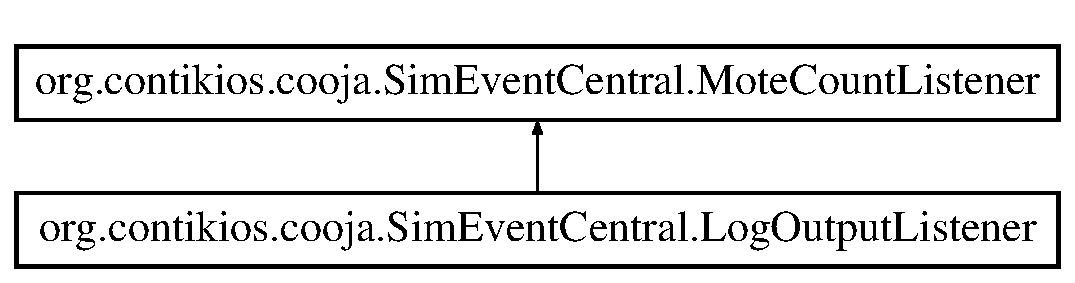
\includegraphics[height=2.000000cm]{interfaceorg_1_1contikios_1_1cooja_1_1SimEventCentral_1_1LogOutputListener}
\end{center}
\end{figure}
\subsection*{Public Member Functions}
\begin{DoxyCompactItemize}
\item 
\hypertarget{interfaceorg_1_1contikios_1_1cooja_1_1SimEventCentral_1_1LogOutputListener_ab8e50a8b0e8fd8e20b9c9efdcb69cff5}{void {\bfseries removed\-Log\-Output} (Log\-Output\-Event ev)}\label{interfaceorg_1_1contikios_1_1cooja_1_1SimEventCentral_1_1LogOutputListener_ab8e50a8b0e8fd8e20b9c9efdcb69cff5}

\item 
\hypertarget{interfaceorg_1_1contikios_1_1cooja_1_1SimEventCentral_1_1LogOutputListener_a714c9a39742d1e8f6aee7a4dc9f62e0c}{void {\bfseries new\-Log\-Output} (Log\-Output\-Event ev)}\label{interfaceorg_1_1contikios_1_1cooja_1_1SimEventCentral_1_1LogOutputListener_a714c9a39742d1e8f6aee7a4dc9f62e0c}

\end{DoxyCompactItemize}


The documentation for this interface was generated from the following file\-:\begin{DoxyCompactItemize}
\item 
Sim\-Event\-Central.\-java\end{DoxyCompactItemize}

\hypertarget{interfaceorg_1_1contikios_1_1cooja_1_1Mote}{\section{org.\-contikios.\-cooja.\-Mote Interface Reference}
\label{interfaceorg_1_1contikios_1_1cooja_1_1Mote}\index{org.\-contikios.\-cooja.\-Mote@{org.\-contikios.\-cooja.\-Mote}}
}
Inheritance diagram for org.\-contikios.\-cooja.\-Mote\-:\begin{figure}[H]
\begin{center}
\leavevmode
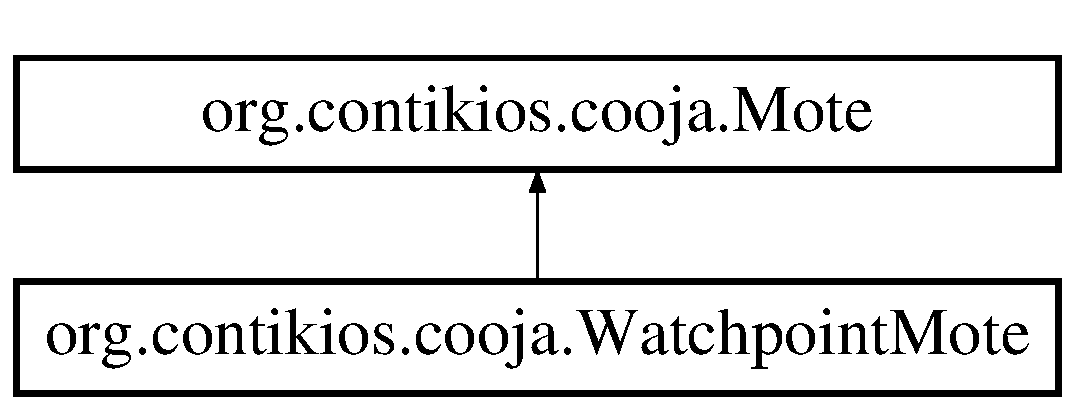
\includegraphics[height=2.000000cm]{interfaceorg_1_1contikios_1_1cooja_1_1Mote}
\end{center}
\end{figure}
\subsection*{Public Member Functions}
\begin{DoxyCompactItemize}
\item 
int \hyperlink{interfaceorg_1_1contikios_1_1cooja_1_1Mote_ace9d66ac50f3dba7ae725a16a8172aa6}{get\-I\-D} ()
\item 
\hyperlink{classorg_1_1contikios_1_1cooja_1_1MoteInterfaceHandler}{Mote\-Interface\-Handler} \hyperlink{interfaceorg_1_1contikios_1_1cooja_1_1Mote_a37bc264ef32cdd78b2b126d83e7a42d4}{get\-Interfaces} ()
\item 
Memory\-Interface \hyperlink{interfaceorg_1_1contikios_1_1cooja_1_1Mote_a239aebd679450f6face2073f0599a13f}{get\-Memory} ()
\item 
\hyperlink{interfaceorg_1_1contikios_1_1cooja_1_1MoteType}{Mote\-Type} \hyperlink{interfaceorg_1_1contikios_1_1cooja_1_1Mote_ab8120b25191f1101e79f1986ac90639c}{get\-Type} ()
\item 
\hyperlink{classorg_1_1contikios_1_1cooja_1_1Simulation}{Simulation} \hyperlink{interfaceorg_1_1contikios_1_1cooja_1_1Mote_abda92c72b3264208f6d3c1deb7cc6a6e}{get\-Simulation} ()
\item 
abstract Collection$<$ Element $>$ \hyperlink{interfaceorg_1_1contikios_1_1cooja_1_1Mote_a588f56dddb96a6f996ebe99264e4cba3}{get\-Config\-X\-M\-L} ()
\item 
abstract boolean \hyperlink{interfaceorg_1_1contikios_1_1cooja_1_1Mote_afd2320eec3cd8dc02f80286b40f1ad3a}{set\-Config\-X\-M\-L} (\hyperlink{classorg_1_1contikios_1_1cooja_1_1Simulation}{Simulation} simulation, Collection$<$ Element $>$ config\-X\-M\-L, boolean vis\-Available)
\item 
void \hyperlink{interfaceorg_1_1contikios_1_1cooja_1_1Mote_a03fcd439ae5bec154da6146925971f28}{removed} ()
\item 
\hypertarget{interfaceorg_1_1contikios_1_1cooja_1_1Mote_ad8d19948b08e53093123aff13c3e4e49}{void {\bfseries set\-Property} (String key, Object obj)}\label{interfaceorg_1_1contikios_1_1cooja_1_1Mote_ad8d19948b08e53093123aff13c3e4e49}

\item 
\hypertarget{interfaceorg_1_1contikios_1_1cooja_1_1Mote_a28c82cca6413b812bc8e815a30f8041d}{Object {\bfseries get\-Property} (String key)}\label{interfaceorg_1_1contikios_1_1cooja_1_1Mote_a28c82cca6413b812bc8e815a30f8041d}

\end{DoxyCompactItemize}


\subsection{Detailed Description}
A simulated mote.

All motes have an interface handler, a mote type and a mote memory.

\begin{DoxySeeAlso}{See Also}
\hyperlink{classorg_1_1contikios_1_1cooja_1_1MoteInterfaceHandler}{org.\-contikios.\-cooja.\-Mote\-Interface\-Handler} 

org.\-contikios.\-cooja.\-Mote\-Memory 

\hyperlink{interfaceorg_1_1contikios_1_1cooja_1_1MoteType}{org.\-contikios.\-cooja.\-Mote\-Type}
\end{DoxySeeAlso}
\begin{DoxyAuthor}{Author}
Fredrik Osterlind 
\end{DoxyAuthor}


\subsection{Member Function Documentation}
\hypertarget{interfaceorg_1_1contikios_1_1cooja_1_1Mote_a588f56dddb96a6f996ebe99264e4cba3}{\index{org\-::contikios\-::cooja\-::\-Mote@{org\-::contikios\-::cooja\-::\-Mote}!get\-Config\-X\-M\-L@{get\-Config\-X\-M\-L}}
\index{get\-Config\-X\-M\-L@{get\-Config\-X\-M\-L}!org::contikios::cooja::Mote@{org\-::contikios\-::cooja\-::\-Mote}}
\subsubsection[{get\-Config\-X\-M\-L}]{\setlength{\rightskip}{0pt plus 5cm}abstract Collection$<$Element$>$ org.\-contikios.\-cooja.\-Mote.\-get\-Config\-X\-M\-L (
\begin{DoxyParamCaption}
{}
\end{DoxyParamCaption}
)\hspace{0.3cm}{\ttfamily [abstract]}}}\label{interfaceorg_1_1contikios_1_1cooja_1_1Mote_a588f56dddb96a6f996ebe99264e4cba3}
Returns X\-M\-L elements representing the current config of this mote. This is fetched by the simulator for example when saving a simulation configuration file. For example a mote may return the configs of all its interfaces. This method should however not return state specific information. (All nodes are restarted when loading a simulation.)

\begin{DoxySeeAlso}{See Also}
\#set\-Config\-X\-M\-L(\-Simulation, Collection, boolean) 
\end{DoxySeeAlso}
\begin{DoxyReturn}{Returns}
X\-M\-L elements representing the current mote config 
\end{DoxyReturn}
\hypertarget{interfaceorg_1_1contikios_1_1cooja_1_1Mote_ace9d66ac50f3dba7ae725a16a8172aa6}{\index{org\-::contikios\-::cooja\-::\-Mote@{org\-::contikios\-::cooja\-::\-Mote}!get\-I\-D@{get\-I\-D}}
\index{get\-I\-D@{get\-I\-D}!org::contikios::cooja::Mote@{org\-::contikios\-::cooja\-::\-Mote}}
\subsubsection[{get\-I\-D}]{\setlength{\rightskip}{0pt plus 5cm}int org.\-contikios.\-cooja.\-Mote.\-get\-I\-D (
\begin{DoxyParamCaption}
{}
\end{DoxyParamCaption}
)}}\label{interfaceorg_1_1contikios_1_1cooja_1_1Mote_ace9d66ac50f3dba7ae725a16a8172aa6}
\begin{DoxyReturn}{Returns}
Unique mote I\-D 
\end{DoxyReturn}
\hypertarget{interfaceorg_1_1contikios_1_1cooja_1_1Mote_a37bc264ef32cdd78b2b126d83e7a42d4}{\index{org\-::contikios\-::cooja\-::\-Mote@{org\-::contikios\-::cooja\-::\-Mote}!get\-Interfaces@{get\-Interfaces}}
\index{get\-Interfaces@{get\-Interfaces}!org::contikios::cooja::Mote@{org\-::contikios\-::cooja\-::\-Mote}}
\subsubsection[{get\-Interfaces}]{\setlength{\rightskip}{0pt plus 5cm}{\bf Mote\-Interface\-Handler} org.\-contikios.\-cooja.\-Mote.\-get\-Interfaces (
\begin{DoxyParamCaption}
{}
\end{DoxyParamCaption}
)}}\label{interfaceorg_1_1contikios_1_1cooja_1_1Mote_a37bc264ef32cdd78b2b126d83e7a42d4}
Returns the interface handler of this mote.

\begin{DoxySeeAlso}{See Also}
\#set\-Interfaces(\-Mote\-Interface\-Handler) 
\end{DoxySeeAlso}
\begin{DoxyReturn}{Returns}
\hyperlink{interfaceorg_1_1contikios_1_1cooja_1_1Mote}{Mote} interface handler 
\end{DoxyReturn}
\hypertarget{interfaceorg_1_1contikios_1_1cooja_1_1Mote_a239aebd679450f6face2073f0599a13f}{\index{org\-::contikios\-::cooja\-::\-Mote@{org\-::contikios\-::cooja\-::\-Mote}!get\-Memory@{get\-Memory}}
\index{get\-Memory@{get\-Memory}!org::contikios::cooja::Mote@{org\-::contikios\-::cooja\-::\-Mote}}
\subsubsection[{get\-Memory}]{\setlength{\rightskip}{0pt plus 5cm}Memory\-Interface org.\-contikios.\-cooja.\-Mote.\-get\-Memory (
\begin{DoxyParamCaption}
{}
\end{DoxyParamCaption}
)}}\label{interfaceorg_1_1contikios_1_1cooja_1_1Mote_a239aebd679450f6face2073f0599a13f}
Returns the memory of this mote.

\begin{DoxySeeAlso}{See Also}
\#set\-Memory(\-Mote\-Memory) 
\end{DoxySeeAlso}
\begin{DoxyReturn}{Returns}
\hyperlink{interfaceorg_1_1contikios_1_1cooja_1_1Mote}{Mote} memory 
\end{DoxyReturn}
\hypertarget{interfaceorg_1_1contikios_1_1cooja_1_1Mote_abda92c72b3264208f6d3c1deb7cc6a6e}{\index{org\-::contikios\-::cooja\-::\-Mote@{org\-::contikios\-::cooja\-::\-Mote}!get\-Simulation@{get\-Simulation}}
\index{get\-Simulation@{get\-Simulation}!org::contikios::cooja::Mote@{org\-::contikios\-::cooja\-::\-Mote}}
\subsubsection[{get\-Simulation}]{\setlength{\rightskip}{0pt plus 5cm}{\bf Simulation} org.\-contikios.\-cooja.\-Mote.\-get\-Simulation (
\begin{DoxyParamCaption}
{}
\end{DoxyParamCaption}
)}}\label{interfaceorg_1_1contikios_1_1cooja_1_1Mote_abda92c72b3264208f6d3c1deb7cc6a6e}
Returns simulation which holds this mote.

\begin{DoxySeeAlso}{See Also}
\#set\-Simulation(\-Simulation) 
\end{DoxySeeAlso}
\begin{DoxyReturn}{Returns}
\hyperlink{classorg_1_1contikios_1_1cooja_1_1Simulation}{Simulation} 
\end{DoxyReturn}
\hypertarget{interfaceorg_1_1contikios_1_1cooja_1_1Mote_ab8120b25191f1101e79f1986ac90639c}{\index{org\-::contikios\-::cooja\-::\-Mote@{org\-::contikios\-::cooja\-::\-Mote}!get\-Type@{get\-Type}}
\index{get\-Type@{get\-Type}!org::contikios::cooja::Mote@{org\-::contikios\-::cooja\-::\-Mote}}
\subsubsection[{get\-Type}]{\setlength{\rightskip}{0pt plus 5cm}{\bf Mote\-Type} org.\-contikios.\-cooja.\-Mote.\-get\-Type (
\begin{DoxyParamCaption}
{}
\end{DoxyParamCaption}
)}}\label{interfaceorg_1_1contikios_1_1cooja_1_1Mote_ab8120b25191f1101e79f1986ac90639c}
Returns mote type.

\begin{DoxySeeAlso}{See Also}
\#set\-Type(\-Mote\-Type) 
\end{DoxySeeAlso}
\begin{DoxyReturn}{Returns}
\hyperlink{interfaceorg_1_1contikios_1_1cooja_1_1Mote}{Mote} type 
\end{DoxyReturn}
\hypertarget{interfaceorg_1_1contikios_1_1cooja_1_1Mote_a03fcd439ae5bec154da6146925971f28}{\index{org\-::contikios\-::cooja\-::\-Mote@{org\-::contikios\-::cooja\-::\-Mote}!removed@{removed}}
\index{removed@{removed}!org::contikios::cooja::Mote@{org\-::contikios\-::cooja\-::\-Mote}}
\subsubsection[{removed}]{\setlength{\rightskip}{0pt plus 5cm}void org.\-contikios.\-cooja.\-Mote.\-removed (
\begin{DoxyParamCaption}
{}
\end{DoxyParamCaption}
)}}\label{interfaceorg_1_1contikios_1_1cooja_1_1Mote_a03fcd439ae5bec154da6146925971f28}
Called when mote is removed from simulation \hypertarget{interfaceorg_1_1contikios_1_1cooja_1_1Mote_afd2320eec3cd8dc02f80286b40f1ad3a}{\index{org\-::contikios\-::cooja\-::\-Mote@{org\-::contikios\-::cooja\-::\-Mote}!set\-Config\-X\-M\-L@{set\-Config\-X\-M\-L}}
\index{set\-Config\-X\-M\-L@{set\-Config\-X\-M\-L}!org::contikios::cooja::Mote@{org\-::contikios\-::cooja\-::\-Mote}}
\subsubsection[{set\-Config\-X\-M\-L}]{\setlength{\rightskip}{0pt plus 5cm}abstract boolean org.\-contikios.\-cooja.\-Mote.\-set\-Config\-X\-M\-L (
\begin{DoxyParamCaption}
\item[{{\bf Simulation}}]{simulation, }
\item[{Collection$<$ Element $>$}]{config\-X\-M\-L, }
\item[{boolean}]{vis\-Available}
\end{DoxyParamCaption}
)\hspace{0.3cm}{\ttfamily [abstract]}}}\label{interfaceorg_1_1contikios_1_1cooja_1_1Mote_afd2320eec3cd8dc02f80286b40f1ad3a}
Sets the current mote config depending on the given X\-M\-L elements.


\begin{DoxyParams}{Parameters}
{\em simulation} & \hyperlink{classorg_1_1contikios_1_1cooja_1_1Simulation}{Simulation} holding this mote \\
\hline
{\em config\-X\-M\-L} & Config X\-M\-L elements\\
\hline
\end{DoxyParams}
\begin{DoxySeeAlso}{See Also}
\hyperlink{interfaceorg_1_1contikios_1_1cooja_1_1Mote_a588f56dddb96a6f996ebe99264e4cba3}{get\-Config\-X\-M\-L()} 
\end{DoxySeeAlso}


The documentation for this interface was generated from the following file\-:\begin{DoxyCompactItemize}
\item 
Mote.\-java\end{DoxyCompactItemize}

\hypertarget{interfaceorg_1_1contikios_1_1cooja_1_1SimEventCentral_1_1MoteCountListener}{\section{org.\-contikios.\-cooja.\-Sim\-Event\-Central.\-Mote\-Count\-Listener Interface Reference}
\label{interfaceorg_1_1contikios_1_1cooja_1_1SimEventCentral_1_1MoteCountListener}\index{org.\-contikios.\-cooja.\-Sim\-Event\-Central.\-Mote\-Count\-Listener@{org.\-contikios.\-cooja.\-Sim\-Event\-Central.\-Mote\-Count\-Listener}}
}
Inheritance diagram for org.\-contikios.\-cooja.\-Sim\-Event\-Central.\-Mote\-Count\-Listener\-:\begin{figure}[H]
\begin{center}
\leavevmode
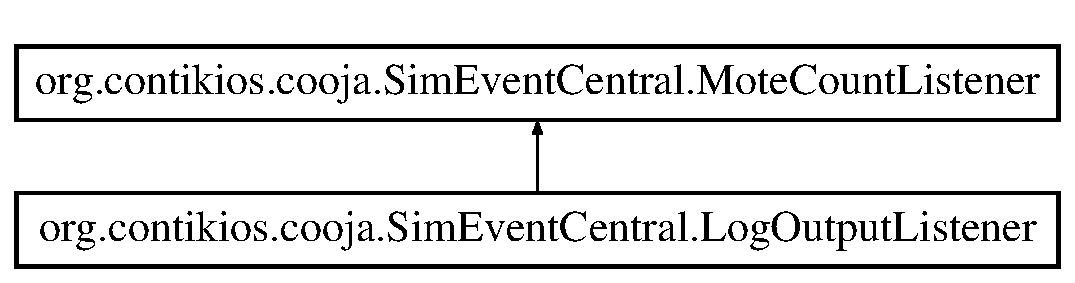
\includegraphics[height=2.000000cm]{interfaceorg_1_1contikios_1_1cooja_1_1SimEventCentral_1_1MoteCountListener}
\end{center}
\end{figure}
\subsection*{Public Member Functions}
\begin{DoxyCompactItemize}
\item 
\hypertarget{interfaceorg_1_1contikios_1_1cooja_1_1SimEventCentral_1_1MoteCountListener_a7ddd29e4abb2cabd7048ec9e8324fdf8}{void {\bfseries mote\-Was\-Added} (\hyperlink{interfaceorg_1_1contikios_1_1cooja_1_1Mote}{Mote} mote)}\label{interfaceorg_1_1contikios_1_1cooja_1_1SimEventCentral_1_1MoteCountListener_a7ddd29e4abb2cabd7048ec9e8324fdf8}

\item 
\hypertarget{interfaceorg_1_1contikios_1_1cooja_1_1SimEventCentral_1_1MoteCountListener_ae960de6f3cff385573e67d6b443d7c6f}{void {\bfseries mote\-Was\-Removed} (\hyperlink{interfaceorg_1_1contikios_1_1cooja_1_1Mote}{Mote} mote)}\label{interfaceorg_1_1contikios_1_1cooja_1_1SimEventCentral_1_1MoteCountListener_ae960de6f3cff385573e67d6b443d7c6f}

\end{DoxyCompactItemize}


The documentation for this interface was generated from the following file\-:\begin{DoxyCompactItemize}
\item 
Sim\-Event\-Central.\-java\end{DoxyCompactItemize}

\hypertarget{classorg_1_1contikios_1_1cooja_1_1MoteInterface}{\section{org.\-contikios.\-cooja.\-Mote\-Interface Class Reference}
\label{classorg_1_1contikios_1_1cooja_1_1MoteInterface}\index{org.\-contikios.\-cooja.\-Mote\-Interface@{org.\-contikios.\-cooja.\-Mote\-Interface}}
}
Inheritance diagram for org.\-contikios.\-cooja.\-Mote\-Interface\-:\begin{figure}[H]
\begin{center}
\leavevmode
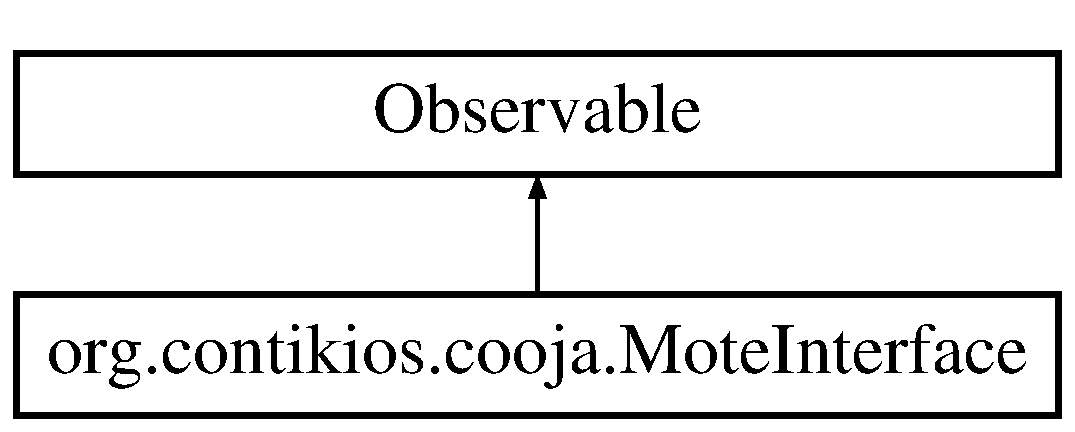
\includegraphics[height=2.000000cm]{classorg_1_1contikios_1_1cooja_1_1MoteInterface}
\end{center}
\end{figure}
\subsection*{Public Member Functions}
\begin{DoxyCompactItemize}
\item 
abstract J\-Panel \hyperlink{classorg_1_1contikios_1_1cooja_1_1MoteInterface_aec9b47d1b1a2f468eebb96b803608673}{get\-Interface\-Visualizer} ()
\item 
abstract void \hyperlink{classorg_1_1contikios_1_1cooja_1_1MoteInterface_a4f50d1a74a9cd0eac4ef28383869223e}{release\-Interface\-Visualizer} (J\-Panel panel)
\item 
abstract Collection$<$ Element $>$ \hyperlink{classorg_1_1contikios_1_1cooja_1_1MoteInterface_a36e4f41f720be08a8a04ec46a7184af1}{get\-Config\-X\-M\-L} ()
\item 
abstract void \hyperlink{classorg_1_1contikios_1_1cooja_1_1MoteInterface_a9b589b6bcc6687a0c4c1a473b4ef5723}{set\-Config\-X\-M\-L} (Collection$<$ Element $>$ config\-X\-M\-L, boolean vis\-Available)
\item 
void \hyperlink{classorg_1_1contikios_1_1cooja_1_1MoteInterface_af67ea5b5ccab50b236edf962bd4e600a}{removed} ()
\item 
void \hyperlink{classorg_1_1contikios_1_1cooja_1_1MoteInterface_afb51b7574cfc11ed6aa790ea9ff09344}{added} ()
\end{DoxyCompactItemize}
\subsection*{Static Public Member Functions}
\begin{DoxyCompactItemize}
\item 
static final \hyperlink{classorg_1_1contikios_1_1cooja_1_1MoteInterface}{Mote\-Interface} \hyperlink{classorg_1_1contikios_1_1cooja_1_1MoteInterface_af714a0ccfd23c543e3ed412dac6b317f}{generate\-Interface} (Class$<$?extends \hyperlink{classorg_1_1contikios_1_1cooja_1_1MoteInterface}{Mote\-Interface} $>$ interface\-Class, \hyperlink{interfaceorg_1_1contikios_1_1cooja_1_1Mote}{Mote} mote)
\end{DoxyCompactItemize}


\subsection{Detailed Description}
A mote interface represents a mote property. Typically, this is a simulated hardware peripheral such as a button or L\-E\-Ds. This may also be a property that the mote itself is unaware of, for example the current position of the mote.

Interfaces are the main way for the simulator to interact with a simulated mote.

Each interface can be polled before and after mote ticks. This is controlled by implementing the correct Java interfaces, such as Polled\-Before\-Active\-Ticks.

\begin{DoxySeeAlso}{See Also}
Polled\-Before\-Active\-Ticks 

Polled\-After\-Active\-Ticks 

Polled\-Before\-All\-Ticks 

Polled\-After\-All\-Ticks
\end{DoxySeeAlso}
\begin{DoxyAuthor}{Author}
Fredrik Osterlind 
\end{DoxyAuthor}


\subsection{Member Function Documentation}
\hypertarget{classorg_1_1contikios_1_1cooja_1_1MoteInterface_afb51b7574cfc11ed6aa790ea9ff09344}{\index{org\-::contikios\-::cooja\-::\-Mote\-Interface@{org\-::contikios\-::cooja\-::\-Mote\-Interface}!added@{added}}
\index{added@{added}!org::contikios::cooja::MoteInterface@{org\-::contikios\-::cooja\-::\-Mote\-Interface}}
\subsubsection[{added}]{\setlength{\rightskip}{0pt plus 5cm}void org.\-contikios.\-cooja.\-Mote\-Interface.\-added (
\begin{DoxyParamCaption}
{}
\end{DoxyParamCaption}
)\hspace{0.3cm}{\ttfamily [inline]}}}\label{classorg_1_1contikios_1_1cooja_1_1MoteInterface_afb51b7574cfc11ed6aa790ea9ff09344}
Called when all mote interfaces have been added to mote. \hypertarget{classorg_1_1contikios_1_1cooja_1_1MoteInterface_af714a0ccfd23c543e3ed412dac6b317f}{\index{org\-::contikios\-::cooja\-::\-Mote\-Interface@{org\-::contikios\-::cooja\-::\-Mote\-Interface}!generate\-Interface@{generate\-Interface}}
\index{generate\-Interface@{generate\-Interface}!org::contikios::cooja::MoteInterface@{org\-::contikios\-::cooja\-::\-Mote\-Interface}}
\subsubsection[{generate\-Interface}]{\setlength{\rightskip}{0pt plus 5cm}static final {\bf Mote\-Interface} org.\-contikios.\-cooja.\-Mote\-Interface.\-generate\-Interface (
\begin{DoxyParamCaption}
\item[{Class$<$?extends {\bf Mote\-Interface} $>$}]{interface\-Class, }
\item[{{\bf Mote}}]{mote}
\end{DoxyParamCaption}
)\hspace{0.3cm}{\ttfamily [inline]}, {\ttfamily [static]}}}\label{classorg_1_1contikios_1_1cooja_1_1MoteInterface_af714a0ccfd23c543e3ed412dac6b317f}
This method creates an instance of the given class with the given mote as constructor argument. Instead of calling the interface constructors directly this method may be used.


\begin{DoxyParams}{Parameters}
{\em interface\-Class} & \hyperlink{interfaceorg_1_1contikios_1_1cooja_1_1Mote}{Mote} interface class \\
\hline
{\em mote} & \hyperlink{interfaceorg_1_1contikios_1_1cooja_1_1Mote}{Mote} that will hold the interface \\
\hline
\end{DoxyParams}
\begin{DoxyReturn}{Returns}
\hyperlink{interfaceorg_1_1contikios_1_1cooja_1_1Mote}{Mote} interface instance 
\end{DoxyReturn}
\hypertarget{classorg_1_1contikios_1_1cooja_1_1MoteInterface_a36e4f41f720be08a8a04ec46a7184af1}{\index{org\-::contikios\-::cooja\-::\-Mote\-Interface@{org\-::contikios\-::cooja\-::\-Mote\-Interface}!get\-Config\-X\-M\-L@{get\-Config\-X\-M\-L}}
\index{get\-Config\-X\-M\-L@{get\-Config\-X\-M\-L}!org::contikios::cooja::MoteInterface@{org\-::contikios\-::cooja\-::\-Mote\-Interface}}
\subsubsection[{get\-Config\-X\-M\-L}]{\setlength{\rightskip}{0pt plus 5cm}abstract Collection$<$Element$>$ org.\-contikios.\-cooja.\-Mote\-Interface.\-get\-Config\-X\-M\-L (
\begin{DoxyParamCaption}
{}
\end{DoxyParamCaption}
)\hspace{0.3cm}{\ttfamily [abstract]}}}\label{classorg_1_1contikios_1_1cooja_1_1MoteInterface_a36e4f41f720be08a8a04ec46a7184af1}
Returns X\-M\-L elements representing the current config of this mote interface. This is fetched by the simulator for example when saving a simulation configuration file. For example an I\-P interface may return one element with the mote I\-P address. This method should however not return state specific information such as a log history. (All nodes are restarted when loading a simulation.)

\begin{DoxySeeAlso}{See Also}
\#set\-Config\-X\-M\-L(\-Collection, boolean) 
\end{DoxySeeAlso}
\begin{DoxyReturn}{Returns}
X\-M\-L elements representing the current interface config 
\end{DoxyReturn}
\hypertarget{classorg_1_1contikios_1_1cooja_1_1MoteInterface_aec9b47d1b1a2f468eebb96b803608673}{\index{org\-::contikios\-::cooja\-::\-Mote\-Interface@{org\-::contikios\-::cooja\-::\-Mote\-Interface}!get\-Interface\-Visualizer@{get\-Interface\-Visualizer}}
\index{get\-Interface\-Visualizer@{get\-Interface\-Visualizer}!org::contikios::cooja::MoteInterface@{org\-::contikios\-::cooja\-::\-Mote\-Interface}}
\subsubsection[{get\-Interface\-Visualizer}]{\setlength{\rightskip}{0pt plus 5cm}abstract J\-Panel org.\-contikios.\-cooja.\-Mote\-Interface.\-get\-Interface\-Visualizer (
\begin{DoxyParamCaption}
{}
\end{DoxyParamCaption}
)\hspace{0.3cm}{\ttfamily [abstract]}}}\label{classorg_1_1contikios_1_1cooja_1_1MoteInterface_aec9b47d1b1a2f468eebb96b803608673}
Returns a panel visualizing this interface. This could for example show last messages sent/received for a radio interface, or logged message for a log interface.

All panels returned from this method must later be released for memory reasons.

This method may return null.

\begin{DoxySeeAlso}{See Also}
\hyperlink{classorg_1_1contikios_1_1cooja_1_1MoteInterface_a4f50d1a74a9cd0eac4ef28383869223e}{release\-Interface\-Visualizer(\-J\-Panel)} 
\end{DoxySeeAlso}
\begin{DoxyReturn}{Returns}
Interface visualizer or null 
\end{DoxyReturn}
\hypertarget{classorg_1_1contikios_1_1cooja_1_1MoteInterface_a4f50d1a74a9cd0eac4ef28383869223e}{\index{org\-::contikios\-::cooja\-::\-Mote\-Interface@{org\-::contikios\-::cooja\-::\-Mote\-Interface}!release\-Interface\-Visualizer@{release\-Interface\-Visualizer}}
\index{release\-Interface\-Visualizer@{release\-Interface\-Visualizer}!org::contikios::cooja::MoteInterface@{org\-::contikios\-::cooja\-::\-Mote\-Interface}}
\subsubsection[{release\-Interface\-Visualizer}]{\setlength{\rightskip}{0pt plus 5cm}abstract void org.\-contikios.\-cooja.\-Mote\-Interface.\-release\-Interface\-Visualizer (
\begin{DoxyParamCaption}
\item[{J\-Panel}]{panel}
\end{DoxyParamCaption}
)\hspace{0.3cm}{\ttfamily [abstract]}}}\label{classorg_1_1contikios_1_1cooja_1_1MoteInterface_a4f50d1a74a9cd0eac4ef28383869223e}
This method should be called when a visualizer panel is no longer in use. Any resources of that panel, for example registered observers, will be released.

\begin{DoxySeeAlso}{See Also}
\hyperlink{classorg_1_1contikios_1_1cooja_1_1MoteInterface_aec9b47d1b1a2f468eebb96b803608673}{get\-Interface\-Visualizer()} 
\end{DoxySeeAlso}

\begin{DoxyParams}{Parameters}
{\em panel} & A interface visualizer panel fetched earlier for this mote interface. \\
\hline
\end{DoxyParams}
\hypertarget{classorg_1_1contikios_1_1cooja_1_1MoteInterface_af67ea5b5ccab50b236edf962bd4e600a}{\index{org\-::contikios\-::cooja\-::\-Mote\-Interface@{org\-::contikios\-::cooja\-::\-Mote\-Interface}!removed@{removed}}
\index{removed@{removed}!org::contikios::cooja::MoteInterface@{org\-::contikios\-::cooja\-::\-Mote\-Interface}}
\subsubsection[{removed}]{\setlength{\rightskip}{0pt plus 5cm}void org.\-contikios.\-cooja.\-Mote\-Interface.\-removed (
\begin{DoxyParamCaption}
{}
\end{DoxyParamCaption}
)\hspace{0.3cm}{\ttfamily [inline]}}}\label{classorg_1_1contikios_1_1cooja_1_1MoteInterface_af67ea5b5ccab50b236edf962bd4e600a}
Called to free resources used by the mote interface. This method is called when the mote is removed from the simulation. \hypertarget{classorg_1_1contikios_1_1cooja_1_1MoteInterface_a9b589b6bcc6687a0c4c1a473b4ef5723}{\index{org\-::contikios\-::cooja\-::\-Mote\-Interface@{org\-::contikios\-::cooja\-::\-Mote\-Interface}!set\-Config\-X\-M\-L@{set\-Config\-X\-M\-L}}
\index{set\-Config\-X\-M\-L@{set\-Config\-X\-M\-L}!org::contikios::cooja::MoteInterface@{org\-::contikios\-::cooja\-::\-Mote\-Interface}}
\subsubsection[{set\-Config\-X\-M\-L}]{\setlength{\rightskip}{0pt plus 5cm}abstract void org.\-contikios.\-cooja.\-Mote\-Interface.\-set\-Config\-X\-M\-L (
\begin{DoxyParamCaption}
\item[{Collection$<$ Element $>$}]{config\-X\-M\-L, }
\item[{boolean}]{vis\-Available}
\end{DoxyParamCaption}
)\hspace{0.3cm}{\ttfamily [abstract]}}}\label{classorg_1_1contikios_1_1cooja_1_1MoteInterface_a9b589b6bcc6687a0c4c1a473b4ef5723}
Sets the current mote interface config depending on the given X\-M\-L elements.

\begin{DoxySeeAlso}{See Also}
\hyperlink{classorg_1_1contikios_1_1cooja_1_1MoteInterface_a36e4f41f720be08a8a04ec46a7184af1}{get\-Config\-X\-M\-L()} 
\end{DoxySeeAlso}

\begin{DoxyParams}{Parameters}
{\em config\-X\-M\-L} & Config X\-M\-L elements \\
\hline
{\em vis\-Available} & Is this object allowed to show a visualizer? \\
\hline
\end{DoxyParams}


The documentation for this class was generated from the following file\-:\begin{DoxyCompactItemize}
\item 
Mote\-Interface.\-java\end{DoxyCompactItemize}

\hypertarget{classorg_1_1contikios_1_1cooja_1_1MoteInterfaceHandler}{\section{org.\-contikios.\-cooja.\-Mote\-Interface\-Handler Class Reference}
\label{classorg_1_1contikios_1_1cooja_1_1MoteInterfaceHandler}\index{org.\-contikios.\-cooja.\-Mote\-Interface\-Handler@{org.\-contikios.\-cooja.\-Mote\-Interface\-Handler}}
}
\subsection*{Public Member Functions}
\begin{DoxyCompactItemize}
\item 
\hyperlink{classorg_1_1contikios_1_1cooja_1_1MoteInterfaceHandler_a72f60f99130084750b9c51e4b09a3083}{Mote\-Interface\-Handler} ()
\item 
\hyperlink{classorg_1_1contikios_1_1cooja_1_1MoteInterfaceHandler_a2b5420f067a850e988da6d53d253b5e5}{Mote\-Interface\-Handler} (\hyperlink{interfaceorg_1_1contikios_1_1cooja_1_1Mote}{Mote} mote, Class$<$?extends \hyperlink{classorg_1_1contikios_1_1cooja_1_1MoteInterface}{Mote\-Interface} $>$\mbox{[}$\,$\mbox{]} interface\-Classes)
\item 
\hyperlink{classorg_1_1contikios_1_1cooja_1_1MoteInterface}{Mote\-Interface} \hyperlink{classorg_1_1contikios_1_1cooja_1_1MoteInterfaceHandler_a1bbbab6a19d416c59087bb78951628b3}{get} (String classname)
\item 
Battery \hyperlink{classorg_1_1contikios_1_1cooja_1_1MoteInterfaceHandler_ad1b97d695565157c9f9145bd585ab0f2}{get\-Battery} ()
\item 
Beeper \hyperlink{classorg_1_1contikios_1_1cooja_1_1MoteInterfaceHandler_a4331cc7577b2e09fd87e00ca6a1fc844}{get\-Beeper} ()
\item 
Button \hyperlink{classorg_1_1contikios_1_1cooja_1_1MoteInterfaceHandler_aa686e64d9f84f1b4906eea500c6798f4}{get\-Button} ()
\item 
Clock \hyperlink{classorg_1_1contikios_1_1cooja_1_1MoteInterfaceHandler_a668496b5a39f228fb2a17329677b2b13}{get\-Clock} ()
\item 
I\-P\-Address \hyperlink{classorg_1_1contikios_1_1cooja_1_1MoteInterfaceHandler_a9cfdbcabb9bd1b483c0c6b7ee39a64eb}{get\-I\-P\-Address} ()
\item 
Rime\-Address \hyperlink{classorg_1_1contikios_1_1cooja_1_1MoteInterfaceHandler_a8166f98272f183e940467c36de5b6a74}{get\-Rime\-Address} ()
\item 
L\-E\-D \hyperlink{classorg_1_1contikios_1_1cooja_1_1MoteInterfaceHandler_af9047c7f930b323a2bbd50beffe765f6}{get\-L\-E\-D} ()
\item 
Log \hyperlink{classorg_1_1contikios_1_1cooja_1_1MoteInterfaceHandler_a276edc9b54ed8549fd87b9f277118425}{get\-Log} ()
\item 
Mote\-I\-D \hyperlink{classorg_1_1contikios_1_1cooja_1_1MoteInterfaceHandler_a56e8ce372387424d3b76028e1bbc57c1}{get\-Mote\-I\-D} ()
\item 
P\-I\-R \hyperlink{classorg_1_1contikios_1_1cooja_1_1MoteInterfaceHandler_acde7bd2213e31bb044ebabe2dba27b16}{get\-P\-I\-R} ()
\item 
Position \hyperlink{classorg_1_1contikios_1_1cooja_1_1MoteInterfaceHandler_af6f171cc7e1fabb767f01ed70b8abaa9}{get\-Position} ()
\item 
Radio \hyperlink{classorg_1_1contikios_1_1cooja_1_1MoteInterfaceHandler_ab92cd221205b88b9f4ff34af051e5a8b}{get\-Radio} ()
\item 
void \hyperlink{classorg_1_1contikios_1_1cooja_1_1MoteInterfaceHandler_adb6e3304cc2a03769f61d3c51d84a439}{do\-Active\-Actions\-Before\-Tick} ()
\item 
void \hyperlink{classorg_1_1contikios_1_1cooja_1_1MoteInterfaceHandler_a40a6028e66b1d569b08290a0784aabe4}{do\-Active\-Actions\-After\-Tick} ()
\item 
void \hyperlink{classorg_1_1contikios_1_1cooja_1_1MoteInterfaceHandler_a13aaf685033814db9359c920e74261f0}{do\-Passive\-Actions\-Before\-Tick} ()
\item 
void \hyperlink{classorg_1_1contikios_1_1cooja_1_1MoteInterfaceHandler_a665063232706a8ca1fd7d9c1f00861b5}{do\-Passive\-Actions\-After\-Tick} ()
\item 
Collection$<$ \hyperlink{classorg_1_1contikios_1_1cooja_1_1MoteInterface}{Mote\-Interface} $>$ \hyperlink{classorg_1_1contikios_1_1cooja_1_1MoteInterfaceHandler_a1b3ea0eadba6762d997dfb6468c2e209}{get\-Interfaces} ()
\item 
void \hyperlink{classorg_1_1contikios_1_1cooja_1_1MoteInterfaceHandler_abca4b46a75c6d9f166bd12fa56a4a095}{add\-Interface} (\hyperlink{classorg_1_1contikios_1_1cooja_1_1MoteInterface}{Mote\-Interface} intf)
\item 
\hypertarget{classorg_1_1contikios_1_1cooja_1_1MoteInterfaceHandler_a710acc6a3d3077e61f9b3b3c467d49d2}{String {\bfseries to\-String} ()}\label{classorg_1_1contikios_1_1cooja_1_1MoteInterfaceHandler_a710acc6a3d3077e61f9b3b3c467d49d2}

\end{DoxyCompactItemize}


\subsection{Detailed Description}
The mote interface handler holds all interfaces for a specific mote. Interfaces should be polled via this class when the mote is ticked.

\begin{DoxySeeAlso}{See Also}
\hyperlink{classorg_1_1contikios_1_1cooja_1_1MoteInterfaceHandler_a40a6028e66b1d569b08290a0784aabe4}{do\-Active\-Actions\-After\-Tick()} 

\hyperlink{classorg_1_1contikios_1_1cooja_1_1MoteInterfaceHandler_adb6e3304cc2a03769f61d3c51d84a439}{do\-Active\-Actions\-Before\-Tick()} 

\hyperlink{classorg_1_1contikios_1_1cooja_1_1MoteInterfaceHandler_a665063232706a8ca1fd7d9c1f00861b5}{do\-Passive\-Actions\-After\-Tick()} 

\hyperlink{classorg_1_1contikios_1_1cooja_1_1MoteInterfaceHandler_a13aaf685033814db9359c920e74261f0}{do\-Passive\-Actions\-Before\-Tick()}
\end{DoxySeeAlso}
\begin{DoxyAuthor}{Author}
Fredrik Osterlind 
\end{DoxyAuthor}


\subsection{Constructor \& Destructor Documentation}
\hypertarget{classorg_1_1contikios_1_1cooja_1_1MoteInterfaceHandler_a72f60f99130084750b9c51e4b09a3083}{\index{org\-::contikios\-::cooja\-::\-Mote\-Interface\-Handler@{org\-::contikios\-::cooja\-::\-Mote\-Interface\-Handler}!Mote\-Interface\-Handler@{Mote\-Interface\-Handler}}
\index{Mote\-Interface\-Handler@{Mote\-Interface\-Handler}!org::contikios::cooja::MoteInterfaceHandler@{org\-::contikios\-::cooja\-::\-Mote\-Interface\-Handler}}
\subsubsection[{Mote\-Interface\-Handler}]{\setlength{\rightskip}{0pt plus 5cm}org.\-contikios.\-cooja.\-Mote\-Interface\-Handler.\-Mote\-Interface\-Handler (
\begin{DoxyParamCaption}
{}
\end{DoxyParamCaption}
)\hspace{0.3cm}{\ttfamily [inline]}}}\label{classorg_1_1contikios_1_1cooja_1_1MoteInterfaceHandler_a72f60f99130084750b9c51e4b09a3083}
Creates new empty mote interface handler. \hypertarget{classorg_1_1contikios_1_1cooja_1_1MoteInterfaceHandler_a2b5420f067a850e988da6d53d253b5e5}{\index{org\-::contikios\-::cooja\-::\-Mote\-Interface\-Handler@{org\-::contikios\-::cooja\-::\-Mote\-Interface\-Handler}!Mote\-Interface\-Handler@{Mote\-Interface\-Handler}}
\index{Mote\-Interface\-Handler@{Mote\-Interface\-Handler}!org::contikios::cooja::MoteInterfaceHandler@{org\-::contikios\-::cooja\-::\-Mote\-Interface\-Handler}}
\subsubsection[{Mote\-Interface\-Handler}]{\setlength{\rightskip}{0pt plus 5cm}org.\-contikios.\-cooja.\-Mote\-Interface\-Handler.\-Mote\-Interface\-Handler (
\begin{DoxyParamCaption}
\item[{{\bf Mote}}]{mote, }
\item[{Class$<$?extends {\bf Mote\-Interface} $>$\mbox{[}$\,$\mbox{]}}]{interface\-Classes}
\end{DoxyParamCaption}
)\hspace{0.3cm}{\ttfamily [inline]}}}\label{classorg_1_1contikios_1_1cooja_1_1MoteInterfaceHandler_a2b5420f067a850e988da6d53d253b5e5}
Creates new mote interface handler. All given interfaces are created.


\begin{DoxyParams}{Parameters}
{\em mote} & \hyperlink{interfaceorg_1_1contikios_1_1cooja_1_1Mote}{Mote} \\
\hline
{\em interface\-Classes} & \hyperlink{interfaceorg_1_1contikios_1_1cooja_1_1Mote}{Mote} interface classes \\
\hline
\end{DoxyParams}


\subsection{Member Function Documentation}
\hypertarget{classorg_1_1contikios_1_1cooja_1_1MoteInterfaceHandler_abca4b46a75c6d9f166bd12fa56a4a095}{\index{org\-::contikios\-::cooja\-::\-Mote\-Interface\-Handler@{org\-::contikios\-::cooja\-::\-Mote\-Interface\-Handler}!add\-Interface@{add\-Interface}}
\index{add\-Interface@{add\-Interface}!org::contikios::cooja::MoteInterfaceHandler@{org\-::contikios\-::cooja\-::\-Mote\-Interface\-Handler}}
\subsubsection[{add\-Interface}]{\setlength{\rightskip}{0pt plus 5cm}void org.\-contikios.\-cooja.\-Mote\-Interface\-Handler.\-add\-Interface (
\begin{DoxyParamCaption}
\item[{{\bf Mote\-Interface}}]{intf}
\end{DoxyParamCaption}
)\hspace{0.3cm}{\ttfamily [inline]}}}\label{classorg_1_1contikios_1_1cooja_1_1MoteInterfaceHandler_abca4b46a75c6d9f166bd12fa56a4a095}
Add mote interface.


\begin{DoxyParams}{Parameters}
{\em intf} & \hyperlink{interfaceorg_1_1contikios_1_1cooja_1_1Mote}{Mote} interface \\
\hline
\end{DoxyParams}
\begin{DoxySeeAlso}{See Also}
Polled\-Before\-Active\-Ticks 

Polled\-Before\-All\-Ticks 

Polled\-After\-Active\-Ticks 

Polled\-After\-All\-Ticks 
\end{DoxySeeAlso}
\hypertarget{classorg_1_1contikios_1_1cooja_1_1MoteInterfaceHandler_a40a6028e66b1d569b08290a0784aabe4}{\index{org\-::contikios\-::cooja\-::\-Mote\-Interface\-Handler@{org\-::contikios\-::cooja\-::\-Mote\-Interface\-Handler}!do\-Active\-Actions\-After\-Tick@{do\-Active\-Actions\-After\-Tick}}
\index{do\-Active\-Actions\-After\-Tick@{do\-Active\-Actions\-After\-Tick}!org::contikios::cooja::MoteInterfaceHandler@{org\-::contikios\-::cooja\-::\-Mote\-Interface\-Handler}}
\subsubsection[{do\-Active\-Actions\-After\-Tick}]{\setlength{\rightskip}{0pt plus 5cm}void org.\-contikios.\-cooja.\-Mote\-Interface\-Handler.\-do\-Active\-Actions\-After\-Tick (
\begin{DoxyParamCaption}
{}
\end{DoxyParamCaption}
)\hspace{0.3cm}{\ttfamily [inline]}}}\label{classorg_1_1contikios_1_1cooja_1_1MoteInterfaceHandler_a40a6028e66b1d569b08290a0784aabe4}
Polls active interfaces after mote tick. \hypertarget{classorg_1_1contikios_1_1cooja_1_1MoteInterfaceHandler_adb6e3304cc2a03769f61d3c51d84a439}{\index{org\-::contikios\-::cooja\-::\-Mote\-Interface\-Handler@{org\-::contikios\-::cooja\-::\-Mote\-Interface\-Handler}!do\-Active\-Actions\-Before\-Tick@{do\-Active\-Actions\-Before\-Tick}}
\index{do\-Active\-Actions\-Before\-Tick@{do\-Active\-Actions\-Before\-Tick}!org::contikios::cooja::MoteInterfaceHandler@{org\-::contikios\-::cooja\-::\-Mote\-Interface\-Handler}}
\subsubsection[{do\-Active\-Actions\-Before\-Tick}]{\setlength{\rightskip}{0pt plus 5cm}void org.\-contikios.\-cooja.\-Mote\-Interface\-Handler.\-do\-Active\-Actions\-Before\-Tick (
\begin{DoxyParamCaption}
{}
\end{DoxyParamCaption}
)\hspace{0.3cm}{\ttfamily [inline]}}}\label{classorg_1_1contikios_1_1cooja_1_1MoteInterfaceHandler_adb6e3304cc2a03769f61d3c51d84a439}
Polls active interfaces before mote tick. \hypertarget{classorg_1_1contikios_1_1cooja_1_1MoteInterfaceHandler_a665063232706a8ca1fd7d9c1f00861b5}{\index{org\-::contikios\-::cooja\-::\-Mote\-Interface\-Handler@{org\-::contikios\-::cooja\-::\-Mote\-Interface\-Handler}!do\-Passive\-Actions\-After\-Tick@{do\-Passive\-Actions\-After\-Tick}}
\index{do\-Passive\-Actions\-After\-Tick@{do\-Passive\-Actions\-After\-Tick}!org::contikios::cooja::MoteInterfaceHandler@{org\-::contikios\-::cooja\-::\-Mote\-Interface\-Handler}}
\subsubsection[{do\-Passive\-Actions\-After\-Tick}]{\setlength{\rightskip}{0pt plus 5cm}void org.\-contikios.\-cooja.\-Mote\-Interface\-Handler.\-do\-Passive\-Actions\-After\-Tick (
\begin{DoxyParamCaption}
{}
\end{DoxyParamCaption}
)\hspace{0.3cm}{\ttfamily [inline]}}}\label{classorg_1_1contikios_1_1cooja_1_1MoteInterfaceHandler_a665063232706a8ca1fd7d9c1f00861b5}
Polls passive interfaces after mote tick. \hypertarget{classorg_1_1contikios_1_1cooja_1_1MoteInterfaceHandler_a13aaf685033814db9359c920e74261f0}{\index{org\-::contikios\-::cooja\-::\-Mote\-Interface\-Handler@{org\-::contikios\-::cooja\-::\-Mote\-Interface\-Handler}!do\-Passive\-Actions\-Before\-Tick@{do\-Passive\-Actions\-Before\-Tick}}
\index{do\-Passive\-Actions\-Before\-Tick@{do\-Passive\-Actions\-Before\-Tick}!org::contikios::cooja::MoteInterfaceHandler@{org\-::contikios\-::cooja\-::\-Mote\-Interface\-Handler}}
\subsubsection[{do\-Passive\-Actions\-Before\-Tick}]{\setlength{\rightskip}{0pt plus 5cm}void org.\-contikios.\-cooja.\-Mote\-Interface\-Handler.\-do\-Passive\-Actions\-Before\-Tick (
\begin{DoxyParamCaption}
{}
\end{DoxyParamCaption}
)\hspace{0.3cm}{\ttfamily [inline]}}}\label{classorg_1_1contikios_1_1cooja_1_1MoteInterfaceHandler_a13aaf685033814db9359c920e74261f0}
Polls passive interfaces before mote tick. \hypertarget{classorg_1_1contikios_1_1cooja_1_1MoteInterfaceHandler_a1bbbab6a19d416c59087bb78951628b3}{\index{org\-::contikios\-::cooja\-::\-Mote\-Interface\-Handler@{org\-::contikios\-::cooja\-::\-Mote\-Interface\-Handler}!get@{get}}
\index{get@{get}!org::contikios::cooja::MoteInterfaceHandler@{org\-::contikios\-::cooja\-::\-Mote\-Interface\-Handler}}
\subsubsection[{get}]{\setlength{\rightskip}{0pt plus 5cm}{\bf Mote\-Interface} org.\-contikios.\-cooja.\-Mote\-Interface\-Handler.\-get (
\begin{DoxyParamCaption}
\item[{String}]{classname}
\end{DoxyParamCaption}
)\hspace{0.3cm}{\ttfamily [inline]}}}\label{classorg_1_1contikios_1_1cooja_1_1MoteInterfaceHandler_a1bbbab6a19d416c59087bb78951628b3}
Returns the first interface with a class name that ends with the given arguments. Example\-: mote.\-get\-Interfaces().get(\char`\"{}\-Temperature\char`\"{});


\begin{DoxyParams}{Parameters}
{\em $<$\-N$>$} & \\
\hline
{\em classname} & \\
\hline
\end{DoxyParams}
\begin{DoxyReturn}{Returns}

\end{DoxyReturn}
\hypertarget{classorg_1_1contikios_1_1cooja_1_1MoteInterfaceHandler_ad1b97d695565157c9f9145bd585ab0f2}{\index{org\-::contikios\-::cooja\-::\-Mote\-Interface\-Handler@{org\-::contikios\-::cooja\-::\-Mote\-Interface\-Handler}!get\-Battery@{get\-Battery}}
\index{get\-Battery@{get\-Battery}!org::contikios::cooja::MoteInterfaceHandler@{org\-::contikios\-::cooja\-::\-Mote\-Interface\-Handler}}
\subsubsection[{get\-Battery}]{\setlength{\rightskip}{0pt plus 5cm}Battery org.\-contikios.\-cooja.\-Mote\-Interface\-Handler.\-get\-Battery (
\begin{DoxyParamCaption}
{}
\end{DoxyParamCaption}
)\hspace{0.3cm}{\ttfamily [inline]}}}\label{classorg_1_1contikios_1_1cooja_1_1MoteInterfaceHandler_ad1b97d695565157c9f9145bd585ab0f2}
Returns the battery interface (if any).

\begin{DoxyReturn}{Returns}
Battery interface 
\end{DoxyReturn}
\hypertarget{classorg_1_1contikios_1_1cooja_1_1MoteInterfaceHandler_a4331cc7577b2e09fd87e00ca6a1fc844}{\index{org\-::contikios\-::cooja\-::\-Mote\-Interface\-Handler@{org\-::contikios\-::cooja\-::\-Mote\-Interface\-Handler}!get\-Beeper@{get\-Beeper}}
\index{get\-Beeper@{get\-Beeper}!org::contikios::cooja::MoteInterfaceHandler@{org\-::contikios\-::cooja\-::\-Mote\-Interface\-Handler}}
\subsubsection[{get\-Beeper}]{\setlength{\rightskip}{0pt plus 5cm}Beeper org.\-contikios.\-cooja.\-Mote\-Interface\-Handler.\-get\-Beeper (
\begin{DoxyParamCaption}
{}
\end{DoxyParamCaption}
)\hspace{0.3cm}{\ttfamily [inline]}}}\label{classorg_1_1contikios_1_1cooja_1_1MoteInterfaceHandler_a4331cc7577b2e09fd87e00ca6a1fc844}
Returns the beeper interface (if any).

\begin{DoxyReturn}{Returns}
Beeper interface 
\end{DoxyReturn}
\hypertarget{classorg_1_1contikios_1_1cooja_1_1MoteInterfaceHandler_aa686e64d9f84f1b4906eea500c6798f4}{\index{org\-::contikios\-::cooja\-::\-Mote\-Interface\-Handler@{org\-::contikios\-::cooja\-::\-Mote\-Interface\-Handler}!get\-Button@{get\-Button}}
\index{get\-Button@{get\-Button}!org::contikios::cooja::MoteInterfaceHandler@{org\-::contikios\-::cooja\-::\-Mote\-Interface\-Handler}}
\subsubsection[{get\-Button}]{\setlength{\rightskip}{0pt plus 5cm}Button org.\-contikios.\-cooja.\-Mote\-Interface\-Handler.\-get\-Button (
\begin{DoxyParamCaption}
{}
\end{DoxyParamCaption}
)\hspace{0.3cm}{\ttfamily [inline]}}}\label{classorg_1_1contikios_1_1cooja_1_1MoteInterfaceHandler_aa686e64d9f84f1b4906eea500c6798f4}
Returns the button interface (if any).

\begin{DoxyReturn}{Returns}
Button interface 
\end{DoxyReturn}
\hypertarget{classorg_1_1contikios_1_1cooja_1_1MoteInterfaceHandler_a668496b5a39f228fb2a17329677b2b13}{\index{org\-::contikios\-::cooja\-::\-Mote\-Interface\-Handler@{org\-::contikios\-::cooja\-::\-Mote\-Interface\-Handler}!get\-Clock@{get\-Clock}}
\index{get\-Clock@{get\-Clock}!org::contikios::cooja::MoteInterfaceHandler@{org\-::contikios\-::cooja\-::\-Mote\-Interface\-Handler}}
\subsubsection[{get\-Clock}]{\setlength{\rightskip}{0pt plus 5cm}Clock org.\-contikios.\-cooja.\-Mote\-Interface\-Handler.\-get\-Clock (
\begin{DoxyParamCaption}
{}
\end{DoxyParamCaption}
)\hspace{0.3cm}{\ttfamily [inline]}}}\label{classorg_1_1contikios_1_1cooja_1_1MoteInterfaceHandler_a668496b5a39f228fb2a17329677b2b13}
Returns the clock interface (if any).

\begin{DoxyReturn}{Returns}
Clock interface 
\end{DoxyReturn}
\hypertarget{classorg_1_1contikios_1_1cooja_1_1MoteInterfaceHandler_a1b3ea0eadba6762d997dfb6468c2e209}{\index{org\-::contikios\-::cooja\-::\-Mote\-Interface\-Handler@{org\-::contikios\-::cooja\-::\-Mote\-Interface\-Handler}!get\-Interfaces@{get\-Interfaces}}
\index{get\-Interfaces@{get\-Interfaces}!org::contikios::cooja::MoteInterfaceHandler@{org\-::contikios\-::cooja\-::\-Mote\-Interface\-Handler}}
\subsubsection[{get\-Interfaces}]{\setlength{\rightskip}{0pt plus 5cm}Collection$<${\bf Mote\-Interface}$>$ org.\-contikios.\-cooja.\-Mote\-Interface\-Handler.\-get\-Interfaces (
\begin{DoxyParamCaption}
{}
\end{DoxyParamCaption}
)\hspace{0.3cm}{\ttfamily [inline]}}}\label{classorg_1_1contikios_1_1cooja_1_1MoteInterfaceHandler_a1b3ea0eadba6762d997dfb6468c2e209}
\begin{DoxyReturn}{Returns}
\hyperlink{interfaceorg_1_1contikios_1_1cooja_1_1Mote}{Mote} interfaces 
\end{DoxyReturn}
\hypertarget{classorg_1_1contikios_1_1cooja_1_1MoteInterfaceHandler_a9cfdbcabb9bd1b483c0c6b7ee39a64eb}{\index{org\-::contikios\-::cooja\-::\-Mote\-Interface\-Handler@{org\-::contikios\-::cooja\-::\-Mote\-Interface\-Handler}!get\-I\-P\-Address@{get\-I\-P\-Address}}
\index{get\-I\-P\-Address@{get\-I\-P\-Address}!org::contikios::cooja::MoteInterfaceHandler@{org\-::contikios\-::cooja\-::\-Mote\-Interface\-Handler}}
\subsubsection[{get\-I\-P\-Address}]{\setlength{\rightskip}{0pt plus 5cm}I\-P\-Address org.\-contikios.\-cooja.\-Mote\-Interface\-Handler.\-get\-I\-P\-Address (
\begin{DoxyParamCaption}
{}
\end{DoxyParamCaption}
)\hspace{0.3cm}{\ttfamily [inline]}}}\label{classorg_1_1contikios_1_1cooja_1_1MoteInterfaceHandler_a9cfdbcabb9bd1b483c0c6b7ee39a64eb}
Returns the I\-P address interface (if any).

\begin{DoxyReturn}{Returns}
I\-P Address interface 
\end{DoxyReturn}
\hypertarget{classorg_1_1contikios_1_1cooja_1_1MoteInterfaceHandler_af9047c7f930b323a2bbd50beffe765f6}{\index{org\-::contikios\-::cooja\-::\-Mote\-Interface\-Handler@{org\-::contikios\-::cooja\-::\-Mote\-Interface\-Handler}!get\-L\-E\-D@{get\-L\-E\-D}}
\index{get\-L\-E\-D@{get\-L\-E\-D}!org::contikios::cooja::MoteInterfaceHandler@{org\-::contikios\-::cooja\-::\-Mote\-Interface\-Handler}}
\subsubsection[{get\-L\-E\-D}]{\setlength{\rightskip}{0pt plus 5cm}L\-E\-D org.\-contikios.\-cooja.\-Mote\-Interface\-Handler.\-get\-L\-E\-D (
\begin{DoxyParamCaption}
{}
\end{DoxyParamCaption}
)\hspace{0.3cm}{\ttfamily [inline]}}}\label{classorg_1_1contikios_1_1cooja_1_1MoteInterfaceHandler_af9047c7f930b323a2bbd50beffe765f6}
Returns the L\-E\-D interface (if any).

\begin{DoxyReturn}{Returns}
L\-E\-D interface 
\end{DoxyReturn}
\hypertarget{classorg_1_1contikios_1_1cooja_1_1MoteInterfaceHandler_a276edc9b54ed8549fd87b9f277118425}{\index{org\-::contikios\-::cooja\-::\-Mote\-Interface\-Handler@{org\-::contikios\-::cooja\-::\-Mote\-Interface\-Handler}!get\-Log@{get\-Log}}
\index{get\-Log@{get\-Log}!org::contikios::cooja::MoteInterfaceHandler@{org\-::contikios\-::cooja\-::\-Mote\-Interface\-Handler}}
\subsubsection[{get\-Log}]{\setlength{\rightskip}{0pt plus 5cm}Log org.\-contikios.\-cooja.\-Mote\-Interface\-Handler.\-get\-Log (
\begin{DoxyParamCaption}
{}
\end{DoxyParamCaption}
)\hspace{0.3cm}{\ttfamily [inline]}}}\label{classorg_1_1contikios_1_1cooja_1_1MoteInterfaceHandler_a276edc9b54ed8549fd87b9f277118425}
Returns the log interface (if any).

\begin{DoxyReturn}{Returns}
Log interface 
\end{DoxyReturn}
\hypertarget{classorg_1_1contikios_1_1cooja_1_1MoteInterfaceHandler_a56e8ce372387424d3b76028e1bbc57c1}{\index{org\-::contikios\-::cooja\-::\-Mote\-Interface\-Handler@{org\-::contikios\-::cooja\-::\-Mote\-Interface\-Handler}!get\-Mote\-I\-D@{get\-Mote\-I\-D}}
\index{get\-Mote\-I\-D@{get\-Mote\-I\-D}!org::contikios::cooja::MoteInterfaceHandler@{org\-::contikios\-::cooja\-::\-Mote\-Interface\-Handler}}
\subsubsection[{get\-Mote\-I\-D}]{\setlength{\rightskip}{0pt plus 5cm}Mote\-I\-D org.\-contikios.\-cooja.\-Mote\-Interface\-Handler.\-get\-Mote\-I\-D (
\begin{DoxyParamCaption}
{}
\end{DoxyParamCaption}
)\hspace{0.3cm}{\ttfamily [inline]}}}\label{classorg_1_1contikios_1_1cooja_1_1MoteInterfaceHandler_a56e8ce372387424d3b76028e1bbc57c1}
Returns the mote I\-D interface (if any).

\begin{DoxyReturn}{Returns}
\hyperlink{interfaceorg_1_1contikios_1_1cooja_1_1Mote}{Mote} I\-D interface 
\end{DoxyReturn}
\hypertarget{classorg_1_1contikios_1_1cooja_1_1MoteInterfaceHandler_acde7bd2213e31bb044ebabe2dba27b16}{\index{org\-::contikios\-::cooja\-::\-Mote\-Interface\-Handler@{org\-::contikios\-::cooja\-::\-Mote\-Interface\-Handler}!get\-P\-I\-R@{get\-P\-I\-R}}
\index{get\-P\-I\-R@{get\-P\-I\-R}!org::contikios::cooja::MoteInterfaceHandler@{org\-::contikios\-::cooja\-::\-Mote\-Interface\-Handler}}
\subsubsection[{get\-P\-I\-R}]{\setlength{\rightskip}{0pt plus 5cm}P\-I\-R org.\-contikios.\-cooja.\-Mote\-Interface\-Handler.\-get\-P\-I\-R (
\begin{DoxyParamCaption}
{}
\end{DoxyParamCaption}
)\hspace{0.3cm}{\ttfamily [inline]}}}\label{classorg_1_1contikios_1_1cooja_1_1MoteInterfaceHandler_acde7bd2213e31bb044ebabe2dba27b16}
Returns the P\-I\-R interface (if any).

\begin{DoxyReturn}{Returns}
P\-I\-R interface 
\end{DoxyReturn}
\hypertarget{classorg_1_1contikios_1_1cooja_1_1MoteInterfaceHandler_af6f171cc7e1fabb767f01ed70b8abaa9}{\index{org\-::contikios\-::cooja\-::\-Mote\-Interface\-Handler@{org\-::contikios\-::cooja\-::\-Mote\-Interface\-Handler}!get\-Position@{get\-Position}}
\index{get\-Position@{get\-Position}!org::contikios::cooja::MoteInterfaceHandler@{org\-::contikios\-::cooja\-::\-Mote\-Interface\-Handler}}
\subsubsection[{get\-Position}]{\setlength{\rightskip}{0pt plus 5cm}Position org.\-contikios.\-cooja.\-Mote\-Interface\-Handler.\-get\-Position (
\begin{DoxyParamCaption}
{}
\end{DoxyParamCaption}
)\hspace{0.3cm}{\ttfamily [inline]}}}\label{classorg_1_1contikios_1_1cooja_1_1MoteInterfaceHandler_af6f171cc7e1fabb767f01ed70b8abaa9}
Returns the position interface (if any).

\begin{DoxyReturn}{Returns}
Position interface 
\end{DoxyReturn}
\hypertarget{classorg_1_1contikios_1_1cooja_1_1MoteInterfaceHandler_ab92cd221205b88b9f4ff34af051e5a8b}{\index{org\-::contikios\-::cooja\-::\-Mote\-Interface\-Handler@{org\-::contikios\-::cooja\-::\-Mote\-Interface\-Handler}!get\-Radio@{get\-Radio}}
\index{get\-Radio@{get\-Radio}!org::contikios::cooja::MoteInterfaceHandler@{org\-::contikios\-::cooja\-::\-Mote\-Interface\-Handler}}
\subsubsection[{get\-Radio}]{\setlength{\rightskip}{0pt plus 5cm}Radio org.\-contikios.\-cooja.\-Mote\-Interface\-Handler.\-get\-Radio (
\begin{DoxyParamCaption}
{}
\end{DoxyParamCaption}
)\hspace{0.3cm}{\ttfamily [inline]}}}\label{classorg_1_1contikios_1_1cooja_1_1MoteInterfaceHandler_ab92cd221205b88b9f4ff34af051e5a8b}
Returns the radio interface (if any).

\begin{DoxyReturn}{Returns}
Radio interface 
\end{DoxyReturn}
\hypertarget{classorg_1_1contikios_1_1cooja_1_1MoteInterfaceHandler_a8166f98272f183e940467c36de5b6a74}{\index{org\-::contikios\-::cooja\-::\-Mote\-Interface\-Handler@{org\-::contikios\-::cooja\-::\-Mote\-Interface\-Handler}!get\-Rime\-Address@{get\-Rime\-Address}}
\index{get\-Rime\-Address@{get\-Rime\-Address}!org::contikios::cooja::MoteInterfaceHandler@{org\-::contikios\-::cooja\-::\-Mote\-Interface\-Handler}}
\subsubsection[{get\-Rime\-Address}]{\setlength{\rightskip}{0pt plus 5cm}Rime\-Address org.\-contikios.\-cooja.\-Mote\-Interface\-Handler.\-get\-Rime\-Address (
\begin{DoxyParamCaption}
{}
\end{DoxyParamCaption}
)\hspace{0.3cm}{\ttfamily [inline]}}}\label{classorg_1_1contikios_1_1cooja_1_1MoteInterfaceHandler_a8166f98272f183e940467c36de5b6a74}
\begin{DoxyReturn}{Returns}
Rime address interface 
\end{DoxyReturn}


The documentation for this class was generated from the following file\-:\begin{DoxyCompactItemize}
\item 
Mote\-Interface\-Handler.\-java\end{DoxyCompactItemize}

\hypertarget{interfaceorg_1_1contikios_1_1cooja_1_1MotePlugin}{\section{org.\-contikios.\-cooja.\-Mote\-Plugin Interface Reference}
\label{interfaceorg_1_1contikios_1_1cooja_1_1MotePlugin}\index{org.\-contikios.\-cooja.\-Mote\-Plugin@{org.\-contikios.\-cooja.\-Mote\-Plugin}}
}
\subsection*{Public Member Functions}
\begin{DoxyCompactItemize}
\item 
\hypertarget{interfaceorg_1_1contikios_1_1cooja_1_1MotePlugin_aded6cc666d06e6f8236356ba490d4147}{\hyperlink{interfaceorg_1_1contikios_1_1cooja_1_1Mote}{Mote} {\bfseries get\-Mote} ()}\label{interfaceorg_1_1contikios_1_1cooja_1_1MotePlugin_aded6cc666d06e6f8236356ba490d4147}

\end{DoxyCompactItemize}


The documentation for this interface was generated from the following file\-:\begin{DoxyCompactItemize}
\item 
Mote\-Plugin.\-java\end{DoxyCompactItemize}

\hypertarget{classorg_1_1contikios_1_1cooja_1_1MoteTimeEvent}{\section{org.\-contikios.\-cooja.\-Mote\-Time\-Event Class Reference}
\label{classorg_1_1contikios_1_1cooja_1_1MoteTimeEvent}\index{org.\-contikios.\-cooja.\-Mote\-Time\-Event@{org.\-contikios.\-cooja.\-Mote\-Time\-Event}}
}
Inheritance diagram for org.\-contikios.\-cooja.\-Mote\-Time\-Event\-:\begin{figure}[H]
\begin{center}
\leavevmode
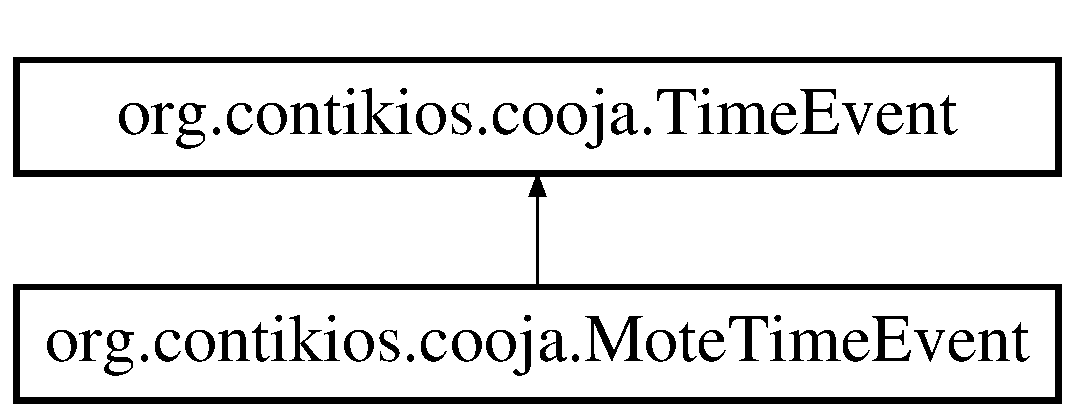
\includegraphics[height=2.000000cm]{classorg_1_1contikios_1_1cooja_1_1MoteTimeEvent}
\end{center}
\end{figure}
\subsection*{Public Member Functions}
\begin{DoxyCompactItemize}
\item 
\hypertarget{classorg_1_1contikios_1_1cooja_1_1MoteTimeEvent_a46be78ba957b24a731ef8b90839971dd}{{\bfseries Mote\-Time\-Event} (\hyperlink{interfaceorg_1_1contikios_1_1cooja_1_1Mote}{Mote} mote, long time)}\label{classorg_1_1contikios_1_1cooja_1_1MoteTimeEvent_a46be78ba957b24a731ef8b90839971dd}

\item 
\hypertarget{classorg_1_1contikios_1_1cooja_1_1MoteTimeEvent_af4a160f80571dcc7202fbbe9706e563e}{{\bfseries Mote\-Time\-Event} (\hyperlink{interfaceorg_1_1contikios_1_1cooja_1_1Mote}{Mote} mote, long time, String name)}\label{classorg_1_1contikios_1_1cooja_1_1MoteTimeEvent_af4a160f80571dcc7202fbbe9706e563e}

\item 
\hypertarget{classorg_1_1contikios_1_1cooja_1_1MoteTimeEvent_ad0b8edc53321833d1d430b5131c7d8c4}{\hyperlink{interfaceorg_1_1contikios_1_1cooja_1_1Mote}{Mote} {\bfseries get\-Mote} ()}\label{classorg_1_1contikios_1_1cooja_1_1MoteTimeEvent_ad0b8edc53321833d1d430b5131c7d8c4}

\end{DoxyCompactItemize}
\subsection*{Additional Inherited Members}


\subsection{Detailed Description}
Time event associated with a mote.

Used to automatically delete all time events of a specific mote, when the mote is removed from the simulation.

\begin{DoxySeeAlso}{See Also}
\hyperlink{classorg_1_1contikios_1_1cooja_1_1TimeEvent}{Time\-Event} 
\end{DoxySeeAlso}
\begin{DoxyAuthor}{Author}
Fredrik Osterlind 
\end{DoxyAuthor}


The documentation for this class was generated from the following file\-:\begin{DoxyCompactItemize}
\item 
Mote\-Time\-Event.\-java\end{DoxyCompactItemize}

\hypertarget{interfaceorg_1_1contikios_1_1cooja_1_1MoteType}{\section{org.\-contikios.\-cooja.\-Mote\-Type Interface Reference}
\label{interfaceorg_1_1contikios_1_1cooja_1_1MoteType}\index{org.\-contikios.\-cooja.\-Mote\-Type@{org.\-contikios.\-cooja.\-Mote\-Type}}
}
\subsection*{Classes}
\begin{DoxyCompactItemize}
\item 
class {\bfseries Mote\-Type\-Creation\-Exception}
\end{DoxyCompactItemize}
\subsection*{Public Member Functions}
\begin{DoxyCompactItemize}
\item 
String \hyperlink{interfaceorg_1_1contikios_1_1cooja_1_1MoteType_ad1882a7f2f3601919bb652528366fab0}{get\-Description} ()
\item 
void \hyperlink{interfaceorg_1_1contikios_1_1cooja_1_1MoteType_a92c342553b5fd0115dd0bb9d981f7817}{set\-Description} (String description)
\item 
String \hyperlink{interfaceorg_1_1contikios_1_1cooja_1_1MoteType_aa5c2986ffddcf15220a81cfcd6384957}{get\-Identifier} ()
\item 
void \hyperlink{interfaceorg_1_1contikios_1_1cooja_1_1MoteType_aee2769cce57b65416f5b0bda8da6c781}{set\-Identifier} (String identifier)
\item 
File \hyperlink{interfaceorg_1_1contikios_1_1cooja_1_1MoteType_a627bec8f129aa3d29dacc36adccc2f1d}{get\-Contiki\-Source\-File} ()
\item 
void \hyperlink{interfaceorg_1_1contikios_1_1cooja_1_1MoteType_a1336b4ddfdc6b7d0a3abad3ed5a0fbec}{set\-Contiki\-Source\-File} (File file)
\item 
File \hyperlink{interfaceorg_1_1contikios_1_1cooja_1_1MoteType_a7e89540390017160481dd301c767a910}{get\-Contiki\-Firmware\-File} ()
\item 
void \hyperlink{interfaceorg_1_1contikios_1_1cooja_1_1MoteType_a3ffbf1a84ca7faa90b1e397797006c15}{set\-Contiki\-Firmware\-File} (File file)
\item 
String \hyperlink{interfaceorg_1_1contikios_1_1cooja_1_1MoteType_ac47a5eea1447f155c3c44b940e30e0e3}{get\-Compile\-Commands} ()
\item 
void \hyperlink{interfaceorg_1_1contikios_1_1cooja_1_1MoteType_aca90f15a66d2563f8b85368f8e8141f5}{set\-Compile\-Commands} (String commands)
\item 
Class$<$?extends \hyperlink{classorg_1_1contikios_1_1cooja_1_1MoteInterface}{Mote\-Interface} $>$\mbox{[}$\,$\mbox{]} \hyperlink{interfaceorg_1_1contikios_1_1cooja_1_1MoteType_a2b78640d9f2bfcc67b9dd1947e7b267c}{get\-Mote\-Interface\-Classes} ()
\item 
void \hyperlink{interfaceorg_1_1contikios_1_1cooja_1_1MoteType_a56005afd3b0e73bccd098f51f209b411}{set\-Mote\-Interface\-Classes} (Class$<$?extends \hyperlink{classorg_1_1contikios_1_1cooja_1_1MoteInterface}{Mote\-Interface} $>$\mbox{[}$\,$\mbox{]} classes)
\item 
J\-Component \hyperlink{interfaceorg_1_1contikios_1_1cooja_1_1MoteType_aa61c6ade090027a69bf38d84f6194db4}{get\-Type\-Visualizer} ()
\item 
\hyperlink{classorg_1_1contikios_1_1cooja_1_1ProjectConfig}{Project\-Config} \hyperlink{interfaceorg_1_1contikios_1_1cooja_1_1MoteType_a96c0995e376950797ef6ae3da8b7c4ad}{get\-Config} ()
\item 
\hyperlink{interfaceorg_1_1contikios_1_1cooja_1_1Mote}{Mote} \hyperlink{interfaceorg_1_1contikios_1_1cooja_1_1MoteType_ae7196f6079178449410ed39f316c61bc}{generate\-Mote} (\hyperlink{classorg_1_1contikios_1_1cooja_1_1Simulation}{Simulation} simulation)
\item 
boolean \hyperlink{interfaceorg_1_1contikios_1_1cooja_1_1MoteType_a0f5fa8e60a5915b861e901de12bd3950}{configure\-And\-Init} (Container parent\-Container, \hyperlink{classorg_1_1contikios_1_1cooja_1_1Simulation}{Simulation} simulation, boolean vis\-Available)  throws Mote\-Type\-Creation\-Exception
\item 
Collection$<$ Element $>$ \hyperlink{interfaceorg_1_1contikios_1_1cooja_1_1MoteType_a657760f0f720ecd7c6e3c0f96d14eb4c}{get\-Config\-X\-M\-L} (\hyperlink{classorg_1_1contikios_1_1cooja_1_1Simulation}{Simulation} simulation)
\item 
boolean \hyperlink{interfaceorg_1_1contikios_1_1cooja_1_1MoteType_a3cfa85468d7f64ff7d2f28ee498cabca}{set\-Config\-X\-M\-L} (\hyperlink{classorg_1_1contikios_1_1cooja_1_1Simulation}{Simulation} simulation, Collection$<$ Element $>$ config\-X\-M\-L, boolean vis\-Available)  throws Mote\-Type\-Creation\-Exception
\end{DoxyCompactItemize}


\subsection{Detailed Description}
The mote type defines properties common for several motes. These properties may differ between different implementations, but typically includes how a mote is initialized, which hardware peripherals each mote has etc. All simulated motes belongs to one mote type.

A mote type may also hold the connection to an underlying simulation framework, such as a compiled Contiki system.

\begin{DoxySeeAlso}{See Also}
Contiki\-Mote\-Type 
\end{DoxySeeAlso}
\begin{DoxyAuthor}{Author}
Fredrik Osterlind 
\end{DoxyAuthor}


\subsection{Member Function Documentation}
\hypertarget{interfaceorg_1_1contikios_1_1cooja_1_1MoteType_a0f5fa8e60a5915b861e901de12bd3950}{\index{org\-::contikios\-::cooja\-::\-Mote\-Type@{org\-::contikios\-::cooja\-::\-Mote\-Type}!configure\-And\-Init@{configure\-And\-Init}}
\index{configure\-And\-Init@{configure\-And\-Init}!org::contikios::cooja::MoteType@{org\-::contikios\-::cooja\-::\-Mote\-Type}}
\subsubsection[{configure\-And\-Init}]{\setlength{\rightskip}{0pt plus 5cm}boolean org.\-contikios.\-cooja.\-Mote\-Type.\-configure\-And\-Init (
\begin{DoxyParamCaption}
\item[{Container}]{parent\-Container, }
\item[{{\bf Simulation}}]{simulation, }
\item[{boolean}]{vis\-Available}
\end{DoxyParamCaption}
) throws Mote\-Type\-Creation\-Exception}}\label{interfaceorg_1_1contikios_1_1cooja_1_1MoteType_a0f5fa8e60a5915b861e901de12bd3950}
This method configures and initializes a mote type ready to be used. It is called from the simulator when a new mote type is created. It may simply confirm that all settings are valid and return true, or display a dialog allowing a user to manually configure the mote type.

This method need normally only be run once per mote type!


\begin{DoxyParams}{Parameters}
{\em parent\-Container} & Parent container. May be null if not visualized. \\
\hline
{\em simulation} & \hyperlink{classorg_1_1contikios_1_1cooja_1_1Simulation}{Simulation} holding (or that should hold) mote type \\
\hline
{\em vis\-Available} & True if this method is allowed to show a visualizer \\
\hline
\end{DoxyParams}
\begin{DoxyReturn}{Returns}
True if mote type has valid settings and is ready to be used 
\end{DoxyReturn}
\hypertarget{interfaceorg_1_1contikios_1_1cooja_1_1MoteType_ae7196f6079178449410ed39f316c61bc}{\index{org\-::contikios\-::cooja\-::\-Mote\-Type@{org\-::contikios\-::cooja\-::\-Mote\-Type}!generate\-Mote@{generate\-Mote}}
\index{generate\-Mote@{generate\-Mote}!org::contikios::cooja::MoteType@{org\-::contikios\-::cooja\-::\-Mote\-Type}}
\subsubsection[{generate\-Mote}]{\setlength{\rightskip}{0pt plus 5cm}{\bf Mote} org.\-contikios.\-cooja.\-Mote\-Type.\-generate\-Mote (
\begin{DoxyParamCaption}
\item[{{\bf Simulation}}]{simulation}
\end{DoxyParamCaption}
)}}\label{interfaceorg_1_1contikios_1_1cooja_1_1MoteType_ae7196f6079178449410ed39f316c61bc}
Generates a mote of this mote type.


\begin{DoxyParams}{Parameters}
{\em simulation} & \hyperlink{classorg_1_1contikios_1_1cooja_1_1Simulation}{Simulation} that will contain mote \\
\hline
\end{DoxyParams}
\begin{DoxyReturn}{Returns}
New mote 
\end{DoxyReturn}
\hypertarget{interfaceorg_1_1contikios_1_1cooja_1_1MoteType_ac47a5eea1447f155c3c44b940e30e0e3}{\index{org\-::contikios\-::cooja\-::\-Mote\-Type@{org\-::contikios\-::cooja\-::\-Mote\-Type}!get\-Compile\-Commands@{get\-Compile\-Commands}}
\index{get\-Compile\-Commands@{get\-Compile\-Commands}!org::contikios::cooja::MoteType@{org\-::contikios\-::cooja\-::\-Mote\-Type}}
\subsubsection[{get\-Compile\-Commands}]{\setlength{\rightskip}{0pt plus 5cm}String org.\-contikios.\-cooja.\-Mote\-Type.\-get\-Compile\-Commands (
\begin{DoxyParamCaption}
{}
\end{DoxyParamCaption}
)}}\label{interfaceorg_1_1contikios_1_1cooja_1_1MoteType_ac47a5eea1447f155c3c44b940e30e0e3}
Commands used to build the Contiki firmware from the Contiki source. May be null.

\begin{DoxyReturn}{Returns}
Compile commands used to build firmware 
\end{DoxyReturn}
\begin{DoxySeeAlso}{See Also}
\hyperlink{interfaceorg_1_1contikios_1_1cooja_1_1MoteType_aca90f15a66d2563f8b85368f8e8141f5}{set\-Compile\-Commands(\-String)} 

\hyperlink{interfaceorg_1_1contikios_1_1cooja_1_1MoteType_a7e89540390017160481dd301c767a910}{get\-Contiki\-Firmware\-File()} 

\hyperlink{interfaceorg_1_1contikios_1_1cooja_1_1MoteType_a627bec8f129aa3d29dacc36adccc2f1d}{get\-Contiki\-Source\-File()} 
\end{DoxySeeAlso}
\hypertarget{interfaceorg_1_1contikios_1_1cooja_1_1MoteType_a96c0995e376950797ef6ae3da8b7c4ad}{\index{org\-::contikios\-::cooja\-::\-Mote\-Type@{org\-::contikios\-::cooja\-::\-Mote\-Type}!get\-Config@{get\-Config}}
\index{get\-Config@{get\-Config}!org::contikios::cooja::MoteType@{org\-::contikios\-::cooja\-::\-Mote\-Type}}
\subsubsection[{get\-Config}]{\setlength{\rightskip}{0pt plus 5cm}{\bf Project\-Config} org.\-contikios.\-cooja.\-Mote\-Type.\-get\-Config (
\begin{DoxyParamCaption}
{}
\end{DoxyParamCaption}
)}}\label{interfaceorg_1_1contikios_1_1cooja_1_1MoteType_a96c0995e376950797ef6ae3da8b7c4ad}
Returns this mote type's project configuration.

\begin{DoxyReturn}{Returns}
Project configuration 
\end{DoxyReturn}
\hypertarget{interfaceorg_1_1contikios_1_1cooja_1_1MoteType_a657760f0f720ecd7c6e3c0f96d14eb4c}{\index{org\-::contikios\-::cooja\-::\-Mote\-Type@{org\-::contikios\-::cooja\-::\-Mote\-Type}!get\-Config\-X\-M\-L@{get\-Config\-X\-M\-L}}
\index{get\-Config\-X\-M\-L@{get\-Config\-X\-M\-L}!org::contikios::cooja::MoteType@{org\-::contikios\-::cooja\-::\-Mote\-Type}}
\subsubsection[{get\-Config\-X\-M\-L}]{\setlength{\rightskip}{0pt plus 5cm}Collection$<$Element$>$ org.\-contikios.\-cooja.\-Mote\-Type.\-get\-Config\-X\-M\-L (
\begin{DoxyParamCaption}
\item[{{\bf Simulation}}]{simulation}
\end{DoxyParamCaption}
)}}\label{interfaceorg_1_1contikios_1_1cooja_1_1MoteType_a657760f0f720ecd7c6e3c0f96d14eb4c}
Returns X\-M\-L elements representing the current config of this mote type. This is fetched by the simulator for example when saving a simulation configuration file. For example a Contiki base directory may be saved.

\begin{DoxySeeAlso}{See Also}
\#set\-Config\-X\-M\-L(\-Simulation, Collection, boolean) 
\end{DoxySeeAlso}

\begin{DoxyParams}{Parameters}
{\em simulation} & Current simulation \\
\hline
\end{DoxyParams}
\begin{DoxyReturn}{Returns}
X\-M\-L elements representing the current mote type's config 
\end{DoxyReturn}
\hypertarget{interfaceorg_1_1contikios_1_1cooja_1_1MoteType_a7e89540390017160481dd301c767a910}{\index{org\-::contikios\-::cooja\-::\-Mote\-Type@{org\-::contikios\-::cooja\-::\-Mote\-Type}!get\-Contiki\-Firmware\-File@{get\-Contiki\-Firmware\-File}}
\index{get\-Contiki\-Firmware\-File@{get\-Contiki\-Firmware\-File}!org::contikios::cooja::MoteType@{org\-::contikios\-::cooja\-::\-Mote\-Type}}
\subsubsection[{get\-Contiki\-Firmware\-File}]{\setlength{\rightskip}{0pt plus 5cm}File org.\-contikios.\-cooja.\-Mote\-Type.\-get\-Contiki\-Firmware\-File (
\begin{DoxyParamCaption}
{}
\end{DoxyParamCaption}
)}}\label{interfaceorg_1_1contikios_1_1cooja_1_1MoteType_a7e89540390017160481dd301c767a910}
Compiled Contiki firmware file or library. May be null.

\begin{DoxyReturn}{Returns}
Contiki firmware file or library. 
\end{DoxyReturn}
\begin{DoxySeeAlso}{See Also}
\hyperlink{interfaceorg_1_1contikios_1_1cooja_1_1MoteType_a3ffbf1a84ca7faa90b1e397797006c15}{set\-Contiki\-Firmware\-File(\-File)} 
\end{DoxySeeAlso}
\hypertarget{interfaceorg_1_1contikios_1_1cooja_1_1MoteType_a627bec8f129aa3d29dacc36adccc2f1d}{\index{org\-::contikios\-::cooja\-::\-Mote\-Type@{org\-::contikios\-::cooja\-::\-Mote\-Type}!get\-Contiki\-Source\-File@{get\-Contiki\-Source\-File}}
\index{get\-Contiki\-Source\-File@{get\-Contiki\-Source\-File}!org::contikios::cooja::MoteType@{org\-::contikios\-::cooja\-::\-Mote\-Type}}
\subsubsection[{get\-Contiki\-Source\-File}]{\setlength{\rightskip}{0pt plus 5cm}File org.\-contikios.\-cooja.\-Mote\-Type.\-get\-Contiki\-Source\-File (
\begin{DoxyParamCaption}
{}
\end{DoxyParamCaption}
)}}\label{interfaceorg_1_1contikios_1_1cooja_1_1MoteType_a627bec8f129aa3d29dacc36adccc2f1d}
Main Contiki source file of mote type. May be null.

\begin{DoxyReturn}{Returns}
Contiki main process source file. 
\end{DoxyReturn}
\begin{DoxySeeAlso}{See Also}
\hyperlink{interfaceorg_1_1contikios_1_1cooja_1_1MoteType_a1336b4ddfdc6b7d0a3abad3ed5a0fbec}{set\-Contiki\-Source\-File(\-File)} 
\end{DoxySeeAlso}
\hypertarget{interfaceorg_1_1contikios_1_1cooja_1_1MoteType_ad1882a7f2f3601919bb652528366fab0}{\index{org\-::contikios\-::cooja\-::\-Mote\-Type@{org\-::contikios\-::cooja\-::\-Mote\-Type}!get\-Description@{get\-Description}}
\index{get\-Description@{get\-Description}!org::contikios::cooja::MoteType@{org\-::contikios\-::cooja\-::\-Mote\-Type}}
\subsubsection[{get\-Description}]{\setlength{\rightskip}{0pt plus 5cm}String org.\-contikios.\-cooja.\-Mote\-Type.\-get\-Description (
\begin{DoxyParamCaption}
{}
\end{DoxyParamCaption}
)}}\label{interfaceorg_1_1contikios_1_1cooja_1_1MoteType_ad1882a7f2f3601919bb652528366fab0}
Returns the mote type description.

\begin{DoxyReturn}{Returns}
Description 
\end{DoxyReturn}
\hypertarget{interfaceorg_1_1contikios_1_1cooja_1_1MoteType_aa5c2986ffddcf15220a81cfcd6384957}{\index{org\-::contikios\-::cooja\-::\-Mote\-Type@{org\-::contikios\-::cooja\-::\-Mote\-Type}!get\-Identifier@{get\-Identifier}}
\index{get\-Identifier@{get\-Identifier}!org::contikios::cooja::MoteType@{org\-::contikios\-::cooja\-::\-Mote\-Type}}
\subsubsection[{get\-Identifier}]{\setlength{\rightskip}{0pt plus 5cm}String org.\-contikios.\-cooja.\-Mote\-Type.\-get\-Identifier (
\begin{DoxyParamCaption}
{}
\end{DoxyParamCaption}
)}}\label{interfaceorg_1_1contikios_1_1cooja_1_1MoteType_aa5c2986ffddcf15220a81cfcd6384957}
Returns the mote type identifier.

\begin{DoxyReturn}{Returns}
\hyperlink{interfaceorg_1_1contikios_1_1cooja_1_1Mote}{Mote} type identifier 
\end{DoxyReturn}
\hypertarget{interfaceorg_1_1contikios_1_1cooja_1_1MoteType_a2b78640d9f2bfcc67b9dd1947e7b267c}{\index{org\-::contikios\-::cooja\-::\-Mote\-Type@{org\-::contikios\-::cooja\-::\-Mote\-Type}!get\-Mote\-Interface\-Classes@{get\-Mote\-Interface\-Classes}}
\index{get\-Mote\-Interface\-Classes@{get\-Mote\-Interface\-Classes}!org::contikios::cooja::MoteType@{org\-::contikios\-::cooja\-::\-Mote\-Type}}
\subsubsection[{get\-Mote\-Interface\-Classes}]{\setlength{\rightskip}{0pt plus 5cm}Class$<$? extends {\bf Mote\-Interface}$>$ \mbox{[}$\,$\mbox{]} org.\-contikios.\-cooja.\-Mote\-Type.\-get\-Mote\-Interface\-Classes (
\begin{DoxyParamCaption}
{}
\end{DoxyParamCaption}
)}}\label{interfaceorg_1_1contikios_1_1cooja_1_1MoteType_a2b78640d9f2bfcc67b9dd1947e7b267c}
\begin{DoxyReturn}{Returns}
\hyperlink{interfaceorg_1_1contikios_1_1cooja_1_1Mote}{Mote} interface classes of mote type. 
\end{DoxyReturn}
\begin{DoxySeeAlso}{See Also}
\#set\-Mote\-Interface\-Classes(\-Class\mbox{[}$\,$\mbox{]}) 
\end{DoxySeeAlso}
\hypertarget{interfaceorg_1_1contikios_1_1cooja_1_1MoteType_aa61c6ade090027a69bf38d84f6194db4}{\index{org\-::contikios\-::cooja\-::\-Mote\-Type@{org\-::contikios\-::cooja\-::\-Mote\-Type}!get\-Type\-Visualizer@{get\-Type\-Visualizer}}
\index{get\-Type\-Visualizer@{get\-Type\-Visualizer}!org::contikios::cooja::MoteType@{org\-::contikios\-::cooja\-::\-Mote\-Type}}
\subsubsection[{get\-Type\-Visualizer}]{\setlength{\rightskip}{0pt plus 5cm}J\-Component org.\-contikios.\-cooja.\-Mote\-Type.\-get\-Type\-Visualizer (
\begin{DoxyParamCaption}
{}
\end{DoxyParamCaption}
)}}\label{interfaceorg_1_1contikios_1_1cooja_1_1MoteType_aa61c6ade090027a69bf38d84f6194db4}
Returns a panel with mote type specific data. May be null.

\begin{DoxyReturn}{Returns}
\hyperlink{interfaceorg_1_1contikios_1_1cooja_1_1Mote}{Mote} type visualizer 
\end{DoxyReturn}
\hypertarget{interfaceorg_1_1contikios_1_1cooja_1_1MoteType_aca90f15a66d2563f8b85368f8e8141f5}{\index{org\-::contikios\-::cooja\-::\-Mote\-Type@{org\-::contikios\-::cooja\-::\-Mote\-Type}!set\-Compile\-Commands@{set\-Compile\-Commands}}
\index{set\-Compile\-Commands@{set\-Compile\-Commands}!org::contikios::cooja::MoteType@{org\-::contikios\-::cooja\-::\-Mote\-Type}}
\subsubsection[{set\-Compile\-Commands}]{\setlength{\rightskip}{0pt plus 5cm}void org.\-contikios.\-cooja.\-Mote\-Type.\-set\-Compile\-Commands (
\begin{DoxyParamCaption}
\item[{String}]{commands}
\end{DoxyParamCaption}
)}}\label{interfaceorg_1_1contikios_1_1cooja_1_1MoteType_aca90f15a66d2563f8b85368f8e8141f5}

\begin{DoxyParams}{Parameters}
{\em commands} & Compile commands \\
\hline
\end{DoxyParams}
\begin{DoxySeeAlso}{See Also}
\hyperlink{interfaceorg_1_1contikios_1_1cooja_1_1MoteType_ac47a5eea1447f155c3c44b940e30e0e3}{get\-Compile\-Commands()} 
\end{DoxySeeAlso}
\hypertarget{interfaceorg_1_1contikios_1_1cooja_1_1MoteType_a3cfa85468d7f64ff7d2f28ee498cabca}{\index{org\-::contikios\-::cooja\-::\-Mote\-Type@{org\-::contikios\-::cooja\-::\-Mote\-Type}!set\-Config\-X\-M\-L@{set\-Config\-X\-M\-L}}
\index{set\-Config\-X\-M\-L@{set\-Config\-X\-M\-L}!org::contikios::cooja::MoteType@{org\-::contikios\-::cooja\-::\-Mote\-Type}}
\subsubsection[{set\-Config\-X\-M\-L}]{\setlength{\rightskip}{0pt plus 5cm}boolean org.\-contikios.\-cooja.\-Mote\-Type.\-set\-Config\-X\-M\-L (
\begin{DoxyParamCaption}
\item[{{\bf Simulation}}]{simulation, }
\item[{Collection$<$ Element $>$}]{config\-X\-M\-L, }
\item[{boolean}]{vis\-Available}
\end{DoxyParamCaption}
) throws Mote\-Type\-Creation\-Exception}}\label{interfaceorg_1_1contikios_1_1cooja_1_1MoteType_a3cfa85468d7f64ff7d2f28ee498cabca}
Sets the current mote type config depending on the given X\-M\-L elements. Observe that this method is responsible for restoring the configuration depending on the given arguments. This may include recompiling and loading libraries.

\begin{DoxySeeAlso}{See Also}
\hyperlink{interfaceorg_1_1contikios_1_1cooja_1_1MoteType_a657760f0f720ecd7c6e3c0f96d14eb4c}{get\-Config\-X\-M\-L()} 
\end{DoxySeeAlso}

\begin{DoxyParams}{Parameters}
{\em simulation} & \hyperlink{classorg_1_1contikios_1_1cooja_1_1Simulation}{Simulation} that will hold the mote type \\
\hline
{\em config\-X\-M\-L} & Config X\-M\-L elements \\
\hline
{\em vis\-Available} & True if this method is allowed to show a visualizer \\
\hline
\end{DoxyParams}
\begin{DoxyReturn}{Returns}
True if config was set successfully, false otherwise 
\end{DoxyReturn}
\hypertarget{interfaceorg_1_1contikios_1_1cooja_1_1MoteType_a3ffbf1a84ca7faa90b1e397797006c15}{\index{org\-::contikios\-::cooja\-::\-Mote\-Type@{org\-::contikios\-::cooja\-::\-Mote\-Type}!set\-Contiki\-Firmware\-File@{set\-Contiki\-Firmware\-File}}
\index{set\-Contiki\-Firmware\-File@{set\-Contiki\-Firmware\-File}!org::contikios::cooja::MoteType@{org\-::contikios\-::cooja\-::\-Mote\-Type}}
\subsubsection[{set\-Contiki\-Firmware\-File}]{\setlength{\rightskip}{0pt plus 5cm}void org.\-contikios.\-cooja.\-Mote\-Type.\-set\-Contiki\-Firmware\-File (
\begin{DoxyParamCaption}
\item[{File}]{file}
\end{DoxyParamCaption}
)}}\label{interfaceorg_1_1contikios_1_1cooja_1_1MoteType_a3ffbf1a84ca7faa90b1e397797006c15}

\begin{DoxyParams}{Parameters}
{\em file} & Contiki firmware file or library. \\
\hline
\end{DoxyParams}
\begin{DoxySeeAlso}{See Also}
\hyperlink{interfaceorg_1_1contikios_1_1cooja_1_1MoteType_a7e89540390017160481dd301c767a910}{get\-Contiki\-Firmware\-File()} 
\end{DoxySeeAlso}
\hypertarget{interfaceorg_1_1contikios_1_1cooja_1_1MoteType_a1336b4ddfdc6b7d0a3abad3ed5a0fbec}{\index{org\-::contikios\-::cooja\-::\-Mote\-Type@{org\-::contikios\-::cooja\-::\-Mote\-Type}!set\-Contiki\-Source\-File@{set\-Contiki\-Source\-File}}
\index{set\-Contiki\-Source\-File@{set\-Contiki\-Source\-File}!org::contikios::cooja::MoteType@{org\-::contikios\-::cooja\-::\-Mote\-Type}}
\subsubsection[{set\-Contiki\-Source\-File}]{\setlength{\rightskip}{0pt plus 5cm}void org.\-contikios.\-cooja.\-Mote\-Type.\-set\-Contiki\-Source\-File (
\begin{DoxyParamCaption}
\item[{File}]{file}
\end{DoxyParamCaption}
)}}\label{interfaceorg_1_1contikios_1_1cooja_1_1MoteType_a1336b4ddfdc6b7d0a3abad3ed5a0fbec}

\begin{DoxyParams}{Parameters}
{\em file} & Contiki main process source file. \\
\hline
\end{DoxyParams}
\begin{DoxySeeAlso}{See Also}
\hyperlink{interfaceorg_1_1contikios_1_1cooja_1_1MoteType_a627bec8f129aa3d29dacc36adccc2f1d}{get\-Contiki\-Source\-File()} 
\end{DoxySeeAlso}
\hypertarget{interfaceorg_1_1contikios_1_1cooja_1_1MoteType_a92c342553b5fd0115dd0bb9d981f7817}{\index{org\-::contikios\-::cooja\-::\-Mote\-Type@{org\-::contikios\-::cooja\-::\-Mote\-Type}!set\-Description@{set\-Description}}
\index{set\-Description@{set\-Description}!org::contikios::cooja::MoteType@{org\-::contikios\-::cooja\-::\-Mote\-Type}}
\subsubsection[{set\-Description}]{\setlength{\rightskip}{0pt plus 5cm}void org.\-contikios.\-cooja.\-Mote\-Type.\-set\-Description (
\begin{DoxyParamCaption}
\item[{String}]{description}
\end{DoxyParamCaption}
)}}\label{interfaceorg_1_1contikios_1_1cooja_1_1MoteType_a92c342553b5fd0115dd0bb9d981f7817}
Sets the mote type description.


\begin{DoxyParams}{Parameters}
{\em description} & New description \\
\hline
\end{DoxyParams}
\hypertarget{interfaceorg_1_1contikios_1_1cooja_1_1MoteType_aee2769cce57b65416f5b0bda8da6c781}{\index{org\-::contikios\-::cooja\-::\-Mote\-Type@{org\-::contikios\-::cooja\-::\-Mote\-Type}!set\-Identifier@{set\-Identifier}}
\index{set\-Identifier@{set\-Identifier}!org::contikios::cooja::MoteType@{org\-::contikios\-::cooja\-::\-Mote\-Type}}
\subsubsection[{set\-Identifier}]{\setlength{\rightskip}{0pt plus 5cm}void org.\-contikios.\-cooja.\-Mote\-Type.\-set\-Identifier (
\begin{DoxyParamCaption}
\item[{String}]{identifier}
\end{DoxyParamCaption}
)}}\label{interfaceorg_1_1contikios_1_1cooja_1_1MoteType_aee2769cce57b65416f5b0bda8da6c781}
Sets the mote type identifier.


\begin{DoxyParams}{Parameters}
{\em identifier} & New identifier \\
\hline
\end{DoxyParams}
\hypertarget{interfaceorg_1_1contikios_1_1cooja_1_1MoteType_a56005afd3b0e73bccd098f51f209b411}{\index{org\-::contikios\-::cooja\-::\-Mote\-Type@{org\-::contikios\-::cooja\-::\-Mote\-Type}!set\-Mote\-Interface\-Classes@{set\-Mote\-Interface\-Classes}}
\index{set\-Mote\-Interface\-Classes@{set\-Mote\-Interface\-Classes}!org::contikios::cooja::MoteType@{org\-::contikios\-::cooja\-::\-Mote\-Type}}
\subsubsection[{set\-Mote\-Interface\-Classes}]{\setlength{\rightskip}{0pt plus 5cm}void org.\-contikios.\-cooja.\-Mote\-Type.\-set\-Mote\-Interface\-Classes (
\begin{DoxyParamCaption}
\item[{Class$<$?extends {\bf Mote\-Interface} $>$\mbox{[}$\,$\mbox{]}}]{classes}
\end{DoxyParamCaption}
)}}\label{interfaceorg_1_1contikios_1_1cooja_1_1MoteType_a56005afd3b0e73bccd098f51f209b411}
Sets mote interface Java classes of mote type.


\begin{DoxyParams}{Parameters}
{\em classes} & \hyperlink{interfaceorg_1_1contikios_1_1cooja_1_1Mote}{Mote} interface classes \\
\hline
\end{DoxyParams}


The documentation for this interface was generated from the following file\-:\begin{DoxyCompactItemize}
\item 
Mote\-Type.\-java\end{DoxyCompactItemize}

\hypertarget{classorg_1_1contikios_1_1cooja_1_1Cooja_1_1ParseProjectsException}{\section{org.\-contikios.\-cooja.\-Cooja.\-Parse\-Projects\-Exception Class Reference}
\label{classorg_1_1contikios_1_1cooja_1_1Cooja_1_1ParseProjectsException}\index{org.\-contikios.\-cooja.\-Cooja.\-Parse\-Projects\-Exception@{org.\-contikios.\-cooja.\-Cooja.\-Parse\-Projects\-Exception}}
}
Inheritance diagram for org.\-contikios.\-cooja.\-Cooja.\-Parse\-Projects\-Exception\-:\begin{figure}[H]
\begin{center}
\leavevmode
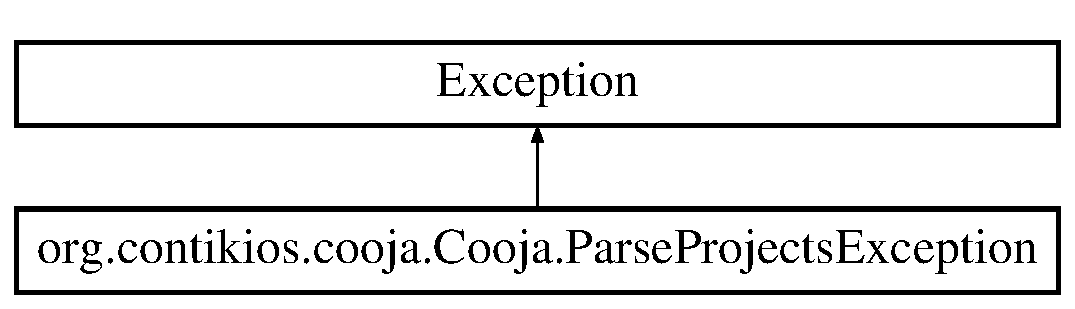
\includegraphics[height=2.000000cm]{classorg_1_1contikios_1_1cooja_1_1Cooja_1_1ParseProjectsException}
\end{center}
\end{figure}
\subsection*{Public Member Functions}
\begin{DoxyCompactItemize}
\item 
\hypertarget{classorg_1_1contikios_1_1cooja_1_1Cooja_1_1ParseProjectsException_a4647f58d68a98b1603e6648eb0510bdb}{{\bfseries Parse\-Projects\-Exception} (String message)}\label{classorg_1_1contikios_1_1cooja_1_1Cooja_1_1ParseProjectsException_a4647f58d68a98b1603e6648eb0510bdb}

\end{DoxyCompactItemize}


The documentation for this class was generated from the following file\-:\begin{DoxyCompactItemize}
\item 
Cooja.\-java\end{DoxyCompactItemize}

\hypertarget{interfaceorg_1_1contikios_1_1cooja_1_1Plugin}{\section{org.\-contikios.\-cooja.\-Plugin Interface Reference}
\label{interfaceorg_1_1contikios_1_1cooja_1_1Plugin}\index{org.\-contikios.\-cooja.\-Plugin@{org.\-contikios.\-cooja.\-Plugin}}
}
Inheritance diagram for org.\-contikios.\-cooja.\-Plugin\-:\begin{figure}[H]
\begin{center}
\leavevmode
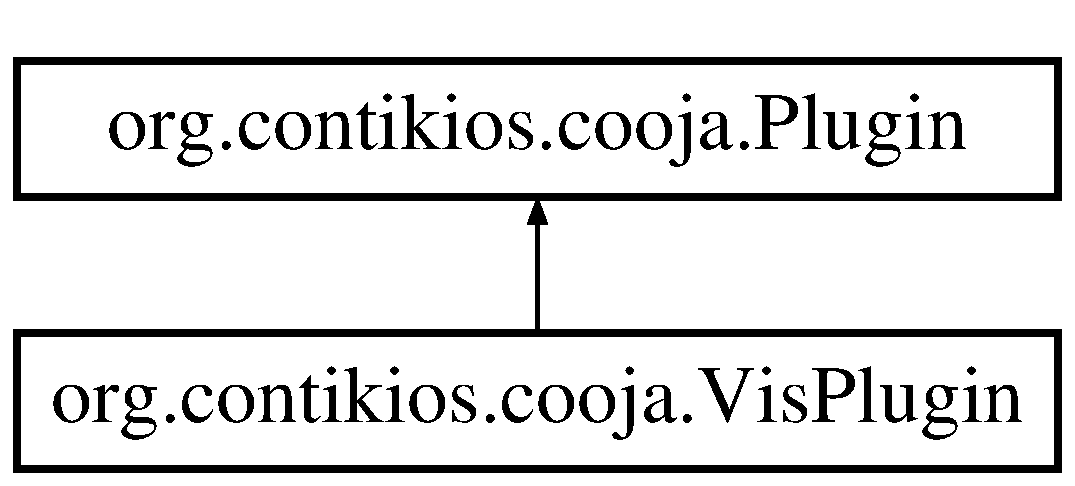
\includegraphics[height=2.000000cm]{interfaceorg_1_1contikios_1_1cooja_1_1Plugin}
\end{center}
\end{figure}
\subsection*{Public Member Functions}
\begin{DoxyCompactItemize}
\item 
J\-Internal\-Frame \hyperlink{interfaceorg_1_1contikios_1_1cooja_1_1Plugin_ae19ca3da5d492cfc80836f304f71b32a}{get\-Cooja} ()
\item 
void \hyperlink{interfaceorg_1_1contikios_1_1cooja_1_1Plugin_aae8a585e3a659cc585859a5728a42d15}{start\-Plugin} ()
\item 
void \hyperlink{interfaceorg_1_1contikios_1_1cooja_1_1Plugin_a87f92ae1a613ed6f3665a953ab748430}{close\-Plugin} ()
\item 
Collection$<$ Element $>$ \hyperlink{interfaceorg_1_1contikios_1_1cooja_1_1Plugin_acf14af975741b1de50749b358cd671a7}{get\-Config\-X\-M\-L} ()
\item 
boolean \hyperlink{interfaceorg_1_1contikios_1_1cooja_1_1Plugin_a1a7b2031b097da13170429ce7f9dc39e}{set\-Config\-X\-M\-L} (Collection$<$ Element $>$ config\-X\-M\-L, boolean vis\-Available)
\end{DoxyCompactItemize}


\subsection{Detailed Description}
C\-O\-O\-J\-A plugin. For graphical plugins, extend abstract class \hyperlink{classorg_1_1contikios_1_1cooja_1_1VisPlugin}{Vis\-Plugin}. A plugin should also use Class\-Decription and \hyperlink{interfaceorg_1_1contikios_1_1cooja_1_1PluginType}{Plugin\-Type}.

\begin{DoxySeeAlso}{See Also}
\hyperlink{interfaceorg_1_1contikios_1_1cooja_1_1ClassDescription}{org.\-contikios.\-cooja.\-Class\-Description} 

\hyperlink{interfaceorg_1_1contikios_1_1cooja_1_1PluginType}{org.\-contikios.\-cooja.\-Plugin\-Type} 

\hyperlink{classorg_1_1contikios_1_1cooja_1_1VisPlugin}{org.\-contikios.\-cooja.\-Vis\-Plugin}
\end{DoxySeeAlso}
\begin{DoxyAuthor}{Author}
Fredrik Osterlind 
\end{DoxyAuthor}


\subsection{Member Function Documentation}
\hypertarget{interfaceorg_1_1contikios_1_1cooja_1_1Plugin_a87f92ae1a613ed6f3665a953ab748430}{\index{org\-::contikios\-::cooja\-::\-Plugin@{org\-::contikios\-::cooja\-::\-Plugin}!close\-Plugin@{close\-Plugin}}
\index{close\-Plugin@{close\-Plugin}!org::contikios::cooja::Plugin@{org\-::contikios\-::cooja\-::\-Plugin}}
\subsubsection[{close\-Plugin}]{\setlength{\rightskip}{0pt plus 5cm}void org.\-contikios.\-cooja.\-Plugin.\-close\-Plugin (
\begin{DoxyParamCaption}
{}
\end{DoxyParamCaption}
)}}\label{interfaceorg_1_1contikios_1_1cooja_1_1Plugin_a87f92ae1a613ed6f3665a953ab748430}
This method is called when an opened plugin is about to close. It should release any resources such as registered observers or opened interface visualizers. 

Implemented in \hyperlink{classorg_1_1contikios_1_1cooja_1_1VisPlugin_ab010d744bcc4f590f7edd2e32e5f758d}{org.\-contikios.\-cooja.\-Vis\-Plugin}.

\hypertarget{interfaceorg_1_1contikios_1_1cooja_1_1Plugin_acf14af975741b1de50749b358cd671a7}{\index{org\-::contikios\-::cooja\-::\-Plugin@{org\-::contikios\-::cooja\-::\-Plugin}!get\-Config\-X\-M\-L@{get\-Config\-X\-M\-L}}
\index{get\-Config\-X\-M\-L@{get\-Config\-X\-M\-L}!org::contikios::cooja::Plugin@{org\-::contikios\-::cooja\-::\-Plugin}}
\subsubsection[{get\-Config\-X\-M\-L}]{\setlength{\rightskip}{0pt plus 5cm}Collection$<$Element$>$ org.\-contikios.\-cooja.\-Plugin.\-get\-Config\-X\-M\-L (
\begin{DoxyParamCaption}
{}
\end{DoxyParamCaption}
)}}\label{interfaceorg_1_1contikios_1_1cooja_1_1Plugin_acf14af975741b1de50749b358cd671a7}
Returns X\-M\-L elements representing the current config of this plugin. This is fetched by the simulator for example when saving a simulation configuration file. For example a plugin may return the current size and position. This method should however not return state specific information such as the value of a mote L\-E\-D, or total number of motes. (All nodes are restarted when loading a simulation.)

\begin{DoxySeeAlso}{See Also}
\#set\-Config\-X\-M\-L(\-Collection, boolean) 
\end{DoxySeeAlso}
\begin{DoxyReturn}{Returns}
X\-M\-L elements representing the current radio medium config 
\end{DoxyReturn}


Implemented in \hyperlink{classorg_1_1contikios_1_1cooja_1_1VisPlugin_a2c15dd2d95364a708dde19b7b54fa974}{org.\-contikios.\-cooja.\-Vis\-Plugin}.

\hypertarget{interfaceorg_1_1contikios_1_1cooja_1_1Plugin_ae19ca3da5d492cfc80836f304f71b32a}{\index{org\-::contikios\-::cooja\-::\-Plugin@{org\-::contikios\-::cooja\-::\-Plugin}!get\-Cooja@{get\-Cooja}}
\index{get\-Cooja@{get\-Cooja}!org::contikios::cooja::Plugin@{org\-::contikios\-::cooja\-::\-Plugin}}
\subsubsection[{get\-Cooja}]{\setlength{\rightskip}{0pt plus 5cm}J\-Internal\-Frame org.\-contikios.\-cooja.\-Plugin.\-get\-Cooja (
\begin{DoxyParamCaption}
{}
\end{DoxyParamCaption}
)}}\label{interfaceorg_1_1contikios_1_1cooja_1_1Plugin_ae19ca3da5d492cfc80836f304f71b32a}
Graphical component of plugin (if any) 

Implemented in \hyperlink{classorg_1_1contikios_1_1cooja_1_1VisPlugin_a4c73dd97f27405a0804a2473d3e75e35}{org.\-contikios.\-cooja.\-Vis\-Plugin}.

\hypertarget{interfaceorg_1_1contikios_1_1cooja_1_1Plugin_a1a7b2031b097da13170429ce7f9dc39e}{\index{org\-::contikios\-::cooja\-::\-Plugin@{org\-::contikios\-::cooja\-::\-Plugin}!set\-Config\-X\-M\-L@{set\-Config\-X\-M\-L}}
\index{set\-Config\-X\-M\-L@{set\-Config\-X\-M\-L}!org::contikios::cooja::Plugin@{org\-::contikios\-::cooja\-::\-Plugin}}
\subsubsection[{set\-Config\-X\-M\-L}]{\setlength{\rightskip}{0pt plus 5cm}boolean org.\-contikios.\-cooja.\-Plugin.\-set\-Config\-X\-M\-L (
\begin{DoxyParamCaption}
\item[{Collection$<$ Element $>$}]{config\-X\-M\-L, }
\item[{boolean}]{vis\-Available}
\end{DoxyParamCaption}
)}}\label{interfaceorg_1_1contikios_1_1cooja_1_1Plugin_a1a7b2031b097da13170429ce7f9dc39e}
Sets the current plugin config depending on the given X\-M\-L elements.

\begin{DoxySeeAlso}{See Also}
\hyperlink{interfaceorg_1_1contikios_1_1cooja_1_1Plugin_acf14af975741b1de50749b358cd671a7}{get\-Config\-X\-M\-L()} 
\end{DoxySeeAlso}

\begin{DoxyParams}{Parameters}
{\em config\-X\-M\-L} & Config X\-M\-L elements \\
\hline
\end{DoxyParams}
\begin{DoxyReturn}{Returns}
True if config was set successfully, false otherwise 
\end{DoxyReturn}


Implemented in \hyperlink{classorg_1_1contikios_1_1cooja_1_1VisPlugin_ad709d713ee9528c843400984ae183c6f}{org.\-contikios.\-cooja.\-Vis\-Plugin}.

\hypertarget{interfaceorg_1_1contikios_1_1cooja_1_1Plugin_aae8a585e3a659cc585859a5728a42d15}{\index{org\-::contikios\-::cooja\-::\-Plugin@{org\-::contikios\-::cooja\-::\-Plugin}!start\-Plugin@{start\-Plugin}}
\index{start\-Plugin@{start\-Plugin}!org::contikios::cooja::Plugin@{org\-::contikios\-::cooja\-::\-Plugin}}
\subsubsection[{start\-Plugin}]{\setlength{\rightskip}{0pt plus 5cm}void org.\-contikios.\-cooja.\-Plugin.\-start\-Plugin (
\begin{DoxyParamCaption}
{}
\end{DoxyParamCaption}
)}}\label{interfaceorg_1_1contikios_1_1cooja_1_1Plugin_aae8a585e3a659cc585859a5728a42d15}
This method is called to activate a new plugin, after constructing it. If a simulation is loaded, this method is called after \hyperlink{}{set\-Config\-X\-M\-L(\-Collection, boolean)}.

\begin{DoxySeeAlso}{See Also}
\#set\-Config\-X\-M\-L(\-Collection, boolean) 

\hyperlink{interfaceorg_1_1contikios_1_1cooja_1_1Plugin_a87f92ae1a613ed6f3665a953ab748430}{close\-Plugin()} 
\end{DoxySeeAlso}


Implemented in \hyperlink{classorg_1_1contikios_1_1cooja_1_1VisPlugin_a34e1bee73bd2b86e39bb267f450e624f}{org.\-contikios.\-cooja.\-Vis\-Plugin}.



The documentation for this interface was generated from the following file\-:\begin{DoxyCompactItemize}
\item 
Plugin.\-java\end{DoxyCompactItemize}

\hypertarget{classorg_1_1contikios_1_1cooja_1_1Cooja_1_1PluginConstructionException}{\section{org.\-contikios.\-cooja.\-Cooja.\-Plugin\-Construction\-Exception Class Reference}
\label{classorg_1_1contikios_1_1cooja_1_1Cooja_1_1PluginConstructionException}\index{org.\-contikios.\-cooja.\-Cooja.\-Plugin\-Construction\-Exception@{org.\-contikios.\-cooja.\-Cooja.\-Plugin\-Construction\-Exception}}
}
Inheritance diagram for org.\-contikios.\-cooja.\-Cooja.\-Plugin\-Construction\-Exception\-:\begin{figure}[H]
\begin{center}
\leavevmode
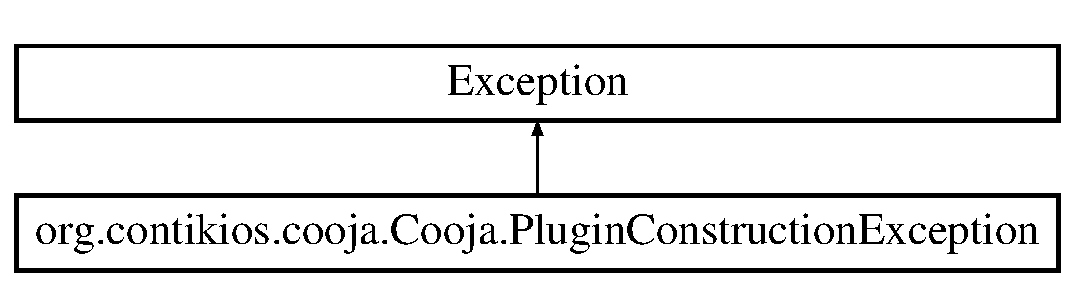
\includegraphics[height=2.000000cm]{classorg_1_1contikios_1_1cooja_1_1Cooja_1_1PluginConstructionException}
\end{center}
\end{figure}
\subsection*{Public Member Functions}
\begin{DoxyCompactItemize}
\item 
\hypertarget{classorg_1_1contikios_1_1cooja_1_1Cooja_1_1PluginConstructionException_afd8565dd04b259544a0ae5b496aacfee}{{\bfseries Plugin\-Construction\-Exception} (String message)}\label{classorg_1_1contikios_1_1cooja_1_1Cooja_1_1PluginConstructionException_afd8565dd04b259544a0ae5b496aacfee}

\end{DoxyCompactItemize}


The documentation for this class was generated from the following file\-:\begin{DoxyCompactItemize}
\item 
Cooja.\-java\end{DoxyCompactItemize}

\hypertarget{interfaceorg_1_1contikios_1_1cooja_1_1PluginType}{\section{org.\-contikios.\-cooja.\-Plugin\-Type Interface Reference}
\label{interfaceorg_1_1contikios_1_1cooja_1_1PluginType}\index{org.\-contikios.\-cooja.\-Plugin\-Type@{org.\-contikios.\-cooja.\-Plugin\-Type}}
}
\subsection*{Public Member Functions}
\begin{DoxyCompactItemize}
\item 
\hypertarget{interfaceorg_1_1contikios_1_1cooja_1_1PluginType_a0ca87dbf266adc329339e5a329b63089}{int {\bfseries value} ()}\label{interfaceorg_1_1contikios_1_1cooja_1_1PluginType_a0ca87dbf266adc329339e5a329b63089}

\end{DoxyCompactItemize}
\subsection*{Static Public Attributes}
\begin{DoxyCompactItemize}
\item 
\hypertarget{interfaceorg_1_1contikios_1_1cooja_1_1PluginType_ace254ea00f71a7f3abf76d8bb23085e4}{static final int {\bfseries U\-N\-D\-E\-F\-I\-N\-E\-D\-\_\-\-P\-L\-U\-G\-I\-N} = 0}\label{interfaceorg_1_1contikios_1_1cooja_1_1PluginType_ace254ea00f71a7f3abf76d8bb23085e4}

\item 
static final int \hyperlink{interfaceorg_1_1contikios_1_1cooja_1_1PluginType_a0feea5aed2c626e527a69fb659439478}{M\-O\-T\-E\-\_\-\-P\-L\-U\-G\-I\-N} = 1
\item 
static final int \hyperlink{interfaceorg_1_1contikios_1_1cooja_1_1PluginType_a72817595223732361a60e932965ffc24}{S\-I\-M\-\_\-\-P\-L\-U\-G\-I\-N} = 2
\item 
static final int \hyperlink{interfaceorg_1_1contikios_1_1cooja_1_1PluginType_ab27aecee60e220de3c427952226e45f8}{C\-O\-O\-J\-A\-\_\-\-P\-L\-U\-G\-I\-N} = 3
\item 
static final int \hyperlink{interfaceorg_1_1contikios_1_1cooja_1_1PluginType_a69999eed1f73b6885fb9111da26599be}{S\-I\-M\-\_\-\-S\-T\-A\-N\-D\-A\-R\-D\-\_\-\-P\-L\-U\-G\-I\-N} = 4
\item 
static final int \hyperlink{interfaceorg_1_1contikios_1_1cooja_1_1PluginType_a19f9fbc0c23f33b5decbdf6076f7b872}{C\-O\-O\-J\-A\-\_\-\-S\-T\-A\-N\-D\-A\-R\-D\-\_\-\-P\-L\-U\-G\-I\-N} = 5
\item 
static final int \hyperlink{interfaceorg_1_1contikios_1_1cooja_1_1PluginType_ae155ed8fa9ace82527925b010b33813e}{S\-I\-M\-\_\-\-C\-O\-N\-T\-R\-O\-L\-\_\-\-P\-L\-U\-G\-I\-N} = 6
\end{DoxyCompactItemize}


\subsection{Detailed Description}
Annotation type to identify a plugin type.

\begin{DoxyAuthor}{Author}
Fredrik Osterlind 
\end{DoxyAuthor}


\subsection{Member Data Documentation}
\hypertarget{interfaceorg_1_1contikios_1_1cooja_1_1PluginType_ab27aecee60e220de3c427952226e45f8}{\index{org\-::contikios\-::cooja\-::\-Plugin\-Type@{org\-::contikios\-::cooja\-::\-Plugin\-Type}!C\-O\-O\-J\-A\-\_\-\-P\-L\-U\-G\-I\-N@{C\-O\-O\-J\-A\-\_\-\-P\-L\-U\-G\-I\-N}}
\index{C\-O\-O\-J\-A\-\_\-\-P\-L\-U\-G\-I\-N@{C\-O\-O\-J\-A\-\_\-\-P\-L\-U\-G\-I\-N}!org::contikios::cooja::PluginType@{org\-::contikios\-::cooja\-::\-Plugin\-Type}}
\subsubsection[{C\-O\-O\-J\-A\-\_\-\-P\-L\-U\-G\-I\-N}]{\setlength{\rightskip}{0pt plus 5cm}final int org.\-contikios.\-cooja.\-Plugin\-Type.\-C\-O\-O\-J\-A\-\_\-\-P\-L\-U\-G\-I\-N = 3\hspace{0.3cm}{\ttfamily [static]}}}\label{interfaceorg_1_1contikios_1_1cooja_1_1PluginType_ab27aecee60e220de3c427952226e45f8}
C\-O\-O\-J\-A \hyperlink{interfaceorg_1_1contikios_1_1cooja_1_1Plugin}{Plugin}

A C\-O\-O\-J\-A plugin does not depend on the current simulation (if any).

An example of such a plugin may be a control panel where a user can save and load different simulations.

C\-O\-O\-J\-A plugins are available via the plugins menubar.

When constructed, a C\-O\-O\-J\-A plugin is given the current G\-U\-I. \hypertarget{interfaceorg_1_1contikios_1_1cooja_1_1PluginType_a19f9fbc0c23f33b5decbdf6076f7b872}{\index{org\-::contikios\-::cooja\-::\-Plugin\-Type@{org\-::contikios\-::cooja\-::\-Plugin\-Type}!C\-O\-O\-J\-A\-\_\-\-S\-T\-A\-N\-D\-A\-R\-D\-\_\-\-P\-L\-U\-G\-I\-N@{C\-O\-O\-J\-A\-\_\-\-S\-T\-A\-N\-D\-A\-R\-D\-\_\-\-P\-L\-U\-G\-I\-N}}
\index{C\-O\-O\-J\-A\-\_\-\-S\-T\-A\-N\-D\-A\-R\-D\-\_\-\-P\-L\-U\-G\-I\-N@{C\-O\-O\-J\-A\-\_\-\-S\-T\-A\-N\-D\-A\-R\-D\-\_\-\-P\-L\-U\-G\-I\-N}!org::contikios::cooja::PluginType@{org\-::contikios\-::cooja\-::\-Plugin\-Type}}
\subsubsection[{C\-O\-O\-J\-A\-\_\-\-S\-T\-A\-N\-D\-A\-R\-D\-\_\-\-P\-L\-U\-G\-I\-N}]{\setlength{\rightskip}{0pt plus 5cm}final int org.\-contikios.\-cooja.\-Plugin\-Type.\-C\-O\-O\-J\-A\-\_\-\-S\-T\-A\-N\-D\-A\-R\-D\-\_\-\-P\-L\-U\-G\-I\-N = 5\hspace{0.3cm}{\ttfamily [static]}}}\label{interfaceorg_1_1contikios_1_1cooja_1_1PluginType_a19f9fbc0c23f33b5decbdf6076f7b872}
C\-O\-O\-J\-A Standard \hyperlink{interfaceorg_1_1contikios_1_1cooja_1_1Plugin}{Plugin}

This is treated exactly like a C\-O\-O\-J\-A \hyperlink{interfaceorg_1_1contikios_1_1cooja_1_1Plugin}{Plugin}, with the only difference that this will automatically be opened when the simulator is started.

\begin{DoxySeeAlso}{See Also}
\hyperlink{interfaceorg_1_1contikios_1_1cooja_1_1PluginType_ab27aecee60e220de3c427952226e45f8}{C\-O\-O\-J\-A\-\_\-\-P\-L\-U\-G\-I\-N} 
\end{DoxySeeAlso}
\hypertarget{interfaceorg_1_1contikios_1_1cooja_1_1PluginType_a0feea5aed2c626e527a69fb659439478}{\index{org\-::contikios\-::cooja\-::\-Plugin\-Type@{org\-::contikios\-::cooja\-::\-Plugin\-Type}!M\-O\-T\-E\-\_\-\-P\-L\-U\-G\-I\-N@{M\-O\-T\-E\-\_\-\-P\-L\-U\-G\-I\-N}}
\index{M\-O\-T\-E\-\_\-\-P\-L\-U\-G\-I\-N@{M\-O\-T\-E\-\_\-\-P\-L\-U\-G\-I\-N}!org::contikios::cooja::PluginType@{org\-::contikios\-::cooja\-::\-Plugin\-Type}}
\subsubsection[{M\-O\-T\-E\-\_\-\-P\-L\-U\-G\-I\-N}]{\setlength{\rightskip}{0pt plus 5cm}final int org.\-contikios.\-cooja.\-Plugin\-Type.\-M\-O\-T\-E\-\_\-\-P\-L\-U\-G\-I\-N = 1\hspace{0.3cm}{\ttfamily [static]}}}\label{interfaceorg_1_1contikios_1_1cooja_1_1PluginType_a0feea5aed2c626e527a69fb659439478}
\hyperlink{interfaceorg_1_1contikios_1_1cooja_1_1Mote}{Mote} \hyperlink{interfaceorg_1_1contikios_1_1cooja_1_1Plugin}{Plugin}

A mote plugin concerns one specific mote.

An example of such a plugin may be to display some mote information in a frame.

\hyperlink{interfaceorg_1_1contikios_1_1cooja_1_1Mote}{Mote} plugins can not be instantiated from the regular menu bar, but are instead started from other plugins, for example a visualizer that let's a user select a mote.

When constructed, a mote plugin is given a mote, the current active simulation and the G\-U\-I object.

If the current simulation is removed, so are all instances of this plugin. \hypertarget{interfaceorg_1_1contikios_1_1cooja_1_1PluginType_ae155ed8fa9ace82527925b010b33813e}{\index{org\-::contikios\-::cooja\-::\-Plugin\-Type@{org\-::contikios\-::cooja\-::\-Plugin\-Type}!S\-I\-M\-\_\-\-C\-O\-N\-T\-R\-O\-L\-\_\-\-P\-L\-U\-G\-I\-N@{S\-I\-M\-\_\-\-C\-O\-N\-T\-R\-O\-L\-\_\-\-P\-L\-U\-G\-I\-N}}
\index{S\-I\-M\-\_\-\-C\-O\-N\-T\-R\-O\-L\-\_\-\-P\-L\-U\-G\-I\-N@{S\-I\-M\-\_\-\-C\-O\-N\-T\-R\-O\-L\-\_\-\-P\-L\-U\-G\-I\-N}!org::contikios::cooja::PluginType@{org\-::contikios\-::cooja\-::\-Plugin\-Type}}
\subsubsection[{S\-I\-M\-\_\-\-C\-O\-N\-T\-R\-O\-L\-\_\-\-P\-L\-U\-G\-I\-N}]{\setlength{\rightskip}{0pt plus 5cm}final int org.\-contikios.\-cooja.\-Plugin\-Type.\-S\-I\-M\-\_\-\-C\-O\-N\-T\-R\-O\-L\-\_\-\-P\-L\-U\-G\-I\-N = 6\hspace{0.3cm}{\ttfamily [static]}}}\label{interfaceorg_1_1contikios_1_1cooja_1_1PluginType_ae155ed8fa9ace82527925b010b33813e}
\hyperlink{classorg_1_1contikios_1_1cooja_1_1Simulation}{Simulation} Control \hyperlink{interfaceorg_1_1contikios_1_1cooja_1_1Plugin}{Plugin}

A \hyperlink{classorg_1_1contikios_1_1cooja_1_1Simulation}{Simulation} Control \hyperlink{interfaceorg_1_1contikios_1_1cooja_1_1Plugin}{Plugin} indicates control over the simulation. If C\-O\-O\-J\-A is loaded in nogui mode, it will terminate if no controll plugin is present.

C\-O\-O\-J\-A plugins are available via the plugins menubar.

When constructed, a C\-O\-O\-J\-A plugin is given the current G\-U\-I. \hypertarget{interfaceorg_1_1contikios_1_1cooja_1_1PluginType_a72817595223732361a60e932965ffc24}{\index{org\-::contikios\-::cooja\-::\-Plugin\-Type@{org\-::contikios\-::cooja\-::\-Plugin\-Type}!S\-I\-M\-\_\-\-P\-L\-U\-G\-I\-N@{S\-I\-M\-\_\-\-P\-L\-U\-G\-I\-N}}
\index{S\-I\-M\-\_\-\-P\-L\-U\-G\-I\-N@{S\-I\-M\-\_\-\-P\-L\-U\-G\-I\-N}!org::contikios::cooja::PluginType@{org\-::contikios\-::cooja\-::\-Plugin\-Type}}
\subsubsection[{S\-I\-M\-\_\-\-P\-L\-U\-G\-I\-N}]{\setlength{\rightskip}{0pt plus 5cm}final int org.\-contikios.\-cooja.\-Plugin\-Type.\-S\-I\-M\-\_\-\-P\-L\-U\-G\-I\-N = 2\hspace{0.3cm}{\ttfamily [static]}}}\label{interfaceorg_1_1contikios_1_1cooja_1_1PluginType_a72817595223732361a60e932965ffc24}
\hyperlink{classorg_1_1contikios_1_1cooja_1_1Simulation}{Simulation} \hyperlink{interfaceorg_1_1contikios_1_1cooja_1_1Plugin}{Plugin}

A simulation plugin concerns one specific simulation.

An example of such a plugin may be to display number of motes and current simulation time in a window.

\hyperlink{classorg_1_1contikios_1_1cooja_1_1Simulation}{Simulation} plugins are available via the plugins menubar.

When constructed, a simulation plugin is given the current active simulation and the G\-U\-I object.

If the current simulation is removed, so are all instances of this plugin. \hypertarget{interfaceorg_1_1contikios_1_1cooja_1_1PluginType_a69999eed1f73b6885fb9111da26599be}{\index{org\-::contikios\-::cooja\-::\-Plugin\-Type@{org\-::contikios\-::cooja\-::\-Plugin\-Type}!S\-I\-M\-\_\-\-S\-T\-A\-N\-D\-A\-R\-D\-\_\-\-P\-L\-U\-G\-I\-N@{S\-I\-M\-\_\-\-S\-T\-A\-N\-D\-A\-R\-D\-\_\-\-P\-L\-U\-G\-I\-N}}
\index{S\-I\-M\-\_\-\-S\-T\-A\-N\-D\-A\-R\-D\-\_\-\-P\-L\-U\-G\-I\-N@{S\-I\-M\-\_\-\-S\-T\-A\-N\-D\-A\-R\-D\-\_\-\-P\-L\-U\-G\-I\-N}!org::contikios::cooja::PluginType@{org\-::contikios\-::cooja\-::\-Plugin\-Type}}
\subsubsection[{S\-I\-M\-\_\-\-S\-T\-A\-N\-D\-A\-R\-D\-\_\-\-P\-L\-U\-G\-I\-N}]{\setlength{\rightskip}{0pt plus 5cm}final int org.\-contikios.\-cooja.\-Plugin\-Type.\-S\-I\-M\-\_\-\-S\-T\-A\-N\-D\-A\-R\-D\-\_\-\-P\-L\-U\-G\-I\-N = 4\hspace{0.3cm}{\ttfamily [static]}}}\label{interfaceorg_1_1contikios_1_1cooja_1_1PluginType_a69999eed1f73b6885fb9111da26599be}
\hyperlink{classorg_1_1contikios_1_1cooja_1_1Simulation}{Simulation} Standard \hyperlink{interfaceorg_1_1contikios_1_1cooja_1_1Plugin}{Plugin}

This is treated exactly like a \hyperlink{classorg_1_1contikios_1_1cooja_1_1Simulation}{Simulation} \hyperlink{interfaceorg_1_1contikios_1_1cooja_1_1Plugin}{Plugin}, with the only difference that this will automatically be opened when a new simulation is created.

\begin{DoxySeeAlso}{See Also}
\hyperlink{interfaceorg_1_1contikios_1_1cooja_1_1PluginType_a72817595223732361a60e932965ffc24}{S\-I\-M\-\_\-\-P\-L\-U\-G\-I\-N} 
\end{DoxySeeAlso}


The documentation for this interface was generated from the following file\-:\begin{DoxyCompactItemize}
\item 
Plugin\-Type.\-java\end{DoxyCompactItemize}

\hypertarget{classorg_1_1contikios_1_1cooja_1_1Positioner}{\section{org.\-contikios.\-cooja.\-Positioner Class Reference}
\label{classorg_1_1contikios_1_1cooja_1_1Positioner}\index{org.\-contikios.\-cooja.\-Positioner@{org.\-contikios.\-cooja.\-Positioner}}
}
\subsection*{Public Member Functions}
\begin{DoxyCompactItemize}
\item 
abstract double\mbox{[}$\,$\mbox{]} \hyperlink{classorg_1_1contikios_1_1cooja_1_1Positioner_a25070e5a0ec8d7a8d352e2db4c5c3902}{get\-Next\-Position} ()
\end{DoxyCompactItemize}
\subsection*{Static Public Member Functions}
\begin{DoxyCompactItemize}
\item 
static final \hyperlink{classorg_1_1contikios_1_1cooja_1_1Positioner}{Positioner} \hyperlink{classorg_1_1contikios_1_1cooja_1_1Positioner_af8c1ec799205545722307e3126098325}{generate\-Interface} (Class$<$?extends \hyperlink{classorg_1_1contikios_1_1cooja_1_1Positioner}{Positioner} $>$ positioner\-Class, int total\-Number\-Of\-Motes, double start\-X, double end\-X, double start\-Y, double end\-Y, double start\-Z, double end\-Z)
\end{DoxyCompactItemize}


\subsection{Detailed Description}
A positioner is used for determining initial positions of motes.

\begin{DoxyAuthor}{Author}
Fredrik Osterlind 
\end{DoxyAuthor}


\subsection{Member Function Documentation}
\hypertarget{classorg_1_1contikios_1_1cooja_1_1Positioner_af8c1ec799205545722307e3126098325}{\index{org\-::contikios\-::cooja\-::\-Positioner@{org\-::contikios\-::cooja\-::\-Positioner}!generate\-Interface@{generate\-Interface}}
\index{generate\-Interface@{generate\-Interface}!org::contikios::cooja::Positioner@{org\-::contikios\-::cooja\-::\-Positioner}}
\subsubsection[{generate\-Interface}]{\setlength{\rightskip}{0pt plus 5cm}static final {\bf Positioner} org.\-contikios.\-cooja.\-Positioner.\-generate\-Interface (
\begin{DoxyParamCaption}
\item[{Class$<$?extends {\bf Positioner} $>$}]{positioner\-Class, }
\item[{int}]{total\-Number\-Of\-Motes, }
\item[{double}]{start\-X, }
\item[{double}]{end\-X, }
\item[{double}]{start\-Y, }
\item[{double}]{end\-Y, }
\item[{double}]{start\-Z, }
\item[{double}]{end\-Z}
\end{DoxyParamCaption}
)\hspace{0.3cm}{\ttfamily [inline]}, {\ttfamily [static]}}}\label{classorg_1_1contikios_1_1cooja_1_1Positioner_af8c1ec799205545722307e3126098325}
This method creates an instance of the given class with the given interval information as constructor arguments. Instead of calling the constructors directly this method may be used.


\begin{DoxyParams}{Parameters}
{\em positioner\-Class} & \hyperlink{classorg_1_1contikios_1_1cooja_1_1Positioner}{Positioner} class \\
\hline
{\em total\-Number\-Of\-Motes} & Total number of motes that should be generated using this positioner \\
\hline
{\em start\-X} & Lowest X value of positions generated using returned positioner \\
\hline
{\em end\-X} & Highest X value of positions generated using returned positioner \\
\hline
{\em start\-Y} & Lowest Y value of positions generated using returned positioner \\
\hline
{\em end\-Y} & Highest Y value of positions generated using returned positioner \\
\hline
{\em start\-Z} & Lowest Z value of positions generated using returned positioner \\
\hline
{\em end\-Z} & Highest Z value of positions generated using returned positioner \\
\hline
\end{DoxyParams}
\begin{DoxyReturn}{Returns}
Postioner instance 
\end{DoxyReturn}
\hypertarget{classorg_1_1contikios_1_1cooja_1_1Positioner_a25070e5a0ec8d7a8d352e2db4c5c3902}{\index{org\-::contikios\-::cooja\-::\-Positioner@{org\-::contikios\-::cooja\-::\-Positioner}!get\-Next\-Position@{get\-Next\-Position}}
\index{get\-Next\-Position@{get\-Next\-Position}!org::contikios::cooja::Positioner@{org\-::contikios\-::cooja\-::\-Positioner}}
\subsubsection[{get\-Next\-Position}]{\setlength{\rightskip}{0pt plus 5cm}abstract double \mbox{[}$\,$\mbox{]} org.\-contikios.\-cooja.\-Positioner.\-get\-Next\-Position (
\begin{DoxyParamCaption}
{}
\end{DoxyParamCaption}
)\hspace{0.3cm}{\ttfamily [abstract]}}}\label{classorg_1_1contikios_1_1cooja_1_1Positioner_a25070e5a0ec8d7a8d352e2db4c5c3902}
Returns the next mote position.

\begin{DoxyReturn}{Returns}
Position 
\end{DoxyReturn}


The documentation for this class was generated from the following file\-:\begin{DoxyCompactItemize}
\item 
Positioner.\-java\end{DoxyCompactItemize}

\hypertarget{classorg_1_1contikios_1_1cooja_1_1ProjectConfig}{\section{org.\-contikios.\-cooja.\-Project\-Config Class Reference}
\label{classorg_1_1contikios_1_1cooja_1_1ProjectConfig}\index{org.\-contikios.\-cooja.\-Project\-Config@{org.\-contikios.\-cooja.\-Project\-Config}}
}
\subsection*{Public Member Functions}
\begin{DoxyCompactItemize}
\item 
\hyperlink{classorg_1_1contikios_1_1cooja_1_1ProjectConfig_a7ffb0811d0d278da3e5591e5ba0f142e}{Project\-Config} (boolean use\-Default)  throws I\-O\-Exception,       File\-Not\-Found\-Exception 
\item 
boolean \hyperlink{classorg_1_1contikios_1_1cooja_1_1ProjectConfig_aa536d778e7cbd7410d2eaef0996d29f3}{append\-Project\-Dir} (File project\-Dir)  throws File\-Not\-Found\-Exception, I\-O\-Exception 
\item 
File \hyperlink{classorg_1_1contikios_1_1cooja_1_1ProjectConfig_a8a4ac216a5b6a7ff3e42ad2dd4fd11a8}{get\-User\-Project\-Defining} (Class calling\-Class, String key, String array\-Element)
\item 
boolean \hyperlink{classorg_1_1contikios_1_1cooja_1_1ProjectConfig_a196e3fca713bbd57ca2ba1ffd225edf5}{append\-Config\-File} (File property\-File)  throws File\-Not\-Found\-Exception, I\-O\-Exception 
\item 
boolean \hyperlink{classorg_1_1contikios_1_1cooja_1_1ProjectConfig_aa8ad02fdc8f968aad0974d35ea529a3c}{append\-Config\-Stream} (Input\-Stream config\-File\-Stream)  throws I\-O\-Exception 
\item 
\hypertarget{classorg_1_1contikios_1_1cooja_1_1ProjectConfig_a90e9c253d8aa5e70f027cc145d3bf91b}{boolean {\bfseries append\-Config} (\hyperlink{classorg_1_1contikios_1_1cooja_1_1ProjectConfig}{Project\-Config} config)}\label{classorg_1_1contikios_1_1cooja_1_1ProjectConfig_a90e9c253d8aa5e70f027cc145d3bf91b}

\item 
Enumeration$<$ String $>$ \hyperlink{classorg_1_1contikios_1_1cooja_1_1ProjectConfig_a8e954d4b40a4af51f7851a15dd356433}{get\-Property\-Names} ()
\item 
String \hyperlink{classorg_1_1contikios_1_1cooja_1_1ProjectConfig_a21a33e307cb7b51bcd2a22cd42f20711}{get\-String\-Value} (Class calling\-Class, String id, String default\-Value)
\item 
String \hyperlink{classorg_1_1contikios_1_1cooja_1_1ProjectConfig_a9b1a075adc98af163212eb03bb1899f8}{get\-String\-Value} (String name)
\item 
String \hyperlink{classorg_1_1contikios_1_1cooja_1_1ProjectConfig_a2d9ca209d31b4a93348d4555551f49b5}{get\-String\-Value} (Class calling\-Class, String id)
\item 
String\mbox{[}$\,$\mbox{]} \hyperlink{classorg_1_1contikios_1_1cooja_1_1ProjectConfig_a240e81c9e486a5241a24ec65b4d7a772}{get\-String\-Array\-Value} (Class calling\-Class, String id)
\item 
String \hyperlink{classorg_1_1contikios_1_1cooja_1_1ProjectConfig_a9c23964b996ab25e6b4e24be5d19a6df}{get\-Value} (Class calling\-Class, String id)
\item 
String\mbox{[}$\,$\mbox{]} \hyperlink{classorg_1_1contikios_1_1cooja_1_1ProjectConfig_a022a7927422996695761bd39b7400ffc}{get\-String\-Array\-Value} (String id)
\item 
int \hyperlink{classorg_1_1contikios_1_1cooja_1_1ProjectConfig_aa63aa3e97f184949eff1ed1322cc9106}{get\-Integer\-Value} (Class calling\-Class, String id, int default\-Value)
\item 
int \hyperlink{classorg_1_1contikios_1_1cooja_1_1ProjectConfig_a326c53ca9296be299c9059bfba09c807}{get\-Integer\-Value} (Class calling\-Class, String id)
\item 
double \hyperlink{classorg_1_1contikios_1_1cooja_1_1ProjectConfig_ac0c4d039461006a06fcd743b3ee9fc6e}{get\-Double\-Value} (Class calling\-Class, String id, double default\-Value)
\item 
double \hyperlink{classorg_1_1contikios_1_1cooja_1_1ProjectConfig_a12f5d1275491768e18464c10d380f791}{get\-Double\-Value} (Class calling\-Class, String id)
\item 
boolean \hyperlink{classorg_1_1contikios_1_1cooja_1_1ProjectConfig_a457c86b3b4642729ede9e14bb850d043}{get\-Boolean\-Value} (Class calling\-Class, String id, boolean default\-Value)
\item 
boolean \hyperlink{classorg_1_1contikios_1_1cooja_1_1ProjectConfig_a9ab9cadecc9bbe636b11180a871cef11}{get\-Boolean\-Value} (Class calling\-Class, String id)
\item 
\hypertarget{classorg_1_1contikios_1_1cooja_1_1ProjectConfig_acd006795c65f6283916b6c94d8f42e06}{\hyperlink{classorg_1_1contikios_1_1cooja_1_1ProjectConfig}{Project\-Config} {\bfseries clone} ()}\label{classorg_1_1contikios_1_1cooja_1_1ProjectConfig_acd006795c65f6283916b6c94d8f42e06}

\end{DoxyCompactItemize}


\subsection{Detailed Description}
A project configuration may hold the configuration for one or several project directories as well as a general simulator configuration.

The configuration for a project directory may for example consist of which plugins, interfaces and processes that the specific project directory supplies. Each project directory configuration is read from the property file cooja.\-config, a file which is required in each project directory.

Values can be fetched as String, Boolean, Integer, Double or String array.

Several configurations can be merged, together forming a final overall configuration. The order of the how configurations are merged matter -\/ later values will overwrite earlier. For example merging two configurations with the key 'S\-O\-M\-E\-K\-E\-Y' in the following order\-:

S\-O\-M\-E\-K\-E\-Y = a b c

S\-O\-M\-E\-K\-E\-Y = d e

will result in the final value \char`\"{}d e\char`\"{}.

If a specific value should be extended instead of overwritten, the value must start with a single space-\/surrounded '+'. For example, merging two configurations with the key as above in the following order\-:

S\-O\-M\-E\-K\-E\-Y = a b c

S\-O\-M\-E\-K\-E\-Y = + d e

will result in the final value \char`\"{}a b c d e\char`\"{}.

The simulator will hold a merged project configuration, depending on which project directories are used. Additionally. each mote type may also have a configuration of its own, that differs from the general simulator configuration.

Often, but not necessarily, keys are named depending on which class is associated with the information. For example, let's say a battery interface wants to store its initial capacity (a double) using this approach. Data stored in the external configuration file can look like the following\-: org.\-contikios.\-cooja.\-interfaces.\-Battery.\-initial\-\_\-capacity 54.\-123321

This value is then be read by\-: my\-Mote\-Type\-Config.\-get\-Double\-Value(Battery.\-class, \char`\"{}initial\-\_\-capacity\char`\"{});

\begin{DoxyAuthor}{Author}
Fredrik Osterlind 
\end{DoxyAuthor}


\subsection{Constructor \& Destructor Documentation}
\hypertarget{classorg_1_1contikios_1_1cooja_1_1ProjectConfig_a7ffb0811d0d278da3e5591e5ba0f142e}{\index{org\-::contikios\-::cooja\-::\-Project\-Config@{org\-::contikios\-::cooja\-::\-Project\-Config}!Project\-Config@{Project\-Config}}
\index{Project\-Config@{Project\-Config}!org::contikios::cooja::ProjectConfig@{org\-::contikios\-::cooja\-::\-Project\-Config}}
\subsubsection[{Project\-Config}]{\setlength{\rightskip}{0pt plus 5cm}org.\-contikios.\-cooja.\-Project\-Config.\-Project\-Config (
\begin{DoxyParamCaption}
\item[{boolean}]{use\-Default}
\end{DoxyParamCaption}
) throws I\-O\-Exception,       File\-Not\-Found\-Exception\hspace{0.3cm}{\ttfamily [inline]}}}\label{classorg_1_1contikios_1_1cooja_1_1ProjectConfig_a7ffb0811d0d278da3e5591e5ba0f142e}
Creates new project configuration.


\begin{DoxyParams}{Parameters}
{\em use\-Default} & If true the default configuration will be loaded \\
\hline
\end{DoxyParams}

\begin{DoxyExceptions}{Exceptions}
{\em File\-Not\-Found\-Exception} & If file was not found \\
\hline
{\em I\-O\-Exception} & Stream read error \\
\hline
\end{DoxyExceptions}


\subsection{Member Function Documentation}
\hypertarget{classorg_1_1contikios_1_1cooja_1_1ProjectConfig_a196e3fca713bbd57ca2ba1ffd225edf5}{\index{org\-::contikios\-::cooja\-::\-Project\-Config@{org\-::contikios\-::cooja\-::\-Project\-Config}!append\-Config\-File@{append\-Config\-File}}
\index{append\-Config\-File@{append\-Config\-File}!org::contikios::cooja::ProjectConfig@{org\-::contikios\-::cooja\-::\-Project\-Config}}
\subsubsection[{append\-Config\-File}]{\setlength{\rightskip}{0pt plus 5cm}boolean org.\-contikios.\-cooja.\-Project\-Config.\-append\-Config\-File (
\begin{DoxyParamCaption}
\item[{File}]{property\-File}
\end{DoxyParamCaption}
) throws File\-Not\-Found\-Exception, I\-O\-Exception\hspace{0.3cm}{\ttfamily [inline]}}}\label{classorg_1_1contikios_1_1cooja_1_1ProjectConfig_a196e3fca713bbd57ca2ba1ffd225edf5}
Loads the given property file and appends it to the current configuration. If a property already exists it will be overwritten, unless the new value begins with a '+' in which case the old value will be extended.

W\-A\-R\-N\-I\-N\-G! The project directory history will not be saved if this method is called, instead the append\-User\-Platform method should be used.


\begin{DoxyParams}{Parameters}
{\em property\-File} & Property file to read \\
\hline
\end{DoxyParams}
\begin{DoxyReturn}{Returns}
True if file was read ok, false otherwise 
\end{DoxyReturn}

\begin{DoxyExceptions}{Exceptions}
{\em File\-Not\-Found\-Exception} & If file was not found \\
\hline
{\em I\-O\-Exception} & Stream read error \\
\hline
\end{DoxyExceptions}
\hypertarget{classorg_1_1contikios_1_1cooja_1_1ProjectConfig_aa8ad02fdc8f968aad0974d35ea529a3c}{\index{org\-::contikios\-::cooja\-::\-Project\-Config@{org\-::contikios\-::cooja\-::\-Project\-Config}!append\-Config\-Stream@{append\-Config\-Stream}}
\index{append\-Config\-Stream@{append\-Config\-Stream}!org::contikios::cooja::ProjectConfig@{org\-::contikios\-::cooja\-::\-Project\-Config}}
\subsubsection[{append\-Config\-Stream}]{\setlength{\rightskip}{0pt plus 5cm}boolean org.\-contikios.\-cooja.\-Project\-Config.\-append\-Config\-Stream (
\begin{DoxyParamCaption}
\item[{Input\-Stream}]{config\-File\-Stream}
\end{DoxyParamCaption}
) throws I\-O\-Exception\hspace{0.3cm}{\ttfamily [inline]}}}\label{classorg_1_1contikios_1_1cooja_1_1ProjectConfig_aa8ad02fdc8f968aad0974d35ea529a3c}
Reads properties from the given stream and appends them to the current configuration. If a property already exists it will be overwritten, unless the new value begins with a '+' in which case the old value will be extended.

W\-A\-R\-N\-I\-N\-G! The project directory history will not be saved if this method is called, instead the append\-User\-Platform method should be used.


\begin{DoxyParams}{Parameters}
{\em config\-File\-Stream} & Stream to read from \\
\hline
\end{DoxyParams}
\begin{DoxyReturn}{Returns}
True if stream was read ok, false otherwise 
\end{DoxyReturn}

\begin{DoxyExceptions}{Exceptions}
{\em I\-O\-Exception} & Stream read error \\
\hline
\end{DoxyExceptions}
\hypertarget{classorg_1_1contikios_1_1cooja_1_1ProjectConfig_aa536d778e7cbd7410d2eaef0996d29f3}{\index{org\-::contikios\-::cooja\-::\-Project\-Config@{org\-::contikios\-::cooja\-::\-Project\-Config}!append\-Project\-Dir@{append\-Project\-Dir}}
\index{append\-Project\-Dir@{append\-Project\-Dir}!org::contikios::cooja::ProjectConfig@{org\-::contikios\-::cooja\-::\-Project\-Config}}
\subsubsection[{append\-Project\-Dir}]{\setlength{\rightskip}{0pt plus 5cm}boolean org.\-contikios.\-cooja.\-Project\-Config.\-append\-Project\-Dir (
\begin{DoxyParamCaption}
\item[{File}]{project\-Dir}
\end{DoxyParamCaption}
) throws File\-Not\-Found\-Exception, I\-O\-Exception\hspace{0.3cm}{\ttfamily [inline]}}}\label{classorg_1_1contikios_1_1cooja_1_1ProjectConfig_aa536d778e7cbd7410d2eaef0996d29f3}
Appends the given project directory's config file. This method also saves a local history of which project directories has been loaded.


\begin{DoxyParams}{Parameters}
{\em project\-Dir} & Project directory \\
\hline
\end{DoxyParams}
\begin{DoxyReturn}{Returns}
True if loaded O\-K 
\end{DoxyReturn}

\begin{DoxyExceptions}{Exceptions}
{\em File\-Not\-Found\-Exception} & If file was not found \\
\hline
{\em I\-O\-Exception} & Stream read error \\
\hline
\end{DoxyExceptions}
\hypertarget{classorg_1_1contikios_1_1cooja_1_1ProjectConfig_a457c86b3b4642729ede9e14bb850d043}{\index{org\-::contikios\-::cooja\-::\-Project\-Config@{org\-::contikios\-::cooja\-::\-Project\-Config}!get\-Boolean\-Value@{get\-Boolean\-Value}}
\index{get\-Boolean\-Value@{get\-Boolean\-Value}!org::contikios::cooja::ProjectConfig@{org\-::contikios\-::cooja\-::\-Project\-Config}}
\subsubsection[{get\-Boolean\-Value}]{\setlength{\rightskip}{0pt plus 5cm}boolean org.\-contikios.\-cooja.\-Project\-Config.\-get\-Boolean\-Value (
\begin{DoxyParamCaption}
\item[{Class}]{calling\-Class, }
\item[{String}]{id, }
\item[{boolean}]{default\-Value}
\end{DoxyParamCaption}
)\hspace{0.3cm}{\ttfamily [inline]}}}\label{classorg_1_1contikios_1_1cooja_1_1ProjectConfig_a457c86b3b4642729ede9e14bb850d043}
Get boolean value with given id.


\begin{DoxyParams}{Parameters}
{\em calling\-Class} & Class which value belongs to \\
\hline
{\em id} & Id of value to return \\
\hline
{\em default\-Value} & Default value to return if id is not found \\
\hline
\end{DoxyParams}
\begin{DoxyReturn}{Returns}
Value or default\-Value if id wasn't found 
\end{DoxyReturn}
\hypertarget{classorg_1_1contikios_1_1cooja_1_1ProjectConfig_a9ab9cadecc9bbe636b11180a871cef11}{\index{org\-::contikios\-::cooja\-::\-Project\-Config@{org\-::contikios\-::cooja\-::\-Project\-Config}!get\-Boolean\-Value@{get\-Boolean\-Value}}
\index{get\-Boolean\-Value@{get\-Boolean\-Value}!org::contikios::cooja::ProjectConfig@{org\-::contikios\-::cooja\-::\-Project\-Config}}
\subsubsection[{get\-Boolean\-Value}]{\setlength{\rightskip}{0pt plus 5cm}boolean org.\-contikios.\-cooja.\-Project\-Config.\-get\-Boolean\-Value (
\begin{DoxyParamCaption}
\item[{Class}]{calling\-Class, }
\item[{String}]{id}
\end{DoxyParamCaption}
)\hspace{0.3cm}{\ttfamily [inline]}}}\label{classorg_1_1contikios_1_1cooja_1_1ProjectConfig_a9ab9cadecc9bbe636b11180a871cef11}
Get boolean value with given id.


\begin{DoxyParams}{Parameters}
{\em calling\-Class} & Class which value belongs to \\
\hline
{\em id} & Id of value to return \\
\hline
\end{DoxyParams}
\begin{DoxyReturn}{Returns}
Value or false if id wasn't found 
\end{DoxyReturn}
\hypertarget{classorg_1_1contikios_1_1cooja_1_1ProjectConfig_ac0c4d039461006a06fcd743b3ee9fc6e}{\index{org\-::contikios\-::cooja\-::\-Project\-Config@{org\-::contikios\-::cooja\-::\-Project\-Config}!get\-Double\-Value@{get\-Double\-Value}}
\index{get\-Double\-Value@{get\-Double\-Value}!org::contikios::cooja::ProjectConfig@{org\-::contikios\-::cooja\-::\-Project\-Config}}
\subsubsection[{get\-Double\-Value}]{\setlength{\rightskip}{0pt plus 5cm}double org.\-contikios.\-cooja.\-Project\-Config.\-get\-Double\-Value (
\begin{DoxyParamCaption}
\item[{Class}]{calling\-Class, }
\item[{String}]{id, }
\item[{double}]{default\-Value}
\end{DoxyParamCaption}
)\hspace{0.3cm}{\ttfamily [inline]}}}\label{classorg_1_1contikios_1_1cooja_1_1ProjectConfig_ac0c4d039461006a06fcd743b3ee9fc6e}
Get double value with given id.


\begin{DoxyParams}{Parameters}
{\em calling\-Class} & Class which value belongs to \\
\hline
{\em id} & Id of value to return \\
\hline
{\em default\-Value} & Default value to return if id is not found \\
\hline
\end{DoxyParams}
\begin{DoxyReturn}{Returns}
Value or default\-Value if id wasn't found 
\end{DoxyReturn}
\hypertarget{classorg_1_1contikios_1_1cooja_1_1ProjectConfig_a12f5d1275491768e18464c10d380f791}{\index{org\-::contikios\-::cooja\-::\-Project\-Config@{org\-::contikios\-::cooja\-::\-Project\-Config}!get\-Double\-Value@{get\-Double\-Value}}
\index{get\-Double\-Value@{get\-Double\-Value}!org::contikios::cooja::ProjectConfig@{org\-::contikios\-::cooja\-::\-Project\-Config}}
\subsubsection[{get\-Double\-Value}]{\setlength{\rightskip}{0pt plus 5cm}double org.\-contikios.\-cooja.\-Project\-Config.\-get\-Double\-Value (
\begin{DoxyParamCaption}
\item[{Class}]{calling\-Class, }
\item[{String}]{id}
\end{DoxyParamCaption}
)\hspace{0.3cm}{\ttfamily [inline]}}}\label{classorg_1_1contikios_1_1cooja_1_1ProjectConfig_a12f5d1275491768e18464c10d380f791}
Get double value with given id.


\begin{DoxyParams}{Parameters}
{\em calling\-Class} & Class which value belongs to \\
\hline
{\em id} & Id of value to return \\
\hline
\end{DoxyParams}
\begin{DoxyReturn}{Returns}
Value or 0.\-0 if id wasn't found 
\end{DoxyReturn}
\hypertarget{classorg_1_1contikios_1_1cooja_1_1ProjectConfig_aa63aa3e97f184949eff1ed1322cc9106}{\index{org\-::contikios\-::cooja\-::\-Project\-Config@{org\-::contikios\-::cooja\-::\-Project\-Config}!get\-Integer\-Value@{get\-Integer\-Value}}
\index{get\-Integer\-Value@{get\-Integer\-Value}!org::contikios::cooja::ProjectConfig@{org\-::contikios\-::cooja\-::\-Project\-Config}}
\subsubsection[{get\-Integer\-Value}]{\setlength{\rightskip}{0pt plus 5cm}int org.\-contikios.\-cooja.\-Project\-Config.\-get\-Integer\-Value (
\begin{DoxyParamCaption}
\item[{Class}]{calling\-Class, }
\item[{String}]{id, }
\item[{int}]{default\-Value}
\end{DoxyParamCaption}
)\hspace{0.3cm}{\ttfamily [inline]}}}\label{classorg_1_1contikios_1_1cooja_1_1ProjectConfig_aa63aa3e97f184949eff1ed1322cc9106}
Get integer value with given id.


\begin{DoxyParams}{Parameters}
{\em calling\-Class} & Class which value belongs to \\
\hline
{\em id} & Id of value to return \\
\hline
{\em default\-Value} & Default value to return if id is not found \\
\hline
\end{DoxyParams}
\begin{DoxyReturn}{Returns}
Value or default\-Value if id wasn't found 
\end{DoxyReturn}
\hypertarget{classorg_1_1contikios_1_1cooja_1_1ProjectConfig_a326c53ca9296be299c9059bfba09c807}{\index{org\-::contikios\-::cooja\-::\-Project\-Config@{org\-::contikios\-::cooja\-::\-Project\-Config}!get\-Integer\-Value@{get\-Integer\-Value}}
\index{get\-Integer\-Value@{get\-Integer\-Value}!org::contikios::cooja::ProjectConfig@{org\-::contikios\-::cooja\-::\-Project\-Config}}
\subsubsection[{get\-Integer\-Value}]{\setlength{\rightskip}{0pt plus 5cm}int org.\-contikios.\-cooja.\-Project\-Config.\-get\-Integer\-Value (
\begin{DoxyParamCaption}
\item[{Class}]{calling\-Class, }
\item[{String}]{id}
\end{DoxyParamCaption}
)\hspace{0.3cm}{\ttfamily [inline]}}}\label{classorg_1_1contikios_1_1cooja_1_1ProjectConfig_a326c53ca9296be299c9059bfba09c807}
Get integer value with given id.


\begin{DoxyParams}{Parameters}
{\em calling\-Class} & Class which value belongs to \\
\hline
{\em id} & Id of value to return \\
\hline
\end{DoxyParams}
\begin{DoxyReturn}{Returns}
Value or 0 if id wasn't found 
\end{DoxyReturn}
\hypertarget{classorg_1_1contikios_1_1cooja_1_1ProjectConfig_a8e954d4b40a4af51f7851a15dd356433}{\index{org\-::contikios\-::cooja\-::\-Project\-Config@{org\-::contikios\-::cooja\-::\-Project\-Config}!get\-Property\-Names@{get\-Property\-Names}}
\index{get\-Property\-Names@{get\-Property\-Names}!org::contikios::cooja::ProjectConfig@{org\-::contikios\-::cooja\-::\-Project\-Config}}
\subsubsection[{get\-Property\-Names}]{\setlength{\rightskip}{0pt plus 5cm}Enumeration$<$String$>$ org.\-contikios.\-cooja.\-Project\-Config.\-get\-Property\-Names (
\begin{DoxyParamCaption}
{}
\end{DoxyParamCaption}
)\hspace{0.3cm}{\ttfamily [inline]}}}\label{classorg_1_1contikios_1_1cooja_1_1ProjectConfig_a8e954d4b40a4af51f7851a15dd356433}
\begin{DoxyReturn}{Returns}
All property names in configuration 
\end{DoxyReturn}
\hypertarget{classorg_1_1contikios_1_1cooja_1_1ProjectConfig_a240e81c9e486a5241a24ec65b4d7a772}{\index{org\-::contikios\-::cooja\-::\-Project\-Config@{org\-::contikios\-::cooja\-::\-Project\-Config}!get\-String\-Array\-Value@{get\-String\-Array\-Value}}
\index{get\-String\-Array\-Value@{get\-String\-Array\-Value}!org::contikios::cooja::ProjectConfig@{org\-::contikios\-::cooja\-::\-Project\-Config}}
\subsubsection[{get\-String\-Array\-Value}]{\setlength{\rightskip}{0pt plus 5cm}String \mbox{[}$\,$\mbox{]} org.\-contikios.\-cooja.\-Project\-Config.\-get\-String\-Array\-Value (
\begin{DoxyParamCaption}
\item[{Class}]{calling\-Class, }
\item[{String}]{id}
\end{DoxyParamCaption}
)\hspace{0.3cm}{\ttfamily [inline]}}}\label{classorg_1_1contikios_1_1cooja_1_1ProjectConfig_a240e81c9e486a5241a24ec65b4d7a772}
Get string array value with given id.


\begin{DoxyParams}{Parameters}
{\em calling\-Class} & Class which value belongs to \\
\hline
{\em id} & Id of value to return \\
\hline
\end{DoxyParams}
\begin{DoxyReturn}{Returns}
Value or null if id wasn't found 
\end{DoxyReturn}
\hypertarget{classorg_1_1contikios_1_1cooja_1_1ProjectConfig_a022a7927422996695761bd39b7400ffc}{\index{org\-::contikios\-::cooja\-::\-Project\-Config@{org\-::contikios\-::cooja\-::\-Project\-Config}!get\-String\-Array\-Value@{get\-String\-Array\-Value}}
\index{get\-String\-Array\-Value@{get\-String\-Array\-Value}!org::contikios::cooja::ProjectConfig@{org\-::contikios\-::cooja\-::\-Project\-Config}}
\subsubsection[{get\-String\-Array\-Value}]{\setlength{\rightskip}{0pt plus 5cm}String \mbox{[}$\,$\mbox{]} org.\-contikios.\-cooja.\-Project\-Config.\-get\-String\-Array\-Value (
\begin{DoxyParamCaption}
\item[{String}]{id}
\end{DoxyParamCaption}
)\hspace{0.3cm}{\ttfamily [inline]}}}\label{classorg_1_1contikios_1_1cooja_1_1ProjectConfig_a022a7927422996695761bd39b7400ffc}
Get string array value with given id.


\begin{DoxyParams}{Parameters}
{\em id} & Id of value to return \\
\hline
\end{DoxyParams}
\begin{DoxyReturn}{Returns}
Value or null if id wasn't found 
\end{DoxyReturn}
\hypertarget{classorg_1_1contikios_1_1cooja_1_1ProjectConfig_a21a33e307cb7b51bcd2a22cd42f20711}{\index{org\-::contikios\-::cooja\-::\-Project\-Config@{org\-::contikios\-::cooja\-::\-Project\-Config}!get\-String\-Value@{get\-String\-Value}}
\index{get\-String\-Value@{get\-String\-Value}!org::contikios::cooja::ProjectConfig@{org\-::contikios\-::cooja\-::\-Project\-Config}}
\subsubsection[{get\-String\-Value}]{\setlength{\rightskip}{0pt plus 5cm}String org.\-contikios.\-cooja.\-Project\-Config.\-get\-String\-Value (
\begin{DoxyParamCaption}
\item[{Class}]{calling\-Class, }
\item[{String}]{id, }
\item[{String}]{default\-Value}
\end{DoxyParamCaption}
)\hspace{0.3cm}{\ttfamily [inline]}}}\label{classorg_1_1contikios_1_1cooja_1_1ProjectConfig_a21a33e307cb7b51bcd2a22cd42f20711}
Get string value with given id.


\begin{DoxyParams}{Parameters}
{\em calling\-Class} & Class which value belongs to \\
\hline
{\em id} & Id of value to return \\
\hline
{\em default\-Value} & Default value to return if id is not found \\
\hline
\end{DoxyParams}
\begin{DoxyReturn}{Returns}
Value or default\-Value if id wasn't found 
\end{DoxyReturn}
\hypertarget{classorg_1_1contikios_1_1cooja_1_1ProjectConfig_a9b1a075adc98af163212eb03bb1899f8}{\index{org\-::contikios\-::cooja\-::\-Project\-Config@{org\-::contikios\-::cooja\-::\-Project\-Config}!get\-String\-Value@{get\-String\-Value}}
\index{get\-String\-Value@{get\-String\-Value}!org::contikios::cooja::ProjectConfig@{org\-::contikios\-::cooja\-::\-Project\-Config}}
\subsubsection[{get\-String\-Value}]{\setlength{\rightskip}{0pt plus 5cm}String org.\-contikios.\-cooja.\-Project\-Config.\-get\-String\-Value (
\begin{DoxyParamCaption}
\item[{String}]{name}
\end{DoxyParamCaption}
)\hspace{0.3cm}{\ttfamily [inline]}}}\label{classorg_1_1contikios_1_1cooja_1_1ProjectConfig_a9b1a075adc98af163212eb03bb1899f8}
Returns value of given name.


\begin{DoxyParams}{Parameters}
{\em name} & Name \\
\hline
\end{DoxyParams}
\begin{DoxyReturn}{Returns}
Value as string 
\end{DoxyReturn}
\hypertarget{classorg_1_1contikios_1_1cooja_1_1ProjectConfig_a2d9ca209d31b4a93348d4555551f49b5}{\index{org\-::contikios\-::cooja\-::\-Project\-Config@{org\-::contikios\-::cooja\-::\-Project\-Config}!get\-String\-Value@{get\-String\-Value}}
\index{get\-String\-Value@{get\-String\-Value}!org::contikios::cooja::ProjectConfig@{org\-::contikios\-::cooja\-::\-Project\-Config}}
\subsubsection[{get\-String\-Value}]{\setlength{\rightskip}{0pt plus 5cm}String org.\-contikios.\-cooja.\-Project\-Config.\-get\-String\-Value (
\begin{DoxyParamCaption}
\item[{Class}]{calling\-Class, }
\item[{String}]{id}
\end{DoxyParamCaption}
)\hspace{0.3cm}{\ttfamily [inline]}}}\label{classorg_1_1contikios_1_1cooja_1_1ProjectConfig_a2d9ca209d31b4a93348d4555551f49b5}
Get string value with given id.


\begin{DoxyParams}{Parameters}
{\em calling\-Class} & Class which value belongs to \\
\hline
{\em id} & Id of value to return \\
\hline
\end{DoxyParams}
\begin{DoxyReturn}{Returns}
Value or null if id wasn't found 
\end{DoxyReturn}
\hypertarget{classorg_1_1contikios_1_1cooja_1_1ProjectConfig_a8a4ac216a5b6a7ff3e42ad2dd4fd11a8}{\index{org\-::contikios\-::cooja\-::\-Project\-Config@{org\-::contikios\-::cooja\-::\-Project\-Config}!get\-User\-Project\-Defining@{get\-User\-Project\-Defining}}
\index{get\-User\-Project\-Defining@{get\-User\-Project\-Defining}!org::contikios::cooja::ProjectConfig@{org\-::contikios\-::cooja\-::\-Project\-Config}}
\subsubsection[{get\-User\-Project\-Defining}]{\setlength{\rightskip}{0pt plus 5cm}File org.\-contikios.\-cooja.\-Project\-Config.\-get\-User\-Project\-Defining (
\begin{DoxyParamCaption}
\item[{Class}]{calling\-Class, }
\item[{String}]{key, }
\item[{String}]{array\-Element}
\end{DoxyParamCaption}
)\hspace{0.3cm}{\ttfamily [inline]}}}\label{classorg_1_1contikios_1_1cooja_1_1ProjectConfig_a8a4ac216a5b6a7ff3e42ad2dd4fd11a8}
Returns the project directory earlier appended to this configuration that defined the given key. If the key is of an array format and the given array element is non-\/null, then the project directory that added this element will be returned instead. If no such project directory can be found null is returned instead.


\begin{DoxyParams}{Parameters}
{\em calling\-Class} & Class which value belong to \\
\hline
{\em key} & Key \\
\hline
{\em array\-Element} & Value or array element \\
\hline
\end{DoxyParams}
\begin{DoxyReturn}{Returns}
Project directory defining arguments or null 
\end{DoxyReturn}
\hypertarget{classorg_1_1contikios_1_1cooja_1_1ProjectConfig_a9c23964b996ab25e6b4e24be5d19a6df}{\index{org\-::contikios\-::cooja\-::\-Project\-Config@{org\-::contikios\-::cooja\-::\-Project\-Config}!get\-Value@{get\-Value}}
\index{get\-Value@{get\-Value}!org::contikios::cooja::ProjectConfig@{org\-::contikios\-::cooja\-::\-Project\-Config}}
\subsubsection[{get\-Value}]{\setlength{\rightskip}{0pt plus 5cm}String org.\-contikios.\-cooja.\-Project\-Config.\-get\-Value (
\begin{DoxyParamCaption}
\item[{Class}]{calling\-Class, }
\item[{String}]{id}
\end{DoxyParamCaption}
)\hspace{0.3cm}{\ttfamily [inline]}}}\label{classorg_1_1contikios_1_1cooja_1_1ProjectConfig_a9c23964b996ab25e6b4e24be5d19a6df}
Get string value with given id.


\begin{DoxyParams}{Parameters}
{\em calling\-Class} & Class which value belongs to \\
\hline
{\em id} & Id of value to return \\
\hline
\end{DoxyParams}
\begin{DoxyReturn}{Returns}
Value or null if id wasn't found 
\end{DoxyReturn}


The documentation for this class was generated from the following file\-:\begin{DoxyCompactItemize}
\item 
Project\-Config.\-java\end{DoxyCompactItemize}

\hypertarget{classorg_1_1contikios_1_1cooja_1_1RadioConnection}{\section{org.\-contikios.\-cooja.\-Radio\-Connection Class Reference}
\label{classorg_1_1contikios_1_1cooja_1_1RadioConnection}\index{org.\-contikios.\-cooja.\-Radio\-Connection@{org.\-contikios.\-cooja.\-Radio\-Connection}}
}
\subsection*{Public Member Functions}
\begin{DoxyCompactItemize}
\item 
\hyperlink{classorg_1_1contikios_1_1cooja_1_1RadioConnection_adeb449c52aa586de0b34c14b8c6ead39}{Radio\-Connection} (Radio source\-Radio)
\item 
long \hyperlink{classorg_1_1contikios_1_1cooja_1_1RadioConnection_ab334a3820d0405a0b2b6aa7683561149}{get\-Start\-Time} ()
\item 
long \hyperlink{classorg_1_1contikios_1_1cooja_1_1RadioConnection_af2bd3c40fa297d883ccb1d2285b0edd1}{get\-Reception\-Start\-Time} ()
\item 
void \hyperlink{classorg_1_1contikios_1_1cooja_1_1RadioConnection_a7faeaa8de29ad4f8499540d0a38a0c4b}{add\-Destination} (Radio radio)
\item 
void \hyperlink{classorg_1_1contikios_1_1cooja_1_1RadioConnection_a988eb4ce5c7a4fcac7a535134c11d2a8}{remove\-Destination} (Radio radio)
\item 
void \hyperlink{classorg_1_1contikios_1_1cooja_1_1RadioConnection_a83d1396b6ef027e9c795777deff20d11}{add\-Destination} (Radio radio, Long delay)
\item 
long \hyperlink{classorg_1_1contikios_1_1cooja_1_1RadioConnection_ac2b68a135d0452a53561609d8c5aa943}{get\-Destination\-Delay} (Radio radio)
\item 
void \hyperlink{classorg_1_1contikios_1_1cooja_1_1RadioConnection_acaff68ac6d8f5dc265c2a51e9a7439bc}{add\-Interfered} (Radio radio)
\item 
boolean \hyperlink{classorg_1_1contikios_1_1cooja_1_1RadioConnection_aea0b41548059472407b9c33fa62734ea}{is\-Destination} (Radio radio)
\item 
boolean \hyperlink{classorg_1_1contikios_1_1cooja_1_1RadioConnection_a4a0dfb86d28970240ddd53132c24d300}{is\-Interfered} (Radio radio)
\item 
Radio \hyperlink{classorg_1_1contikios_1_1cooja_1_1RadioConnection_aa360f2c130d032769b2d78c895041c71}{get\-Source} ()
\item 
Radio\mbox{[}$\,$\mbox{]} \hyperlink{classorg_1_1contikios_1_1cooja_1_1RadioConnection_ad58d2f1f7529dfc6fb5fb573c666875a}{get\-Destinations} ()
\item 
Radio\mbox{[}$\,$\mbox{]} \hyperlink{classorg_1_1contikios_1_1cooja_1_1RadioConnection_abe5029d3e9dfed7d4d83994bf706c2c9}{get\-All\-Destinations} ()
\item 
Radio\mbox{[}$\,$\mbox{]} \hyperlink{classorg_1_1contikios_1_1cooja_1_1RadioConnection_a51a86f77fa9cea56aa1333c71bd7b20a}{get\-Interfered} ()
\item 
\hypertarget{classorg_1_1contikios_1_1cooja_1_1RadioConnection_a73d8be903af6e728425b3ae5aa1ce308}{Radio\mbox{[}$\,$\mbox{]} {\bfseries get\-Interfered\-Non\-Destinations} ()}\label{classorg_1_1contikios_1_1cooja_1_1RadioConnection_a73d8be903af6e728425b3ae5aa1ce308}

\item 
\hypertarget{classorg_1_1contikios_1_1cooja_1_1RadioConnection_adda2c2eb516d11a34c4597e4eea1f17a}{String {\bfseries to\-String} ()}\label{classorg_1_1contikios_1_1cooja_1_1RadioConnection_adda2c2eb516d11a34c4597e4eea1f17a}

\end{DoxyCompactItemize}


\subsection{Detailed Description}
A radio connection represents a connection between a single source radio and any number of destination and interfered radios.

Note that a destination node may be interfered, and that an interfered radio does not need to be a destination. Interfered radios may be added during the connection lifetime.

Radio medium implementations may differ slightly in how they forward connection data to destination and interfered radios. Typically, however, all destination radios (including those that are interfered) receive the connection data. And the interfered non-\/destination radios do not receive the connection data.

\begin{DoxySeeAlso}{See Also}
\hyperlink{classorg_1_1contikios_1_1cooja_1_1RadioMedium}{Radio\-Medium} 
\end{DoxySeeAlso}
\begin{DoxyAuthor}{Author}
Fredrik Osterlind 
\end{DoxyAuthor}


\subsection{Constructor \& Destructor Documentation}
\hypertarget{classorg_1_1contikios_1_1cooja_1_1RadioConnection_adeb449c52aa586de0b34c14b8c6ead39}{\index{org\-::contikios\-::cooja\-::\-Radio\-Connection@{org\-::contikios\-::cooja\-::\-Radio\-Connection}!Radio\-Connection@{Radio\-Connection}}
\index{Radio\-Connection@{Radio\-Connection}!org::contikios::cooja::RadioConnection@{org\-::contikios\-::cooja\-::\-Radio\-Connection}}
\subsubsection[{Radio\-Connection}]{\setlength{\rightskip}{0pt plus 5cm}org.\-contikios.\-cooja.\-Radio\-Connection.\-Radio\-Connection (
\begin{DoxyParamCaption}
\item[{Radio}]{source\-Radio}
\end{DoxyParamCaption}
)\hspace{0.3cm}{\ttfamily [inline]}}}\label{classorg_1_1contikios_1_1cooja_1_1RadioConnection_adeb449c52aa586de0b34c14b8c6ead39}
Creates a new radio connection with given source and no destinations.


\begin{DoxyParams}{Parameters}
{\em source\-Radio} & Source radio \\
\hline
\end{DoxyParams}


\subsection{Member Function Documentation}
\hypertarget{classorg_1_1contikios_1_1cooja_1_1RadioConnection_a7faeaa8de29ad4f8499540d0a38a0c4b}{\index{org\-::contikios\-::cooja\-::\-Radio\-Connection@{org\-::contikios\-::cooja\-::\-Radio\-Connection}!add\-Destination@{add\-Destination}}
\index{add\-Destination@{add\-Destination}!org::contikios::cooja::RadioConnection@{org\-::contikios\-::cooja\-::\-Radio\-Connection}}
\subsubsection[{add\-Destination}]{\setlength{\rightskip}{0pt plus 5cm}void org.\-contikios.\-cooja.\-Radio\-Connection.\-add\-Destination (
\begin{DoxyParamCaption}
\item[{Radio}]{radio}
\end{DoxyParamCaption}
)\hspace{0.3cm}{\ttfamily [inline]}}}\label{classorg_1_1contikios_1_1cooja_1_1RadioConnection_a7faeaa8de29ad4f8499540d0a38a0c4b}
Add (non-\/interfered) destination radio to connection.


\begin{DoxyParams}{Parameters}
{\em radio} & Radio \\
\hline
\end{DoxyParams}
\hypertarget{classorg_1_1contikios_1_1cooja_1_1RadioConnection_a83d1396b6ef027e9c795777deff20d11}{\index{org\-::contikios\-::cooja\-::\-Radio\-Connection@{org\-::contikios\-::cooja\-::\-Radio\-Connection}!add\-Destination@{add\-Destination}}
\index{add\-Destination@{add\-Destination}!org::contikios::cooja::RadioConnection@{org\-::contikios\-::cooja\-::\-Radio\-Connection}}
\subsubsection[{add\-Destination}]{\setlength{\rightskip}{0pt plus 5cm}void org.\-contikios.\-cooja.\-Radio\-Connection.\-add\-Destination (
\begin{DoxyParamCaption}
\item[{Radio}]{radio, }
\item[{Long}]{delay}
\end{DoxyParamCaption}
)\hspace{0.3cm}{\ttfamily [inline]}}}\label{classorg_1_1contikios_1_1cooja_1_1RadioConnection_a83d1396b6ef027e9c795777deff20d11}
Add (non-\/interfered) destination radio to connection.


\begin{DoxyParams}{Parameters}
{\em radio} & Radio \\
\hline
{\em delay} & Radio propagation delay (us) \\
\hline
\end{DoxyParams}
\hypertarget{classorg_1_1contikios_1_1cooja_1_1RadioConnection_acaff68ac6d8f5dc265c2a51e9a7439bc}{\index{org\-::contikios\-::cooja\-::\-Radio\-Connection@{org\-::contikios\-::cooja\-::\-Radio\-Connection}!add\-Interfered@{add\-Interfered}}
\index{add\-Interfered@{add\-Interfered}!org::contikios::cooja::RadioConnection@{org\-::contikios\-::cooja\-::\-Radio\-Connection}}
\subsubsection[{add\-Interfered}]{\setlength{\rightskip}{0pt plus 5cm}void org.\-contikios.\-cooja.\-Radio\-Connection.\-add\-Interfered (
\begin{DoxyParamCaption}
\item[{Radio}]{radio}
\end{DoxyParamCaption}
)\hspace{0.3cm}{\ttfamily [inline]}}}\label{classorg_1_1contikios_1_1cooja_1_1RadioConnection_acaff68ac6d8f5dc265c2a51e9a7439bc}
Adds interfered radio to connection. Note that the radio may or may not already be a destination.


\begin{DoxyParams}{Parameters}
{\em radio} & Radio \\
\hline
\end{DoxyParams}
\begin{DoxySeeAlso}{See Also}
\hyperlink{classorg_1_1contikios_1_1cooja_1_1RadioConnection_ad58d2f1f7529dfc6fb5fb573c666875a}{get\-Destinations()} 

\hyperlink{classorg_1_1contikios_1_1cooja_1_1RadioConnection_abe5029d3e9dfed7d4d83994bf706c2c9}{get\-All\-Destinations()} 
\end{DoxySeeAlso}
\hypertarget{classorg_1_1contikios_1_1cooja_1_1RadioConnection_abe5029d3e9dfed7d4d83994bf706c2c9}{\index{org\-::contikios\-::cooja\-::\-Radio\-Connection@{org\-::contikios\-::cooja\-::\-Radio\-Connection}!get\-All\-Destinations@{get\-All\-Destinations}}
\index{get\-All\-Destinations@{get\-All\-Destinations}!org::contikios::cooja::RadioConnection@{org\-::contikios\-::cooja\-::\-Radio\-Connection}}
\subsubsection[{get\-All\-Destinations}]{\setlength{\rightskip}{0pt plus 5cm}Radio \mbox{[}$\,$\mbox{]} org.\-contikios.\-cooja.\-Radio\-Connection.\-get\-All\-Destinations (
\begin{DoxyParamCaption}
{}
\end{DoxyParamCaption}
)\hspace{0.3cm}{\ttfamily [inline]}}}\label{classorg_1_1contikios_1_1cooja_1_1RadioConnection_abe5029d3e9dfed7d4d83994bf706c2c9}
\begin{DoxySeeAlso}{See Also}
\hyperlink{classorg_1_1contikios_1_1cooja_1_1RadioConnection_ad58d2f1f7529dfc6fb5fb573c666875a}{get\-Destinations()} 
\end{DoxySeeAlso}
\begin{DoxyReturn}{Returns}
All destination radios, including radios that became interfered after the connection started. 
\end{DoxyReturn}
\hypertarget{classorg_1_1contikios_1_1cooja_1_1RadioConnection_ac2b68a135d0452a53561609d8c5aa943}{\index{org\-::contikios\-::cooja\-::\-Radio\-Connection@{org\-::contikios\-::cooja\-::\-Radio\-Connection}!get\-Destination\-Delay@{get\-Destination\-Delay}}
\index{get\-Destination\-Delay@{get\-Destination\-Delay}!org::contikios::cooja::RadioConnection@{org\-::contikios\-::cooja\-::\-Radio\-Connection}}
\subsubsection[{get\-Destination\-Delay}]{\setlength{\rightskip}{0pt plus 5cm}long org.\-contikios.\-cooja.\-Radio\-Connection.\-get\-Destination\-Delay (
\begin{DoxyParamCaption}
\item[{Radio}]{radio}
\end{DoxyParamCaption}
)\hspace{0.3cm}{\ttfamily [inline]}}}\label{classorg_1_1contikios_1_1cooja_1_1RadioConnection_ac2b68a135d0452a53561609d8c5aa943}

\begin{DoxyParams}{Parameters}
{\em radio} & Radio \\
\hline
\end{DoxyParams}
\begin{DoxyReturn}{Returns}
Radio propagation delay (us) 
\end{DoxyReturn}
\hypertarget{classorg_1_1contikios_1_1cooja_1_1RadioConnection_ad58d2f1f7529dfc6fb5fb573c666875a}{\index{org\-::contikios\-::cooja\-::\-Radio\-Connection@{org\-::contikios\-::cooja\-::\-Radio\-Connection}!get\-Destinations@{get\-Destinations}}
\index{get\-Destinations@{get\-Destinations}!org::contikios::cooja::RadioConnection@{org\-::contikios\-::cooja\-::\-Radio\-Connection}}
\subsubsection[{get\-Destinations}]{\setlength{\rightskip}{0pt plus 5cm}Radio \mbox{[}$\,$\mbox{]} org.\-contikios.\-cooja.\-Radio\-Connection.\-get\-Destinations (
\begin{DoxyParamCaption}
{}
\end{DoxyParamCaption}
)\hspace{0.3cm}{\ttfamily [inline]}}}\label{classorg_1_1contikios_1_1cooja_1_1RadioConnection_ad58d2f1f7529dfc6fb5fb573c666875a}
\begin{DoxySeeAlso}{See Also}
\hyperlink{classorg_1_1contikios_1_1cooja_1_1RadioConnection_abe5029d3e9dfed7d4d83994bf706c2c9}{get\-All\-Destinations()} 
\end{DoxySeeAlso}
\begin{DoxyReturn}{Returns}
All non-\/interfered destinations 
\end{DoxyReturn}
\hypertarget{classorg_1_1contikios_1_1cooja_1_1RadioConnection_a51a86f77fa9cea56aa1333c71bd7b20a}{\index{org\-::contikios\-::cooja\-::\-Radio\-Connection@{org\-::contikios\-::cooja\-::\-Radio\-Connection}!get\-Interfered@{get\-Interfered}}
\index{get\-Interfered@{get\-Interfered}!org::contikios::cooja::RadioConnection@{org\-::contikios\-::cooja\-::\-Radio\-Connection}}
\subsubsection[{get\-Interfered}]{\setlength{\rightskip}{0pt plus 5cm}Radio \mbox{[}$\,$\mbox{]} org.\-contikios.\-cooja.\-Radio\-Connection.\-get\-Interfered (
\begin{DoxyParamCaption}
{}
\end{DoxyParamCaption}
)\hspace{0.3cm}{\ttfamily [inline]}}}\label{classorg_1_1contikios_1_1cooja_1_1RadioConnection_a51a86f77fa9cea56aa1333c71bd7b20a}
\begin{DoxyReturn}{Returns}
All radios interfered by this connection, including destinations 
\end{DoxyReturn}
\hypertarget{classorg_1_1contikios_1_1cooja_1_1RadioConnection_af2bd3c40fa297d883ccb1d2285b0edd1}{\index{org\-::contikios\-::cooja\-::\-Radio\-Connection@{org\-::contikios\-::cooja\-::\-Radio\-Connection}!get\-Reception\-Start\-Time@{get\-Reception\-Start\-Time}}
\index{get\-Reception\-Start\-Time@{get\-Reception\-Start\-Time}!org::contikios::cooja::RadioConnection@{org\-::contikios\-::cooja\-::\-Radio\-Connection}}
\subsubsection[{get\-Reception\-Start\-Time}]{\setlength{\rightskip}{0pt plus 5cm}long org.\-contikios.\-cooja.\-Radio\-Connection.\-get\-Reception\-Start\-Time (
\begin{DoxyParamCaption}
{}
\end{DoxyParamCaption}
)\hspace{0.3cm}{\ttfamily [inline]}}}\label{classorg_1_1contikios_1_1cooja_1_1RadioConnection_af2bd3c40fa297d883ccb1d2285b0edd1}
\begin{DoxyReturn}{Returns}
Start time of ongoing reception 
\end{DoxyReturn}
\hypertarget{classorg_1_1contikios_1_1cooja_1_1RadioConnection_aa360f2c130d032769b2d78c895041c71}{\index{org\-::contikios\-::cooja\-::\-Radio\-Connection@{org\-::contikios\-::cooja\-::\-Radio\-Connection}!get\-Source@{get\-Source}}
\index{get\-Source@{get\-Source}!org::contikios::cooja::RadioConnection@{org\-::contikios\-::cooja\-::\-Radio\-Connection}}
\subsubsection[{get\-Source}]{\setlength{\rightskip}{0pt plus 5cm}Radio org.\-contikios.\-cooja.\-Radio\-Connection.\-get\-Source (
\begin{DoxyParamCaption}
{}
\end{DoxyParamCaption}
)\hspace{0.3cm}{\ttfamily [inline]}}}\label{classorg_1_1contikios_1_1cooja_1_1RadioConnection_aa360f2c130d032769b2d78c895041c71}
\begin{DoxyReturn}{Returns}
Source radio 
\end{DoxyReturn}
\hypertarget{classorg_1_1contikios_1_1cooja_1_1RadioConnection_ab334a3820d0405a0b2b6aa7683561149}{\index{org\-::contikios\-::cooja\-::\-Radio\-Connection@{org\-::contikios\-::cooja\-::\-Radio\-Connection}!get\-Start\-Time@{get\-Start\-Time}}
\index{get\-Start\-Time@{get\-Start\-Time}!org::contikios::cooja::RadioConnection@{org\-::contikios\-::cooja\-::\-Radio\-Connection}}
\subsubsection[{get\-Start\-Time}]{\setlength{\rightskip}{0pt plus 5cm}long org.\-contikios.\-cooja.\-Radio\-Connection.\-get\-Start\-Time (
\begin{DoxyParamCaption}
{}
\end{DoxyParamCaption}
)\hspace{0.3cm}{\ttfamily [inline]}}}\label{classorg_1_1contikios_1_1cooja_1_1RadioConnection_ab334a3820d0405a0b2b6aa7683561149}
\begin{DoxyReturn}{Returns}
Radio connection start time 
\end{DoxyReturn}
\hypertarget{classorg_1_1contikios_1_1cooja_1_1RadioConnection_aea0b41548059472407b9c33fa62734ea}{\index{org\-::contikios\-::cooja\-::\-Radio\-Connection@{org\-::contikios\-::cooja\-::\-Radio\-Connection}!is\-Destination@{is\-Destination}}
\index{is\-Destination@{is\-Destination}!org::contikios::cooja::RadioConnection@{org\-::contikios\-::cooja\-::\-Radio\-Connection}}
\subsubsection[{is\-Destination}]{\setlength{\rightskip}{0pt plus 5cm}boolean org.\-contikios.\-cooja.\-Radio\-Connection.\-is\-Destination (
\begin{DoxyParamCaption}
\item[{Radio}]{radio}
\end{DoxyParamCaption}
)\hspace{0.3cm}{\ttfamily [inline]}}}\label{classorg_1_1contikios_1_1cooja_1_1RadioConnection_aea0b41548059472407b9c33fa62734ea}

\begin{DoxyParams}{Parameters}
{\em radio} & Radio \\
\hline
\end{DoxyParams}
\begin{DoxyReturn}{Returns}
True if radio is a non-\/interfered destination in this connection 
\end{DoxyReturn}
\hypertarget{classorg_1_1contikios_1_1cooja_1_1RadioConnection_a4a0dfb86d28970240ddd53132c24d300}{\index{org\-::contikios\-::cooja\-::\-Radio\-Connection@{org\-::contikios\-::cooja\-::\-Radio\-Connection}!is\-Interfered@{is\-Interfered}}
\index{is\-Interfered@{is\-Interfered}!org::contikios::cooja::RadioConnection@{org\-::contikios\-::cooja\-::\-Radio\-Connection}}
\subsubsection[{is\-Interfered}]{\setlength{\rightskip}{0pt plus 5cm}boolean org.\-contikios.\-cooja.\-Radio\-Connection.\-is\-Interfered (
\begin{DoxyParamCaption}
\item[{Radio}]{radio}
\end{DoxyParamCaption}
)\hspace{0.3cm}{\ttfamily [inline]}}}\label{classorg_1_1contikios_1_1cooja_1_1RadioConnection_a4a0dfb86d28970240ddd53132c24d300}

\begin{DoxyParams}{Parameters}
{\em radio} & Radio \\
\hline
\end{DoxyParams}
\begin{DoxyReturn}{Returns}
True if radio is interfered in this connection 
\end{DoxyReturn}
\hypertarget{classorg_1_1contikios_1_1cooja_1_1RadioConnection_a988eb4ce5c7a4fcac7a535134c11d2a8}{\index{org\-::contikios\-::cooja\-::\-Radio\-Connection@{org\-::contikios\-::cooja\-::\-Radio\-Connection}!remove\-Destination@{remove\-Destination}}
\index{remove\-Destination@{remove\-Destination}!org::contikios::cooja::RadioConnection@{org\-::contikios\-::cooja\-::\-Radio\-Connection}}
\subsubsection[{remove\-Destination}]{\setlength{\rightskip}{0pt plus 5cm}void org.\-contikios.\-cooja.\-Radio\-Connection.\-remove\-Destination (
\begin{DoxyParamCaption}
\item[{Radio}]{radio}
\end{DoxyParamCaption}
)\hspace{0.3cm}{\ttfamily [inline]}}}\label{classorg_1_1contikios_1_1cooja_1_1RadioConnection_a988eb4ce5c7a4fcac7a535134c11d2a8}
Experimental\-: remove destination.


\begin{DoxyParams}{Parameters}
{\em radio} & Radio \\
\hline
\end{DoxyParams}


The documentation for this class was generated from the following file\-:\begin{DoxyCompactItemize}
\item 
Radio\-Connection.\-java\end{DoxyCompactItemize}

\hypertarget{classorg_1_1contikios_1_1cooja_1_1RadioMedium}{\section{org.\-contikios.\-cooja.\-Radio\-Medium Class Reference}
\label{classorg_1_1contikios_1_1cooja_1_1RadioMedium}\index{org.\-contikios.\-cooja.\-Radio\-Medium@{org.\-contikios.\-cooja.\-Radio\-Medium}}
}
\subsection*{Public Member Functions}
\begin{DoxyCompactItemize}
\item 
abstract void \hyperlink{classorg_1_1contikios_1_1cooja_1_1RadioMedium_a39920abebfaeb932d81f000105c82840}{register\-Mote} (\hyperlink{interfaceorg_1_1contikios_1_1cooja_1_1Mote}{Mote} mote, \hyperlink{classorg_1_1contikios_1_1cooja_1_1Simulation}{Simulation} sim)
\item 
abstract void \hyperlink{classorg_1_1contikios_1_1cooja_1_1RadioMedium_a806edffedd9606780fe56939fa725d80}{unregister\-Mote} (\hyperlink{interfaceorg_1_1contikios_1_1cooja_1_1Mote}{Mote} mote, \hyperlink{classorg_1_1contikios_1_1cooja_1_1Simulation}{Simulation} sim)
\item 
abstract void \hyperlink{classorg_1_1contikios_1_1cooja_1_1RadioMedium_a81b6c3a9c65b25b22ea1873a9e86fc98}{register\-Radio\-Interface} (Radio radio, \hyperlink{classorg_1_1contikios_1_1cooja_1_1Simulation}{Simulation} sim)
\item 
abstract void \hyperlink{classorg_1_1contikios_1_1cooja_1_1RadioMedium_ab51a23482434fc03797ccdb07f296907}{unregister\-Radio\-Interface} (Radio radio, \hyperlink{classorg_1_1contikios_1_1cooja_1_1Simulation}{Simulation} sim)
\item 
abstract void \hyperlink{classorg_1_1contikios_1_1cooja_1_1RadioMedium_af9064dbe7a700b6d3a8c04b1b8d671b8}{add\-Radio\-Medium\-Observer} (Observer observer)
\item 
abstract Observable \hyperlink{classorg_1_1contikios_1_1cooja_1_1RadioMedium_a5afe3150f3cec816ff0a8bae5e23b3db}{get\-Radio\-Medium\-Observable} ()
\item 
abstract void \hyperlink{classorg_1_1contikios_1_1cooja_1_1RadioMedium_a6d7e1bb0b233bb7040d19376ff861a3c}{delete\-Radio\-Medium\-Observer} (Observer observer)
\item 
abstract \hyperlink{classorg_1_1contikios_1_1cooja_1_1RadioConnection}{Radio\-Connection} \hyperlink{classorg_1_1contikios_1_1cooja_1_1RadioMedium_aa260c46b107c56d6dcb38c3402828bca}{get\-Last\-Connection} ()
\item 
abstract Collection$<$ Element $>$ \hyperlink{classorg_1_1contikios_1_1cooja_1_1RadioMedium_a7029597231ff6a8f9f3fadc2c4d1c42c}{get\-Config\-X\-M\-L} ()
\item 
abstract boolean \hyperlink{classorg_1_1contikios_1_1cooja_1_1RadioMedium_ad254dbb634c35f33b2ee13597d14aa58}{set\-Config\-X\-M\-L} (Collection$<$ Element $>$ config\-X\-M\-L, boolean vis\-Available)
\item 
void \hyperlink{classorg_1_1contikios_1_1cooja_1_1RadioMedium_a91b2afc1b3dcf7f558e36eff4b3bc52b}{removed} ()
\item 
void \hyperlink{classorg_1_1contikios_1_1cooja_1_1RadioMedium_a75c1d2997520c3ad7ce190c73a484ef9}{simulation\-Finished\-Loading} ()
\end{DoxyCompactItemize}
\subsection*{Static Public Member Functions}
\begin{DoxyCompactItemize}
\item 
static final \hyperlink{classorg_1_1contikios_1_1cooja_1_1RadioMedium}{Radio\-Medium} \hyperlink{classorg_1_1contikios_1_1cooja_1_1RadioMedium_a92344f72831d4470231ac63757d8b8f5}{generate\-Radio\-Medium} (Class$<$?extends \hyperlink{classorg_1_1contikios_1_1cooja_1_1RadioMedium}{Radio\-Medium} $>$ radio\-Medium\-Class, \hyperlink{classorg_1_1contikios_1_1cooja_1_1Simulation}{Simulation} simulation)  throws No\-Such\-Method\-Exception, Invocation\-Target\-Exception,       Illegal\-Access\-Exception, Instantiation\-Exception 
\end{DoxyCompactItemize}


\subsection{Detailed Description}
The abstract class \hyperlink{classorg_1_1contikios_1_1cooja_1_1RadioMedium}{Radio\-Medium} should be implemented by all C\-O\-O\-J\-A radio mediums. Radios registered in this medium can both send and receive radio data. Depending on the implementation of this interface, more or less accurate radio behaviour imitation is aquired.

\begin{DoxyAuthor}{Author}
Fredrik Osterlind 
\end{DoxyAuthor}


\subsection{Member Function Documentation}
\hypertarget{classorg_1_1contikios_1_1cooja_1_1RadioMedium_af9064dbe7a700b6d3a8c04b1b8d671b8}{\index{org\-::contikios\-::cooja\-::\-Radio\-Medium@{org\-::contikios\-::cooja\-::\-Radio\-Medium}!add\-Radio\-Medium\-Observer@{add\-Radio\-Medium\-Observer}}
\index{add\-Radio\-Medium\-Observer@{add\-Radio\-Medium\-Observer}!org::contikios::cooja::RadioMedium@{org\-::contikios\-::cooja\-::\-Radio\-Medium}}
\subsubsection[{add\-Radio\-Medium\-Observer}]{\setlength{\rightskip}{0pt plus 5cm}abstract void org.\-contikios.\-cooja.\-Radio\-Medium.\-add\-Radio\-Medium\-Observer (
\begin{DoxyParamCaption}
\item[{Observer}]{observer}
\end{DoxyParamCaption}
)\hspace{0.3cm}{\ttfamily [abstract]}}}\label{classorg_1_1contikios_1_1cooja_1_1RadioMedium_af9064dbe7a700b6d3a8c04b1b8d671b8}
Adds an observer which is notified each time a radio connection has finished.

\begin{DoxySeeAlso}{See Also}
\hyperlink{classorg_1_1contikios_1_1cooja_1_1RadioMedium_aa260c46b107c56d6dcb38c3402828bca}{get\-Last\-Connection()} 

\hyperlink{classorg_1_1contikios_1_1cooja_1_1RadioMedium_a6d7e1bb0b233bb7040d19376ff861a3c}{delete\-Radio\-Medium\-Observer(\-Observer)} 
\end{DoxySeeAlso}

\begin{DoxyParams}{Parameters}
{\em observer} & New observer \\
\hline
\end{DoxyParams}
\hypertarget{classorg_1_1contikios_1_1cooja_1_1RadioMedium_a6d7e1bb0b233bb7040d19376ff861a3c}{\index{org\-::contikios\-::cooja\-::\-Radio\-Medium@{org\-::contikios\-::cooja\-::\-Radio\-Medium}!delete\-Radio\-Medium\-Observer@{delete\-Radio\-Medium\-Observer}}
\index{delete\-Radio\-Medium\-Observer@{delete\-Radio\-Medium\-Observer}!org::contikios::cooja::RadioMedium@{org\-::contikios\-::cooja\-::\-Radio\-Medium}}
\subsubsection[{delete\-Radio\-Medium\-Observer}]{\setlength{\rightskip}{0pt plus 5cm}abstract void org.\-contikios.\-cooja.\-Radio\-Medium.\-delete\-Radio\-Medium\-Observer (
\begin{DoxyParamCaption}
\item[{Observer}]{observer}
\end{DoxyParamCaption}
)\hspace{0.3cm}{\ttfamily [abstract]}}}\label{classorg_1_1contikios_1_1cooja_1_1RadioMedium_a6d7e1bb0b233bb7040d19376ff861a3c}
Deletes an radio medium observer.

\begin{DoxySeeAlso}{See Also}
\hyperlink{classorg_1_1contikios_1_1cooja_1_1RadioMedium_af9064dbe7a700b6d3a8c04b1b8d671b8}{add\-Radio\-Medium\-Observer(\-Observer)} 
\end{DoxySeeAlso}

\begin{DoxyParams}{Parameters}
{\em observer} & Observer to delete \\
\hline
\end{DoxyParams}
\hypertarget{classorg_1_1contikios_1_1cooja_1_1RadioMedium_a92344f72831d4470231ac63757d8b8f5}{\index{org\-::contikios\-::cooja\-::\-Radio\-Medium@{org\-::contikios\-::cooja\-::\-Radio\-Medium}!generate\-Radio\-Medium@{generate\-Radio\-Medium}}
\index{generate\-Radio\-Medium@{generate\-Radio\-Medium}!org::contikios::cooja::RadioMedium@{org\-::contikios\-::cooja\-::\-Radio\-Medium}}
\subsubsection[{generate\-Radio\-Medium}]{\setlength{\rightskip}{0pt plus 5cm}static final {\bf Radio\-Medium} org.\-contikios.\-cooja.\-Radio\-Medium.\-generate\-Radio\-Medium (
\begin{DoxyParamCaption}
\item[{Class$<$?extends {\bf Radio\-Medium} $>$}]{radio\-Medium\-Class, }
\item[{{\bf Simulation}}]{simulation}
\end{DoxyParamCaption}
) throws No\-Such\-Method\-Exception, Invocation\-Target\-Exception,       Illegal\-Access\-Exception, Instantiation\-Exception\hspace{0.3cm}{\ttfamily [inline]}, {\ttfamily [static]}}}\label{classorg_1_1contikios_1_1cooja_1_1RadioMedium_a92344f72831d4470231ac63757d8b8f5}
This method creates an instance of the given class with the given simulation constructor argument. Instead of calling the constructors directly this method may be used.

\begin{DoxyReturn}{Returns}
Radio medium instance 
\end{DoxyReturn}
\hypertarget{classorg_1_1contikios_1_1cooja_1_1RadioMedium_a7029597231ff6a8f9f3fadc2c4d1c42c}{\index{org\-::contikios\-::cooja\-::\-Radio\-Medium@{org\-::contikios\-::cooja\-::\-Radio\-Medium}!get\-Config\-X\-M\-L@{get\-Config\-X\-M\-L}}
\index{get\-Config\-X\-M\-L@{get\-Config\-X\-M\-L}!org::contikios::cooja::RadioMedium@{org\-::contikios\-::cooja\-::\-Radio\-Medium}}
\subsubsection[{get\-Config\-X\-M\-L}]{\setlength{\rightskip}{0pt plus 5cm}abstract Collection$<$Element$>$ org.\-contikios.\-cooja.\-Radio\-Medium.\-get\-Config\-X\-M\-L (
\begin{DoxyParamCaption}
{}
\end{DoxyParamCaption}
)\hspace{0.3cm}{\ttfamily [abstract]}}}\label{classorg_1_1contikios_1_1cooja_1_1RadioMedium_a7029597231ff6a8f9f3fadc2c4d1c42c}
Returns X\-M\-L elements representing the current config of this radio medium. This is fetched by the simulator for example when saving a simulation configuration file. For example a radio medium may return user altered range parameters. This method should however not return state specific information such as a current radio status. (All nodes are restarted when loading a simulation.)

\begin{DoxySeeAlso}{See Also}
\#set\-Config\-X\-M\-L(\-Collection, boolean) 
\end{DoxySeeAlso}
\begin{DoxyReturn}{Returns}
X\-M\-L elements representing the current radio medium config 
\end{DoxyReturn}
\hypertarget{classorg_1_1contikios_1_1cooja_1_1RadioMedium_aa260c46b107c56d6dcb38c3402828bca}{\index{org\-::contikios\-::cooja\-::\-Radio\-Medium@{org\-::contikios\-::cooja\-::\-Radio\-Medium}!get\-Last\-Connection@{get\-Last\-Connection}}
\index{get\-Last\-Connection@{get\-Last\-Connection}!org::contikios::cooja::RadioMedium@{org\-::contikios\-::cooja\-::\-Radio\-Medium}}
\subsubsection[{get\-Last\-Connection}]{\setlength{\rightskip}{0pt plus 5cm}abstract {\bf Radio\-Connection} org.\-contikios.\-cooja.\-Radio\-Medium.\-get\-Last\-Connection (
\begin{DoxyParamCaption}
{}
\end{DoxyParamCaption}
)\hspace{0.3cm}{\ttfamily [abstract]}}}\label{classorg_1_1contikios_1_1cooja_1_1RadioMedium_aa260c46b107c56d6dcb38c3402828bca}
\begin{DoxyReturn}{Returns}
Last radio connection finished in the radio medium 
\end{DoxyReturn}
\hypertarget{classorg_1_1contikios_1_1cooja_1_1RadioMedium_a5afe3150f3cec816ff0a8bae5e23b3db}{\index{org\-::contikios\-::cooja\-::\-Radio\-Medium@{org\-::contikios\-::cooja\-::\-Radio\-Medium}!get\-Radio\-Medium\-Observable@{get\-Radio\-Medium\-Observable}}
\index{get\-Radio\-Medium\-Observable@{get\-Radio\-Medium\-Observable}!org::contikios::cooja::RadioMedium@{org\-::contikios\-::cooja\-::\-Radio\-Medium}}
\subsubsection[{get\-Radio\-Medium\-Observable}]{\setlength{\rightskip}{0pt plus 5cm}abstract Observable org.\-contikios.\-cooja.\-Radio\-Medium.\-get\-Radio\-Medium\-Observable (
\begin{DoxyParamCaption}
{}
\end{DoxyParamCaption}
)\hspace{0.3cm}{\ttfamily [abstract]}}}\label{classorg_1_1contikios_1_1cooja_1_1RadioMedium_a5afe3150f3cec816ff0a8bae5e23b3db}
\begin{DoxyReturn}{Returns}
Radio medium observable 
\end{DoxyReturn}
\hypertarget{classorg_1_1contikios_1_1cooja_1_1RadioMedium_a39920abebfaeb932d81f000105c82840}{\index{org\-::contikios\-::cooja\-::\-Radio\-Medium@{org\-::contikios\-::cooja\-::\-Radio\-Medium}!register\-Mote@{register\-Mote}}
\index{register\-Mote@{register\-Mote}!org::contikios::cooja::RadioMedium@{org\-::contikios\-::cooja\-::\-Radio\-Medium}}
\subsubsection[{register\-Mote}]{\setlength{\rightskip}{0pt plus 5cm}abstract void org.\-contikios.\-cooja.\-Radio\-Medium.\-register\-Mote (
\begin{DoxyParamCaption}
\item[{{\bf Mote}}]{mote, }
\item[{{\bf Simulation}}]{sim}
\end{DoxyParamCaption}
)\hspace{0.3cm}{\ttfamily [abstract]}}}\label{classorg_1_1contikios_1_1cooja_1_1RadioMedium_a39920abebfaeb932d81f000105c82840}
Registers a mote to this medium.

How radio data will be received from and sent to this mote depends on the medium implementation. Common factors may be random, distance from sending to receiving mote and interference with other radio transmitters in some range.


\begin{DoxyParams}{Parameters}
{\em mote} & \hyperlink{interfaceorg_1_1contikios_1_1cooja_1_1Mote}{Mote} to register \\
\hline
{\em sim} & \hyperlink{classorg_1_1contikios_1_1cooja_1_1Simulation}{Simulation} holding mote \\
\hline
\end{DoxyParams}
\hypertarget{classorg_1_1contikios_1_1cooja_1_1RadioMedium_a81b6c3a9c65b25b22ea1873a9e86fc98}{\index{org\-::contikios\-::cooja\-::\-Radio\-Medium@{org\-::contikios\-::cooja\-::\-Radio\-Medium}!register\-Radio\-Interface@{register\-Radio\-Interface}}
\index{register\-Radio\-Interface@{register\-Radio\-Interface}!org::contikios::cooja::RadioMedium@{org\-::contikios\-::cooja\-::\-Radio\-Medium}}
\subsubsection[{register\-Radio\-Interface}]{\setlength{\rightskip}{0pt plus 5cm}abstract void org.\-contikios.\-cooja.\-Radio\-Medium.\-register\-Radio\-Interface (
\begin{DoxyParamCaption}
\item[{Radio}]{radio, }
\item[{{\bf Simulation}}]{sim}
\end{DoxyParamCaption}
)\hspace{0.3cm}{\ttfamily [abstract]}}}\label{classorg_1_1contikios_1_1cooja_1_1RadioMedium_a81b6c3a9c65b25b22ea1873a9e86fc98}
Register a radio to this radio medium.

Concerning radio data, this radio will be treated the same way as a mote's radio. This method can be used to add non-\/mote radio devices, such as a packet generator or a sniffer.


\begin{DoxyParams}{Parameters}
{\em radio} & Radio \\
\hline
{\em sim} & \hyperlink{classorg_1_1contikios_1_1cooja_1_1Simulation}{Simulation} holding radio \\
\hline
\end{DoxyParams}
\hypertarget{classorg_1_1contikios_1_1cooja_1_1RadioMedium_a91b2afc1b3dcf7f558e36eff4b3bc52b}{\index{org\-::contikios\-::cooja\-::\-Radio\-Medium@{org\-::contikios\-::cooja\-::\-Radio\-Medium}!removed@{removed}}
\index{removed@{removed}!org::contikios::cooja::RadioMedium@{org\-::contikios\-::cooja\-::\-Radio\-Medium}}
\subsubsection[{removed}]{\setlength{\rightskip}{0pt plus 5cm}void org.\-contikios.\-cooja.\-Radio\-Medium.\-removed (
\begin{DoxyParamCaption}
{}
\end{DoxyParamCaption}
)\hspace{0.3cm}{\ttfamily [inline]}}}\label{classorg_1_1contikios_1_1cooja_1_1RadioMedium_a91b2afc1b3dcf7f558e36eff4b3bc52b}
Called when radio medium is removed. \hypertarget{classorg_1_1contikios_1_1cooja_1_1RadioMedium_ad254dbb634c35f33b2ee13597d14aa58}{\index{org\-::contikios\-::cooja\-::\-Radio\-Medium@{org\-::contikios\-::cooja\-::\-Radio\-Medium}!set\-Config\-X\-M\-L@{set\-Config\-X\-M\-L}}
\index{set\-Config\-X\-M\-L@{set\-Config\-X\-M\-L}!org::contikios::cooja::RadioMedium@{org\-::contikios\-::cooja\-::\-Radio\-Medium}}
\subsubsection[{set\-Config\-X\-M\-L}]{\setlength{\rightskip}{0pt plus 5cm}abstract boolean org.\-contikios.\-cooja.\-Radio\-Medium.\-set\-Config\-X\-M\-L (
\begin{DoxyParamCaption}
\item[{Collection$<$ Element $>$}]{config\-X\-M\-L, }
\item[{boolean}]{vis\-Available}
\end{DoxyParamCaption}
)\hspace{0.3cm}{\ttfamily [abstract]}}}\label{classorg_1_1contikios_1_1cooja_1_1RadioMedium_ad254dbb634c35f33b2ee13597d14aa58}
Sets the current radio medium config depending on the given X\-M\-L elements.

\begin{DoxySeeAlso}{See Also}
\hyperlink{classorg_1_1contikios_1_1cooja_1_1RadioMedium_a7029597231ff6a8f9f3fadc2c4d1c42c}{get\-Config\-X\-M\-L()} 
\end{DoxySeeAlso}

\begin{DoxyParams}{Parameters}
{\em config\-X\-M\-L} & Config X\-M\-L elements \\
\hline
\end{DoxyParams}
\begin{DoxyReturn}{Returns}
True if config was set successfully, false otherwise 
\end{DoxyReturn}
\hypertarget{classorg_1_1contikios_1_1cooja_1_1RadioMedium_a75c1d2997520c3ad7ce190c73a484ef9}{\index{org\-::contikios\-::cooja\-::\-Radio\-Medium@{org\-::contikios\-::cooja\-::\-Radio\-Medium}!simulation\-Finished\-Loading@{simulation\-Finished\-Loading}}
\index{simulation\-Finished\-Loading@{simulation\-Finished\-Loading}!org::contikios::cooja::RadioMedium@{org\-::contikios\-::cooja\-::\-Radio\-Medium}}
\subsubsection[{simulation\-Finished\-Loading}]{\setlength{\rightskip}{0pt plus 5cm}void org.\-contikios.\-cooja.\-Radio\-Medium.\-simulation\-Finished\-Loading (
\begin{DoxyParamCaption}
{}
\end{DoxyParamCaption}
)\hspace{0.3cm}{\ttfamily [inline]}}}\label{classorg_1_1contikios_1_1cooja_1_1RadioMedium_a75c1d2997520c3ad7ce190c73a484ef9}
Notifies radio medium that the simulation finished loading. \hypertarget{classorg_1_1contikios_1_1cooja_1_1RadioMedium_a806edffedd9606780fe56939fa725d80}{\index{org\-::contikios\-::cooja\-::\-Radio\-Medium@{org\-::contikios\-::cooja\-::\-Radio\-Medium}!unregister\-Mote@{unregister\-Mote}}
\index{unregister\-Mote@{unregister\-Mote}!org::contikios::cooja::RadioMedium@{org\-::contikios\-::cooja\-::\-Radio\-Medium}}
\subsubsection[{unregister\-Mote}]{\setlength{\rightskip}{0pt plus 5cm}abstract void org.\-contikios.\-cooja.\-Radio\-Medium.\-unregister\-Mote (
\begin{DoxyParamCaption}
\item[{{\bf Mote}}]{mote, }
\item[{{\bf Simulation}}]{sim}
\end{DoxyParamCaption}
)\hspace{0.3cm}{\ttfamily [abstract]}}}\label{classorg_1_1contikios_1_1cooja_1_1RadioMedium_a806edffedd9606780fe56939fa725d80}
Unregisters a mote from this medium.


\begin{DoxyParams}{Parameters}
{\em mote} & \hyperlink{interfaceorg_1_1contikios_1_1cooja_1_1Mote}{Mote} to unregister \\
\hline
{\em sim} & \hyperlink{classorg_1_1contikios_1_1cooja_1_1Simulation}{Simulation} holding mote \\
\hline
\end{DoxyParams}
\hypertarget{classorg_1_1contikios_1_1cooja_1_1RadioMedium_ab51a23482434fc03797ccdb07f296907}{\index{org\-::contikios\-::cooja\-::\-Radio\-Medium@{org\-::contikios\-::cooja\-::\-Radio\-Medium}!unregister\-Radio\-Interface@{unregister\-Radio\-Interface}}
\index{unregister\-Radio\-Interface@{unregister\-Radio\-Interface}!org::contikios::cooja::RadioMedium@{org\-::contikios\-::cooja\-::\-Radio\-Medium}}
\subsubsection[{unregister\-Radio\-Interface}]{\setlength{\rightskip}{0pt plus 5cm}abstract void org.\-contikios.\-cooja.\-Radio\-Medium.\-unregister\-Radio\-Interface (
\begin{DoxyParamCaption}
\item[{Radio}]{radio, }
\item[{{\bf Simulation}}]{sim}
\end{DoxyParamCaption}
)\hspace{0.3cm}{\ttfamily [abstract]}}}\label{classorg_1_1contikios_1_1cooja_1_1RadioMedium_ab51a23482434fc03797ccdb07f296907}
Unregister given radio interface from this medium.


\begin{DoxyParams}{Parameters}
{\em radio} & Radio interface to unregister \\
\hline
{\em sim} & \hyperlink{classorg_1_1contikios_1_1cooja_1_1Simulation}{Simulation} holding radio \\
\hline
\end{DoxyParams}


The documentation for this class was generated from the following file\-:\begin{DoxyCompactItemize}
\item 
Radio\-Medium.\-java\end{DoxyCompactItemize}

\hypertarget{interfaceorg_1_1contikios_1_1cooja_1_1RadioPacket}{\section{org.\-contikios.\-cooja.\-Radio\-Packet Interface Reference}
\label{interfaceorg_1_1contikios_1_1cooja_1_1RadioPacket}\index{org.\-contikios.\-cooja.\-Radio\-Packet@{org.\-contikios.\-cooja.\-Radio\-Packet}}
}
Inheritance diagram for org.\-contikios.\-cooja.\-Radio\-Packet\-:\begin{figure}[H]
\begin{center}
\leavevmode
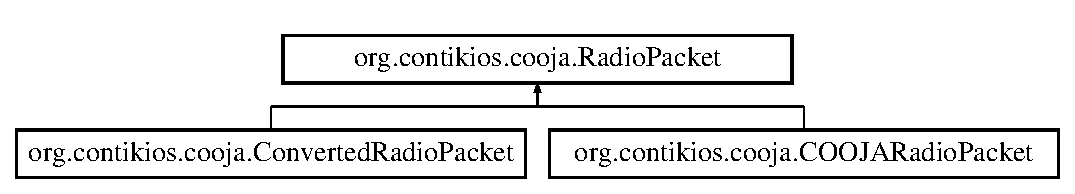
\includegraphics[height=2.000000cm]{interfaceorg_1_1contikios_1_1cooja_1_1RadioPacket}
\end{center}
\end{figure}
\subsection*{Public Member Functions}
\begin{DoxyCompactItemize}
\item 
byte\mbox{[}$\,$\mbox{]} \hyperlink{interfaceorg_1_1contikios_1_1cooja_1_1RadioPacket_aaff36d4c272ded32671f47ff68253415}{get\-Packet\-Data} ()
\end{DoxyCompactItemize}


\subsection{Detailed Description}
C\-O\-O\-J\-A's general radio packet. In order to support cross-\/level communication, all radios must support transmitting and receiving this packet. Radio implementations can additionally support custom data objects.

\begin{DoxySeeAlso}{See Also}
Custom\-Data\-Radio 

\hyperlink{classorg_1_1contikios_1_1cooja_1_1COOJARadioPacket}{C\-O\-O\-J\-A\-Radio\-Packet} 

\hyperlink{classorg_1_1contikios_1_1cooja_1_1ConvertedRadioPacket}{Converted\-Radio\-Packet} 
\end{DoxySeeAlso}
\begin{DoxyAuthor}{Author}
Fredrik Osterlind 
\end{DoxyAuthor}


\subsection{Member Function Documentation}
\hypertarget{interfaceorg_1_1contikios_1_1cooja_1_1RadioPacket_aaff36d4c272ded32671f47ff68253415}{\index{org\-::contikios\-::cooja\-::\-Radio\-Packet@{org\-::contikios\-::cooja\-::\-Radio\-Packet}!get\-Packet\-Data@{get\-Packet\-Data}}
\index{get\-Packet\-Data@{get\-Packet\-Data}!org::contikios::cooja::RadioPacket@{org\-::contikios\-::cooja\-::\-Radio\-Packet}}
\subsubsection[{get\-Packet\-Data}]{\setlength{\rightskip}{0pt plus 5cm}byte \mbox{[}$\,$\mbox{]} org.\-contikios.\-cooja.\-Radio\-Packet.\-get\-Packet\-Data (
\begin{DoxyParamCaption}
{}
\end{DoxyParamCaption}
)}}\label{interfaceorg_1_1contikios_1_1cooja_1_1RadioPacket_aaff36d4c272ded32671f47ff68253415}
\begin{DoxyReturn}{Returns}
Packet data 
\end{DoxyReturn}


Implemented in \hyperlink{classorg_1_1contikios_1_1cooja_1_1ConvertedRadioPacket_a2038c34dfd7e55daad454f8c34ddb33e}{org.\-contikios.\-cooja.\-Converted\-Radio\-Packet}, and \hyperlink{classorg_1_1contikios_1_1cooja_1_1COOJARadioPacket_a9322f1664dc941ebe8880a6530e526ff}{org.\-contikios.\-cooja.\-C\-O\-O\-J\-A\-Radio\-Packet}.



The documentation for this interface was generated from the following file\-:\begin{DoxyCompactItemize}
\item 
Radio\-Packet.\-java\end{DoxyCompactItemize}

\hypertarget{classorg_1_1contikios_1_1cooja_1_1SimEventCentral}{\section{org.\-contikios.\-cooja.\-Sim\-Event\-Central Class Reference}
\label{classorg_1_1contikios_1_1cooja_1_1SimEventCentral}\index{org.\-contikios.\-cooja.\-Sim\-Event\-Central@{org.\-contikios.\-cooja.\-Sim\-Event\-Central}}
}
\subsection*{Classes}
\begin{DoxyCompactItemize}
\item 
class {\bfseries Log\-Output\-Event}
\item 
interface \hyperlink{interfaceorg_1_1contikios_1_1cooja_1_1SimEventCentral_1_1LogOutputListener}{Log\-Output\-Listener}
\item 
interface \hyperlink{interfaceorg_1_1contikios_1_1cooja_1_1SimEventCentral_1_1MoteCountListener}{Mote\-Count\-Listener}
\end{DoxyCompactItemize}
\subsection*{Public Member Functions}
\begin{DoxyCompactItemize}
\item 
\hypertarget{classorg_1_1contikios_1_1cooja_1_1SimEventCentral_adc0a552d76979084295f4fc158e610dd}{{\bfseries Sim\-Event\-Central} (\hyperlink{classorg_1_1contikios_1_1cooja_1_1Simulation}{Simulation} simulation)}\label{classorg_1_1contikios_1_1cooja_1_1SimEventCentral_adc0a552d76979084295f4fc158e610dd}

\item 
\hypertarget{classorg_1_1contikios_1_1cooja_1_1SimEventCentral_af583b4642351137cafd5b0d862f9f8cf}{void {\bfseries add\-Mote\-Count\-Listener} (\hyperlink{interfaceorg_1_1contikios_1_1cooja_1_1SimEventCentral_1_1MoteCountListener}{Mote\-Count\-Listener} listener)}\label{classorg_1_1contikios_1_1cooja_1_1SimEventCentral_af583b4642351137cafd5b0d862f9f8cf}

\item 
\hypertarget{classorg_1_1contikios_1_1cooja_1_1SimEventCentral_a6059a5fc67695775cd420da127ee309a}{void {\bfseries remove\-Mote\-Count\-Listener} (\hyperlink{interfaceorg_1_1contikios_1_1cooja_1_1SimEventCentral_1_1MoteCountListener}{Mote\-Count\-Listener} listener)}\label{classorg_1_1contikios_1_1cooja_1_1SimEventCentral_a6059a5fc67695775cd420da127ee309a}

\item 
\hypertarget{classorg_1_1contikios_1_1cooja_1_1SimEventCentral_a8e59b7267843d4dafae21edab344b7b0}{void {\bfseries add\-Log\-Output\-Listener} (\hyperlink{interfaceorg_1_1contikios_1_1cooja_1_1SimEventCentral_1_1LogOutputListener}{Log\-Output\-Listener} listener)}\label{classorg_1_1contikios_1_1cooja_1_1SimEventCentral_a8e59b7267843d4dafae21edab344b7b0}

\item 
\hypertarget{classorg_1_1contikios_1_1cooja_1_1SimEventCentral_a76ee487df7496d3353d884e5cbc80aa0}{void {\bfseries remove\-Log\-Output\-Listener} (\hyperlink{interfaceorg_1_1contikios_1_1cooja_1_1SimEventCentral_1_1LogOutputListener}{Log\-Output\-Listener} listener)}\label{classorg_1_1contikios_1_1cooja_1_1SimEventCentral_a76ee487df7496d3353d884e5cbc80aa0}

\item 
\hypertarget{classorg_1_1contikios_1_1cooja_1_1SimEventCentral_ac172a82d13ff54e2a7b162e8074b578e}{Log\-Output\-Event\mbox{[}$\,$\mbox{]} {\bfseries get\-Log\-Output\-History} ()}\label{classorg_1_1contikios_1_1cooja_1_1SimEventCentral_ac172a82d13ff54e2a7b162e8074b578e}

\item 
\hypertarget{classorg_1_1contikios_1_1cooja_1_1SimEventCentral_a07f39e7030428b5a47c9e2bcfb60ba2a}{int {\bfseries get\-Log\-Output\-Buffer\-Size} ()}\label{classorg_1_1contikios_1_1cooja_1_1SimEventCentral_a07f39e7030428b5a47c9e2bcfb60ba2a}

\item 
\hypertarget{classorg_1_1contikios_1_1cooja_1_1SimEventCentral_a29a6217a9317db2328d414d31b7c149a}{void {\bfseries set\-Log\-Output\-Buffer\-Size} (int size)}\label{classorg_1_1contikios_1_1cooja_1_1SimEventCentral_a29a6217a9317db2328d414d31b7c149a}

\item 
\hypertarget{classorg_1_1contikios_1_1cooja_1_1SimEventCentral_af14b6324717c16b1dfd93463f4aeee31}{int {\bfseries get\-Log\-Output\-Observations\-Count} ()}\label{classorg_1_1contikios_1_1cooja_1_1SimEventCentral_af14b6324717c16b1dfd93463f4aeee31}

\item 
\hypertarget{classorg_1_1contikios_1_1cooja_1_1SimEventCentral_aac17a82fdfd32772827ee4e78ca6197d}{String {\bfseries to\-String} ()}\label{classorg_1_1contikios_1_1cooja_1_1SimEventCentral_aac17a82fdfd32772827ee4e78ca6197d}

\item 
\hypertarget{classorg_1_1contikios_1_1cooja_1_1SimEventCentral_a8f696c19dc950e97da932608e0976388}{Collection$<$ Element $>$ {\bfseries get\-Config\-X\-M\-L} ()}\label{classorg_1_1contikios_1_1cooja_1_1SimEventCentral_a8f696c19dc950e97da932608e0976388}

\item 
\hypertarget{classorg_1_1contikios_1_1cooja_1_1SimEventCentral_ad34fbe0521ba5def51c3713ae1bab5ff}{boolean {\bfseries set\-Config\-X\-M\-L} (\hyperlink{classorg_1_1contikios_1_1cooja_1_1Simulation}{Simulation} simulation, Collection$<$ Element $>$ config\-X\-M\-L, boolean vis\-Available)  throws Mote\-Type\-Creation\-Exception }\label{classorg_1_1contikios_1_1cooja_1_1SimEventCentral_ad34fbe0521ba5def51c3713ae1bab5ff}

\end{DoxyCompactItemize}


\subsection{Detailed Description}
\hyperlink{classorg_1_1contikios_1_1cooja_1_1Simulation}{Simulation} event central. Simplifies implementations of plugins that observe motes and mote interfaces by keeping track of added and removed motes. For a selected set of interfaces, the event central also maintains an event history.

\begin{DoxySeeAlso}{See Also}
Log\-Output\-Event 
\end{DoxySeeAlso}
\begin{DoxyAuthor}{Author}
Fredrik Osterlind 
\end{DoxyAuthor}


The documentation for this class was generated from the following file\-:\begin{DoxyCompactItemize}
\item 
Sim\-Event\-Central.\-java\end{DoxyCompactItemize}

\hypertarget{classorg_1_1contikios_1_1cooja_1_1Simulation}{\section{org.\-contikios.\-cooja.\-Simulation Class Reference}
\label{classorg_1_1contikios_1_1cooja_1_1Simulation}\index{org.\-contikios.\-cooja.\-Simulation@{org.\-contikios.\-cooja.\-Simulation}}
}
Inheritance diagram for org.\-contikios.\-cooja.\-Simulation\-:\begin{figure}[H]
\begin{center}
\leavevmode
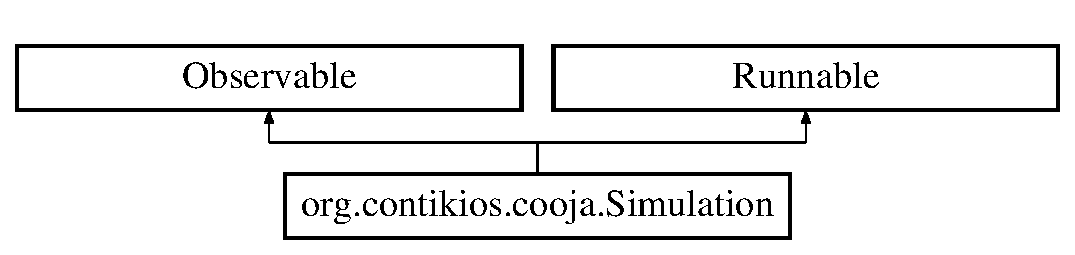
\includegraphics[height=2.000000cm]{classorg_1_1contikios_1_1cooja_1_1Simulation}
\end{center}
\end{figure}
\subsection*{Public Member Functions}
\begin{DoxyCompactItemize}
\item 
void \hyperlink{classorg_1_1contikios_1_1cooja_1_1Simulation_a0ef6f9dc924435b2eb386eb41950e803}{invoke\-Simulation\-Thread} (Runnable r)
\item 
void \hyperlink{classorg_1_1contikios_1_1cooja_1_1Simulation_a6c30336b3a1c4a2b4e17740537b0b830}{add\-Millisecond\-Observer} (Observer new\-Observer)
\item 
void \hyperlink{classorg_1_1contikios_1_1cooja_1_1Simulation_ab7e865094b023aa61fd427546d629aaa}{delete\-Millisecond\-Observer} (Observer observer)
\item 
boolean \hyperlink{classorg_1_1contikios_1_1cooja_1_1Simulation_a5b630fa3e827d876253cb8e8a3088577}{is\-Simulation\-Thread} ()
\item 
void \hyperlink{classorg_1_1contikios_1_1cooja_1_1Simulation_aba5d14753bd2be3fee0d1482fa1ec026}{schedule\-Event} (final \hyperlink{classorg_1_1contikios_1_1cooja_1_1TimeEvent}{Time\-Event} e, final long time)
\item 
\hypertarget{classorg_1_1contikios_1_1cooja_1_1Simulation_af1b7e348a4c69853a36d1b5271eb8b33}{void {\bfseries clear\-Events} ()}\label{classorg_1_1contikios_1_1cooja_1_1Simulation_af1b7e348a4c69853a36d1b5271eb8b33}

\item 
\hypertarget{classorg_1_1contikios_1_1cooja_1_1Simulation_a0b5be193cd0ff9afa7d0182d1402a86b}{void {\bfseries run} ()}\label{classorg_1_1contikios_1_1cooja_1_1Simulation_a0b5be193cd0ff9afa7d0182d1402a86b}

\item 
\hyperlink{classorg_1_1contikios_1_1cooja_1_1Simulation_a253e0212b6649aae4f15df59eac7082f}{Simulation} (\hyperlink{classorg_1_1contikios_1_1cooja_1_1Cooja}{Cooja} cooja)
\item 
void \hyperlink{classorg_1_1contikios_1_1cooja_1_1Simulation_a44a42bae3833b6e0ab14e386e29026e5}{start\-Simulation} ()
\item 
void \hyperlink{classorg_1_1contikios_1_1cooja_1_1Simulation_a81464528eba1e21ced1a88a39a9cf563}{stop\-Simulation} (boolean block)
\item 
void \hyperlink{classorg_1_1contikios_1_1cooja_1_1Simulation_aea5fa196be49ff54e8f9447aad24bde7}{stop\-Simulation} ()
\item 
void \hyperlink{classorg_1_1contikios_1_1cooja_1_1Simulation_a4d9db7c94ac1112e4f1b6b99c9a27154}{step\-Millisecond\-Simulation} ()
\item 
\hypertarget{classorg_1_1contikios_1_1cooja_1_1Simulation_adab9e988940ced2e52a9e0014a2aa2af}{\hyperlink{classorg_1_1contikios_1_1cooja_1_1Cooja}{Cooja} {\bfseries get\-Cooja} ()}\label{classorg_1_1contikios_1_1cooja_1_1Simulation_adab9e988940ced2e52a9e0014a2aa2af}

\item 
long \hyperlink{classorg_1_1contikios_1_1cooja_1_1Simulation_a310a51eb19707a9e847fec4b4b775926}{get\-Random\-Seed} ()
\item 
String \hyperlink{classorg_1_1contikios_1_1cooja_1_1Simulation_ace807bab2595c0bd0ca0340fdcc18f00}{get\-Random\-Seed\-String} ()
\item 
void \hyperlink{classorg_1_1contikios_1_1cooja_1_1Simulation_a722faaa06409286d004d9c27d9aa0bbc}{set\-Random\-Seed} (long random\-Seed)
\item 
void \hyperlink{classorg_1_1contikios_1_1cooja_1_1Simulation_a7397ff8b8cbd59f74f55f6675f878771}{set\-Random\-Seed\-Generated} (boolean generated)
\item 
boolean \hyperlink{classorg_1_1contikios_1_1cooja_1_1Simulation_acfed81b0086075e65c7bf0460d87aec2}{get\-Random\-Seed\-Generated} ()
\item 
\hypertarget{classorg_1_1contikios_1_1cooja_1_1Simulation_a9caa40fd1262afa7cabff6ea7d2a8e31}{Random {\bfseries get\-Random\-Generator} ()}\label{classorg_1_1contikios_1_1cooja_1_1Simulation_a9caa40fd1262afa7cabff6ea7d2a8e31}

\item 
long \hyperlink{classorg_1_1contikios_1_1cooja_1_1Simulation_a5d353adf641e2d4934c69401c9fed8c4}{get\-Delayed\-Mote\-Startup\-Time} ()
\item 
void \hyperlink{classorg_1_1contikios_1_1cooja_1_1Simulation_a04fda7fc1c736d53bd56590a692cc3fa}{set\-Delayed\-Mote\-Startup\-Time} (long max\-Mote\-Startup\-Delay)
\item 
\hypertarget{classorg_1_1contikios_1_1cooja_1_1Simulation_a308e19b3d0767003875ea1b4f66a796e}{\hyperlink{classorg_1_1contikios_1_1cooja_1_1SimEventCentral}{Sim\-Event\-Central} {\bfseries get\-Event\-Central} ()}\label{classorg_1_1contikios_1_1cooja_1_1Simulation_a308e19b3d0767003875ea1b4f66a796e}

\item 
Collection$<$ Element $>$ \hyperlink{classorg_1_1contikios_1_1cooja_1_1Simulation_ac612821b8df3d315a0af2982b167ea7f}{get\-Config\-X\-M\-L} ()
\item 
boolean \hyperlink{classorg_1_1contikios_1_1cooja_1_1Simulation_ae1b710dcc00cb8772117f248a2f64ac8}{set\-Config\-X\-M\-L} (Collection$<$ Element $>$ config\-X\-M\-L, boolean vis\-Available, Long manual\-Random\-Seed)  throws Exception 
\item 
void \hyperlink{classorg_1_1contikios_1_1cooja_1_1Simulation_aece7dddf684bed05eb5ef04d18bcd9df}{remove\-Mote} (final \hyperlink{interfaceorg_1_1contikios_1_1cooja_1_1Mote}{Mote} mote)
\item 
void \hyperlink{classorg_1_1contikios_1_1cooja_1_1Simulation_a1496782314ae0cb2a4318e573cf95364}{removed} ()
\item 
void \hyperlink{classorg_1_1contikios_1_1cooja_1_1Simulation_af5707101a76c8cb2ca3a411d52f5a973}{add\-Mote} (final \hyperlink{interfaceorg_1_1contikios_1_1cooja_1_1Mote}{Mote} mote)
\item 
\hyperlink{interfaceorg_1_1contikios_1_1cooja_1_1Mote}{Mote} \hyperlink{classorg_1_1contikios_1_1cooja_1_1Simulation_aa862d8ad1e7d37cb95a8a63372ba443b}{get\-Mote} (int pos)
\item 
\hyperlink{interfaceorg_1_1contikios_1_1cooja_1_1Mote}{Mote} \hyperlink{classorg_1_1contikios_1_1cooja_1_1Simulation_a4afc60021ede033bd050eb1b80093b71}{get\-Mote\-With\-I\-D} (int id)
\item 
\hyperlink{interfaceorg_1_1contikios_1_1cooja_1_1Mote}{Mote} \hyperlink{classorg_1_1contikios_1_1cooja_1_1Simulation_aedff300078e00e6cb3d1b9b0f06c7461}{get\-Mote\-With\-I\-D\-Uninit} (int id)
\item 
int \hyperlink{classorg_1_1contikios_1_1cooja_1_1Simulation_aa056449b5fb1346d843c9de2f5a3baea}{get\-Motes\-Count} ()
\item 
\hyperlink{interfaceorg_1_1contikios_1_1cooja_1_1Mote}{Mote}\mbox{[}$\,$\mbox{]} \hyperlink{classorg_1_1contikios_1_1cooja_1_1Simulation_a7594b1f093455b52ad9bab91ad39eebb}{get\-Motes} ()
\item 
\hyperlink{interfaceorg_1_1contikios_1_1cooja_1_1Mote}{Mote}\mbox{[}$\,$\mbox{]} \hyperlink{classorg_1_1contikios_1_1cooja_1_1Simulation_af9935db82c2e37bf2171d0a972e65281}{get\-Motes\-Uninit} ()
\item 
\hyperlink{interfaceorg_1_1contikios_1_1cooja_1_1MoteType}{Mote\-Type}\mbox{[}$\,$\mbox{]} \hyperlink{classorg_1_1contikios_1_1cooja_1_1Simulation_a9ce6f6674fb675e655becc5af3e082dd}{get\-Mote\-Types} ()
\item 
\hyperlink{interfaceorg_1_1contikios_1_1cooja_1_1MoteType}{Mote\-Type} \hyperlink{classorg_1_1contikios_1_1cooja_1_1Simulation_a6a2def16017d97357c70b65d76b8a561}{get\-Mote\-Type} (String identifier)
\item 
void \hyperlink{classorg_1_1contikios_1_1cooja_1_1Simulation_aafe354c8d241a7d02320168947dc0cd4}{add\-Mote\-Type} (\hyperlink{interfaceorg_1_1contikios_1_1cooja_1_1MoteType}{Mote\-Type} new\-Mote\-Type)
\item 
void \hyperlink{classorg_1_1contikios_1_1cooja_1_1Simulation_ac8add8afcbeb281aa72b35813a9e998e}{remove\-Mote\-Type} (\hyperlink{interfaceorg_1_1contikios_1_1cooja_1_1MoteType}{Mote\-Type} type)
\item 
void \hyperlink{classorg_1_1contikios_1_1cooja_1_1Simulation_a1eebb975bc564108f149006e53865a41}{set\-Speed\-Limit} (final Double new\-Speed\-Limit)
\item 
Double \hyperlink{classorg_1_1contikios_1_1cooja_1_1Simulation_a49ca7c43f77d7842b0d7cf8bc7a9d59b}{get\-Speed\-Limit} ()
\item 
void \hyperlink{classorg_1_1contikios_1_1cooja_1_1Simulation_a38ea8498edad5fe60da724f940019e34}{set\-Simulation\-Time} (long simulation\-Time)
\item 
long \hyperlink{classorg_1_1contikios_1_1cooja_1_1Simulation_a62bd4b8997b5debaab80378847802a03}{get\-Simulation\-Time} ()
\item 
long \hyperlink{classorg_1_1contikios_1_1cooja_1_1Simulation_aed2aa6f9d4f3399db5a165ecec79d377}{get\-Simulation\-Time\-Millis} ()
\item 
void \hyperlink{classorg_1_1contikios_1_1cooja_1_1Simulation_ae3bc11e84ccd6ec80972ae3721cce982}{set\-Radio\-Medium} (\hyperlink{classorg_1_1contikios_1_1cooja_1_1RadioMedium}{Radio\-Medium} radio\-Medium)
\item 
\hyperlink{classorg_1_1contikios_1_1cooja_1_1RadioMedium}{Radio\-Medium} \hyperlink{classorg_1_1contikios_1_1cooja_1_1Simulation_a6698a9b238ebf1bf163935e49dea7ba2}{get\-Radio\-Medium} ()
\item 
boolean \hyperlink{classorg_1_1contikios_1_1cooja_1_1Simulation_a1298fc918e33caa7b0a00b716046ea20}{is\-Running} ()
\item 
boolean \hyperlink{classorg_1_1contikios_1_1cooja_1_1Simulation_a56e2232b682eb1b22d9763e7a668b6d8}{is\-Runnable} ()
\item 
String \hyperlink{classorg_1_1contikios_1_1cooja_1_1Simulation_a42c89234ae8bd779d1b13713a1d155d1}{get\-Title} ()
\item 
void \hyperlink{classorg_1_1contikios_1_1cooja_1_1Simulation_a48185c6495c9c77c02a5db194ab11ebb}{set\-Title} (String title)
\end{DoxyCompactItemize}
\subsection*{Static Public Attributes}
\begin{DoxyCompactItemize}
\item 
\hypertarget{classorg_1_1contikios_1_1cooja_1_1Simulation_aa75fc5b61129ec8a4333296d04faeb1e}{static final long {\bfseries M\-I\-C\-R\-O\-S\-E\-C\-O\-N\-D} = 1\-L}\label{classorg_1_1contikios_1_1cooja_1_1Simulation_aa75fc5b61129ec8a4333296d04faeb1e}

\item 
\hypertarget{classorg_1_1contikios_1_1cooja_1_1Simulation_a357ccb425bd7d749cf41f0cbbde40748}{static final long {\bfseries M\-I\-L\-L\-I\-S\-E\-C\-O\-N\-D} = 1000$\ast$M\-I\-C\-R\-O\-S\-E\-C\-O\-N\-D}\label{classorg_1_1contikios_1_1cooja_1_1Simulation_a357ccb425bd7d749cf41f0cbbde40748}

\end{DoxyCompactItemize}


\subsection{Detailed Description}
A simulation consists of a number of motes and mote types.

A simulation is observable\-: changed simulation state, added or deleted motes etc are observed. To track mote changes, observe the mote (interfaces) itself.

\begin{DoxyAuthor}{Author}
Fredrik Osterlind 
\end{DoxyAuthor}


\subsection{Constructor \& Destructor Documentation}
\hypertarget{classorg_1_1contikios_1_1cooja_1_1Simulation_a253e0212b6649aae4f15df59eac7082f}{\index{org\-::contikios\-::cooja\-::\-Simulation@{org\-::contikios\-::cooja\-::\-Simulation}!Simulation@{Simulation}}
\index{Simulation@{Simulation}!org::contikios::cooja::Simulation@{org\-::contikios\-::cooja\-::\-Simulation}}
\subsubsection[{Simulation}]{\setlength{\rightskip}{0pt plus 5cm}org.\-contikios.\-cooja.\-Simulation.\-Simulation (
\begin{DoxyParamCaption}
\item[{{\bf Cooja}}]{cooja}
\end{DoxyParamCaption}
)\hspace{0.3cm}{\ttfamily [inline]}}}\label{classorg_1_1contikios_1_1cooja_1_1Simulation_a253e0212b6649aae4f15df59eac7082f}
Creates a new simulation 

\subsection{Member Function Documentation}
\hypertarget{classorg_1_1contikios_1_1cooja_1_1Simulation_a6c30336b3a1c4a2b4e17740537b0b830}{\index{org\-::contikios\-::cooja\-::\-Simulation@{org\-::contikios\-::cooja\-::\-Simulation}!add\-Millisecond\-Observer@{add\-Millisecond\-Observer}}
\index{add\-Millisecond\-Observer@{add\-Millisecond\-Observer}!org::contikios::cooja::Simulation@{org\-::contikios\-::cooja\-::\-Simulation}}
\subsubsection[{add\-Millisecond\-Observer}]{\setlength{\rightskip}{0pt plus 5cm}void org.\-contikios.\-cooja.\-Simulation.\-add\-Millisecond\-Observer (
\begin{DoxyParamCaption}
\item[{Observer}]{new\-Observer}
\end{DoxyParamCaption}
)\hspace{0.3cm}{\ttfamily [inline]}}}\label{classorg_1_1contikios_1_1cooja_1_1Simulation_a6c30336b3a1c4a2b4e17740537b0b830}
Add millisecond observer. This observer is notified once every simulated millisecond.

\begin{DoxySeeAlso}{See Also}
\hyperlink{classorg_1_1contikios_1_1cooja_1_1Simulation_ab7e865094b023aa61fd427546d629aaa}{delete\-Millisecond\-Observer(\-Observer)} 
\end{DoxySeeAlso}

\begin{DoxyParams}{Parameters}
{\em new\-Observer} & Observer \\
\hline
\end{DoxyParams}
\hypertarget{classorg_1_1contikios_1_1cooja_1_1Simulation_af5707101a76c8cb2ca3a411d52f5a973}{\index{org\-::contikios\-::cooja\-::\-Simulation@{org\-::contikios\-::cooja\-::\-Simulation}!add\-Mote@{add\-Mote}}
\index{add\-Mote@{add\-Mote}!org::contikios::cooja::Simulation@{org\-::contikios\-::cooja\-::\-Simulation}}
\subsubsection[{add\-Mote}]{\setlength{\rightskip}{0pt plus 5cm}void org.\-contikios.\-cooja.\-Simulation.\-add\-Mote (
\begin{DoxyParamCaption}
\item[{final {\bf Mote}}]{mote}
\end{DoxyParamCaption}
)\hspace{0.3cm}{\ttfamily [inline]}}}\label{classorg_1_1contikios_1_1cooja_1_1Simulation_af5707101a76c8cb2ca3a411d52f5a973}
Adds a mote to this simulation


\begin{DoxyParams}{Parameters}
{\em mote} & \hyperlink{interfaceorg_1_1contikios_1_1cooja_1_1Mote}{Mote} to add \\
\hline
\end{DoxyParams}
\hypertarget{classorg_1_1contikios_1_1cooja_1_1Simulation_aafe354c8d241a7d02320168947dc0cd4}{\index{org\-::contikios\-::cooja\-::\-Simulation@{org\-::contikios\-::cooja\-::\-Simulation}!add\-Mote\-Type@{add\-Mote\-Type}}
\index{add\-Mote\-Type@{add\-Mote\-Type}!org::contikios::cooja::Simulation@{org\-::contikios\-::cooja\-::\-Simulation}}
\subsubsection[{add\-Mote\-Type}]{\setlength{\rightskip}{0pt plus 5cm}void org.\-contikios.\-cooja.\-Simulation.\-add\-Mote\-Type (
\begin{DoxyParamCaption}
\item[{{\bf Mote\-Type}}]{new\-Mote\-Type}
\end{DoxyParamCaption}
)\hspace{0.3cm}{\ttfamily [inline]}}}\label{classorg_1_1contikios_1_1cooja_1_1Simulation_aafe354c8d241a7d02320168947dc0cd4}
Adds given mote type to simulation.


\begin{DoxyParams}{Parameters}
{\em new\-Mote\-Type} & \hyperlink{interfaceorg_1_1contikios_1_1cooja_1_1Mote}{Mote} type \\
\hline
\end{DoxyParams}
\hypertarget{classorg_1_1contikios_1_1cooja_1_1Simulation_ab7e865094b023aa61fd427546d629aaa}{\index{org\-::contikios\-::cooja\-::\-Simulation@{org\-::contikios\-::cooja\-::\-Simulation}!delete\-Millisecond\-Observer@{delete\-Millisecond\-Observer}}
\index{delete\-Millisecond\-Observer@{delete\-Millisecond\-Observer}!org::contikios::cooja::Simulation@{org\-::contikios\-::cooja\-::\-Simulation}}
\subsubsection[{delete\-Millisecond\-Observer}]{\setlength{\rightskip}{0pt plus 5cm}void org.\-contikios.\-cooja.\-Simulation.\-delete\-Millisecond\-Observer (
\begin{DoxyParamCaption}
\item[{Observer}]{observer}
\end{DoxyParamCaption}
)\hspace{0.3cm}{\ttfamily [inline]}}}\label{classorg_1_1contikios_1_1cooja_1_1Simulation_ab7e865094b023aa61fd427546d629aaa}
Delete millisecond observer.

\begin{DoxySeeAlso}{See Also}
\hyperlink{classorg_1_1contikios_1_1cooja_1_1Simulation_a6c30336b3a1c4a2b4e17740537b0b830}{add\-Millisecond\-Observer(\-Observer)} 
\end{DoxySeeAlso}

\begin{DoxyParams}{Parameters}
{\em observer} & Observer to delete \\
\hline
\end{DoxyParams}
\hypertarget{classorg_1_1contikios_1_1cooja_1_1Simulation_ac612821b8df3d315a0af2982b167ea7f}{\index{org\-::contikios\-::cooja\-::\-Simulation@{org\-::contikios\-::cooja\-::\-Simulation}!get\-Config\-X\-M\-L@{get\-Config\-X\-M\-L}}
\index{get\-Config\-X\-M\-L@{get\-Config\-X\-M\-L}!org::contikios::cooja::Simulation@{org\-::contikios\-::cooja\-::\-Simulation}}
\subsubsection[{get\-Config\-X\-M\-L}]{\setlength{\rightskip}{0pt plus 5cm}Collection$<$Element$>$ org.\-contikios.\-cooja.\-Simulation.\-get\-Config\-X\-M\-L (
\begin{DoxyParamCaption}
{}
\end{DoxyParamCaption}
)\hspace{0.3cm}{\ttfamily [inline]}}}\label{classorg_1_1contikios_1_1cooja_1_1Simulation_ac612821b8df3d315a0af2982b167ea7f}
Returns the current simulation config represented by X\-M\-L elements. This config also includes the current radio medium, all mote types and motes.

\begin{DoxyReturn}{Returns}
Current simulation config 
\end{DoxyReturn}
\hypertarget{classorg_1_1contikios_1_1cooja_1_1Simulation_a5d353adf641e2d4934c69401c9fed8c4}{\index{org\-::contikios\-::cooja\-::\-Simulation@{org\-::contikios\-::cooja\-::\-Simulation}!get\-Delayed\-Mote\-Startup\-Time@{get\-Delayed\-Mote\-Startup\-Time}}
\index{get\-Delayed\-Mote\-Startup\-Time@{get\-Delayed\-Mote\-Startup\-Time}!org::contikios::cooja::Simulation@{org\-::contikios\-::cooja\-::\-Simulation}}
\subsubsection[{get\-Delayed\-Mote\-Startup\-Time}]{\setlength{\rightskip}{0pt plus 5cm}long org.\-contikios.\-cooja.\-Simulation.\-get\-Delayed\-Mote\-Startup\-Time (
\begin{DoxyParamCaption}
{}
\end{DoxyParamCaption}
)\hspace{0.3cm}{\ttfamily [inline]}}}\label{classorg_1_1contikios_1_1cooja_1_1Simulation_a5d353adf641e2d4934c69401c9fed8c4}
\begin{DoxyReturn}{Returns}
Maximum mote startup delay 
\end{DoxyReturn}
\hypertarget{classorg_1_1contikios_1_1cooja_1_1Simulation_aa862d8ad1e7d37cb95a8a63372ba443b}{\index{org\-::contikios\-::cooja\-::\-Simulation@{org\-::contikios\-::cooja\-::\-Simulation}!get\-Mote@{get\-Mote}}
\index{get\-Mote@{get\-Mote}!org::contikios::cooja::Simulation@{org\-::contikios\-::cooja\-::\-Simulation}}
\subsubsection[{get\-Mote}]{\setlength{\rightskip}{0pt plus 5cm}{\bf Mote} org.\-contikios.\-cooja.\-Simulation.\-get\-Mote (
\begin{DoxyParamCaption}
\item[{int}]{pos}
\end{DoxyParamCaption}
)\hspace{0.3cm}{\ttfamily [inline]}}}\label{classorg_1_1contikios_1_1cooja_1_1Simulation_aa862d8ad1e7d37cb95a8a63372ba443b}
Returns simulation mote at given list position.


\begin{DoxyParams}{Parameters}
{\em pos} & Internal list position of mote \\
\hline
\end{DoxyParams}
\begin{DoxyReturn}{Returns}
\hyperlink{interfaceorg_1_1contikios_1_1cooja_1_1Mote}{Mote} 
\end{DoxyReturn}
\begin{DoxySeeAlso}{See Also}
\hyperlink{classorg_1_1contikios_1_1cooja_1_1Simulation_aa056449b5fb1346d843c9de2f5a3baea}{get\-Motes\-Count()} 

\hyperlink{classorg_1_1contikios_1_1cooja_1_1Simulation_a4afc60021ede033bd050eb1b80093b71}{get\-Mote\-With\-I\-D(int)} 
\end{DoxySeeAlso}
\hypertarget{classorg_1_1contikios_1_1cooja_1_1Simulation_a7594b1f093455b52ad9bab91ad39eebb}{\index{org\-::contikios\-::cooja\-::\-Simulation@{org\-::contikios\-::cooja\-::\-Simulation}!get\-Motes@{get\-Motes}}
\index{get\-Motes@{get\-Motes}!org::contikios::cooja::Simulation@{org\-::contikios\-::cooja\-::\-Simulation}}
\subsubsection[{get\-Motes}]{\setlength{\rightskip}{0pt plus 5cm}{\bf Mote} \mbox{[}$\,$\mbox{]} org.\-contikios.\-cooja.\-Simulation.\-get\-Motes (
\begin{DoxyParamCaption}
{}
\end{DoxyParamCaption}
)\hspace{0.3cm}{\ttfamily [inline]}}}\label{classorg_1_1contikios_1_1cooja_1_1Simulation_a7594b1f093455b52ad9bab91ad39eebb}
Returns all motes in this simulation.

\begin{DoxyReturn}{Returns}
Motes 
\end{DoxyReturn}
\hypertarget{classorg_1_1contikios_1_1cooja_1_1Simulation_aa056449b5fb1346d843c9de2f5a3baea}{\index{org\-::contikios\-::cooja\-::\-Simulation@{org\-::contikios\-::cooja\-::\-Simulation}!get\-Motes\-Count@{get\-Motes\-Count}}
\index{get\-Motes\-Count@{get\-Motes\-Count}!org::contikios::cooja::Simulation@{org\-::contikios\-::cooja\-::\-Simulation}}
\subsubsection[{get\-Motes\-Count}]{\setlength{\rightskip}{0pt plus 5cm}int org.\-contikios.\-cooja.\-Simulation.\-get\-Motes\-Count (
\begin{DoxyParamCaption}
{}
\end{DoxyParamCaption}
)\hspace{0.3cm}{\ttfamily [inline]}}}\label{classorg_1_1contikios_1_1cooja_1_1Simulation_aa056449b5fb1346d843c9de2f5a3baea}
Returns number of motes in this simulation.

\begin{DoxyReturn}{Returns}
Number of motes 
\end{DoxyReturn}
\hypertarget{classorg_1_1contikios_1_1cooja_1_1Simulation_af9935db82c2e37bf2171d0a972e65281}{\index{org\-::contikios\-::cooja\-::\-Simulation@{org\-::contikios\-::cooja\-::\-Simulation}!get\-Motes\-Uninit@{get\-Motes\-Uninit}}
\index{get\-Motes\-Uninit@{get\-Motes\-Uninit}!org::contikios::cooja::Simulation@{org\-::contikios\-::cooja\-::\-Simulation}}
\subsubsection[{get\-Motes\-Uninit}]{\setlength{\rightskip}{0pt plus 5cm}{\bf Mote} \mbox{[}$\,$\mbox{]} org.\-contikios.\-cooja.\-Simulation.\-get\-Motes\-Uninit (
\begin{DoxyParamCaption}
{}
\end{DoxyParamCaption}
)\hspace{0.3cm}{\ttfamily [inline]}}}\label{classorg_1_1contikios_1_1cooja_1_1Simulation_af9935db82c2e37bf2171d0a972e65281}
Returns uninitialised motes

\begin{DoxyReturn}{Returns}
Motes 
\end{DoxyReturn}
\hypertarget{classorg_1_1contikios_1_1cooja_1_1Simulation_a6a2def16017d97357c70b65d76b8a561}{\index{org\-::contikios\-::cooja\-::\-Simulation@{org\-::contikios\-::cooja\-::\-Simulation}!get\-Mote\-Type@{get\-Mote\-Type}}
\index{get\-Mote\-Type@{get\-Mote\-Type}!org::contikios::cooja::Simulation@{org\-::contikios\-::cooja\-::\-Simulation}}
\subsubsection[{get\-Mote\-Type}]{\setlength{\rightskip}{0pt plus 5cm}{\bf Mote\-Type} org.\-contikios.\-cooja.\-Simulation.\-get\-Mote\-Type (
\begin{DoxyParamCaption}
\item[{String}]{identifier}
\end{DoxyParamCaption}
)\hspace{0.3cm}{\ttfamily [inline]}}}\label{classorg_1_1contikios_1_1cooja_1_1Simulation_a6a2def16017d97357c70b65d76b8a561}
Returns mote type with given identifier.


\begin{DoxyParams}{Parameters}
{\em identifier} & \hyperlink{interfaceorg_1_1contikios_1_1cooja_1_1Mote}{Mote} type identifier \\
\hline
\end{DoxyParams}
\begin{DoxyReturn}{Returns}
\hyperlink{interfaceorg_1_1contikios_1_1cooja_1_1Mote}{Mote} type or null if not found 
\end{DoxyReturn}
\hypertarget{classorg_1_1contikios_1_1cooja_1_1Simulation_a9ce6f6674fb675e655becc5af3e082dd}{\index{org\-::contikios\-::cooja\-::\-Simulation@{org\-::contikios\-::cooja\-::\-Simulation}!get\-Mote\-Types@{get\-Mote\-Types}}
\index{get\-Mote\-Types@{get\-Mote\-Types}!org::contikios::cooja::Simulation@{org\-::contikios\-::cooja\-::\-Simulation}}
\subsubsection[{get\-Mote\-Types}]{\setlength{\rightskip}{0pt plus 5cm}{\bf Mote\-Type} \mbox{[}$\,$\mbox{]} org.\-contikios.\-cooja.\-Simulation.\-get\-Mote\-Types (
\begin{DoxyParamCaption}
{}
\end{DoxyParamCaption}
)\hspace{0.3cm}{\ttfamily [inline]}}}\label{classorg_1_1contikios_1_1cooja_1_1Simulation_a9ce6f6674fb675e655becc5af3e082dd}
Returns all mote types in simulation.

\begin{DoxyReturn}{Returns}
All mote types 
\end{DoxyReturn}
\hypertarget{classorg_1_1contikios_1_1cooja_1_1Simulation_a4afc60021ede033bd050eb1b80093b71}{\index{org\-::contikios\-::cooja\-::\-Simulation@{org\-::contikios\-::cooja\-::\-Simulation}!get\-Mote\-With\-I\-D@{get\-Mote\-With\-I\-D}}
\index{get\-Mote\-With\-I\-D@{get\-Mote\-With\-I\-D}!org::contikios::cooja::Simulation@{org\-::contikios\-::cooja\-::\-Simulation}}
\subsubsection[{get\-Mote\-With\-I\-D}]{\setlength{\rightskip}{0pt plus 5cm}{\bf Mote} org.\-contikios.\-cooja.\-Simulation.\-get\-Mote\-With\-I\-D (
\begin{DoxyParamCaption}
\item[{int}]{id}
\end{DoxyParamCaption}
)\hspace{0.3cm}{\ttfamily [inline]}}}\label{classorg_1_1contikios_1_1cooja_1_1Simulation_a4afc60021ede033bd050eb1b80093b71}
Returns simulation with with given I\-D.


\begin{DoxyParams}{Parameters}
{\em id} & I\-D \\
\hline
\end{DoxyParams}
\begin{DoxyReturn}{Returns}
\hyperlink{interfaceorg_1_1contikios_1_1cooja_1_1Mote}{Mote} or null 
\end{DoxyReturn}
\begin{DoxySeeAlso}{See Also}
\hyperlink{interfaceorg_1_1contikios_1_1cooja_1_1Mote_ace9d66ac50f3dba7ae725a16a8172aa6}{Mote\-::get\-I\-D()} 
\end{DoxySeeAlso}
\hypertarget{classorg_1_1contikios_1_1cooja_1_1Simulation_aedff300078e00e6cb3d1b9b0f06c7461}{\index{org\-::contikios\-::cooja\-::\-Simulation@{org\-::contikios\-::cooja\-::\-Simulation}!get\-Mote\-With\-I\-D\-Uninit@{get\-Mote\-With\-I\-D\-Uninit}}
\index{get\-Mote\-With\-I\-D\-Uninit@{get\-Mote\-With\-I\-D\-Uninit}!org::contikios::cooja::Simulation@{org\-::contikios\-::cooja\-::\-Simulation}}
\subsubsection[{get\-Mote\-With\-I\-D\-Uninit}]{\setlength{\rightskip}{0pt plus 5cm}{\bf Mote} org.\-contikios.\-cooja.\-Simulation.\-get\-Mote\-With\-I\-D\-Uninit (
\begin{DoxyParamCaption}
\item[{int}]{id}
\end{DoxyParamCaption}
)\hspace{0.3cm}{\ttfamily [inline]}}}\label{classorg_1_1contikios_1_1cooja_1_1Simulation_aedff300078e00e6cb3d1b9b0f06c7461}
Returns uninitialised simulation mote with with given I\-D.


\begin{DoxyParams}{Parameters}
{\em id} & I\-D \\
\hline
\end{DoxyParams}
\begin{DoxyReturn}{Returns}
\hyperlink{interfaceorg_1_1contikios_1_1cooja_1_1Mote}{Mote} or null 
\end{DoxyReturn}
\begin{DoxySeeAlso}{See Also}
\hyperlink{interfaceorg_1_1contikios_1_1cooja_1_1Mote_ace9d66ac50f3dba7ae725a16a8172aa6}{Mote\-::get\-I\-D()} 
\end{DoxySeeAlso}
\hypertarget{classorg_1_1contikios_1_1cooja_1_1Simulation_a6698a9b238ebf1bf163935e49dea7ba2}{\index{org\-::contikios\-::cooja\-::\-Simulation@{org\-::contikios\-::cooja\-::\-Simulation}!get\-Radio\-Medium@{get\-Radio\-Medium}}
\index{get\-Radio\-Medium@{get\-Radio\-Medium}!org::contikios::cooja::Simulation@{org\-::contikios\-::cooja\-::\-Simulation}}
\subsubsection[{get\-Radio\-Medium}]{\setlength{\rightskip}{0pt plus 5cm}{\bf Radio\-Medium} org.\-contikios.\-cooja.\-Simulation.\-get\-Radio\-Medium (
\begin{DoxyParamCaption}
{}
\end{DoxyParamCaption}
)\hspace{0.3cm}{\ttfamily [inline]}}}\label{classorg_1_1contikios_1_1cooja_1_1Simulation_a6698a9b238ebf1bf163935e49dea7ba2}
Get currently used radio medium.

\begin{DoxyReturn}{Returns}
Currently used radio medium 
\end{DoxyReturn}
\hypertarget{classorg_1_1contikios_1_1cooja_1_1Simulation_a310a51eb19707a9e847fec4b4b775926}{\index{org\-::contikios\-::cooja\-::\-Simulation@{org\-::contikios\-::cooja\-::\-Simulation}!get\-Random\-Seed@{get\-Random\-Seed}}
\index{get\-Random\-Seed@{get\-Random\-Seed}!org::contikios::cooja::Simulation@{org\-::contikios\-::cooja\-::\-Simulation}}
\subsubsection[{get\-Random\-Seed}]{\setlength{\rightskip}{0pt plus 5cm}long org.\-contikios.\-cooja.\-Simulation.\-get\-Random\-Seed (
\begin{DoxyParamCaption}
{}
\end{DoxyParamCaption}
)\hspace{0.3cm}{\ttfamily [inline]}}}\label{classorg_1_1contikios_1_1cooja_1_1Simulation_a310a51eb19707a9e847fec4b4b775926}
\begin{DoxyReturn}{Returns}
Random seed 
\end{DoxyReturn}
\hypertarget{classorg_1_1contikios_1_1cooja_1_1Simulation_acfed81b0086075e65c7bf0460d87aec2}{\index{org\-::contikios\-::cooja\-::\-Simulation@{org\-::contikios\-::cooja\-::\-Simulation}!get\-Random\-Seed\-Generated@{get\-Random\-Seed\-Generated}}
\index{get\-Random\-Seed\-Generated@{get\-Random\-Seed\-Generated}!org::contikios::cooja::Simulation@{org\-::contikios\-::cooja\-::\-Simulation}}
\subsubsection[{get\-Random\-Seed\-Generated}]{\setlength{\rightskip}{0pt plus 5cm}boolean org.\-contikios.\-cooja.\-Simulation.\-get\-Random\-Seed\-Generated (
\begin{DoxyParamCaption}
{}
\end{DoxyParamCaption}
)\hspace{0.3cm}{\ttfamily [inline]}}}\label{classorg_1_1contikios_1_1cooja_1_1Simulation_acfed81b0086075e65c7bf0460d87aec2}
\begin{DoxyReturn}{Returns}
Autogenerated random seed at simulation load 
\end{DoxyReturn}
\hypertarget{classorg_1_1contikios_1_1cooja_1_1Simulation_ace807bab2595c0bd0ca0340fdcc18f00}{\index{org\-::contikios\-::cooja\-::\-Simulation@{org\-::contikios\-::cooja\-::\-Simulation}!get\-Random\-Seed\-String@{get\-Random\-Seed\-String}}
\index{get\-Random\-Seed\-String@{get\-Random\-Seed\-String}!org::contikios::cooja::Simulation@{org\-::contikios\-::cooja\-::\-Simulation}}
\subsubsection[{get\-Random\-Seed\-String}]{\setlength{\rightskip}{0pt plus 5cm}String org.\-contikios.\-cooja.\-Simulation.\-get\-Random\-Seed\-String (
\begin{DoxyParamCaption}
{}
\end{DoxyParamCaption}
)\hspace{0.3cm}{\ttfamily [inline]}}}\label{classorg_1_1contikios_1_1cooja_1_1Simulation_ace807bab2595c0bd0ca0340fdcc18f00}
\begin{DoxyReturn}{Returns}
Random seed (converted to a string) 
\end{DoxyReturn}
\hypertarget{classorg_1_1contikios_1_1cooja_1_1Simulation_a62bd4b8997b5debaab80378847802a03}{\index{org\-::contikios\-::cooja\-::\-Simulation@{org\-::contikios\-::cooja\-::\-Simulation}!get\-Simulation\-Time@{get\-Simulation\-Time}}
\index{get\-Simulation\-Time@{get\-Simulation\-Time}!org::contikios::cooja::Simulation@{org\-::contikios\-::cooja\-::\-Simulation}}
\subsubsection[{get\-Simulation\-Time}]{\setlength{\rightskip}{0pt plus 5cm}long org.\-contikios.\-cooja.\-Simulation.\-get\-Simulation\-Time (
\begin{DoxyParamCaption}
{}
\end{DoxyParamCaption}
)\hspace{0.3cm}{\ttfamily [inline]}}}\label{classorg_1_1contikios_1_1cooja_1_1Simulation_a62bd4b8997b5debaab80378847802a03}
Returns current simulation time.

\begin{DoxyReturn}{Returns}
\hyperlink{classorg_1_1contikios_1_1cooja_1_1Simulation}{Simulation} time (microseconds) 
\end{DoxyReturn}
\hypertarget{classorg_1_1contikios_1_1cooja_1_1Simulation_aed2aa6f9d4f3399db5a165ecec79d377}{\index{org\-::contikios\-::cooja\-::\-Simulation@{org\-::contikios\-::cooja\-::\-Simulation}!get\-Simulation\-Time\-Millis@{get\-Simulation\-Time\-Millis}}
\index{get\-Simulation\-Time\-Millis@{get\-Simulation\-Time\-Millis}!org::contikios::cooja::Simulation@{org\-::contikios\-::cooja\-::\-Simulation}}
\subsubsection[{get\-Simulation\-Time\-Millis}]{\setlength{\rightskip}{0pt plus 5cm}long org.\-contikios.\-cooja.\-Simulation.\-get\-Simulation\-Time\-Millis (
\begin{DoxyParamCaption}
{}
\end{DoxyParamCaption}
)\hspace{0.3cm}{\ttfamily [inline]}}}\label{classorg_1_1contikios_1_1cooja_1_1Simulation_aed2aa6f9d4f3399db5a165ecec79d377}
Returns current simulation time rounded to milliseconds.

\begin{DoxySeeAlso}{See Also}
\hyperlink{classorg_1_1contikios_1_1cooja_1_1Simulation_a62bd4b8997b5debaab80378847802a03}{get\-Simulation\-Time()} 
\end{DoxySeeAlso}
\begin{DoxyReturn}{Returns}
Time rounded to milliseconds 
\end{DoxyReturn}
\hypertarget{classorg_1_1contikios_1_1cooja_1_1Simulation_a49ca7c43f77d7842b0d7cf8bc7a9d59b}{\index{org\-::contikios\-::cooja\-::\-Simulation@{org\-::contikios\-::cooja\-::\-Simulation}!get\-Speed\-Limit@{get\-Speed\-Limit}}
\index{get\-Speed\-Limit@{get\-Speed\-Limit}!org::contikios::cooja::Simulation@{org\-::contikios\-::cooja\-::\-Simulation}}
\subsubsection[{get\-Speed\-Limit}]{\setlength{\rightskip}{0pt plus 5cm}Double org.\-contikios.\-cooja.\-Simulation.\-get\-Speed\-Limit (
\begin{DoxyParamCaption}
{}
\end{DoxyParamCaption}
)\hspace{0.3cm}{\ttfamily [inline]}}}\label{classorg_1_1contikios_1_1cooja_1_1Simulation_a49ca7c43f77d7842b0d7cf8bc7a9d59b}
\begin{DoxyReturn}{Returns}
Max simulation speed ratio. Returns null if no limit. 
\end{DoxyReturn}
\hypertarget{classorg_1_1contikios_1_1cooja_1_1Simulation_a42c89234ae8bd779d1b13713a1d155d1}{\index{org\-::contikios\-::cooja\-::\-Simulation@{org\-::contikios\-::cooja\-::\-Simulation}!get\-Title@{get\-Title}}
\index{get\-Title@{get\-Title}!org::contikios::cooja::Simulation@{org\-::contikios\-::cooja\-::\-Simulation}}
\subsubsection[{get\-Title}]{\setlength{\rightskip}{0pt plus 5cm}String org.\-contikios.\-cooja.\-Simulation.\-get\-Title (
\begin{DoxyParamCaption}
{}
\end{DoxyParamCaption}
)\hspace{0.3cm}{\ttfamily [inline]}}}\label{classorg_1_1contikios_1_1cooja_1_1Simulation_a42c89234ae8bd779d1b13713a1d155d1}
Get current simulation title (short description).

\begin{DoxyReturn}{Returns}
Title 
\end{DoxyReturn}
\hypertarget{classorg_1_1contikios_1_1cooja_1_1Simulation_a0ef6f9dc924435b2eb386eb41950e803}{\index{org\-::contikios\-::cooja\-::\-Simulation@{org\-::contikios\-::cooja\-::\-Simulation}!invoke\-Simulation\-Thread@{invoke\-Simulation\-Thread}}
\index{invoke\-Simulation\-Thread@{invoke\-Simulation\-Thread}!org::contikios::cooja::Simulation@{org\-::contikios\-::cooja\-::\-Simulation}}
\subsubsection[{invoke\-Simulation\-Thread}]{\setlength{\rightskip}{0pt plus 5cm}void org.\-contikios.\-cooja.\-Simulation.\-invoke\-Simulation\-Thread (
\begin{DoxyParamCaption}
\item[{Runnable}]{r}
\end{DoxyParamCaption}
)\hspace{0.3cm}{\ttfamily [inline]}}}\label{classorg_1_1contikios_1_1cooja_1_1Simulation_a0ef6f9dc924435b2eb386eb41950e803}
Request poll from simulation thread. Poll requests are prioritized over simulation events, and are executed between each simulation event.


\begin{DoxyParams}{Parameters}
{\em r} & \hyperlink{classorg_1_1contikios_1_1cooja_1_1Simulation}{Simulation} thread action \\
\hline
\end{DoxyParams}
\hypertarget{classorg_1_1contikios_1_1cooja_1_1Simulation_a56e2232b682eb1b22d9763e7a668b6d8}{\index{org\-::contikios\-::cooja\-::\-Simulation@{org\-::contikios\-::cooja\-::\-Simulation}!is\-Runnable@{is\-Runnable}}
\index{is\-Runnable@{is\-Runnable}!org::contikios::cooja::Simulation@{org\-::contikios\-::cooja\-::\-Simulation}}
\subsubsection[{is\-Runnable}]{\setlength{\rightskip}{0pt plus 5cm}boolean org.\-contikios.\-cooja.\-Simulation.\-is\-Runnable (
\begin{DoxyParamCaption}
{}
\end{DoxyParamCaption}
)\hspace{0.3cm}{\ttfamily [inline]}}}\label{classorg_1_1contikios_1_1cooja_1_1Simulation_a56e2232b682eb1b22d9763e7a668b6d8}
Return true is simulation is runnable.

\begin{DoxyReturn}{Returns}
True if simulation is runnable 
\end{DoxyReturn}
\hypertarget{classorg_1_1contikios_1_1cooja_1_1Simulation_a1298fc918e33caa7b0a00b716046ea20}{\index{org\-::contikios\-::cooja\-::\-Simulation@{org\-::contikios\-::cooja\-::\-Simulation}!is\-Running@{is\-Running}}
\index{is\-Running@{is\-Running}!org::contikios::cooja::Simulation@{org\-::contikios\-::cooja\-::\-Simulation}}
\subsubsection[{is\-Running}]{\setlength{\rightskip}{0pt plus 5cm}boolean org.\-contikios.\-cooja.\-Simulation.\-is\-Running (
\begin{DoxyParamCaption}
{}
\end{DoxyParamCaption}
)\hspace{0.3cm}{\ttfamily [inline]}}}\label{classorg_1_1contikios_1_1cooja_1_1Simulation_a1298fc918e33caa7b0a00b716046ea20}
Return true is simulation is running.

\begin{DoxyReturn}{Returns}
True if simulation is running 
\end{DoxyReturn}
\hypertarget{classorg_1_1contikios_1_1cooja_1_1Simulation_a5b630fa3e827d876253cb8e8a3088577}{\index{org\-::contikios\-::cooja\-::\-Simulation@{org\-::contikios\-::cooja\-::\-Simulation}!is\-Simulation\-Thread@{is\-Simulation\-Thread}}
\index{is\-Simulation\-Thread@{is\-Simulation\-Thread}!org::contikios::cooja::Simulation@{org\-::contikios\-::cooja\-::\-Simulation}}
\subsubsection[{is\-Simulation\-Thread}]{\setlength{\rightskip}{0pt plus 5cm}boolean org.\-contikios.\-cooja.\-Simulation.\-is\-Simulation\-Thread (
\begin{DoxyParamCaption}
{}
\end{DoxyParamCaption}
)\hspace{0.3cm}{\ttfamily [inline]}}}\label{classorg_1_1contikios_1_1cooja_1_1Simulation_a5b630fa3e827d876253cb8e8a3088577}
\begin{DoxyReturn}{Returns}
True iff current thread is the simulation thread 
\end{DoxyReturn}
\hypertarget{classorg_1_1contikios_1_1cooja_1_1Simulation_a1496782314ae0cb2a4318e573cf95364}{\index{org\-::contikios\-::cooja\-::\-Simulation@{org\-::contikios\-::cooja\-::\-Simulation}!removed@{removed}}
\index{removed@{removed}!org::contikios::cooja::Simulation@{org\-::contikios\-::cooja\-::\-Simulation}}
\subsubsection[{removed}]{\setlength{\rightskip}{0pt plus 5cm}void org.\-contikios.\-cooja.\-Simulation.\-removed (
\begin{DoxyParamCaption}
{}
\end{DoxyParamCaption}
)\hspace{0.3cm}{\ttfamily [inline]}}}\label{classorg_1_1contikios_1_1cooja_1_1Simulation_a1496782314ae0cb2a4318e573cf95364}
Called to free resources used by the simulation. This method is called just before the simulation is removed. \hypertarget{classorg_1_1contikios_1_1cooja_1_1Simulation_aece7dddf684bed05eb5ef04d18bcd9df}{\index{org\-::contikios\-::cooja\-::\-Simulation@{org\-::contikios\-::cooja\-::\-Simulation}!remove\-Mote@{remove\-Mote}}
\index{remove\-Mote@{remove\-Mote}!org::contikios::cooja::Simulation@{org\-::contikios\-::cooja\-::\-Simulation}}
\subsubsection[{remove\-Mote}]{\setlength{\rightskip}{0pt plus 5cm}void org.\-contikios.\-cooja.\-Simulation.\-remove\-Mote (
\begin{DoxyParamCaption}
\item[{final {\bf Mote}}]{mote}
\end{DoxyParamCaption}
)\hspace{0.3cm}{\ttfamily [inline]}}}\label{classorg_1_1contikios_1_1cooja_1_1Simulation_aece7dddf684bed05eb5ef04d18bcd9df}
Removes a mote from this simulation


\begin{DoxyParams}{Parameters}
{\em mote} & \hyperlink{interfaceorg_1_1contikios_1_1cooja_1_1Mote}{Mote} to remove \\
\hline
\end{DoxyParams}
\hypertarget{classorg_1_1contikios_1_1cooja_1_1Simulation_ac8add8afcbeb281aa72b35813a9e998e}{\index{org\-::contikios\-::cooja\-::\-Simulation@{org\-::contikios\-::cooja\-::\-Simulation}!remove\-Mote\-Type@{remove\-Mote\-Type}}
\index{remove\-Mote\-Type@{remove\-Mote\-Type}!org::contikios::cooja::Simulation@{org\-::contikios\-::cooja\-::\-Simulation}}
\subsubsection[{remove\-Mote\-Type}]{\setlength{\rightskip}{0pt plus 5cm}void org.\-contikios.\-cooja.\-Simulation.\-remove\-Mote\-Type (
\begin{DoxyParamCaption}
\item[{{\bf Mote\-Type}}]{type}
\end{DoxyParamCaption}
)\hspace{0.3cm}{\ttfamily [inline]}}}\label{classorg_1_1contikios_1_1cooja_1_1Simulation_ac8add8afcbeb281aa72b35813a9e998e}
Remove given mote type from simulation.


\begin{DoxyParams}{Parameters}
{\em type} & \hyperlink{interfaceorg_1_1contikios_1_1cooja_1_1Mote}{Mote} type \\
\hline
\end{DoxyParams}
\hypertarget{classorg_1_1contikios_1_1cooja_1_1Simulation_aba5d14753bd2be3fee0d1482fa1ec026}{\index{org\-::contikios\-::cooja\-::\-Simulation@{org\-::contikios\-::cooja\-::\-Simulation}!schedule\-Event@{schedule\-Event}}
\index{schedule\-Event@{schedule\-Event}!org::contikios::cooja::Simulation@{org\-::contikios\-::cooja\-::\-Simulation}}
\subsubsection[{schedule\-Event}]{\setlength{\rightskip}{0pt plus 5cm}void org.\-contikios.\-cooja.\-Simulation.\-schedule\-Event (
\begin{DoxyParamCaption}
\item[{final {\bf Time\-Event}}]{e, }
\item[{final long}]{time}
\end{DoxyParamCaption}
)\hspace{0.3cm}{\ttfamily [inline]}}}\label{classorg_1_1contikios_1_1cooja_1_1Simulation_aba5d14753bd2be3fee0d1482fa1ec026}
Schedule simulation event for given time. Already scheduled events must be removed before they are rescheduled.

If the simulation is running, this method may only be called from the simulation thread.

\begin{DoxySeeAlso}{See Also}
\hyperlink{classorg_1_1contikios_1_1cooja_1_1Simulation_a0ef6f9dc924435b2eb386eb41950e803}{invoke\-Simulation\-Thread(\-Runnable)}
\end{DoxySeeAlso}

\begin{DoxyParams}{Parameters}
{\em e} & Event \\
\hline
{\em time} & Execution time \\
\hline
\end{DoxyParams}
\hypertarget{classorg_1_1contikios_1_1cooja_1_1Simulation_ae1b710dcc00cb8772117f248a2f64ac8}{\index{org\-::contikios\-::cooja\-::\-Simulation@{org\-::contikios\-::cooja\-::\-Simulation}!set\-Config\-X\-M\-L@{set\-Config\-X\-M\-L}}
\index{set\-Config\-X\-M\-L@{set\-Config\-X\-M\-L}!org::contikios::cooja::Simulation@{org\-::contikios\-::cooja\-::\-Simulation}}
\subsubsection[{set\-Config\-X\-M\-L}]{\setlength{\rightskip}{0pt plus 5cm}boolean org.\-contikios.\-cooja.\-Simulation.\-set\-Config\-X\-M\-L (
\begin{DoxyParamCaption}
\item[{Collection$<$ Element $>$}]{config\-X\-M\-L, }
\item[{boolean}]{vis\-Available, }
\item[{Long}]{manual\-Random\-Seed}
\end{DoxyParamCaption}
) throws Exception\hspace{0.3cm}{\ttfamily [inline]}}}\label{classorg_1_1contikios_1_1cooja_1_1Simulation_ae1b710dcc00cb8772117f248a2f64ac8}
Sets the current simulation config depending on the given configuration.


\begin{DoxyParams}{Parameters}
{\em config\-X\-M\-L} & \hyperlink{classorg_1_1contikios_1_1cooja_1_1Simulation}{Simulation} configuration \\
\hline
{\em vis\-Available} & True if simulation is allowed to show visualizers \\
\hline
{\em manual\-Random\-Seed} & \hyperlink{classorg_1_1contikios_1_1cooja_1_1Simulation}{Simulation} random seed. May be null, in which case the configuration is used \\
\hline
\end{DoxyParams}
\begin{DoxyReturn}{Returns}
True if simulation was configured successfully 
\end{DoxyReturn}

\begin{DoxyExceptions}{Exceptions}
{\em Exception} & If configuration could not be loaded \\
\hline
\end{DoxyExceptions}
\hypertarget{classorg_1_1contikios_1_1cooja_1_1Simulation_a04fda7fc1c736d53bd56590a692cc3fa}{\index{org\-::contikios\-::cooja\-::\-Simulation@{org\-::contikios\-::cooja\-::\-Simulation}!set\-Delayed\-Mote\-Startup\-Time@{set\-Delayed\-Mote\-Startup\-Time}}
\index{set\-Delayed\-Mote\-Startup\-Time@{set\-Delayed\-Mote\-Startup\-Time}!org::contikios::cooja::Simulation@{org\-::contikios\-::cooja\-::\-Simulation}}
\subsubsection[{set\-Delayed\-Mote\-Startup\-Time}]{\setlength{\rightskip}{0pt plus 5cm}void org.\-contikios.\-cooja.\-Simulation.\-set\-Delayed\-Mote\-Startup\-Time (
\begin{DoxyParamCaption}
\item[{long}]{max\-Mote\-Startup\-Delay}
\end{DoxyParamCaption}
)\hspace{0.3cm}{\ttfamily [inline]}}}\label{classorg_1_1contikios_1_1cooja_1_1Simulation_a04fda7fc1c736d53bd56590a692cc3fa}

\begin{DoxyParams}{Parameters}
{\em max\-Mote\-Startup\-Delay} & Maximum mote startup delay \\
\hline
\end{DoxyParams}
\hypertarget{classorg_1_1contikios_1_1cooja_1_1Simulation_ae3bc11e84ccd6ec80972ae3721cce982}{\index{org\-::contikios\-::cooja\-::\-Simulation@{org\-::contikios\-::cooja\-::\-Simulation}!set\-Radio\-Medium@{set\-Radio\-Medium}}
\index{set\-Radio\-Medium@{set\-Radio\-Medium}!org::contikios::cooja::Simulation@{org\-::contikios\-::cooja\-::\-Simulation}}
\subsubsection[{set\-Radio\-Medium}]{\setlength{\rightskip}{0pt plus 5cm}void org.\-contikios.\-cooja.\-Simulation.\-set\-Radio\-Medium (
\begin{DoxyParamCaption}
\item[{{\bf Radio\-Medium}}]{radio\-Medium}
\end{DoxyParamCaption}
)\hspace{0.3cm}{\ttfamily [inline]}}}\label{classorg_1_1contikios_1_1cooja_1_1Simulation_ae3bc11e84ccd6ec80972ae3721cce982}
Changes radio medium of this simulation to the given.


\begin{DoxyParams}{Parameters}
{\em radio\-Medium} & New radio medium \\
\hline
\end{DoxyParams}
\hypertarget{classorg_1_1contikios_1_1cooja_1_1Simulation_a722faaa06409286d004d9c27d9aa0bbc}{\index{org\-::contikios\-::cooja\-::\-Simulation@{org\-::contikios\-::cooja\-::\-Simulation}!set\-Random\-Seed@{set\-Random\-Seed}}
\index{set\-Random\-Seed@{set\-Random\-Seed}!org::contikios::cooja::Simulation@{org\-::contikios\-::cooja\-::\-Simulation}}
\subsubsection[{set\-Random\-Seed}]{\setlength{\rightskip}{0pt plus 5cm}void org.\-contikios.\-cooja.\-Simulation.\-set\-Random\-Seed (
\begin{DoxyParamCaption}
\item[{long}]{random\-Seed}
\end{DoxyParamCaption}
)\hspace{0.3cm}{\ttfamily [inline]}}}\label{classorg_1_1contikios_1_1cooja_1_1Simulation_a722faaa06409286d004d9c27d9aa0bbc}

\begin{DoxyParams}{Parameters}
{\em random\-Seed} & Random seed \\
\hline
\end{DoxyParams}
\hypertarget{classorg_1_1contikios_1_1cooja_1_1Simulation_a7397ff8b8cbd59f74f55f6675f878771}{\index{org\-::contikios\-::cooja\-::\-Simulation@{org\-::contikios\-::cooja\-::\-Simulation}!set\-Random\-Seed\-Generated@{set\-Random\-Seed\-Generated}}
\index{set\-Random\-Seed\-Generated@{set\-Random\-Seed\-Generated}!org::contikios::cooja::Simulation@{org\-::contikios\-::cooja\-::\-Simulation}}
\subsubsection[{set\-Random\-Seed\-Generated}]{\setlength{\rightskip}{0pt plus 5cm}void org.\-contikios.\-cooja.\-Simulation.\-set\-Random\-Seed\-Generated (
\begin{DoxyParamCaption}
\item[{boolean}]{generated}
\end{DoxyParamCaption}
)\hspace{0.3cm}{\ttfamily [inline]}}}\label{classorg_1_1contikios_1_1cooja_1_1Simulation_a7397ff8b8cbd59f74f55f6675f878771}

\begin{DoxyParams}{Parameters}
{\em generated} & Autogenerated random seed at simulation load \\
\hline
\end{DoxyParams}
\hypertarget{classorg_1_1contikios_1_1cooja_1_1Simulation_a38ea8498edad5fe60da724f940019e34}{\index{org\-::contikios\-::cooja\-::\-Simulation@{org\-::contikios\-::cooja\-::\-Simulation}!set\-Simulation\-Time@{set\-Simulation\-Time}}
\index{set\-Simulation\-Time@{set\-Simulation\-Time}!org::contikios::cooja::Simulation@{org\-::contikios\-::cooja\-::\-Simulation}}
\subsubsection[{set\-Simulation\-Time}]{\setlength{\rightskip}{0pt plus 5cm}void org.\-contikios.\-cooja.\-Simulation.\-set\-Simulation\-Time (
\begin{DoxyParamCaption}
\item[{long}]{simulation\-Time}
\end{DoxyParamCaption}
)\hspace{0.3cm}{\ttfamily [inline]}}}\label{classorg_1_1contikios_1_1cooja_1_1Simulation_a38ea8498edad5fe60da724f940019e34}
Set simulation time to simulation\-Time.


\begin{DoxyParams}{Parameters}
{\em simulation\-Time} & New simulation time (ms) \\
\hline
\end{DoxyParams}
\hypertarget{classorg_1_1contikios_1_1cooja_1_1Simulation_a1eebb975bc564108f149006e53865a41}{\index{org\-::contikios\-::cooja\-::\-Simulation@{org\-::contikios\-::cooja\-::\-Simulation}!set\-Speed\-Limit@{set\-Speed\-Limit}}
\index{set\-Speed\-Limit@{set\-Speed\-Limit}!org::contikios::cooja::Simulation@{org\-::contikios\-::cooja\-::\-Simulation}}
\subsubsection[{set\-Speed\-Limit}]{\setlength{\rightskip}{0pt plus 5cm}void org.\-contikios.\-cooja.\-Simulation.\-set\-Speed\-Limit (
\begin{DoxyParamCaption}
\item[{final Double}]{new\-Speed\-Limit}
\end{DoxyParamCaption}
)\hspace{0.3cm}{\ttfamily [inline]}}}\label{classorg_1_1contikios_1_1cooja_1_1Simulation_a1eebb975bc564108f149006e53865a41}
Limit simulation speed to given ratio. This method may be called from outside the simulation thread. 
\begin{DoxyParams}{Parameters}
{\em new\-Speed\-Limit} & \\
\hline
\end{DoxyParams}
\hypertarget{classorg_1_1contikios_1_1cooja_1_1Simulation_a48185c6495c9c77c02a5db194ab11ebb}{\index{org\-::contikios\-::cooja\-::\-Simulation@{org\-::contikios\-::cooja\-::\-Simulation}!set\-Title@{set\-Title}}
\index{set\-Title@{set\-Title}!org::contikios::cooja::Simulation@{org\-::contikios\-::cooja\-::\-Simulation}}
\subsubsection[{set\-Title}]{\setlength{\rightskip}{0pt plus 5cm}void org.\-contikios.\-cooja.\-Simulation.\-set\-Title (
\begin{DoxyParamCaption}
\item[{String}]{title}
\end{DoxyParamCaption}
)\hspace{0.3cm}{\ttfamily [inline]}}}\label{classorg_1_1contikios_1_1cooja_1_1Simulation_a48185c6495c9c77c02a5db194ab11ebb}
Set simulation title.


\begin{DoxyParams}{Parameters}
{\em title} & New title \\
\hline
\end{DoxyParams}
\hypertarget{classorg_1_1contikios_1_1cooja_1_1Simulation_a44a42bae3833b6e0ab14e386e29026e5}{\index{org\-::contikios\-::cooja\-::\-Simulation@{org\-::contikios\-::cooja\-::\-Simulation}!start\-Simulation@{start\-Simulation}}
\index{start\-Simulation@{start\-Simulation}!org::contikios::cooja::Simulation@{org\-::contikios\-::cooja\-::\-Simulation}}
\subsubsection[{start\-Simulation}]{\setlength{\rightskip}{0pt plus 5cm}void org.\-contikios.\-cooja.\-Simulation.\-start\-Simulation (
\begin{DoxyParamCaption}
{}
\end{DoxyParamCaption}
)\hspace{0.3cm}{\ttfamily [inline]}}}\label{classorg_1_1contikios_1_1cooja_1_1Simulation_a44a42bae3833b6e0ab14e386e29026e5}
Starts this simulation (notifies observers). \hypertarget{classorg_1_1contikios_1_1cooja_1_1Simulation_a4d9db7c94ac1112e4f1b6b99c9a27154}{\index{org\-::contikios\-::cooja\-::\-Simulation@{org\-::contikios\-::cooja\-::\-Simulation}!step\-Millisecond\-Simulation@{step\-Millisecond\-Simulation}}
\index{step\-Millisecond\-Simulation@{step\-Millisecond\-Simulation}!org::contikios::cooja::Simulation@{org\-::contikios\-::cooja\-::\-Simulation}}
\subsubsection[{step\-Millisecond\-Simulation}]{\setlength{\rightskip}{0pt plus 5cm}void org.\-contikios.\-cooja.\-Simulation.\-step\-Millisecond\-Simulation (
\begin{DoxyParamCaption}
{}
\end{DoxyParamCaption}
)\hspace{0.3cm}{\ttfamily [inline]}}}\label{classorg_1_1contikios_1_1cooja_1_1Simulation_a4d9db7c94ac1112e4f1b6b99c9a27154}
Starts simulation if stopped, executes one millisecond, and finally stops simulation again. \hypertarget{classorg_1_1contikios_1_1cooja_1_1Simulation_a81464528eba1e21ced1a88a39a9cf563}{\index{org\-::contikios\-::cooja\-::\-Simulation@{org\-::contikios\-::cooja\-::\-Simulation}!stop\-Simulation@{stop\-Simulation}}
\index{stop\-Simulation@{stop\-Simulation}!org::contikios::cooja::Simulation@{org\-::contikios\-::cooja\-::\-Simulation}}
\subsubsection[{stop\-Simulation}]{\setlength{\rightskip}{0pt plus 5cm}void org.\-contikios.\-cooja.\-Simulation.\-stop\-Simulation (
\begin{DoxyParamCaption}
\item[{boolean}]{block}
\end{DoxyParamCaption}
)\hspace{0.3cm}{\ttfamily [inline]}}}\label{classorg_1_1contikios_1_1cooja_1_1Simulation_a81464528eba1e21ced1a88a39a9cf563}
Stop simulation


\begin{DoxyParams}{Parameters}
{\em block} & Block until simulation has stopped, with timeout (100ms)\\
\hline
\end{DoxyParams}
\begin{DoxySeeAlso}{See Also}
\hyperlink{classorg_1_1contikios_1_1cooja_1_1Simulation_aea5fa196be49ff54e8f9447aad24bde7}{stop\-Simulation()} 
\end{DoxySeeAlso}
\hypertarget{classorg_1_1contikios_1_1cooja_1_1Simulation_aea5fa196be49ff54e8f9447aad24bde7}{\index{org\-::contikios\-::cooja\-::\-Simulation@{org\-::contikios\-::cooja\-::\-Simulation}!stop\-Simulation@{stop\-Simulation}}
\index{stop\-Simulation@{stop\-Simulation}!org::contikios::cooja::Simulation@{org\-::contikios\-::cooja\-::\-Simulation}}
\subsubsection[{stop\-Simulation}]{\setlength{\rightskip}{0pt plus 5cm}void org.\-contikios.\-cooja.\-Simulation.\-stop\-Simulation (
\begin{DoxyParamCaption}
{}
\end{DoxyParamCaption}
)\hspace{0.3cm}{\ttfamily [inline]}}}\label{classorg_1_1contikios_1_1cooja_1_1Simulation_aea5fa196be49ff54e8f9447aad24bde7}
Stop simulation (blocks). Calls stop\-Simulation(true).

\begin{DoxySeeAlso}{See Also}
\hyperlink{classorg_1_1contikios_1_1cooja_1_1Simulation_a81464528eba1e21ced1a88a39a9cf563}{stop\-Simulation(boolean)} 
\end{DoxySeeAlso}


The documentation for this class was generated from the following file\-:\begin{DoxyCompactItemize}
\item 
Simulation.\-java\end{DoxyCompactItemize}

\hypertarget{classorg_1_1contikios_1_1cooja_1_1Cooja_1_1SimulationCreationException}{\section{org.\-contikios.\-cooja.\-Cooja.\-Simulation\-Creation\-Exception Class Reference}
\label{classorg_1_1contikios_1_1cooja_1_1Cooja_1_1SimulationCreationException}\index{org.\-contikios.\-cooja.\-Cooja.\-Simulation\-Creation\-Exception@{org.\-contikios.\-cooja.\-Cooja.\-Simulation\-Creation\-Exception}}
}
Inheritance diagram for org.\-contikios.\-cooja.\-Cooja.\-Simulation\-Creation\-Exception\-:\begin{figure}[H]
\begin{center}
\leavevmode
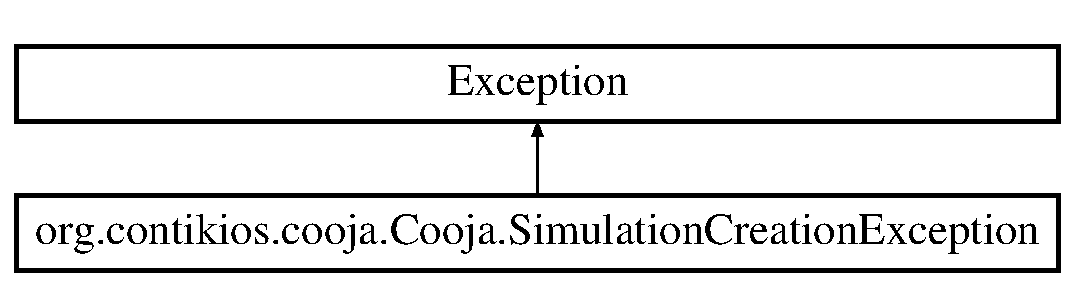
\includegraphics[height=2.000000cm]{classorg_1_1contikios_1_1cooja_1_1Cooja_1_1SimulationCreationException}
\end{center}
\end{figure}
\subsection*{Public Member Functions}
\begin{DoxyCompactItemize}
\item 
\hypertarget{classorg_1_1contikios_1_1cooja_1_1Cooja_1_1SimulationCreationException_ae22e2d685fd114e651eb2d3e678f69fd}{{\bfseries Simulation\-Creation\-Exception} (String message)}\label{classorg_1_1contikios_1_1cooja_1_1Cooja_1_1SimulationCreationException_ae22e2d685fd114e651eb2d3e678f69fd}

\end{DoxyCompactItemize}


The documentation for this class was generated from the following file\-:\begin{DoxyCompactItemize}
\item 
Cooja.\-java\end{DoxyCompactItemize}

\hypertarget{interfaceorg_1_1contikios_1_1cooja_1_1SupportedArguments}{\section{org.\-contikios.\-cooja.\-Supported\-Arguments Interface Reference}
\label{interfaceorg_1_1contikios_1_1cooja_1_1SupportedArguments}\index{org.\-contikios.\-cooja.\-Supported\-Arguments@{org.\-contikios.\-cooja.\-Supported\-Arguments}}
}
\subsection*{Public Member Functions}
\begin{DoxyCompactItemize}
\item 
Class$<$?extends \hyperlink{interfaceorg_1_1contikios_1_1cooja_1_1Mote}{Mote} $>$\mbox{[}$\,$\mbox{]} \hyperlink{interfaceorg_1_1contikios_1_1cooja_1_1SupportedArguments_a59f2db1fa7c770594a08404cf503c155}{motes} () default
\item 
Class$<$?extends \hyperlink{classorg_1_1contikios_1_1cooja_1_1RadioMedium}{Radio\-Medium} $>$\mbox{[}$\,$\mbox{]} \hyperlink{interfaceorg_1_1contikios_1_1cooja_1_1SupportedArguments_a68a7483b2974e2c527ebf82593789764}{radio\-Mediums} () default
\item 
Class$<$?extends \hyperlink{classorg_1_1contikios_1_1cooja_1_1MoteInterface}{Mote\-Interface} $>$\mbox{[}$\,$\mbox{]} \hyperlink{interfaceorg_1_1contikios_1_1cooja_1_1SupportedArguments_a59c91543d5d98c7f21ff8a781e146743}{mote\-Interfaces} () default
\end{DoxyCompactItemize}


\subsection{Detailed Description}
With this annotation, \hyperlink{classorg_1_1contikios_1_1cooja_1_1Cooja}{Cooja} components (e.\-g. mote plugins) can be activated or deactivated depending on the given argument (e.\-g. mote). This may for example be used by a mote plugin that only accepts emulated motes, and that consequently should be hidden in other non-\/emulated motes' plugin menues.

See below code usage examples.

\begin{DoxySeeAlso}{See Also}
\hyperlink{classorg_1_1contikios_1_1cooja_1_1Cooja_a05c932e736bae89b68e5fc74fd6c6648}{Cooja\-::create\-Mote\-Plugins\-Submenu(\-Mote)} 

Visualizer\-::populate\-Skin\-Menu(\-Menu\-Element) 

D\-G\-R\-M\-Visualizer\-Skin
\end{DoxySeeAlso}
\begin{DoxyAuthor}{Author}
Fredrik Osterlind 
\end{DoxyAuthor}


\subsection{Member Function Documentation}
\hypertarget{interfaceorg_1_1contikios_1_1cooja_1_1SupportedArguments_a59c91543d5d98c7f21ff8a781e146743}{\index{org\-::contikios\-::cooja\-::\-Supported\-Arguments@{org\-::contikios\-::cooja\-::\-Supported\-Arguments}!mote\-Interfaces@{mote\-Interfaces}}
\index{mote\-Interfaces@{mote\-Interfaces}!org::contikios::cooja::SupportedArguments@{org\-::contikios\-::cooja\-::\-Supported\-Arguments}}
\subsubsection[{mote\-Interfaces}]{\setlength{\rightskip}{0pt plus 5cm}Class$<$? extends {\bf Mote\-Interface}$>$ \mbox{[}$\,$\mbox{]} org.\-contikios.\-cooja.\-Supported\-Arguments.\-mote\-Interfaces (
\begin{DoxyParamCaption}
{}
\end{DoxyParamCaption}
)\hspace{0.3cm}{\ttfamily [inline]}}}\label{interfaceorg_1_1contikios_1_1cooja_1_1SupportedArguments_a59c91543d5d98c7f21ff8a781e146743}
\begin{DoxyReturn}{Returns}
List of required mote interfaces. 
\end{DoxyReturn}
\hypertarget{interfaceorg_1_1contikios_1_1cooja_1_1SupportedArguments_a59f2db1fa7c770594a08404cf503c155}{\index{org\-::contikios\-::cooja\-::\-Supported\-Arguments@{org\-::contikios\-::cooja\-::\-Supported\-Arguments}!motes@{motes}}
\index{motes@{motes}!org::contikios::cooja::SupportedArguments@{org\-::contikios\-::cooja\-::\-Supported\-Arguments}}
\subsubsection[{motes}]{\setlength{\rightskip}{0pt plus 5cm}Class$<$? extends {\bf Mote}$>$ \mbox{[}$\,$\mbox{]} org.\-contikios.\-cooja.\-Supported\-Arguments.\-motes (
\begin{DoxyParamCaption}
{}
\end{DoxyParamCaption}
)\hspace{0.3cm}{\ttfamily [inline]}}}\label{interfaceorg_1_1contikios_1_1cooja_1_1SupportedArguments_a59f2db1fa7c770594a08404cf503c155}
\begin{DoxyReturn}{Returns}
List of accepted mote classes. 
\end{DoxyReturn}
\hypertarget{interfaceorg_1_1contikios_1_1cooja_1_1SupportedArguments_a68a7483b2974e2c527ebf82593789764}{\index{org\-::contikios\-::cooja\-::\-Supported\-Arguments@{org\-::contikios\-::cooja\-::\-Supported\-Arguments}!radio\-Mediums@{radio\-Mediums}}
\index{radio\-Mediums@{radio\-Mediums}!org::contikios::cooja::SupportedArguments@{org\-::contikios\-::cooja\-::\-Supported\-Arguments}}
\subsubsection[{radio\-Mediums}]{\setlength{\rightskip}{0pt plus 5cm}Class$<$? extends {\bf Radio\-Medium}$>$ \mbox{[}$\,$\mbox{]} org.\-contikios.\-cooja.\-Supported\-Arguments.\-radio\-Mediums (
\begin{DoxyParamCaption}
{}
\end{DoxyParamCaption}
)\hspace{0.3cm}{\ttfamily [inline]}}}\label{interfaceorg_1_1contikios_1_1cooja_1_1SupportedArguments_a68a7483b2974e2c527ebf82593789764}
\begin{DoxyReturn}{Returns}
List of accepted radio medium classes. 
\end{DoxyReturn}


The documentation for this interface was generated from the following file\-:\begin{DoxyCompactItemize}
\item 
Supported\-Arguments.\-java\end{DoxyCompactItemize}

\hypertarget{classorg_1_1contikios_1_1cooja_1_1TimeEvent}{\section{org.\-contikios.\-cooja.\-Time\-Event Class Reference}
\label{classorg_1_1contikios_1_1cooja_1_1TimeEvent}\index{org.\-contikios.\-cooja.\-Time\-Event@{org.\-contikios.\-cooja.\-Time\-Event}}
}
Inheritance diagram for org.\-contikios.\-cooja.\-Time\-Event\-:\begin{figure}[H]
\begin{center}
\leavevmode
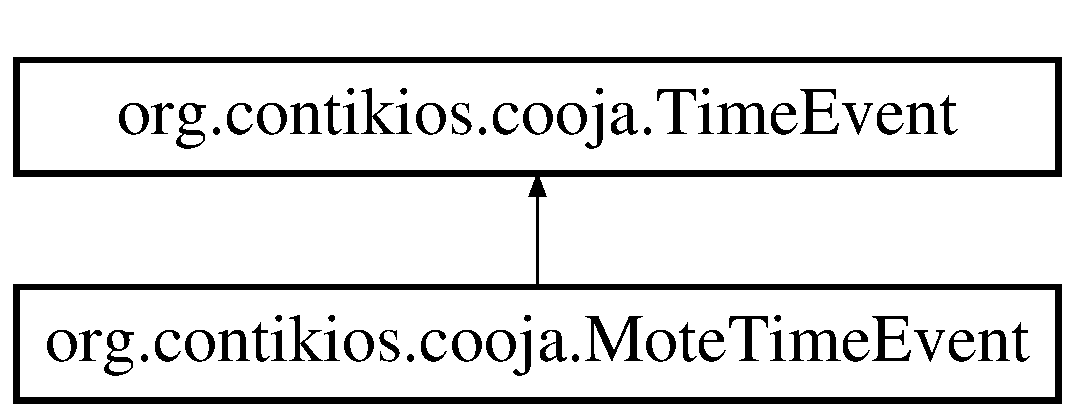
\includegraphics[height=2.000000cm]{classorg_1_1contikios_1_1cooja_1_1TimeEvent}
\end{center}
\end{figure}
\subsection*{Public Member Functions}
\begin{DoxyCompactItemize}
\item 
\hypertarget{classorg_1_1contikios_1_1cooja_1_1TimeEvent_ac94a97a97a1b979c1e0fd5488cf55ce8}{{\bfseries Time\-Event} (long time)}\label{classorg_1_1contikios_1_1cooja_1_1TimeEvent_ac94a97a97a1b979c1e0fd5488cf55ce8}

\item 
\hypertarget{classorg_1_1contikios_1_1cooja_1_1TimeEvent_a05a69143bc9566dd6cc516c4d0ad523b}{{\bfseries Time\-Event} (long time, String name)}\label{classorg_1_1contikios_1_1cooja_1_1TimeEvent_a05a69143bc9566dd6cc516c4d0ad523b}

\item 
\hypertarget{classorg_1_1contikios_1_1cooja_1_1TimeEvent_af4ea02d75ed7b85008d4a900eadd372b}{final long {\bfseries get\-Time} ()}\label{classorg_1_1contikios_1_1cooja_1_1TimeEvent_af4ea02d75ed7b85008d4a900eadd372b}

\item 
\hypertarget{classorg_1_1contikios_1_1cooja_1_1TimeEvent_a65fdda82f90f09e2bca14ff651c70d2f}{boolean {\bfseries is\-Scheduled} ()}\label{classorg_1_1contikios_1_1cooja_1_1TimeEvent_a65fdda82f90f09e2bca14ff651c70d2f}

\item 
\hypertarget{classorg_1_1contikios_1_1cooja_1_1TimeEvent_a4b66d6464ac9502afe9faefa7c83f1b1}{boolean {\bfseries remove} ()}\label{classorg_1_1contikios_1_1cooja_1_1TimeEvent_a4b66d6464ac9502afe9faefa7c83f1b1}

\item 
\hypertarget{classorg_1_1contikios_1_1cooja_1_1TimeEvent_a8818e9e93d5ae15c77a207535f47ebce}{abstract void {\bfseries execute} (long t)}\label{classorg_1_1contikios_1_1cooja_1_1TimeEvent_a8818e9e93d5ae15c77a207535f47ebce}

\item 
\hypertarget{classorg_1_1contikios_1_1cooja_1_1TimeEvent_af01fa994a7eef07dc1da46aa41bc4dc0}{String {\bfseries get\-Short} ()}\label{classorg_1_1contikios_1_1cooja_1_1TimeEvent_af01fa994a7eef07dc1da46aa41bc4dc0}

\end{DoxyCompactItemize}
\subsection*{Protected Attributes}
\begin{DoxyCompactItemize}
\item 
\hypertarget{classorg_1_1contikios_1_1cooja_1_1TimeEvent_a932d203ebb83d90339e2884d07c1824f}{long {\bfseries time}}\label{classorg_1_1contikios_1_1cooja_1_1TimeEvent_a932d203ebb83d90339e2884d07c1824f}

\end{DoxyCompactItemize}


\subsection{Detailed Description}
\begin{DoxyAuthor}{Author}
Joakim Eriksson (ported to C\-O\-O\-J\-A by Fredrik Osterlind) 
\end{DoxyAuthor}


The documentation for this class was generated from the following file\-:\begin{DoxyCompactItemize}
\item 
Time\-Event.\-java\end{DoxyCompactItemize}

\hypertarget{classorg_1_1contikios_1_1cooja_1_1VisPlugin}{\section{org.\-contikios.\-cooja.\-Vis\-Plugin Class Reference}
\label{classorg_1_1contikios_1_1cooja_1_1VisPlugin}\index{org.\-contikios.\-cooja.\-Vis\-Plugin@{org.\-contikios.\-cooja.\-Vis\-Plugin}}
}
Inheritance diagram for org.\-contikios.\-cooja.\-Vis\-Plugin\-:\begin{figure}[H]
\begin{center}
\leavevmode
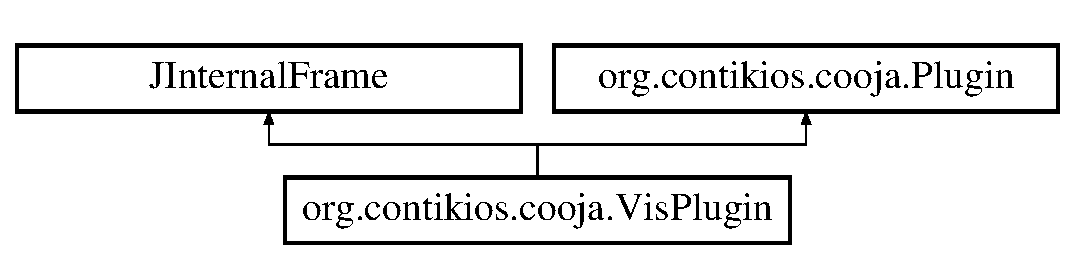
\includegraphics[height=2.000000cm]{classorg_1_1contikios_1_1cooja_1_1VisPlugin}
\end{center}
\end{figure}
\subsection*{Classes}
\begin{DoxyCompactItemize}
\item 
class {\bfseries Plugin\-Requires\-Visualization\-Exception}
\end{DoxyCompactItemize}
\subsection*{Public Member Functions}
\begin{DoxyCompactItemize}
\item 
\hypertarget{classorg_1_1contikios_1_1cooja_1_1VisPlugin_a141a4f9ecee96ae38118d2285674c320}{{\bfseries Vis\-Plugin} (String title, final \hyperlink{classorg_1_1contikios_1_1cooja_1_1Cooja}{Cooja} gui)}\label{classorg_1_1contikios_1_1cooja_1_1VisPlugin_a141a4f9ecee96ae38118d2285674c320}

\item 
\hypertarget{classorg_1_1contikios_1_1cooja_1_1VisPlugin_aea37414f11100bcb1d265d71887b812b}{{\bfseries Vis\-Plugin} (String title, final \hyperlink{classorg_1_1contikios_1_1cooja_1_1Cooja}{Cooja} gui, boolean requires\-Vis)}\label{classorg_1_1contikios_1_1cooja_1_1VisPlugin_aea37414f11100bcb1d265d71887b812b}

\item 
J\-Internal\-Frame \hyperlink{classorg_1_1contikios_1_1cooja_1_1VisPlugin_a4c73dd97f27405a0804a2473d3e75e35}{get\-Cooja} ()
\item 
Collection$<$ Element $>$ \hyperlink{classorg_1_1contikios_1_1cooja_1_1VisPlugin_a2c15dd2d95364a708dde19b7b54fa974}{get\-Config\-X\-M\-L} ()
\item 
boolean \hyperlink{classorg_1_1contikios_1_1cooja_1_1VisPlugin_ad709d713ee9528c843400984ae183c6f}{set\-Config\-X\-M\-L} (Collection$<$ Element $>$ config\-X\-M\-L, boolean vis\-Available)
\item 
void \hyperlink{classorg_1_1contikios_1_1cooja_1_1VisPlugin_a34e1bee73bd2b86e39bb267f450e624f}{start\-Plugin} ()
\item 
void \hyperlink{classorg_1_1contikios_1_1cooja_1_1VisPlugin_ab010d744bcc4f590f7edd2e32e5f758d}{close\-Plugin} ()
\end{DoxyCompactItemize}


\subsection{Detailed Description}
Visualized plugins can extend \hyperlink{classorg_1_1contikios_1_1cooja_1_1VisPlugin}{Vis\-Plugin} for basic visualization functionality. \hyperlink{classorg_1_1contikios_1_1cooja_1_1VisPlugin}{Vis\-Plugin} extends J\-Internal\-Frame, the graphical component used by plugins. \hyperlink{classorg_1_1contikios_1_1cooja_1_1VisPlugin}{Vis\-Plugin} implementations may hence directly add buttons to themselves.

Note that plugins of this type can only be started if C\-O\-O\-J\-A is visualized. Hence, these plugins will not be started during nightly Contiki tests.

\begin{DoxySeeAlso}{See Also}
Sim\-Control 

Plugin\-Requires\-Visualization\-Exception 
\end{DoxySeeAlso}
\begin{DoxyAuthor}{Author}
Fredrik Osterlind 
\end{DoxyAuthor}


\subsection{Member Function Documentation}
\hypertarget{classorg_1_1contikios_1_1cooja_1_1VisPlugin_ab010d744bcc4f590f7edd2e32e5f758d}{\index{org\-::contikios\-::cooja\-::\-Vis\-Plugin@{org\-::contikios\-::cooja\-::\-Vis\-Plugin}!close\-Plugin@{close\-Plugin}}
\index{close\-Plugin@{close\-Plugin}!org::contikios::cooja::VisPlugin@{org\-::contikios\-::cooja\-::\-Vis\-Plugin}}
\subsubsection[{close\-Plugin}]{\setlength{\rightskip}{0pt plus 5cm}void org.\-contikios.\-cooja.\-Vis\-Plugin.\-close\-Plugin (
\begin{DoxyParamCaption}
{}
\end{DoxyParamCaption}
)\hspace{0.3cm}{\ttfamily [inline]}}}\label{classorg_1_1contikios_1_1cooja_1_1VisPlugin_ab010d744bcc4f590f7edd2e32e5f758d}
This method is called when an opened plugin is about to close. It should release any resources such as registered observers or opened interface visualizers. 

Implements \hyperlink{interfaceorg_1_1contikios_1_1cooja_1_1Plugin_a87f92ae1a613ed6f3665a953ab748430}{org.\-contikios.\-cooja.\-Plugin}.

\hypertarget{classorg_1_1contikios_1_1cooja_1_1VisPlugin_a2c15dd2d95364a708dde19b7b54fa974}{\index{org\-::contikios\-::cooja\-::\-Vis\-Plugin@{org\-::contikios\-::cooja\-::\-Vis\-Plugin}!get\-Config\-X\-M\-L@{get\-Config\-X\-M\-L}}
\index{get\-Config\-X\-M\-L@{get\-Config\-X\-M\-L}!org::contikios::cooja::VisPlugin@{org\-::contikios\-::cooja\-::\-Vis\-Plugin}}
\subsubsection[{get\-Config\-X\-M\-L}]{\setlength{\rightskip}{0pt plus 5cm}Collection$<$Element$>$ org.\-contikios.\-cooja.\-Vis\-Plugin.\-get\-Config\-X\-M\-L (
\begin{DoxyParamCaption}
{}
\end{DoxyParamCaption}
)\hspace{0.3cm}{\ttfamily [inline]}}}\label{classorg_1_1contikios_1_1cooja_1_1VisPlugin_a2c15dd2d95364a708dde19b7b54fa974}
Returns X\-M\-L elements representing the current config of this plugin. This is fetched by the simulator for example when saving a simulation configuration file. For example a plugin may return the current size and position. This method should however not return state specific information such as the value of a mote L\-E\-D, or total number of motes. (All nodes are restarted when loading a simulation.)

\begin{DoxySeeAlso}{See Also}
\#set\-Config\-X\-M\-L(\-Collection, boolean) 
\end{DoxySeeAlso}
\begin{DoxyReturn}{Returns}
X\-M\-L elements representing the current radio medium config 
\end{DoxyReturn}


Implements \hyperlink{interfaceorg_1_1contikios_1_1cooja_1_1Plugin_acf14af975741b1de50749b358cd671a7}{org.\-contikios.\-cooja.\-Plugin}.

\hypertarget{classorg_1_1contikios_1_1cooja_1_1VisPlugin_a4c73dd97f27405a0804a2473d3e75e35}{\index{org\-::contikios\-::cooja\-::\-Vis\-Plugin@{org\-::contikios\-::cooja\-::\-Vis\-Plugin}!get\-Cooja@{get\-Cooja}}
\index{get\-Cooja@{get\-Cooja}!org::contikios::cooja::VisPlugin@{org\-::contikios\-::cooja\-::\-Vis\-Plugin}}
\subsubsection[{get\-Cooja}]{\setlength{\rightskip}{0pt plus 5cm}J\-Internal\-Frame org.\-contikios.\-cooja.\-Vis\-Plugin.\-get\-Cooja (
\begin{DoxyParamCaption}
{}
\end{DoxyParamCaption}
)\hspace{0.3cm}{\ttfamily [inline]}}}\label{classorg_1_1contikios_1_1cooja_1_1VisPlugin_a4c73dd97f27405a0804a2473d3e75e35}
Graphical component of plugin (if any) 

Implements \hyperlink{interfaceorg_1_1contikios_1_1cooja_1_1Plugin_ae19ca3da5d492cfc80836f304f71b32a}{org.\-contikios.\-cooja.\-Plugin}.

\hypertarget{classorg_1_1contikios_1_1cooja_1_1VisPlugin_ad709d713ee9528c843400984ae183c6f}{\index{org\-::contikios\-::cooja\-::\-Vis\-Plugin@{org\-::contikios\-::cooja\-::\-Vis\-Plugin}!set\-Config\-X\-M\-L@{set\-Config\-X\-M\-L}}
\index{set\-Config\-X\-M\-L@{set\-Config\-X\-M\-L}!org::contikios::cooja::VisPlugin@{org\-::contikios\-::cooja\-::\-Vis\-Plugin}}
\subsubsection[{set\-Config\-X\-M\-L}]{\setlength{\rightskip}{0pt plus 5cm}boolean org.\-contikios.\-cooja.\-Vis\-Plugin.\-set\-Config\-X\-M\-L (
\begin{DoxyParamCaption}
\item[{Collection$<$ Element $>$}]{config\-X\-M\-L, }
\item[{boolean}]{vis\-Available}
\end{DoxyParamCaption}
)\hspace{0.3cm}{\ttfamily [inline]}}}\label{classorg_1_1contikios_1_1cooja_1_1VisPlugin_ad709d713ee9528c843400984ae183c6f}
Sets the current plugin config depending on the given X\-M\-L elements.

\begin{DoxySeeAlso}{See Also}
\hyperlink{classorg_1_1contikios_1_1cooja_1_1VisPlugin_a2c15dd2d95364a708dde19b7b54fa974}{get\-Config\-X\-M\-L()} 
\end{DoxySeeAlso}

\begin{DoxyParams}{Parameters}
{\em config\-X\-M\-L} & Config X\-M\-L elements \\
\hline
\end{DoxyParams}
\begin{DoxyReturn}{Returns}
True if config was set successfully, false otherwise 
\end{DoxyReturn}


Implements \hyperlink{interfaceorg_1_1contikios_1_1cooja_1_1Plugin_a1a7b2031b097da13170429ce7f9dc39e}{org.\-contikios.\-cooja.\-Plugin}.

\hypertarget{classorg_1_1contikios_1_1cooja_1_1VisPlugin_a34e1bee73bd2b86e39bb267f450e624f}{\index{org\-::contikios\-::cooja\-::\-Vis\-Plugin@{org\-::contikios\-::cooja\-::\-Vis\-Plugin}!start\-Plugin@{start\-Plugin}}
\index{start\-Plugin@{start\-Plugin}!org::contikios::cooja::VisPlugin@{org\-::contikios\-::cooja\-::\-Vis\-Plugin}}
\subsubsection[{start\-Plugin}]{\setlength{\rightskip}{0pt plus 5cm}void org.\-contikios.\-cooja.\-Vis\-Plugin.\-start\-Plugin (
\begin{DoxyParamCaption}
{}
\end{DoxyParamCaption}
)\hspace{0.3cm}{\ttfamily [inline]}}}\label{classorg_1_1contikios_1_1cooja_1_1VisPlugin_a34e1bee73bd2b86e39bb267f450e624f}
This method is called to activate a new plugin, after constructing it. If a simulation is loaded, this method is called after \hyperlink{}{set\-Config\-X\-M\-L(\-Collection, boolean)}.

\begin{DoxySeeAlso}{See Also}
\#set\-Config\-X\-M\-L(\-Collection, boolean) 

\hyperlink{classorg_1_1contikios_1_1cooja_1_1VisPlugin_ab010d744bcc4f590f7edd2e32e5f758d}{close\-Plugin()} 
\end{DoxySeeAlso}


Implements \hyperlink{interfaceorg_1_1contikios_1_1cooja_1_1Plugin_aae8a585e3a659cc585859a5728a42d15}{org.\-contikios.\-cooja.\-Plugin}.



The documentation for this class was generated from the following file\-:\begin{DoxyCompactItemize}
\item 
Vis\-Plugin.\-java\end{DoxyCompactItemize}

\hypertarget{interfaceorg_1_1contikios_1_1cooja_1_1Watchpoint}{\section{org.\-contikios.\-cooja.\-Watchpoint Interface Reference}
\label{interfaceorg_1_1contikios_1_1cooja_1_1Watchpoint}\index{org.\-contikios.\-cooja.\-Watchpoint@{org.\-contikios.\-cooja.\-Watchpoint}}
}
\subsection*{Public Member Functions}
\begin{DoxyCompactItemize}
\item 
\hypertarget{interfaceorg_1_1contikios_1_1cooja_1_1Watchpoint_a3c68dab7c90c85695e85bab407067e7f}{\hyperlink{interfaceorg_1_1contikios_1_1cooja_1_1WatchpointMote}{Watchpoint\-Mote} {\bfseries get\-Mote} ()}\label{interfaceorg_1_1contikios_1_1cooja_1_1Watchpoint_a3c68dab7c90c85695e85bab407067e7f}

\item 
\hypertarget{interfaceorg_1_1contikios_1_1cooja_1_1Watchpoint_a2ee61d65c4dc1ea45f3982a5b858c27e}{Color {\bfseries get\-Color} ()}\label{interfaceorg_1_1contikios_1_1cooja_1_1Watchpoint_a2ee61d65c4dc1ea45f3982a5b858c27e}

\item 
\hypertarget{interfaceorg_1_1contikios_1_1cooja_1_1Watchpoint_addff38d640bdc980d2f15067180a6719}{void {\bfseries set\-Color} (Color new\-Color)}\label{interfaceorg_1_1contikios_1_1cooja_1_1Watchpoint_addff38d640bdc980d2f15067180a6719}

\item 
\hypertarget{interfaceorg_1_1contikios_1_1cooja_1_1Watchpoint_a1c5ec940d4fd286228b342b900489c2f}{String {\bfseries get\-Description} ()}\label{interfaceorg_1_1contikios_1_1cooja_1_1Watchpoint_a1c5ec940d4fd286228b342b900489c2f}

\item 
\hypertarget{interfaceorg_1_1contikios_1_1cooja_1_1Watchpoint_ae0df94ae24cd0c0fe3596ad8dde51750}{void {\bfseries set\-User\-Message} (String msg)}\label{interfaceorg_1_1contikios_1_1cooja_1_1Watchpoint_ae0df94ae24cd0c0fe3596ad8dde51750}

\item 
\hypertarget{interfaceorg_1_1contikios_1_1cooja_1_1Watchpoint_a412c90524ecb0a39f040dc59724bddb8}{String {\bfseries get\-User\-Message} ()}\label{interfaceorg_1_1contikios_1_1cooja_1_1Watchpoint_a412c90524ecb0a39f040dc59724bddb8}

\item 
\hypertarget{interfaceorg_1_1contikios_1_1cooja_1_1Watchpoint_ab6ccaff743ab6775e51d88c9a06fb120}{File {\bfseries get\-Code\-File} ()}\label{interfaceorg_1_1contikios_1_1cooja_1_1Watchpoint_ab6ccaff743ab6775e51d88c9a06fb120}

\item 
\hypertarget{interfaceorg_1_1contikios_1_1cooja_1_1Watchpoint_ab646e1a6f6783b1e7ed284a611caa4a7}{int {\bfseries get\-Line\-Number} ()}\label{interfaceorg_1_1contikios_1_1cooja_1_1Watchpoint_ab646e1a6f6783b1e7ed284a611caa4a7}

\item 
\hypertarget{interfaceorg_1_1contikios_1_1cooja_1_1Watchpoint_a7f721680839841d479e2783fbe8c6268}{int {\bfseries get\-Executable\-Address} ()}\label{interfaceorg_1_1contikios_1_1cooja_1_1Watchpoint_a7f721680839841d479e2783fbe8c6268}

\item 
\hypertarget{interfaceorg_1_1contikios_1_1cooja_1_1Watchpoint_a0526ee450f11d884f4d21e6ea5f6d560}{void {\bfseries set\-Stops\-Simulation} (boolean b)}\label{interfaceorg_1_1contikios_1_1cooja_1_1Watchpoint_a0526ee450f11d884f4d21e6ea5f6d560}

\item 
\hypertarget{interfaceorg_1_1contikios_1_1cooja_1_1Watchpoint_ac0579bce86f45786c149702f7e1a423d}{boolean {\bfseries stops\-Simulation} ()}\label{interfaceorg_1_1contikios_1_1cooja_1_1Watchpoint_ac0579bce86f45786c149702f7e1a423d}

\end{DoxyCompactItemize}


\subsection{Detailed Description}
\begin{DoxyAuthor}{Author}
Fredrik Osterlind 
\end{DoxyAuthor}


The documentation for this interface was generated from the following file\-:\begin{DoxyCompactItemize}
\item 
Watchpoint.\-java\end{DoxyCompactItemize}

\hypertarget{interfaceorg_1_1contikios_1_1cooja_1_1WatchpointMote_1_1WatchpointListener}{\section{org.\-contikios.\-cooja.\-Watchpoint\-Mote.\-Watchpoint\-Listener Interface Reference}
\label{interfaceorg_1_1contikios_1_1cooja_1_1WatchpointMote_1_1WatchpointListener}\index{org.\-contikios.\-cooja.\-Watchpoint\-Mote.\-Watchpoint\-Listener@{org.\-contikios.\-cooja.\-Watchpoint\-Mote.\-Watchpoint\-Listener}}
}
\subsection*{Public Member Functions}
\begin{DoxyCompactItemize}
\item 
\hypertarget{interfaceorg_1_1contikios_1_1cooja_1_1WatchpointMote_1_1WatchpointListener_a20219204decf909d4993102671ad8b8e}{void {\bfseries watchpoint\-Triggered} (\hyperlink{interfaceorg_1_1contikios_1_1cooja_1_1Watchpoint}{Watchpoint} watchpoint)}\label{interfaceorg_1_1contikios_1_1cooja_1_1WatchpointMote_1_1WatchpointListener_a20219204decf909d4993102671ad8b8e}

\item 
\hypertarget{interfaceorg_1_1contikios_1_1cooja_1_1WatchpointMote_1_1WatchpointListener_ac6617c56488266f2d6709bbcdcda9583}{void {\bfseries watchpoints\-Changed} ()}\label{interfaceorg_1_1contikios_1_1cooja_1_1WatchpointMote_1_1WatchpointListener_ac6617c56488266f2d6709bbcdcda9583}

\end{DoxyCompactItemize}


The documentation for this interface was generated from the following file\-:\begin{DoxyCompactItemize}
\item 
Watchpoint\-Mote.\-java\end{DoxyCompactItemize}

\hypertarget{interfaceorg_1_1contikios_1_1cooja_1_1WatchpointMote}{\section{org.\-contikios.\-cooja.\-Watchpoint\-Mote Interface Reference}
\label{interfaceorg_1_1contikios_1_1cooja_1_1WatchpointMote}\index{org.\-contikios.\-cooja.\-Watchpoint\-Mote@{org.\-contikios.\-cooja.\-Watchpoint\-Mote}}
}
Inheritance diagram for org.\-contikios.\-cooja.\-Watchpoint\-Mote\-:\begin{figure}[H]
\begin{center}
\leavevmode
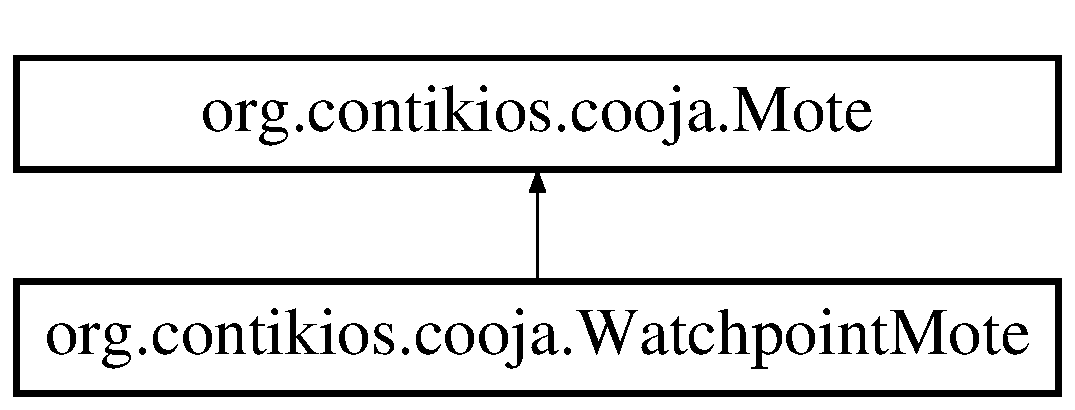
\includegraphics[height=2.000000cm]{interfaceorg_1_1contikios_1_1cooja_1_1WatchpointMote}
\end{center}
\end{figure}
\subsection*{Classes}
\begin{DoxyCompactItemize}
\item 
interface \hyperlink{interfaceorg_1_1contikios_1_1cooja_1_1WatchpointMote_1_1WatchpointListener}{Watchpoint\-Listener}
\end{DoxyCompactItemize}
\subsection*{Public Member Functions}
\begin{DoxyCompactItemize}
\item 
void \hyperlink{interfaceorg_1_1contikios_1_1cooja_1_1WatchpointMote_a422ed917d13f2e76099cec13cea7be4c}{add\-Watchpoint\-Listener} (\hyperlink{interfaceorg_1_1contikios_1_1cooja_1_1WatchpointMote_1_1WatchpointListener}{Watchpoint\-Listener} listener)
\item 
void \hyperlink{interfaceorg_1_1contikios_1_1cooja_1_1WatchpointMote_a57ad0caf798fd458fef468f40977b9f0}{remove\-Watchpoint\-Listener} (\hyperlink{interfaceorg_1_1contikios_1_1cooja_1_1WatchpointMote_1_1WatchpointListener}{Watchpoint\-Listener} listener)
\item 
\hyperlink{interfaceorg_1_1contikios_1_1cooja_1_1WatchpointMote_1_1WatchpointListener}{Watchpoint\-Listener}\mbox{[}$\,$\mbox{]} \hyperlink{interfaceorg_1_1contikios_1_1cooja_1_1WatchpointMote_abce6d5e098f44df1a6991cdd3f0b4afa}{get\-Watchpoint\-Listeners} ()
\item 
\hypertarget{interfaceorg_1_1contikios_1_1cooja_1_1WatchpointMote_add650fce714a1f156c06defc0a1d9057}{\hyperlink{interfaceorg_1_1contikios_1_1cooja_1_1Watchpoint}{Watchpoint} {\bfseries add\-Breakpoint} (File code\-File, int line\-Nr, int address)}\label{interfaceorg_1_1contikios_1_1cooja_1_1WatchpointMote_add650fce714a1f156c06defc0a1d9057}

\item 
\hypertarget{interfaceorg_1_1contikios_1_1cooja_1_1WatchpointMote_a0621db6f7fd4b2afa17e8e550973564d}{void {\bfseries remove\-Breakpoint} (\hyperlink{interfaceorg_1_1contikios_1_1cooja_1_1Watchpoint}{Watchpoint} watchpoint)}\label{interfaceorg_1_1contikios_1_1cooja_1_1WatchpointMote_a0621db6f7fd4b2afa17e8e550973564d}

\item 
\hypertarget{interfaceorg_1_1contikios_1_1cooja_1_1WatchpointMote_aef2586e726f86f2cd99ae6789cc2c516}{\hyperlink{interfaceorg_1_1contikios_1_1cooja_1_1Watchpoint}{Watchpoint}\mbox{[}$\,$\mbox{]} {\bfseries get\-Breakpoints} ()}\label{interfaceorg_1_1contikios_1_1cooja_1_1WatchpointMote_aef2586e726f86f2cd99ae6789cc2c516}

\item 
\hypertarget{interfaceorg_1_1contikios_1_1cooja_1_1WatchpointMote_ac70a8cf1a7b58e3adb5d9d4586ad6e65}{boolean {\bfseries breakpoint\-Exists} (int address)}\label{interfaceorg_1_1contikios_1_1cooja_1_1WatchpointMote_ac70a8cf1a7b58e3adb5d9d4586ad6e65}

\item 
\hypertarget{interfaceorg_1_1contikios_1_1cooja_1_1WatchpointMote_a9691683f558f6b84e05a5ae530d7d952}{boolean {\bfseries breakpoint\-Exists} (File file, int line\-Nr)}\label{interfaceorg_1_1contikios_1_1cooja_1_1WatchpointMote_a9691683f558f6b84e05a5ae530d7d952}

\item 
\hypertarget{interfaceorg_1_1contikios_1_1cooja_1_1WatchpointMote_aec062cf53c898441755c9257913c154e}{int {\bfseries get\-Executable\-Address\-Of} (File file, int line\-Nr)}\label{interfaceorg_1_1contikios_1_1cooja_1_1WatchpointMote_aec062cf53c898441755c9257913c154e}

\end{DoxyCompactItemize}


\subsection{Detailed Description}
\begin{DoxyAuthor}{Author}
Fredrik Osterlind 
\end{DoxyAuthor}


\subsection{Member Function Documentation}
\hypertarget{interfaceorg_1_1contikios_1_1cooja_1_1WatchpointMote_a422ed917d13f2e76099cec13cea7be4c}{\index{org\-::contikios\-::cooja\-::\-Watchpoint\-Mote@{org\-::contikios\-::cooja\-::\-Watchpoint\-Mote}!add\-Watchpoint\-Listener@{add\-Watchpoint\-Listener}}
\index{add\-Watchpoint\-Listener@{add\-Watchpoint\-Listener}!org::contikios::cooja::WatchpointMote@{org\-::contikios\-::cooja\-::\-Watchpoint\-Mote}}
\subsubsection[{add\-Watchpoint\-Listener}]{\setlength{\rightskip}{0pt plus 5cm}void org.\-contikios.\-cooja.\-Watchpoint\-Mote.\-add\-Watchpoint\-Listener (
\begin{DoxyParamCaption}
\item[{{\bf Watchpoint\-Listener}}]{listener}
\end{DoxyParamCaption}
)}}\label{interfaceorg_1_1contikios_1_1cooja_1_1WatchpointMote_a422ed917d13f2e76099cec13cea7be4c}
Adds a breakpoint listener. The listener will be notified when breakpoints are added, removed or triggered.


\begin{DoxyParams}{Parameters}
{\em listener} & Action listener \\
\hline
\end{DoxyParams}
\hypertarget{interfaceorg_1_1contikios_1_1cooja_1_1WatchpointMote_abce6d5e098f44df1a6991cdd3f0b4afa}{\index{org\-::contikios\-::cooja\-::\-Watchpoint\-Mote@{org\-::contikios\-::cooja\-::\-Watchpoint\-Mote}!get\-Watchpoint\-Listeners@{get\-Watchpoint\-Listeners}}
\index{get\-Watchpoint\-Listeners@{get\-Watchpoint\-Listeners}!org::contikios::cooja::WatchpointMote@{org\-::contikios\-::cooja\-::\-Watchpoint\-Mote}}
\subsubsection[{get\-Watchpoint\-Listeners}]{\setlength{\rightskip}{0pt plus 5cm}{\bf Watchpoint\-Listener} \mbox{[}$\,$\mbox{]} org.\-contikios.\-cooja.\-Watchpoint\-Mote.\-get\-Watchpoint\-Listeners (
\begin{DoxyParamCaption}
{}
\end{DoxyParamCaption}
)}}\label{interfaceorg_1_1contikios_1_1cooja_1_1WatchpointMote_abce6d5e098f44df1a6991cdd3f0b4afa}
\begin{DoxyReturn}{Returns}
All registered listeners 
\end{DoxyReturn}
\hypertarget{interfaceorg_1_1contikios_1_1cooja_1_1WatchpointMote_a57ad0caf798fd458fef468f40977b9f0}{\index{org\-::contikios\-::cooja\-::\-Watchpoint\-Mote@{org\-::contikios\-::cooja\-::\-Watchpoint\-Mote}!remove\-Watchpoint\-Listener@{remove\-Watchpoint\-Listener}}
\index{remove\-Watchpoint\-Listener@{remove\-Watchpoint\-Listener}!org::contikios::cooja::WatchpointMote@{org\-::contikios\-::cooja\-::\-Watchpoint\-Mote}}
\subsubsection[{remove\-Watchpoint\-Listener}]{\setlength{\rightskip}{0pt plus 5cm}void org.\-contikios.\-cooja.\-Watchpoint\-Mote.\-remove\-Watchpoint\-Listener (
\begin{DoxyParamCaption}
\item[{{\bf Watchpoint\-Listener}}]{listener}
\end{DoxyParamCaption}
)}}\label{interfaceorg_1_1contikios_1_1cooja_1_1WatchpointMote_a57ad0caf798fd458fef468f40977b9f0}
Removes previously registered listener.


\begin{DoxyParams}{Parameters}
{\em listener} & Listeners \\
\hline
\end{DoxyParams}


The documentation for this interface was generated from the following file\-:\begin{DoxyCompactItemize}
\item 
Watchpoint\-Mote.\-java\end{DoxyCompactItemize}

%--- End generated contents ---

% Index
\newpage
\phantomsection
\addcontentsline{toc}{chapter}{Index}
\printindex

\end{document}
